% \documentclass[a4paper,10pt]{article}
\documentclass[a5paper,10pt]{article}
\usepackage[utf8x]{inputenc}

% \usepackage[a4paper,landscape]{geometry}
\usepackage[a4paper]{geometry}
\usepackage{multicol}
\usepackage{graphicx}
\usepackage{url}

% \newcommand{\picinclude}[1]{\includegraphics[width=0.5\textwidth,height=1.0\textheight]{#1}}
\newcommand{\picinclude}[1]{\includegraphics[height=1.0\textheight]{#1}}

%opening
\title{George Fox -- Aufzeichnungen und Briefe des ersten Quäkers}
\author{Übersetzerin: Margrit Stähelin \\ 
Originalerscheinung: Tübingen 1908 \\ 
Verlag I.C.B. Mohr (Paul Siebek) \\
Nachbearbeitung: Olaf Radicke
}

\date{Erstellungsdatum: \today}

\begin{document}

\maketitle

\begin{figure}[h!]
 \centering
 
\includegraphics{./cc-lizenz-by.png}
 % cc-lizenz-by.png: 32x32 pixel, 72dpi, 1.13x1.13 cm, bb=0 0 32 32
\end{figure}

\section{Vorwort}
\label{sec:vorwort}

Diese Dokument basiert auf ein Scann des Werkes ``George Fox -- 
Aufzeichnungen und Briefe des ersten Quäkers''. Troz intensiver Bemühungen war es mir nicht
möglich zu ermitteln ob und wer das Urheberecht an dem Werk besitzt. Sollte jemand zur
klärung beitragen können, bitte ich um Hinweise an mich!

\begin{center}
Olaf Radicke \\
Ludwig-Richter-Str. 28 \\
80687 München \\
briefkasten@olaf-radicke.de \\
\end{center}

Ich glaube das der Text für das Quakertum in Deutschland so unverzichtbar ist,
das ich mich entschlossenhabe trozdem den Text (wieder) zu veröffentlichen. Meine 
Textbearbeitung stelle ich unter einer \textit{Creative Commons-Lizenz lizenziert}: 
Namensnennung-Weitergabe unter gleichen Bedingungen 3.0 Deutschland (CC BY-SA 3.0).

\subsection{Sie dürfen}

\begin{itemize}
 \item das Werk bzw. den Inhalt vervielfältigen, verbreiten und öffentlich zugänglich machen
 \item Abwandlungen und Bearbeitungen des Werkes bzw. Inhaltes anfertigen
 \item das Werk kommerziell nutzen
\end{itemize}


\subsection{Zu den folgenden Bedingungen}



\begin{description}
 \item[Namensnennung] Sie müssen den Namen des Autors/Rechteinhabers in der von ihm 
festgelegten Weise nennen.


 \item[Weitergabe unter gleichen Bedingungen] Wenn Sie das lizenzierte Werk bzw. den 
lizenzierten Inhalt bearbeiten oder in anderer Weise erkennbar als Grundlage für 
eigenes Schaffen verwenden, dürfen Sie die daraufhin neu entstandenen Werke bzw. 
Inhalte nur unter Verwendung von Lizenzbedingungen weitergeben, die mit denen dieses 
Lizenzvertrages identisch oder vergleichbar sind.
 \end{description}

\subsection{Wobei gilt}

\begin{description}
    \item[Verzichtserklärung] Jede der vorgenannten Bedingungen kann aufgehoben werden, 
	  sofern Sie die ausdrückliche Einwilligung des Rechteinhabers dazu erhalten.
    \item[Public Domain (gemeinfreie oder nicht-schützbare Inhalte)] Soweit das Werk, 
	  der Inhalt oder irgendein Teil davon zur Public Domain der jeweiligen Rechtsordnung 
	  gehört, wird dieser Status von der Lizenz in keiner Weise berührt.
    \item[Sonstige Rechte] Die Lizenz hat keinerlei Einfluss auf die folgenden Rechte:
      \begin{itemize}
          \item Die Rechte, die jedermann wegen der Schranken des Urheberrechts oder 
		aufgrund gesetzlicher Erlaubnisse zustehen (in einigen Ländern als 
		grundsätzliche Doktrin des fair use etabliert);
          \item Das Urheberpersönlichkeitsrecht des Rechteinhabers;
          \item Rechte anderer Personen, entweder am Lizenzgegenstand selber oder bezüglich 
		seiner Verwendung, zum Beispiel Persönlichkeitsrechte abgebildeter Personen.
      \end{itemize}
    \item[Hinweis] Im Falle einer Verbreitung müssen Sie anderen alle Lizenzbedingungen 
	  mitteilen, die für dieses Werk gelten. Am einfachsten ist es, an entsprechender 
	  Stelle einen Link auf diese Seite einzubinden.

 \end{description}

Diese "Commons Deed" ist lediglich eine vereinfachte Zusammenfassung des rechtsverbindlichen 
Lizenzvertrages in allgemeinverständlicher Sprache. Deteils, Erleuterungen und vollständigen
Lizenz-Text erhalten Sie unter \url{http://creativecommons.org/licenses/by-sa/3.0/de/}

 \centering

% \begin{multicols}{2}

% \begin{multicols}{2}
%\begin{figure}[h!]
\picinclude{./vorwort/p_v01.jpg} 
\picinclude{./vorwort/p_v02.jpg} 
\picinclude{./vorwort/p_v03.jpg} 
\picinclude{./vorwort/p_v04.jpg} 
\picinclude{./vorwort/p_v05.jpg} 
\picinclude{./vorwort/p_v06.jpg} 
\picinclude{./vorwort/p_v07.jpg} 
\picinclude{./vorwort/p_v08.jpg} 
\picinclude{./vorwort/p_v09.jpg} 
\picinclude{./vorwort/p_v10.jpg} 
\picinclude{./vorwort/p_v11.jpg} 
\picinclude{./vorwort/p_v12.jpg} 
\picinclude{./vorwort/p_v13.jpg} 
\picinclude{./vorwort/p_v14.jpg} 
\picinclude{./vorwort/p_v15.jpg} 
\picinclude{./vorwort/p_v16.jpg} 
\picinclude{./vorwort/p_v17.jpg} 
\picinclude{./vorwort/p_v18.jpg} 
\picinclude{./vorwort/p_v19.jpg} 
\picinclude{./vorwort/p_v20.jpg} 
% \end{figure}
% \end{multicols}
% \picinclude{./000-009/p_s001.jpg}
% \section{Erweckung und Krisis bis zum Durchbruch.}
\chapter[Erweckung und Krisis]{Erweckung und Krisis bis zum Durchbruch.}


% \begin{center}
% \textbf{Erweckung und Krisiz bis zum Durchbruch.}
% \end{center}


Auf das Jedermann wisse, was der Herr an mir getan, und
sehe, wie Er mich durch mancherlei Prüfungen, Versuchungen und
Trübsale führte, um mich für daß Werk, für daß; Er mich bestimmt 
hatte, vorzubereiten und auszurüsten, und dadurch getrieben 
werde, seine unendliche Güte und Weisheit anzubeten und
zu preisen — so will ich kurz berichten, wie es in meiner Jugend
um mich stand, und wie das Werk des Herrn in mir angefangen
und fortgesetzt wurde seit meiner Kindheit.

Ich wurde geboren im Monat den man Juli nennt\footnote{Fox 
verwarf die üblichen Monatsbezeichnungen als heidnisch.} 1624,
zu Drayton in-the-Clay, in Leicestershire. Mein Vater hieß
Christoph Fox; er war Weber von Beruf, ein ehrbarer Mann,
und es war ein "`Same von Gott"' in ihm. Die Nachbarn
nannten ihn: den "`gerechten Chrtster"'. Meine Mutter war eine
rechtschaffene Frau; ihr Mädchenname war Mary Lago, aus der
Familie der Lago und aus dem Geschlecht der Märtyrer.

In meiner frühesten Kindheit war ich so ernsten und gesetzten
Gemütez, wie es bei Kindern selten ist, so daß, wenn ich Erwachsene 
leichtfertig und ausgelassen mit einander tun sah, ich
einen Abscheu davor in meinem Herzen verspürte und zu mir
sagte: "`Wenn ich einmal ein Mann sein werde, sicherlich werde
ich nicht so leichtfertig tun."'

A1s ich elf Jahre alt war, wußte ich schon was rein und
recht ist; denn ich war als Kind gelehrt worden, wie man rein
bleibt. Der Herr lehrte mich, treu zu sein in allen Dingen, sowohl
innerlich gegen Gott als äußerlich gegen die Menschen; und daß
ich mich in allen Dingen an "`ja"' und "`nein"' halten solle; nicht
wie die Kinder der Welt, die ihren Mund voll List und gleißnerischer
Worte haben, sondern meine Worte sollen: wenig sein, "`lieblich
% \picinclude{./000-009/p_s002.jpg}
und mit Salz gewürzet"' (Col. 4, 6); und daß ich nicht essen
und trinken solle, um mich wollüstig zu machen, sondern um der
Gesundheit willen, jeder Ding dazu gebrauchend, wozu es be-
stimmt ist, zur Ehre dessen, der alleß geschaffen hat [...]

Als ich dann heran wuchs, wollten meine Angehörigen einen
Priester\footnote{Fox bezeichnet mit priest die ordinierteu Geistlichen.} 
aus mir machen. Aber andere rieten zu andrem; so
kam ich zu einem, der seines Zeichens ein Lederhändler war, aber
mit Wolle handelte und Vieh züchtete und verkaufte; und es ging
mancherlei durch meine Hände. Während ich bei ihm war,
war er gesegnet; aber nachdem ich ihn Verlassen, ging es ihm
schlecht und er geriet in Verfall. Während dieser ganzen Zeit
tat ich weder gegen einen Mann noch gegen eine Frau etwas
Unrechtes; denn die Kraft des Herrn war mit mir und bewahrte
mich. Während ich in diesem Dienste stand, gebrauchte ich im
Verkehr das Wort "`wahrlich"', und es war eine übliche Redensart
bei meinen Bekannten: wenn George sagt "`wahrlich"', so kann
ihn nichts umstimmen. Wenn die Buben oder rohe Leute über
mich lachten, kümmerte ich mich nicht um sie, sondern ging meiner
Wege; aber gewöhnlich hatten mich die Leute gern wegen meiner
Geradheit und Ehrlichkeit.

Als ich, noch nicht ganz neunzehnjährig, in Geschäften an
einem Jahrmarkt war, kam mein Vetter, namens Bradford, ein
"`Frommer"' (Professor) und mit ihm noch ein anderer "`Frommer"'
und forderten mich auf, mit ihnen einen Krug Bier zu trinken,
und da ich durstig war, ging ich mit ihnen hinein; denn ich
liebte jeden, der Sinn für das Gute hatte und den Herrn
suchte. Als jeder ein Glas getrunken hatte, fingen sie an, sich
zuzutrinken und verlangten noch mehr, indem sie ausmachten,
daß der, welcher nicht trinken würde, alles bezahlen sollte. Es
betrübte mich, das jemand, der sich für religiös ausgab, solches
tat; sie taten mir sehr weh, denn es war mir dergleichen noch
nie vorgekommen bei keiner Art von Menschen; darum stand ich
auf um zu gehen, indem ich meine Hand in die Tasche steckte,
einen Groschen vor sie aus den Tisch legte und sagte: "`wenn es
so ist, will ich euch Verlassen."' So kehrte ich nach Hause zurück,
aber ich ging in jener Nacht nicht zu Bett, denn ich konnte nicht
schlafen; bald ging ich im Zimmer auf und ab, bald betete und
% \picinclude{./000-009/p_s003.jpg}
schrie ich zum Herrn, welcher also zu mir redete: "`Du siehst, wie
junge Leute zusammengehen in Eitelkeit und alte Leute in die
Erde. Du musst dich von ihnen abwenden und dich von ihnen,
den jungen wie den alten, fern halten und ihnen allen ein
Fremdling werden."'

Darauf, am 9. Tage des 7. Monats 1643,\index{1643} verließ ich nach
Gottes Befehl meine Verwandtschaft und brach allen Umgang und
alle Kameradschaft mit jung und alt ab. Ich begab mich nach
Lutterworth, wo ich einige Zeit blieb und von da ging ich nach
Northampton, wo ich mich ebenfalls aufhielt; darauf nach Newport 
Pagnell, von wo ich nach einiger Zeit weiter nach Barnet
ging, im 4. Monat 1644. Als ich nun so das Land durchzog,
wurden die "`Frommen"' (\textit{professors}) auf mich aufmerksam und
wollten mich kennen lernen. Aber ich mied sie; denn ich spürte,
daß sie nicht besaßen, was sie bekannten (\textit{professed}). Während
der Zeit, da ich in Barnet war, kam eine große Anfechtung zu
verzweifeln über mich. Ich sah, wie Christus versucht worden
war, und war in großer Not; bald ging ich nicht aus meinem
Zimmer, und bald wanderte ich einsam durch die Fluren, um auf
den Herrn zu warten.

Ich fragte mich, warum mir solches widerfahren müsse? Ich
prüfte mich und sagte zu mir selber: "`War ich je zuvor so gewesen?"' 
Ich dachte, ich hätte mich vielleicht gegen meine Angehörigen 
verfehlt, weil ich sie verlassen hatte. Ich musste immerwährend 
darüber nachdenken, dass ich solches getan hatte, und
mich fragen, ob ich einem von ihnen ein Unrecht getan hätte;
aber die Anfechtung wurde schwerer und schwerer, und ich wurde
bis zur Verzweiflung versucht. Und weil Satan sein Vorhaben
auf diese Weise nicht erreichte, so legte er mir Fallstricke und
Lockungen, damit ich eine Sünde begehen möchte, die er ausnützen 
könnte, um mich zur Verzweiflung zu bringen. Ich war
etwa 20 Jahre alt, als diese Prüfungen über mich kamen, und
die Angst dauerte mehrere Jahre und ich hätte mich gerne davon
frei gemacht. Ich ging zu manchem Priester, um Trost zu suchen,
aber ich fand keinen bei ihnen.

Von Barnet ging ich nach London, wo ich eine Wohnung nahm,
und dort war ich in großem Elend und Jammer; denn ich sah
daß die großen "`Frommen"' der Stadt alle in den Banden der
Finsternis waren. Ich hatte einen Oheim dort, einen Baptisten,
% \picinclude{./000-009/p_s004.jpg}
die waren damals gottselig (\textit{tender}); dennoch konnte ich ihm meine
Stimmung nicht kundtun, noch mich ihm anschließen, denn ich
durchschaute alle, jung und alt und wie es um sie stand. Etliche
gottselige Leute (\textit{tender people}) hätten mich gern dort behalten,
aber ich getraute mich nicht und wandte mich wieder gegen
Leicestershire; der Gedanke, ich könnte meinen Eltern und Angehörigen 
weh tun, bedrückte mich; denn sie waren, wie ich merkte,
betrübt über meine Abwesenheit.

A1s ich nach Leicestershire kam, wollten meine Leute, das ich
mich verheirate; aber ich sagte ihnen, ich sei noch ein Knabe und
müsse weise werden. Andre hätten mich gerne bei der Hilfstruppe
im Militär\footnote{Es war der Anfang der Bürgerkriege.}
gesehen, aber ich weigerte mich; und es betrübte mich,
das sie mir solche Dinge vorschlugen, denn ich war ein Gottseliger
(tender) Jüngling. Darauf ging ich nach Coventry, wo ich auf
einige Zeit ein Zimmer im Hause eines "`Frommen"' hatte, bis
die Leute anfingen mich zu kennen; denn es waren viele gottselige 
Leute in jener Stadt. Nach einiger Zeit ging ich wieder
in meine Heimat und blieb etwa ein Jahr dort, in großer Trübsal; 
während mancher Nacht irrte ich einsam umher.

Danach kam der Priester von Drayton, Nathanael Stevens,
oft zu mir und ich ging oft zu ihm; und ein anderer Priester
kam oft mit ihm und sie verschmähten nicht, mich anzuhören; ich
stellte ihnen Fragen und diskutierte mit ihnen. Dieser Priester
Stevens stellte mir folgende Frage: warum Christus am Kreuz
gerufen habe: "`mein Gott, mein Gott, warum hast du mich verlassen?"' 
und warum er gesagt habe: "`wenn es möglich, so gehe
dieser Kelch an mir vorüber, aber nicht wie ich will, sondern wie
du willst."' Ich erwiderte ihm, das zu der Zeit die Sünde der
ganzen Menschheit auf ihm gelegen habe und er ihre Missetat
und Übertretung tragen und für sie geopfert und verwundet
werden musste, sofern er Mensch war; aber er starb nicht, sofern
er Gott war; und weil er so für alle starb und den Tod schmeckte
für jeden Menschen, wurde er zum Opfer für die Sünden der
ganzen Welt. So sprach ich, weil ich zu jener Zeit gewissermaßen 
die Leiden Christi, und was er durchgemacht, an mir
nachempfand. Der Priester sagte auch, es sei eine sehr treffende
Antwort, eine, wie er sie noch nie gehört habe. Zu jener Zeit
% \picinclude{./000-009/p_s005.jpg}
pflegte er mich zu loben und anerkennend von mir zu andern zu
sprechen; und das, was ich ihm während der Woche im Gespräch
mitteilte, predigte er dann am \textit{Ersten Tage}\footnote{Fox 
hat den Grundsatz, statt Sonntag, Erster Tag zu sagen, da es für
ihn keine heiligen Tage gibt.}; deswegen mochte
ich ihn nicht leiden. Später wurde dieser Priester ein großer
Verfolger.

Darauf ging ich zu einem andern Priester in Mancetter in
Warwickshire und diskutierte mit ihm über den Grund der Versuchungen 
und der Verzweiflung, aber er verstand meinen Zustand
nicht; er riet mir, zu rauchen und Psalmen zu singen; nun mochte
ich aber den Tabak nicht und zum Psalmensingen war ich nicht
aufgelegt; ich konnte nicht singen. Er lud mich ein, wieder zu
kommen; dann wolle er mir manches sagen; aber als ich kam,
war er ärgerlich und verdrießlich, weil meine früheren Worte ihm
missfallen hatten. Er redete mit seinen Dienstboten über meine
Leiden und Bekümmernisse, und ich bereute, einem solchen meine
Gesinnung aufgedeckt zu haben. Ich sah, das sie alle leidige
Tröster (Hiob 16, 2) waren, und sie machten meine Unruhe noch
größer. Darauf hörte ich von einem Priester, der in der Nähe
von Tamworth lebte und für einen erfahrenen Mann galt. Ich
ging sieben Meilen weit zu ihm, aber ich fand, daß er nur ein
leeres, hohles Gefäß war. Auch von einem Dr. Cradock in Coventry
hörte ich und ging zu ihm. Ich befragte ihn über Versuchung
und Verzweiflung und wie die Anfechtungen wohl über den
Menschen kommen, Er fragte mich, wer Jesu Mutter und Vater
gewesen seien? Ich entgegnete, Maria sei seine Mutter gewesen
und er gelte als der Sohn Josephs, aber er sei der Sohn Gottes.
Wir gingen gerade auf einem schmalen Weg in seinem Garten
und beim Umdrehen trat ich mit dem Fuß auf den Rand eines
Beetes, worüber der Mann in Wut geriet, als ob sein Haut; in
Flammen stünde, und unsere ganze Unterredung war gestört und
ich ging in Bekümmernis hinweg, bekümmerter als ich gekommen
war. Ich sah, das sie alle leidige Tröster waren und so viel
wie nichts für mich, denn sie konnten sich nicht in meinen Zustand
versetzen. Daraufhin ging ich zu einem, namens Macham, einem
Priester von hohem Ansehen. Er verordnete mir Arznei und ich
musste zu Ader lassen. Aber man konnte mir keinen Tropfen Blut
entziehen, weder am Arm noch am Kopf, trotz aller Mühe, die
% \picinclude{./000-009/p_s006.jpg}
man sich gab, weil mein Körper wie ausgetrocknet war
durch Kummer, Unruhe und Jammer, die so schwer auf mir
lagen, das ich hätte wünschen können, gar nicht oder blind geboren 
zu sein, damit ich nie die Schlechtigkeit und Eitelkeit der
Welt gesehen hätte, oder taub, das ich nie eitle und böse Worte
gehört hätte, und wie der Name des Herrn gelästert wurde. Als
die Zeit, die man Weihnacht nennt, kam, ging ich, während andere
sich belustigten und sichs wohl sein ließen, von Haus zu Haus zu
armen Witwen und gab ihnen Geld. Wenn ich zu Hochzeiten eingeladen 
war, wie zuweilen geschah, ging ich nie hin, sondern machte
erst am folgenden Tage oder bald darauf einen Besuch, und wenn
die Leute arm waren, gab ich ihnen Geld; ich besaß davon gerade 
so viel, daß ich niemanden zur Last zu fallen brauchte und
noch dem Dürftigen etwas spenden konnte.

Zu Anfang des Jahres 1646 als ich, auf dem Wege nach
Coventry, mich den Toren der Stadt näherte, stieg die Frage in
mir auf, wie man sagen könne: alle Christen seien Gläubige, sowohl 
Papisten als Protestanten; und der Herr Offenbarte mir,
das, wenn alle Gläubige wären, so wären sie alle aus Gott 
geboren und vom Tode zum Leben durchgedrungen (1. Joh. 3);
nur solche seien wahre Gläubige; und wenn auch andere sagen,
sie seien auch wahre Gläubige, so seien sie es doch nicht.

Ein andermal, als ich am Morgen eines Ersten Tages über
ein Feld ging, offenbarte mir der Herr, das in Oxford oder 
Cambridge erzogen sein noch nicht genüge, um tüchtig und fähig zum
Dienst Christi zu machen; ich verwunderte mich darüber, denn
das war die allgemeine Meinung der Leute. Aber ich sah es
vollständig ein, als der Herr es mir offenbarte und war überzeugt 
davon und pries die Güte Gottes, die mir solches an diesem
Morgen geoffenbart hatte. Es griff das Amt des Priesters Stevens
an, das: "`in Oxford oder Cambridge erzogen zu sein noch nicht
genüge, um tüchtig und fähig zum Dienst Christi zu machen"'; es
wurde mir klar, das das, was mir geoffenbart worden war, das
priesterliche Amt angreife. Meine Angehörigen waren sehr betrübt,
das ich nicht mit ihnen kommen wollte, um den Priester zu hören.
Ich ging eben lieber allein ins Freie mit einer Bibel. Ich fragte sie,
ob nicht der Apostel zu den Gläubigen sage, "`sie bedürfen nicht, das
sie jemand lehre, die Salbung lehre sie"' (1. Joh. 2). Aber wie wohl 
sie wussten, das solches in der Schrift steht, und das es
% \picinclude{./000-009/p_s007.jpg}
wahr ist, waren sie doch betrübt, das ich mich in diesem Punkte
nicht unterwerfen und mit ihnen den Priester anhören konnte.
Ich sah ein, das es ein ander Ding ist, ein wahrer Gläubiger
zu sein, als das worauf es diesen ankommt [...] Warum sollte
ich also diesen anhängen? Weder diesen noch irgendwelchen
Dissentern konnte ich mich anschließen, sondern war allein, ein
Fremdling, und hielt mich einzig an den Herrn Jesus Christus.

Ein andermal hatte ich die Offenbarung, das Gott, der die
Welt gemacht hat, nicht in Tempeln mit Händen gemacht wohne.
Dies schien mir zuerst ein seltsames Wort, denn sowohl die
Priester als auch das Volk pflegten ihre Tempel oder Kirchen
\textit{Stätten der Ehrfurcht}, \textit{heiliger Boden} und \textit{Tempel Gottes}
zu nennen. Aber der Herr zeigte mir deutlich, das er nicht
in diesen Tempeln wohne, die von Menschen verordnet und
ausgerichtet waren, sondern in den Herzen der Menschen. Denn
sowohl Stephanus als der Apostel Paulus gaben Zeugnis,
das er nicht in Tempeln mit Händen gemacht wohne (Art. 7,48),
nicht einmal in demjenigen, den er einst zu bauen befohlen hatte,
sintemal er ihm ein Ende gemacht hatte, sondern sein Volk sei
sein Tempel, und da wohne er. Solches wurde mir geoffenbart,
während ich durchs Feld zu den Meinigen ging. Als ich kam,
sagten sie mir, Priester Stevens sei dagewesen und habe gesagt,
er sei besorgt um mich, weil ich neuen Lichtern nachgehe. Ich
lächelte bei mir selber, im Gedanken was der Herr mir über ihn
und seinesgleichen geoffenbart hatte. Aber ich sagte meinen 
Verwandten nichts davon. Denn obgleich sie den Priester durchschauten, 
gingen sie doch, ihn zu hören, und waren betrübt, das
ich nicht auch ging. Aber ich kam ihnen mit Schriftstellen und
zeigte ihnen, das es eine Salbung gibt im Menschen, die ihn
lehrt, und das der Herr sein Volk selber lehren will. Ich hatte
auch große Offenbarungen über das, was in der Apokalypse steht;
wenn ich davon redete, so sagten die "`Frommen"' und die Priester,
sie sei ein versiegeltes Buch, und wollten mich davon abbringen;
aber ich sagte ihnen, Christus könne die Siegel öffnen und sie
sei das, was uns am nächsten angehe; denn die Briefe seien an
die Heiligen früherer Zeiten gerichtet, aber die Apokalypse handle
von den künftigen Dingen.

Ich traf mit Leuten zusammen, welche die Ansicht hatten,
die Frauen hätten keine Seelen, "`nicht mehr als eine Gans"',
% \picinclude{./000-009/p_s008.jpg}
setzten sie leichtfertig hinzu. Aber ich tadelte sie und sagte ihnen,
das sei nicht recht, denn Maria sage: "`Meine Seele erhebet den
Herrn und mein Geist freuet sich Gottes seines Heilandes"' (Luc. 1,47).

Ein andermal traf ich solche, die Viel auf Träume gaben.
Ich sagte ihnen, wenn sie nicht unterscheiden könnten zwischen
Träumen und Träumen, so würden sie große Verwirrung anrichten; 
denn es gäbe dreierlei Arten von Träumen: erstens:
"`viele Sorgen machen oft Träume"' (Pred. 5,2.); sodann habe der
Mensch oft bei Nacht Einflüsterungen des Satan, und endlich
spreche Gott zum Menschen im Traum. Schließlich ließen auch
diese Leute von solchen Dingen ab und wurden Freunde.\footnote{"`Freubde"' 
ist bis heute die Selbstbezeichnung der Quäker: Das Wort
"`Freund"' ist also hier immer in diesem Sinn zu verstehen.}

Trotz vieler großer Offenbarungen, die ich hatte, kamen doch
oft schwere Anfechtungen über mich, so das ich bei Tag wünschte,
es wäre Nacht, und bei Nacht wünschte ich den Tag. Mit meinen
Offenbarungen war es wie David sagt: \glqq ein Tag sagt es dem
andern, und eine Nacht tut es kund der andern\grqq (Psalm 19,3).
Denn meine Offenbarungen bezogen sich immer eine auf die
andere: sie bezogen sich aber auch auf die Schrift, über die ich
große Offenbarungen hatte, und die Anfechtungen, die über mich
kamen, bezogen sich auch immer eine auf die andere.

Zu Anfang des Jahres 1647 hieß mich der Herr nach
Derbshire gehen, wo ich mit freundlich gesinnten Leuten (\textit{friendly
people}) zusammentraf und ich hatte viele Unterredungen mit
ihnen. A1s ich sodann durch die Gegend des Peak kam, traf
ich noch mehr Gleichgesinnte, worunter aber auch solche, die eitle,
hochfahrende Ideen hatten. In der Gegend von Nottinghamshire
und Leicestershire traf ich ebenfalls Gottselige (\textit{tender people});
unter anderen auch eine sehr gottselige (\textit{tender}) Frau, Elisabeth
Hooton\footnote{Elisabeth Hooten, eine Frau aus den angesehensten 
Gesellschaftskreisen schloss sich später den Quäkern als Predigerin an.}; 
ich hatte mehrere Versammlungen mit ihnen. Aber
meine Trübsal dauerte fort, und ich war oft in großen Versuchungen. 
Ich fastete viel und ging oft manchen Tag draußen
umher an einsamen Orten, und nahm oft eine Bibel und setzte
mich in hohle Bäume und an verlassene Plätze, bis die Nacht
kam; häufig lief ich in der Nacht traurig umher; denn ich war
% \picinclude{./000-009/p_s009.jpg} 
ein Mann der Schmerzen, in den Zeiten, da der Herr sein Werk
in mir anfing.

Während dieser ganzen Zeit hatte ich mich nie mit irgend
jemand zu irgend einer religiösen Richtung Verbunden, sondern
gab mich ganz dem Herrn hin; von aller schlechten Gesellschaft
hatte ich mich losgemacht, hatte Abschied genommen von Vater
und Mutter und allen andern Angehörigen und zog als ein
Fremdling umher, wohin der Herr mein Herz lenkte; ich mietete
ein Zimmer jeweilen in der Stadt, in die ich kam und weilte oft
etwa einen Monat an einem Orte; denn ich wagte nie lange an
einem Orte zu bleiben, da ich fürchtete, als gottseliger Jüngling
sowohl bei den \glqq Frommen\grqq als auch bei den Ungläubigen Schaden
zu nehmen, wenn ich viel mit den einen oder den anderen umging;
darum verhielt ich mich meist wie ein Fremdling; ich suchte himmlische 
Weisheit, und Erkenntnis kam mir einzig vom Herrn. Ich
wurde losgelöst von den äußeren Dingen, um mich allein auf
den Herrn zu verlassen. Meine Prüfungen und Trübsale waren
sehr schwer; aber wenn es mir zwischen hinein etwas leichter
wurde, so geriet ich oft in solch eine himmlische Freude, das ich
wähnte, in Abrahams Schoß gewesen zu sein. Wie ich das Elend,
in dem ich war, nicht schildern kann, ebensowenig kann ich die
Barmherzigkeit beschreiben, die Gott in diesem Elend an mir getan
hat [...]

Nachdem ich die Offenbarung vom Herrn empfangen hatte,
\glqq das in Oxford oder Cambridge erzogen zu sein noch nicht zum
Dienst des Herrn befähige\grqq, achtete ich die Priester weniger und
sah mehr auf die Dissenter; ich sah, das unter diesen einige
Gottseligkeit sei, und viele von ihnen kamen auch später, zu einer
festen Überzeugung, weil sie Offenbarungen hatten. Aber wie
ich die Priester aufgegeben hatte, so ließ ich auch die 
Separatistenprediger und solche, welche als die Erfahrensten angesehen
wurden; denn ich sah, das keiner unter ihnen allen war, der zu meinem
Zustand sprechen konnte. Als alle meine Hoffnungen auf sie und alle
Menschen dahin waren, so das ich nichts hatte, das mir von außen
half, und ich nicht wusste, was tun — da! o da hörte ich eine
Stimme: \glqq es ist Einer, der zu deinem Zustand sprechen kann,
nämlich Jesus Christus.\grqq Und als ich das hörte, hüpfte mein
Herz vor Freude. Dann zeigte mir der Herr, warum niemand
auf der Welt mir in meinem damaligen Zustand helfen konnte,


% \picinclude{./010-019/p_s010.jpg}

nämlich —— damit ihm die Ehre allein gebühre. Alle sind mit
Sünde und Unglauben behaftet, damit Christus, der erleuchtet
und Gnade, Glauben und Kraft gibt, den Vorrang habe [...].
Mein Verlangen nach dem Herrn wurde immer stärker und der
Eifer nach der Erkenntnis Christi und Gottes, ohne jegliche Hilfe
von Menschen oder Büchern. Denn obwohl ich die Schrift las,
die von Gott und Christus sprach, so kannte ich ihn doch nur
durch Offenbarung, als den, der den Schlüssel hat und auftut
(Offb. 3, 7), und als den Vater des Lebens, der mich durch seinen
Geist zum Sohne zog. Dann führte mich der Herr freundlich
weiter und ließ mich seine ewige, unendliche Liebe sehen, die
alles übertrifft, was die Menschen in ihrem natürlichen Zustand,
oder durch Bücher oder die Geschichte erkennen können;
und diese Liebe zeigte mir auch, wie ich selber war ohne ihn.
Ich zog mich zurück von allen anderen, denn durch die Liebe
Gottes sah ich deutlich, wie es um sie stand. Ich hatte keinen
Umgang mit irgendjemand, Priester oder Frommen«, oder
irgendwelchen Separatiften; sondern nur mit Christus, der der
Schlüssel ist, und der mir die Tür zum Licht und zum Leben ge-
öffnet hatte. Jch fürchtete mich vor allem Reden über irdische Dinge;
denn ich sah nur Verderbliches darin, und wie das Leben von Ver-
derben belastet war. Als ich selber in der Tiefe war und unter dem
Druck, da glaubte ich nicht, daß ich je wieder darüber Herr werden
würde; meine Trübsal, Bekümmernis und Versuchung war so
groß, daß ich ost glaubte, verzweifeln zu müssen, so sehr ward
ich versnchet; als aber Christus mir offenbarte, wie er vom gleichen
Satan war versuchet worden, und wie er über ihn Herr geworden
war und ihm den Kopf zertreten hatte (l.Mos. 3, 15), und wie durch
ihn, seine Kraft, sein Licht und seine Gnade und seinen Geist ich
auch siegen werde, da vertraute ich ihm. So war er es, der mir
austat als ich eingeschlossen war und weder Hoffnung noch Glauben
hatte. Christus, der mich erleuchtet hatte, schenkte mir sein Licht,
um daran zu glauben, er schenkte mir Hoffnung, die er selber in
mir ausrichtete, und er gab mir seinen Geist und seine Gnade,
die mir geniigten in meiner Schwachheit. Also erhielt mich der
Herr im tiefsten Elend und Jammer, die oft über mich kamen.
Jch sand in mir zweierlei Durst: nach der Kreatur, um dort
Hilfe und Kraft zu suchen, und nach Gott, dem Schöpfer, und
seinem Sohn Jesus Christus. Jch sah, daß die ganze Welt mir


% \picinclude{./010-019/p_s011.jpg} 

s Erweckung und Krisis bis zum Durchbruch. 11
nicht helfen konnte; wenn ich die Kost, den Palast und die
Dienerschast eines Königs gehabt hätte, so wäre es mir nichts
uütze gewesen; denn nichts konnte mich trösten, als die Kraft
des. Herm. Jch sah, daß die Ptiestet und die ,,Frommen«
und überhaupt die Menschen hohl waren und ganz zufrieden
in dem Zustand, der mich elend machte; und daß sie das
liebten, wovon ich gerne los geworden wäre. Aber der Herr,
von welchem meine Hilfe kam, nahm mein Anliegen auf sich, und
ich wars meine Sorgen aus ihn allein. Darum wartet alle ge-
duldig aus den Herrn, in welchem Zustand ihr auch sein möget;
wartet in der Gnade und Wahrheit, die von Christus kommt;
wenn ihr das tut, so habet ihr eine Verheißung, die der Herr t
an euch erfüllen wird. Wahrlich, selig sind alle, die da hungert
und dürstet nach Gerechtigkeit, denn sie sollen satt werden .....
Wiederum hörte ich eine Stimme, welche sagte: »Du, Schlange,
du suchst das Leben umzubringen, aber kannst es nicht; denn das
Schwert, das den Baum des Lebens (1. Mos. 3.) bewacht, wird
dich umbringen.« Christus, das Wort Gottes, das der Schlange,
dem Mörder, den Kopf zertrat, behütete mich, weil mein Jnneres »
empsänglich war für seinen guten Samen, diesen Samen, der der
Schlange, dem Mörder, den Kopf zertrat. Dieses inwendige
Leben sproßte in mir empor, also daß ich auf alle Einwände der
Priester und der »Frommen« antworten konnte, und brachte mir
Schristworte ins Gedächtnis, um sie zu widerlegen.
Einmal sah ich die große Liebe Gottes und ich wurde mit
Bewunderung über ihre Unendlichkeit erfüllt; ich sah, wer von
Gott ausgestoßen war, und wer ins Reich Gottes einging, und
wie man Einlaß bekommt durch Jesum, der mit seinem himm-
lichen Schlüssel die Tür öffnet; und ich sah den Tod, wie er
über alle Menschen hingegangen war und den Samen Gottes in
den Menschen und auch in mir unterdrückt hatte, wie aber nun
dieser Same in mir ausging und was die Verheißung war. Es
war ein Kampf in meinem Innern: Fragen stiegen in mir
aus über Gaben und Weissagungen; und dann wurde ich
versucht bis zur Verzweiflung, als ob ich gegen den heiligen Geist
gesündigt hätte. Jch war in großer Bangigkeit und Trtibsal
tagelang. Dennoch verließ ich mich ganz aus den Herrn. Ein-
mal als ich von einem einsamen Gang zurückkam, wurde ich so
von der Liebe Gottes eingehüllt, daß ich unaufhörlich die Größe


% \picinclude{./010-019/p_s012.jpg} 
leiner Liebe anftaunen mußte. Während ich in diesem Zustand
war, eröffnete mir die ewige Klarheit und Kraft, daß: ,,alleß ge-
schehen muß in und durch Christum; und daß er jenen Versucher,
den Teufel besiegt und umbringt tmd alle seine Werke und über
ihm steht; und daß alle diese Trübsal gut für mich war, und
die Versuchungen zur Prüfung meineß Glaubenß .dienten, den
C-hristuß mir gegeben. Der Herr schenkte es mir, daß ich durch
alle diese Trübsale und Versuchungen hindurch sehen konnte;
mein lebendiger Glaube wurde erweckt, daß ich sah, wie alleß
durch Christus, daß Leben, geschah, und ich glaubte an ihn. Wenn
irgend einmal meine Stimmung getrübt war, so blieb mein innerer
Glaube fest, und meine tiefgegriindete Hoffnung hielt mich wie
ein Anker im Meere?-grund und ankerte meine unsterbliche Seele
in ihren Bischof (1. Petr. 2,25), indem sie ihr half über den Wassern
der Welt, ihren wilden Wogen, Stürmen und Versuchungen zu
schwimmen. Ach, da wurden mir meine Trübsale, Anfechtungen
und Versuchungen klarer, denn je zuoor. Wenn es Licht ward
in mir, da wurde alleß, waß nicht vom Licht war — Finsterniß
Tod, Versuchung, Unrecht und Gottlostgkeit — offenbar und kam
anß Licht. Darnach entstand ein Feuer in mir, und ich sah »ihn
sitzen wie daß Feuer eineß Goldschmiedß und wie die Seife eineß
Wäscherß«. (Mal. 3, 2). Der Geist der Unterscheidung kam über
mich, durch welchen ich erkannte, maß meine eigenen Gedanken,
mein Seufzen und mein Stöhnen bedeutete, und maß mir die
Erkenntnis trübte, und woher mir die Offenbarungen kamen.
Alleß waß sich nicht in der Geduld bewähren und daß Feuer
nicht erdulden konnte, erkannte ich im Licht alß Seufzer deß
Fleisches, daß sich nicht in Gotteß Willen fügen wollte: dieseß
hatte mich so verdunkelt, daß ich nicht geduldig sein konnte in
Anfechtung, Trtibsal und Verwirrung. Ich konnte mein eigeneß
Jch nicht in den Tod anß Kreuz geben, daß unß die Kraft
verleiht, Gott zu leben; sie bewirkt, daß alleß maß unß
die Gegenwart Christi oerhüllt, maß daß Schwert deß Geisteß
niederschlägt und tötet, nicht weiter leben kann. Jch unter-
schied auch daß Seuszen deß Geisteß, der mir Offenbarungen
eingab und der mich bei Gott vertrat (Röm. 8, 20). Ju diesem
Geiste ist daß wahre Warten im Herrn aus die Erlösung des
Leibeß und der ganzen Kreatur. Durch diesen unsichtbaren Geist,
in dem daß wahre Seufzen geschieht, erkannte ich auch daß ver-



% \picinclude{./010-019/p_s013.jpg} 

Erweckung und Krisi-3 bis zum Durchbruch. 13
kehrte Seufzen und Flehen. Durch diesen unsichtbaren Geist
Unterschied ich in allem, was-«’ ich hörte, sah und schmeckte, das
Falsche, dach sich über den Geist erhebt und ihn dämpst und
betrübt; und ich sah, wie alle die darin waren, im Jrrtum waren
und Schaden nahmete und im falschen Bitten und Flehen und in
jenem Wandeln und Reden, darinnen man Gotteß Namen ver-
geblich anruft; in jenem Geist, der durch das ägyptische Meer
watet und bittet, aber nicht empfängt; denn sie hassen sein
Licht und widerstreisen dem heiligen Geist, sie verwandeln die
Gnade in Wollust und lehnen sich auf wider den heiligen Geist;
und wenden sich ab zoom Glauben, in welchem sie beten sollten,
und vom Geist, in dem sie bitten sollten (Jud.) . . . .
Jch hörte von einer Frau in Laneafhire, die 22 Tage ge-
fastei hatte und ich ging hin, um sie zu sehen; aber alß ich zu
ihr kam, sah ich, daß sie unter großer Versuchung war. Nach-
dem ich zu ihr gereiet von dem, waö ich vom Herrn empfangen
hatte, verließ ich sie denn ihr Vater war ein Großer unter den
,,Frommen«. Von ia ging ich zu den ,,Frommen« in Duckingsield
und Manchester, wo ich einige Zeit blieb und die Wahrheit unter
ihnen verkündete. G3 wurden etliche von ihr überzeugt und nahmen
die Lehre dez Herrn an und wurden durch dieselbe fest gemacht und
blieben in der Wahrheit. Aber die ,,Frommen« waren wütend;
denn sie eiferten alle für die Lehre von der Sündhaftigkeit und
konnten es nicht ertragen, von Vollkommenheit sprechen zu hören
und von einem heilixen, sitndlosen Leben. Aber de; Herrn Macht
war über allen, wenn sie gleich in Finsterniß gebunden waren
und in der Sünde, iiir die sie eiferten und daß- Gottselige in sich
erstickten. GS war zu der Zeit eine große Versammlung der
Baptisten in Brougthon in Leieestershire, mit etlichen, die sich
von ihnen loßgetrenmt hatten; eö gingen auch Leute von anderen
Richtungen hin und ich ging auch; es waren nicht viele Baptisten
aber viele andere dort. Der Herr öfsnete mir den Mund und
die ewige Wahrheit wurde unter ihnen verkündet, und die Macht
dez Herrn war über ihnen allen. Ju diesen Tagen fing die Macht
des Herrn an zu treilsen und ich hatte große Ofsenbarungen über die
Schrift. ES wurdenetliche in dieser Gegend gewonnen und kehrten
sich von der Finstevuiß zum Licht, von der Macht des- Satans zu
Gott, rmd manche werden erweckt zu Gottes Preis-. Ob ich mich an
,,Fromme« oder andere wandte, stets- wurden etliche gewonnen.


% \picinclude{./010-019/p_s014.jpg} 
Ich war damals noch in großen Versuchungen und meine
inneren Leiden waren schwer; aber ich fand keinen, dem ich meinen
inneren Zustand hätte eröffnen können, als allein den Herrn, zu
dem ich Tag und Nacht schrie. Jch ging zurück nach Notting-
hamshire, und dort zeigte mir der Herr, daß das Böse, das sich
in den äußeren Dingen zeigt, inwendig in den Herzen und Ge-
danken unserer bösen Menschennatur ist. Ich sah die Natur der
Hunde, Schweine, Schlangen, die Natur von Sodom und Agypten,
von Pharao, Kain, Jsmael, Esau 2c. inwendig in den Menschen,
während andere sie im Äußern suchten. Jch schrie zum Herrn:
,,Warum muß mir solches geschehen, da ich mich doch nie solchen
Lastern ergeben werde?« Und der Herr antwortete mir, ich
müsse einen Begriff bekommen von diesen Zuständen; wie·sollte
ich sonst zu allen den verschiedenen Zuständen sprechen können?
und ich erkannte die unendliche Liebe Gottes darin. Ich erkannte,
daß es einen Ozean des Todes und der Finsternis gibt, aber
auch einen unendlichen, unerschöpfllichen Ozean des Lichts und
der Liebe, der über den Ozean der Finsternis fließt. Jch sah K
auch darin die unendliche Liebe Gottes, und ich hatte große
Offenbarungen.
Als ich beim Turmhaus (eteeplebouze) 1) von Mansfield vor-
bei kam, sagte der Herr zu mir: ,,Das, was die Leute mit Füßen
treten, muß deine Nahrung sein«. Und während der Herr also
zu mir sprach, offenbarte er mir, daß das Volk und die »Frommen«
das Leben von Christus . . . das Blut des Sohnes Gottes, welches
mein Leben war, mit Füßen treten und von ihren Ginfällen leben,
wenn sie gleich von ihm schwatzen. Gs schien mir zuerst merk-
würdig, daß ich mich nähren sollte mit dem, wa-? die großen
»Frommen« mit Füßen traten; aber der Herr ossenbarte es mir
deutlich durch seinen ewigen Geist und seine Macht.
Die Leute kamen von nah und fern um mich zu sehen;
aber ich vermied, von ihnen ausgesucht zu werden; doch ich mußte
reden und ihnen allerlei eröffnen. Einer, namens Brown, hatte
L große Weissagungen und Gesichte über mich auf dem Totbett.
Er sprach von nichts anderm, als was ich schaffen werde als
1) Fox gebraucht die Bezeichnung ,,Turmhaus« statt Kitche, weil: ,,die
Fechsctzellnnter Kirche nicht ein Gebäude, sondern die Gemeinde der Gläubigen


% \picinclude{./010-019/p_s015.jpg} 

Erweckung und Ktisis bis zum Durchbruch. 15
Werkzeug des Herrn, und von andern sagte er, daß sie in Ver-
derben geraten werden; es erfüllte sich bei einigen, die damals
viel gegolten hatten. Als dieser Mann begraben war, legte sich
die Hand des Herm schwer auf mich, zum Erstaunen vieler, die
glaubten, ich müsse tot gewesen sein; während vierzehn Tagen
kamen viele, nm mich zu sehen. Ich war sehr verändert in Aus-
sehen und Gestalt, als ob mein Körper neu gebildet oder ver-
wandelt worden wäre. Während ich in diesem Zustand war,
schenkte mir der Herr einen Sinn und eine Gabe der Unter-
scheidung, womit ich deutlich erkannte, daß bei vielen, wenn sie
von Gott redeten und von Christus, die Schlange aus ihnen redete;
dies war hatt zu ertragen; doch das Werk des Herrn ging all-
mählich vorwärts, und meine Anfechtungen und Trübsale fingen
an abzunehmen, und Tränen der Freude entrannen mir, so daß
ich Tag und Nacht dem Herrn hätte Freudentränen weinen mögen,
mit demütigem, zerschlagenem Herzen. Jch tat einen Blick in das,
was ohne Ende ist, in Dinge, die nicht ausgesprochen werden
können, und in die Größe und Unendlichkeit der Liebe Gottes,
die sich nicht in Worten ausdrücken läßt; denn ich war durch H
den Ocean der Finsternis und des Todes und durch die Macht
des Satans gebracht worden vermöge der ewigen, herrlichen Kraft
Christi; und selbst durch jene Finsternis wurde ich gebracht, welche
die ganze Welt bedeckt und alles gebunden hält und alle dem Tode
preis gibt. Es war die gleiche Kraft Gottes, die mich durch
solches alles hindurch brachte, welche nachher das ganze Land,
die Priester wie die ,,Frommen« und das Volk ergriff.
Jch konnte von mir sagen, ich sei im geistigen Babylon, Sodom,
Egypten und im Grabe gewesen; aber durch die ewige Kraft Gottes
war ich Herr geworden über jene Mächte und hindurchgedrungen
in die Kraft Christi. Ich sah die Ernte weiß und den Samen
Gottes so dicht im Boden, wie nur je Weizen ausgesäet worden
war, und niemand ihn zu sammeln, darüber trauerte ich mit NT
Tränen.
Es ging das Gerücht über mich, ich sei einer, der den Geist
der Unterscheidung hätte; daraufhin kamen Viele zu mir von nah
und fern, »Fromme«, Priester und Volk. Die Macht des Herm
brach hervor, und ich hatte große Weissagungen; ich redete zu
ihnen von den göttlichen Dingen; sie hörten aufmerksam und an-
dächtig zu, gingen hinweg und machten es ruchbar.


% \picinclude{./010-019/p_s016.jpg} 
Dann kam der Versucher und setzte mir wieder zu und
klagte mich nn, ich hätte wider den heiligen Geist gesündigt; aber
ich mußte nicht, worin. Da kam mir der Zustand Paulus-’ in
den Sinn, wie er in den dritten Himmel verzückt gewesen undf
Dinge gesehen hatte, welche kein Mensch sagen kann, und wie
darauf ein Vote deß Satanß gesandt worden war, ihn mit
Fäusten zu schlagen. So überwand ich durch die Krast Christi
auch diese Versuchung.

\chapter[Erste Versammlungen]{Erste Versammlungen}

\begin{center}
\textbf{Erste Versammlungen und Proteste.}
\end{center}

Die Macht dez Herrn hatte nun, im Jahre 1648, schon vielen
die Herzen geöffnet, daß ste daß Wort des Lebenß und der Ver:
söhnung aufnahmen. A15 ich nun einmal im Hause eineß Freunde?-,
in Nottinghamshire, saß, erkannte ich, daß ein großeß Krachen
durch die ganze Erde gehen mußte und ein großer Rauch auf-
steigen, überall wo es krachte, und darnach würde ein großes
Beben entstehen: es war die Erde in der Menschen Herzen, die
erbeben mußte, bevor der Same Gotteß au-es der Erde hervor-
gehen konnte. Und so geschah eö: die Macht dez Herrn fing an,
sie erbeben zu machen, und wir fingen an, große Versammlungen
zu haben, und man spürte die mächtige Kraft und daß Wirken
Gottes unter den Leuten, zu ihrer und der Priester Erstaunen ....
Jch ging nach Manöfield, wo eine große Versammlung von
,,Frommen« und andern Leuten stattfand; da trieb etz mich zu
beten, und die Kraft des- Herrn war so mächtig, daß etz schien,
als ob das- ganze Hauö erbebte. Alö ich geendet, sagten etliche
der Frommen, es sei gerade wie in den Tagen der Apostel, da
sich ,,daT- Hauß bewegte, in dem sie versammelt waren« (Act. 2, 2).
Nachdem ich gebetet, wollte einer der ,,Frommen« beten, aber
dadurch kam eine Trübung und etwas toteß über sie und die
andern ,,Frommen« wurden betrübt über ihn und sagten, ez sei
eine Versuchung über ihn gekommen; darauf kam er zu mir und
bat mich, ich solle wieder beten, aber ich konnte nicht auf eineiz
Menschen Geheiß beten.
Bald darauf war abermalß eine Versammlung von ,,Frommen«


% \picinclude{./010-019/p_s017.jpg} 
Erste Versammlungen und Proteste. 17
und ein Hauptmann namenßt Stoddard wohnte ihr bei. Sie
redeten über das Blut Christi, und während sie darüber sprachen,
sah ich durch die unmittelbare Offenbarung des unsichtbaren
Geistes das Blut Christi. Und ich schrie auf und rief: »Seht
ihr nicht das Blut Christi? Seht in eure Herzen, wie ee eure
Herzen und Gewissen besprengt, daß sie, loß von den toten
Werken, dem lebendigen Gott dienen« (Gbr. 9). Denn ich sah
ez, das Blut dez neuen Testamenteß, wie ez ins Herz kam. Daß
erschreckte die »Frommen«; sie wollten daß Blut nur aus?-wendig,
nicht inwendig haben. Aber Hauptmann Stoddard war ergriffen
und sagte: ,,Laßt den Jüngling reden, hört ihn an«, alß er sah,
wie sie mich mit vielen Worten zu besiegen suchten.
ES waren auch eine Anzahl Priester da, die ster gottselig
galten; einer von ihnen hieß Kellett, und etliche, die empfänglichen
Gemüteö waren, gingen hin, um sie zu hören. GS trieb mich,
ihnen nachzugehen, um sie zu ermahnen, auf die Lehre Gotteß in
ihrem Jnnern zu hören. Damals war der Priester Kellett gegen
das Priesteramt; später jedoch nahm er selbst ein solchetz an und
wurde ein Verfolger.
Nachdem ich etliche Arbeit getan hatte in dieser Gegend,
ging ich durch Derbshire in meine Heimat Leicestershire, und
ez wurden mehrere, die empsänglich waren, gewonnen. A15 ich
von dort wegzog, begegnete ich einer großen Zusammenkunft
von »Frommen«, die im Freien beteten und die Schrift auß-
legten. Sie reichten mir die Bibel und ich öffnete sie beim 5. Kap.
des Jtzzatth., wo Ehristuß daß; Gesetz auölegt; und ich erklärte
ihnen en inneren Zustand und den äußeren Zustand worüber sie
in heftigen Streit gerieten und so auszeinandergingen; aber die
Kraft des Herrn nahm überhand.
Darauf hörte ich von einer großen Versammlung, die in
Leicester stattfinden würde; eß sollte eine Die-putation geben, die die
Preßbhterianer, Jndependenten, Baptisten und Common-Payen
Leute gleicherweise angehen sollte. Die Versammlung war in einem
Turmhause, und der Herr trieb mich, dorthin zu gehen und
zugegen zu sein. Jch hörte ihren Verhandlungen und Beweis-
führungen zu. Einige saßen in Kirchenstühlen und der Priester
war aus der Kanzel; es war eine große Menge versammelt.
Zuletzt tat eine Frau eine Frage über die Stelle bei Petrus:
»Wiedergeboren auß ewiglichem Samen, auö dem lebendigen Wort
George Ft--. 2



% \picinclude{./010-019/p_s018.jpg} 
Gottes-, das-8 ewiglich bleibet (1. Petr. 1). Der Priester sagte ihr:
,,Jch erlaube keiner Frau in der Kirche zu reden,« obgleich er
vorher allen die Freiheit erteilt hatte, zu reden. Da wurde ich-
von der Krast dez Herrn übermannt wie in einer Verziickung,
und ich erhob mich und fragte den Priester: »Nennst du dieß
hier, dieseö Turmhauz, eine ,,Kirche«? oder nennst du diese
bunte Menge eine Kirche?« Denn er hätte der Frau auf ihre
Frage antworten sollen, nachdem er vorher allen die Freiheit
erteilt hatte, zu reden. Anstatt mir zu antworten, sragte er mich:
maß eine Kirche sei. Ich sagte: »Die Kirche ist der Pfeiler und
Grund der Wahrheit, auß lebendigen Steinen gemacht, aus
lebendigen Gliedern (1. Petr. 2), eine geistige Haußgemeinde,
deren Haupt Christus- ift; aber er ist nicht daS Haupt einer bunten
Menge oder eines alten Hauseß auß Kalk, Steinen und Holz.«
Diese Worte brachten alleß auß Rand und Band; der Priester
kam auß seiner Kanzel, andere auö ihren Stühlen, und die Ver-
handlungen waren gestört. Ich ging in eine große Herberge und
dißputierte dort mit Priestern und ,,Frommen« aller Richtungen;
und alle waren furchtbar hitzig. Aber ich bestand auf der wahren
Kirche und ihrem wahren Haupt, trotz ihnen allen, bi-3 sie nach-
gaben und auöeinanderstoben. Einer schien sehr geneigt und kam
eine Zeit lang, in der Absicht, sich mir anzuschließen; aber bald
kehrte er sich ganz gegen mich und schloß sich einem Priester an,
trat für die Kindertanse ein, obgleich er vorher selber ein
Baptist gewesen war, und verließ mich. Aber etz wurden an dem
Tage etliche gewonnen; auch die Frau, welche die Frage getan
hatte, wurde gewonnen, samt den Jhrigen; und deö Herrn Kraft
und Herrlichkeit leuchtete über allen.
Hierauf kehrte ich zurück nach Nottinghamshire und ging
ink- Vale of Beavor. Unterwegß predigte ich den Leuten Buße
und ez wurden viele gewonnen, im Vale of Beavor und in den
Städten; denn ich blieb einige Wochen dort. Eineß Morgen?-,
alß ich am Feuer saß, kam eine große Wolke über mich, und eine
große Versuchung überkam mich; aber ich blieb ganz ruhig. Und
ich hörte eine Stimme zu mir sagen: »Alle Dinge gehen auß der
Natur heroor«; und die Elemente und die Sterne kamen über
mich, so daß ich ganz davon eingehiillt war. Aber die andern
im Hause merkten nichtß von all dem, weil ich ganz still und
ruhig war. Und weil ich still und ruhig war und wartete, so


% \picinclude{./010-019/p_s019.jpg} 

Erste Versammlungen und Proteste. 19
stieg eine lebendige Hoffnung in mir auf, und ich Vernahm deutlich
eine Stimme, welche sagte: ,,EZ gibt einen lebendigen Gott, der
alle Dinge geschaffen hat«; und sogleich verschwand die Wolke
und auch die Versuchung, und Leben breitete sich über alles; mein
Herz ward fröhlich und ich prieö den lebendigen Gott. Einige
Zeit darauf traf ich etliche, die behaupteten, ez gebe keinen Gott,
sondern alle Dinge gehen aus-3 der Natur hervor. Ich hatte einen
langen Di?-put mit ihnen und brachte sie herum, so daß mehrere
zugaben, es gebe einen lebendigen Gott. Da sah ich, daß etz gut
gewesen war, daß ich jene Prüfung durchgemacht hatte. Wir
hatten große Versammlungen in jenen Gegenden, denn die Kraft
deß Herm brach hervor in diesem Teil deß Landeö. A13 ich nach
Nottinghamshire zurück kam, traf ich eine Schar von verworrenen
Baptisten und andem; die Kraft des Herrn wirkte mächtig und
gewann viele unter ihnen. Darauf ging ich in die Umgegend von
Manöfield, wo die Kraft deß Herrn herrlich kund ward, in der
Stadt Manßfield und auch in anderen Städten. Jn Derbshire
wirkte sie in herrlicher Weise. Jn Eton in der Nähe von Derby
war eine Versammlung von Freunden; die Kraft dez Herrn tat sich
darin so mächtig kund, daß viele gewaltig erschüttert wurden, und
vieler Mund wurde aufgetan durch die Kraft dez Herrn. Viele wurden
vom Herrn getrieben in die Turmhäuser zu gehen, zu den Priestern
und zum Volk, um ihnen die ewige Wahrheit zu verkünden.
Einmal als- ich in Man?-field war, fand eine Sitzung der
Richter wegen dez Dingenö von Dienstboten statt. ES trieb
mich hinzugehen und den Richtern zu sagen, sie sollten die
Dienstboten richt am Lohn verkürzen. Jch kam in die Nähe
der Herberge, in der die Sitzung abgehalten wurde; aber
alL ich dort eine Musikantenbande traf, ging ich nicht hinein,
sondern gedachte am folgenden Morgen wieder zu kommen, hofsend,
sie dann in ernster Stimmung zu treffen, um mit ihnen zu ver-
handeln; denn ez schien mir jetzt nicht die geeignete Zeit. Aber
alö ich am Morgen kam, war alleö fort; da wurde mir ganz
schwarz vor den Augen, so daß ich fast nichtß mehr sah; ich fragte
den Wirt, wo die Richter an dem Tage Sitzung haben würden;
er sagte mir, in einer etwa acht Meilen entfernten Stadt. Nun
fing ich wieder an zu sehen und lief dorthin, so schnell ich konnte;
altz ich zu dem Hauö kam, in dem sie und ihre zahlreiche Diener-
schaft waren, mahnte ich die Richter, die Dienstboten nicht am




% \picinclude{./020-029/p_s020.jpg} 
20 Kapitel 11.
Lohn zu verkürzen, sondern ihnen zu geben, was recht und billig
sei, und die Dienstboten ermahnte ich, ihre Pflicht zu tun und
ehrlich zu dienen; sie nahmen meine Mahnungen freundlich auf,
denn ich wurde vom Herm dazu getrieben.
Ferner trieb etz mich, an verschiedene Gerichtöhöfe und in ver-
schiedene Turmhäuser in Manöfield und an andern Orten zu gehen,
um alle zu ermahnen vom Unterdrücken und vom Schwören abzu-
lassen und sich von der Ungerechtigkeit zum Herrn zu bekehren und
recht zu tun. Jnßbesondere trieb es mich, nach einer Gerichtßver-
handlung in Manöfield zu einem zu gehen, der einer der schlech-
testen Menschen der dortigen Gegend war, und mit ihm zu reden;
er war ein Säufer und berüchtigte: Mädchenhändler; ich warnte ihn
beim allmächtigen Gott wegen s eines schlechten Wandels; als ich auß-
geredet hatte und ihn Verlassen wollte, lies er mir nach und sagte
mir, während ich mit ihm gesprochen habe, sei er so ergriffen worden,
daß ihn seine Kräfte ganz verließen. So wurde dieser Mann be-
kehrt, und er ließ ab von seiner Schlechtigkeit und blieb rechtschaffen
und nüchtern zum Erstaunen aller, die ihn vorher gekannt hatten.
Und das Werk des Herrn nahm zu und viele kamen von der Finster- ,
nie zum Licht, im Laufe dieser drei Jahre 1646, 1647 und 1648.
GS wurden in dieser Zeit mehrere Versammlungen für Freunde ein-
gerichtet, damit Gott sich kund tue durch sein Licht, seinen Geist
und seine Kraft; denn dee Herrn Kraft brach immer herrlicher hervor.
Nun war ich ini Geiste bei Idem stammenden Schwert vorbei
inö Paradieß Gotteö eingedrungen. Alle Dinge waren wie um-
gewandelt ftir mich und die ganze Schöpfung hatte einen andern
Geruch für mich, über alles waß Worte außdrücken können. Ich
wußte nur noch von Reinheit, Unschuld und Rechtschaffenheit, denn
ich war erneuert zum Ebenbild Gotteß (Col. 3, 10) durch Christus,
in den Zustand, in dem Adam vor dem Fall gewesen war. Die
ganze Schöpfung wurde mir offenbar und es- wurde mir gezeigt,
wie alle Dinge mit dem Namen genannt wurden, der ihrem
Wesen und ihren Kräften entsprach. Jch war unschliisstg, ob ich
nicht sollte Heilkunde treiben zum Nutzen der Menschheit, als ich
sah, wie die Natur und die Kräfte aller Dinge mir so geoffenbart
wurden vom Herrn. Aber alsbald wurde ich ergriffen im Geist
und erkannte einen andern, sicherem Zustand als die Sitndlosig-
keit Adams, den Zustand Jesu Christi, der nicht fallen konnte.
Und der Herr zeigte mir, daß die, so ihm treu bleiben im Licht


% \picinclude{./020-029/p_s021.jpg} 
Erste Versammlungen und Proteste. 21
und in der Kraft Christi, erhoben werden in den Zustand, darin
Adam vor dem Fall gewesen war, in welchem die bewundernß-
werten Werke der Schöpfung und ihre Kräfte erkannt werden
können durch die Offenbarung deß göttlichen Worteß der Weiß-
heit und der Kraft, durch welche sie gemacht waren. Der Herr
führte mich in große Dinge ein, und wunderbare Tiefen wurden
mir geoffenbart, die alleß iibertrafen, waß Worte beschreiben
können. Aber wer sich dem Geist Gotteß unierwirst und hinein-
wächst in daß Gbenbild und die Kraft deß Allmächtigen, der wird
daß Wort der Weißheit empfangen, daß alle Dinge offenbar macht,
und wird dazu gelangen, die verborgene Einheit in dem ewigen
Wesen zu erkennen.
So reiste ich umher im Dienste deß Herrn, wie mich der
Herr führte. Alß ich nach Nottingham kam, war Gotteß mächtige
Kraft mit den Freunden. Von da ging ich nach Elawson in
Leieestershire im Tale Veavor, und auch dort wirkte die Kraft
Gotteß in Verschiedenen Städten und Dörfern, in denen Freunde
beisammen waren. Während ich dort war, offenbarte mir der
Herr drei Dinge, die sich auf die drei großen Berufßarten in der
Welt — Heilkunde, sogenannte Gotteßgelehrtheit und Recht?--H
wissenschast bezogen. Er zeigte mir, daß die Ärzte nicht die
Wei?-heit Gotteß haben, durch die alle Kreatur geschaffen ist, und
daß sie darum ihre Kräfte nicht kennen, weil sie nicht im Worte der
Weiß-heit sind, durch daß alleß gemacht ist. Gr zeigte mir, daß
die Priester nicht den wahren Glauben haben, dessen Ursprung
Christus ist; den Glauben, der reinigt und den Sieg gibt und
durch des man Gott gefällt, welcheß Geheimniß deß Glaubenß
in reinem Gewissen ist (1. Tim. 3, 9). Gr zeigte mir ferner, daß
die Rechtßgelehrten nicht die wahre Villigkeit und Gerechtigkeit
besitzen und nicht daß Gesetz Gotteß haben, nach welchem schon
die erste Ubertretung und alle weiteren Sünden gerichtet worden
sind und welcheß dem Geiste Gotteß entspricht, den die Menschen
in sich betrüben und gegen den sie sündigen (Eph. 4, 30).
Und daß diese drei, die Ärzte, die Priester und die Rechtßgelehrten,
die Welt ohne Weißheit regieren, ohne Glauben, ohne Billigkeit,
ohne Recht und ohne daß Gesetz Gotteß; die einen, indem sie
vorgeben, den Leib zu heilen, die andern die Seele und die dritten
daß Eigentum der Leute zu schützen. Aber ich sah, daß sie alle
die Weißheit, den Glauben, die Gerechtigkeit und daß GesetzZGotteS


% \picinclude{./020-029/p_s022.jpg} 
22 Kapitel 11.
nicht hatten. Und als der Herr mir diese Dinge osfenbarte, fühlte
ich, daß seine Kraft sich über alle ergoß und daß sie durch die-
selbe alle umgewandelt werden könnten, wenn sie sie aufnehmen und
sich ihr beugen würden. Die Priester würden umgewandelt werden
und zum wahren Glauben kommen, welcher eine Gabe Gottes
ist. Die Rechtsgelehrten würden umgewandelt werden und zum
Gesetz Gottes (Jar. 2, 2) kommen, welches dem göttlichen im
Herzen entspricht und es möglich macht, seinen Nächsten wie sich
selbst zu lieben. Dieses Gesetz läßt den Menschen erkennen, daß
wenn er seinem Nächsten schadet, so schadet er sich selber, und
es lehret ihn, andern zu tun, wie er möchte, daß die andern ihm
tun. Die Ärzte können umgewandelt werden und zur Weisheit
Gottes kommen, durch die alle Dinge geschaffen sind, und so
eine rechte Erkenntnis über diese Dinge erlangen und ihre Kräfte
erkennen an den Namen, die die Weisheit, die sie gemacht, ihnen
gab ....
Der Herr offenbaite mir durch seine unsichtbare Kraft, daß
ein jeder erleuchtet werde durch das heilige Licht Christi (Joh. 1, 9).
Und ich erkannte, daß es in allen leuchtet, und daß alle, die
daran glaubten, aus der Verdammnis zum Licht des Lebens
kamen und Kinder des Lichts wurden (Joh. 12, 36). Aber die,
welche es haßten und nicht daran glaubten, die verdammte es, wie-
wohl sie schienen Christum zu bekennen.,« Solches sah ich in der
reinen Offenbarung des Lichts, ohne jegliche menschliche Hilfe;
auch wußte ich damals nicht, wo es in der Schrift zu sinden
war; doch später, als ich in der Schrift forschte, fand ich es.
Damals aber hatte ich jenes Licht und jenen Geist geschaut, welche
gewesen, ehe die Schrift gegeben worden war, und welche die
heiligen Männer Gottes getrieben hatten, die Schrift zu schreiben;
und ich erkannte, daß alle, welche Gott, Christus oder die Schrift
recht kennen wollen, zu diesem Geist gelangen müssen. Aber ich
merkte eine Trägheit und faule Schläfrigkeit in den Leuten, die
mich erstaunte; oftmals, wenn ich einschlafen wollte, schweifte
mein Geist über alles hinaus zu dem, der von Ewigkeit zu Ewig-
keit ist. Jch sah, daß der Tod über diesen schltisrigen und faulen
Zustand kommen mußte, und ich sagte den Leuten, sie müßten
dazu kommen, dieses schläfrige, träge Wesen zu töten und zu
kreuzigen durch die Kraft Gottes, damit ihre Herzen und Sinne
droben seien.


% \picinclude{./020-029/p_s023.jpg} 
Erste Versammlungen und Proteste. 23
Einmal alß ich durchs Feld wanderte, sagte der Herr zu mir:
,,Dein Name ist geschrieben im Lebenßbuche deß Lammeö, welcheö
gewesen vor der Erschaffung der Welt«. Alk- der Herr dietz sagte,
da glaubte ich e3 und erkannte es, kraft der neuen Geburt. Einige
Zeit darauf befahl mir der Herr, in die Welt hinaus zu gehen,
die wie eine dornige Wildniß war; und alß ich in der Kraft
Gottes mit dem Wort des Lebenö in die Welt hinauß kam, lehnte
sich die Welt dagegen auf und tobte wie die großen tobenden
Wogen der See; Priester wie ,,Fromme«, die Obrigkeit wie das
Volk, alle waren wie die See, als ich kam, den Tag deß Herrn
unter ihnen zu verkünden und ihnen Buße zu predigen ......
Als mich Gott und sein Sohn Jesuß Christuß außsandten
in die Welt, um sein ewigeö Evangelium und Reich zu predigen,
freute ich mich, daß ich den Befehl hatte, die Leute jenem innern
Licht, Geist und Gnade zuzuführen, durch die alle ihr Heil und
den Weg zu Gott erkennen können; ja, jenem heiligen Geist,
der in alle Wahrheit führt und von welchem ich bestimmt wußte,
daß er nie jemanden trtigt.
Durch diese göttliche Kraft und den Geist Gottes und daß
Licht Jesu sollte ich nun die Menschen von ihren eigenen Wegen
ab zu Christus?-, dem neuen, lebendigen Weg bringen; ab von
ihren Kirchen von Menschen gemacht, zur Kirche in Gott, zur
Gemeinde derHeiligen, die imHi1nmel angeschrieben ist (Gbr. 12, 23),
deren Haupt Ehristuß ist; ab von den Lehrern dieser Welt, die
von Menschen eingesetzt sind, damit sie von Ehristus:3 lernen, der
der Weg, die Wahrheit und daß Leben ist (Joh. 14, 6), von welchem
der Vater sagt: ,,dieS ist mein lisber Sohn, den höret« (Luc. 9, 35);
ab von allem weltlichen Gottezdienst, damit sie den Geist der Wahr-
heit in ihrem Jnnern erkennen und sich von demselben führen
lassen; daß sie in demselben den Vater der Geister anbeten, dem
solcheß anbeten angenehm ist; die, welche nicht in diesem Geiste
anbeten, wissen nicht, maß sie anbeten. Jch sollte die Menschen
abbringen von all den Gottesdiensten dieser Welt, welche eitel
sind, damit sie zu dem wahren Gotteßdienst kommen, welcher die
Witwen und Waisen in ihrer Trübsal tröstet (Jar. 1, 27) und be-
wahret von der Befleckung der Welt; dann gäbe es:) nicht so viele
Bettler, deren Anblick so ost mein Herz betrübt, weil er von so
viel Hartherzigkeit zeugt unter denen, die vorgeben, C-hristus3 zu
bekennen. Ich sollte sie von allen Gemeinschaften, Singereien


% \picinclude{./020-029/p_s024.jpg} 
24 Kapitel ll.
und Betereien dieser Welt abbringen, welche Formen ohne Kraft
sind, auf daß ihre Gemeinschaft im heiligen Geist sei, im ewigen
Geist Gotteö, und sie darin anbeten und singen, durch die Gnade,
die von Christus kommt; und so dem Herm in ihren Herzen
singen’und spielen, der seinen geliebten Sohn gesandt hat, um
ihr Retter zu sein; der seine himmlische Sonne über und in allen
scheinen läßt und seinen himmlischen Regen über Gerechte und
Ungerechte außgießt (Matth. 5), wie der äußere Regen über alle
fällt und die äußere Sonne fiir alle scheint; dietz ist Gotteö un-
außsprechliche Liebe zur Welt. Jch sollte die Leute von den
jüdischen Zeremonien abbringen und von den heidnischen Fabeln
und den menschlichen Einrichtungen und weltlichen Lehren, durch
welche die Leute hin und her von einer Sekte zur andern ge-
trieben werden, und von allen ihren bettelhaften Lehranstalten
und ihren Schulen und Hochschulen, in denen sie Prediger Christi
machen wollen, die aber wahrlich Prediger ihrer eigenen Machen-
schaft sind und nicht Christi; von allen ihren Bildern und Kreuzen
und Besprengen von Kindern; allen ihren sogenannten heiligen
Tagen und nichtigen Traditionen, die sie seit den Tagen der
Apostel eingerichtet haben und gegen welche die Kraft Gottes
sich richtet; vermöge dieser Kraft wurde ich getrieben, gegen
alleß daß aufzutreten und gegen alle, die nicht umsonst pre-
digten und doch solche waren, die umsonst vom Herrn empfangen
hatten. s
Ferner verbot mir der Herr, als er mich in die Welt hinauö
sandte, meinen Hut abzunehmen vor irgendjemand, hoch oder
niedrig; und ich hatte den Befehl, zu allen, Männern und Frauen,
,,Du« zu sagen, ohne irgend einen Unterschied zu machen zwischen
reich oder arm, groß oder klein; und ich sollte unterwegs- auf
meinen Reisen den Leuten nicht guten Morgen oder guten Abend
sagen, noch mich vor irgendjemand neigen oder daß Knie beugen.
Solcheö machte die Sekten und Gemeinschaften zornig. Aber die
Kraft des Herrn half mir durch alleß hindurch, zu seiner Ehre,
und viele kehrten sich in kurzer Zeit zu Gott, denn der große
Tag des- Herrn ging auf auß der Höhe und brach eilendö an,
und in seinem Lichte gingen vielen die Augen über ihren Zu-
stand auf.
Aber o, die Wut, in welcher damals- Priester, Obrigkeit,
»Fromme« und andere waren! Aber hauptsächlich die Priester


% \picinclude{./020-029/p_s025.jpg} 
Erste Versammlungen und Proteste. 25
und die ,,Frommen«; denn obgleich das- ,,Du« gegen eine ein-
zelne Person ihrer eigenen Grammatik und Formenlehre, sowie
auch der Bibel entsprach, so konnten sie sich doch nicht drein
finden, es zu hören; und maß die Hut-Ehre anbetraf, daß ich
den Hut nicht vor ihnen abnehmen konnte, das machte sie ganz
wütend ....
In jener Zeit fühlte ich mich, zu meiner schweren Prüfung,
auch berufen, in die Gerichtßhöfe zu gehen, um nach Gerechtigkeit
zu schreien und die Richter und Behörden in Wort und Schrift
zur Gerechtigkeit zu mahnen; ich mußte solche, die öffentliche Gast-
häuser hielten, ermahnen, den Leuten nicht mehr zu trinken zu
geben, als ihnen gut sei; ich mußte auftreten gegen ihre Feste
und Gelage, Spiele, Späße und Belustigungen aller Art, durch
die die Leute zur Eitelkeit und Liederlichkeit verleitet und von
der Gotteßsurcht abgebracht wurden; am häufigsten schändeten
sie Gott (Röm. 2, 23) in dieser Weise an den Tagen, die sie als-
heilige bezeichneten. Auch an Jahrmärkten und Märkten mußte
ich mich gegen ihr trügerischeö Handeln wenden, ihren Schwindel
und Betrug; ich mußte sie mahnen, die Wahrheit zu sagen, ihr
ja—ja und ihr neinsnein sein zu lassen, und andern zu tun, wie
sie wollten, daß man ihnen tue, alleß indem ich sie an den großen
Tag dez Herrn erinnerte, der über sie alle kommen werde. Auch
gegen allerlei Musizieren und gegen die Schwindler, die in den
Vuden ihr Wesen trieben, mußte ich auftreten, denn sie gefähr-
deten die Unschuld und reizten den Sinn der Leute zur Eitelkeit.
Jch mußte auch manchen schweren Gang zu Lehrern und Lehrerinnen
tun, um sie zu erinahnen, die Kinder in der Furcht deö Herm zu
erziehen, damit sie nicht in Eitelkeit, Leichisinn und Schlechtigkeit
aufwachsen. Ebenso mußte ich Lehrer und Lehrerinnen, sowie die
Väter und Mütter ermahnen, darauf zu achten, daß man die
Kinder und die Dienstboten daheim im Hanse zur Gotteßstircht an-
halte, damit sie Vorbilder der Tugend und Mäßigkeit werden.
Die irdische Gesinnung der Priester tat mir weh, und wenn
ich die Glocken läuten hörte, welche die Leute inö Turnthauß
rufen sollten, ging es mir durch Mark gund Bein, denn eS war
gerade wie eine Marktglocke, welche die Leute zusammenruft, daß I
der Priester seine Ware Izum Verkauf außbieteu kann. O, die
großen Geldsummen, die zusammenkamen durch ihr Handeln mit
Bibeln und durch ihr Predigen, vom höchsten Bischof biz zum


% \picinclude{./020-029/p_s026.jpg} 
26 Kapitel lll.
einfachsten Priester! Wa;-’ für ein Handel in der Welt kommt
diesem gleich! Und doch wurde die Schrift gegeben umsonst! Und
Christus hatte seinen Jüngern befohlen, umsonst zu predigen;
und die Propheten und Apostel verkündeten allen geizigen Miet-
lingen und allen, die für Geld iveiösagten, daß Gericht. Jch
aber wurde au?-gesandt, in diesem freien Geist daß Wort vom
Leben und der Versöhnung umsonst zu predigen, auf daß alle zu
Christus kommen, welcher umsonst gibt und in daß E-benbild
Gotteß erneuert, nach dem Mann und Weib geschaffen waren
vor dem Fall, auf daß sie himmlische Güter in Jesuß Ehristuß
haben möchten.
Kapitel lll.
Der Tumult in Nottingham. Wachsender Widerstand, bis zum
Gefängnis in Derby.
A16 ich einmal am Morgen einetz Ersten Tageß in der Nähe
von Nottingham von einem Hügel auß die Stadt überblickte, da
gewahrte ich daß riesige Turmhauß, und der Herr sagte zu mir:
,,Du mußt hingehen und gegen jene großen Götzen schreien und
gegen die, welche drinnen anbeten«. Jch sagte den ,,Freunden«,
die mit mir waren, nichtß davon, sondern ging mit ihnen hin in
die Versammlung, wo die mächtige Kraft der- Herrn mit uns
war; hier ließ ich sie und ging zum Turmhauß. Die Menge,
die ich hier sah, kam mir vor wie ein Brachfeld und der Priester
wie ein großer Erdklumpen, der oben aus seiner Kanzel stand.
Gr hatte zum Text die Worte des Petruß: »Wir haben ein festes-
prophetischeö Wort und ihr tut wohl, daß ihr daraus achtet, alß
auf ein Licht, das da scheinet an einem dunkeln Ort, biß der Tag
anbreche und der Morgenstern ausgehe in eueren Herzen«
(2. Petr. 1, 191. Er sagte den Leuten, nach dem, waß hier ge-
schrieben stehe, sollten sie alle Lehren, Bekenntnisse und Meinungen
prüfen. Da kam die Kraft dez Herrn so mächtig über mich und
war so stark in mir, daß ich nicht an mich halten konnte, sondern
rusen mußte: ,,O nein, nicht nach dem, was geschrieben stehet!«
und ich sagte ihnen, nach maß: nämlich nach dem heiligen Geist,
durch den die heiligen Männer Gotteö die Schrift geschrieben
haben. Durch diesen, sagte ich, müssen alle Lehren, Bekenntnisse
und Meinungen geprüft werden. Dieser Geist leitet in alle


% \picinclude{./020-029/p_s027.jpg} 
Der Tuniult in Nottingham. Wachsender Widerstand usw. 27
Wahrheit und zur Erkenntniß aller Wahrheit. Die Juden haben
die Schrift gehabt und widerstanden dem heiligen Geist doch und ver-
warfen Christuö, den schönen Morgenstern ; sie verfolgten Ehriftuö
und seine Apostel und wollten ihre Lehren nach der Schrift prüfen;
aber sie irrten in ihrem Urteil und prüften sie nicht richtig, weil
sie ohne den heiligen Geist pritften. Da ich nun so zu ihnen
redete, kamen die Wachen und führten mich weg und brachten
mich in einen wüsten, stinkenden Kerker; der Geruch stieg mir so
in die Nase und den Halß, daß etz- eine Qual war, aber die
Kraft deß Herrn schallte an dem Tage so in ihren Ohren, daß
sie ganz von dem Schall betäubt waren, und ihre Ohren wurden
noch eine zeitlang nicht frei davon, so waren sie im Turmhause
von der Kraft dez Herrn ergriffen worden. Am Abend brachten
sie mich vor die Behörden der Stadt; als ich vor sie trat, war
der Bürgermeister in verdrießlicher, mürrischer Laune, aber die
Kraft deß Herrn beschwichtigte ihn. Sie verhörten mich ausführ-
lich und ich berichtete ihnen, wie der Herr mich getrieben hatte
zu kommen. Nach einigem Hin- und Herreden schickten sie mich
in?-’ Gefängniß zurück. Aber bald darauf ließ mich der Oberscheriff,
John Neckleß, zu sich in sein Haus holen. Als ich eintrat, be-
gegnete mir sein Weib im Flur und sagte: ,,Unserm Hause ist
Heil widerfahren.« Sie reichte mir die Hand und war mächtig
ergriffen von der Kraft Gotte;-’, und ihr Mann und ihre Kinder
und Dienstboten wurden ganz umgewandelt, denn die Kraft des
Herrn war mächtig in ihnen. Jch wohnte bei ihnen und wir
hatten große Versammlungen in ihrem Hause; eß kamen auch
etliche angesehene Standeß-personen, und deß Herrn Kraft tat sich
mächtig kund unter ihnen; John Reckleß ließ dann einen andern
Scherifs holen und eine Frau, mit der sie in Geschäften zu tun
gehabt hatten, und erklärte in Anwesenheit des andern Scheriff,
daß sie beide diese Frau bei einem Handel geschädigt hätten und
sie entschädigen müßten. Er sagte es sehr freundlich, aber der
andere Scherifs leugnete, und die Frau sagte, sie wisse nichtö da-
von. Aber der gerechte Scheriff sagte, ez sei so, und der andere
wisse das ganz gut; nachdem er die Sache aufgedeckt nnd daß
Unrecht, daß sie getan, eingestanden hatte, entschädigte er die
Frau und ermahnte den andern ein gleiches zu tun; die Kraft
Gotteö war mit diesem guten Scherifs und wirkte eine große
Wandlung in ihm und er hatte große Offenbarungen. Alö er


% \picinclude{./020-029/p_s028.jpg} 
28 Kapitel 111.
am darauffolgenden Martttage in den Pantoffeln in seinem
Zimmer auf- und abging, sagte er: »Jch muß auf den Markt
gehen und den Leuten Buße predigen,« und er ging auf den Markt
und in mehrere Straßen und predigte den Leuten Buße; und auch
noch andere aus der Stadt trieb ez, zu den Behörden zu gehen
und die Leute zur Buße zu erinahnen. Die Räte wurden sehr
böse über mich und ließen mich auß dem Hause deö Scheriff
holen und verurteilten mich zum Gefängniß. Alk; die Gerichtß-
fitzung stattfand, fühlte einer sich getrieben, sich statt meiner an-
zubieten, ,,Leib um Leib, Leben um Leben«. Alö ich vor den
Richter gebracht werden sollte, ging es ziemlich lang, bis mich
der Diener, der mich hinbringen sollte, abholte, und alß ich kam,
hatte sich der Richter schon erhoben, worauß ich sah, daß er er-
zürnt war; er sagte, er wolle dem Jüngling schon einen Verweis?.
geben, wenn er vor ihn gebracht werde; ich war damals unter
dem Namen ,,J«itngling« eingesperrt. Jch wurde denn wieder
inö Gefängnis gebracht. Die Kraft detz Herrn war mächtig
unter den ,,Freunden«, aber das?2 Volk fing an, tätlich zu
werden, so daß der Schloßkommandant Soldaten hinau?-schickte,
um die Leute au?-einander zu treiben, worauf es ruhig wurde;
alle, Priester und Volk, erstaunten ob der herrlichen Kraft, welche
heroorbrach, und etliche der Priester wurden empfänglich gemacht
und einige von ihnen bekannten sich zur Krast Gottes-.
Nachdem ich auö dem Gefängniß von Nottingham, wo ich
einige Zeit gefangen gewesen war, entlassen worden, zog ich
umher, wie vorher im Dienst des- Herm. Als ich nach Man?-field
Woodhouse kam, war dort eine verrückte Frau; daß Haar hing
ihr wirr über die Ohren und der Arzt war gerade bei ihr. Er
war daran, ihr zu Ader zu lassen, nachdem man sie zuvor ge-
bunden hatte; viele Leute waren um sie und hielten sie mit Ge-
walt fest, aber man konnte ihr kein Blut entziehen. Ich befahl,
daß man sie frei mache und ruhig lasse, denn sie konnten dem
Geiste, der sie plagte, nicht beikommen; sie machten sie srei und
ez trieb mich, zu ihr zu reden und sie im Namen dez Herrn still
und ruhig sein zu heißen, und sie war etz; die Krast dez Herrn
beruhigte ihr Gemüt und sie genaö, und sie nahm die Wahrheit
auf und blieb darin biß zu ihrem Tod. Des Herrn Name wurde
oerherrlichet, ihm gebührt die Ehre aller seiner Werke ....
Während ich in Manßfield Woodhouse war, trieb es mich,


% \picinclude{./020-029/p_s029.jpg} 
Der Tumnli in Nottingham. Wachsender Widerstand usn-. 29
ins Turmhaus zu gehen, um den Leuten die Wahrheit zu ver-
künden, aber das Volk fiel in großem Zorn über mich her, sie
schlugen mich zu Boden und erstickten mich fast; ich war arg zer-
schlagen und zerquetscht von ihren Händen, Bibeln und Stöcken.
Dann schleppten sie mich hinaus, wie wohl ich kaum fähig war
zu stehen, und taten mich in den Stock, wo ich einige Stunden
saß. Sie brachten Hundepeitschen und Pserdepeitschen und drohten
mir damit. Dann mußte ich vor die Behörden im Hause eines
Adligen, wo viele angesehene Leute zugegen waren. Als diese
sahen, wie ich mißhandelt worden war, gaben sie mir nach
Vielen Drohungen die Freiheit. Aber der Pöbel trieb mich
zur Stadt hinaus zum Dank dafür, daß ich ihnen das Wort des
Lebens verkündet hatte. Jch war kaum imstande zu stehen und
zu gehen, so übel hatten ste mich zugerichtet. Mit großer An-
strengung ging ich etwa eine Meile weit vor die Stadt, wo ich
Leute traf, die mir etwas zur Grquickung gaben, denn ich war
innerlich ganz auseinander, aber die Kraft des Herm heilte mich
bald wieder. Gs waren aber an dem Tage etliche von der Wahr-
heit des Herrn überzeugt worden, worüber ich mich freute. . . .
An einem Ersten Tage kamen wir nach Bagworth und gingen
ins Turmhaus, wohin einige der Freunde gebracht worden waren;
das Volk schloß sie darin ein und sich selbst mitsamt ihrem
Priester. Als der Priester fertig geredet hatte, machten sie die
Türe auf und wir gingen auch hinein und hatten einen Gottes-
dienst mit ihnen, und hernach hatten wir eine Versammlung in
der Stadt, mit manchen angesehenen Leuten. Als ich weiter zog,
hörte ich von solchen, die in Coventry um ihres Glaubens willen
gefangen waren. Aber als ich unterwegs zu ihrem Gefängnis war,
geschah das Wort des Herrn zu mir: ,,Meine Liebe war immer
mit dir und du bist in meiner Liebe«. Und ich fühlte mich ge-
hoben in der Liebe Gottes und sehr gestärkt an meinem innern
Menschen. Als ich in den Kerker zu den Gefangenen kam, über-
kam mich eine große Finsternis; ich hielt stille, denn mein Geist
ruhte in der Liebe Gottes. Schließlich singen die Gefangenen
an zu prahlen, und lärmten und lästerten, worüber meine
Seele sehr betrübt wurde. Sie sagten, daß sie Gott seien, aber
wir konnten solches nicht ertragen. Als sie ruhig geworden
waren, stand ich auf und fragte sie, ob sie solches aus innerem
Trieb oder auf Grund der Schrift täten? Sie sagten: ,,auf



% \picinclude{./030-039/p_s030.jpg} 
Grund der Schrift.'' Da eine Bibel zur Hand war, hieß ich sie,
mir die betreffende Stelle zu zeigen, und sie zeigten mir die Stelle,
wo daß Tuch vor Petrus herabgelassen wurde und die Stimme
sagte: ,,WaS Gott gereiniget hat, daö mache du nicht gemein''
(Act. 10, 15). A15 ich ihnen zeigte, daß diese Stelle nichtß für
sie beweise, brachten sie eine.andere vor, die davon handelte, wie
Gott alle mit sich selbst versöhnt im Himmel und auf Erden
(Col. 1, 20). Jch sagte ihnen, daß ich diese Stelle ebenfallö an-
erkenne, daß sie aber ebensowenig sür sie passe. Alß ich nun
vernahm, wie sie sagten, sie seien Gott, fragte ich sie, ob sie
wissen, ob ez morgen regnen werde? Sie antworteten, daß sie
daß nicht sagen könnten. Jch erwiderte ihnen: Gott könne das
sagen. Darauf fragte ich sie, ob sie immer so bleiben würden,
wie sie jetzt seien, oder ob sie sich ändern würden? Sie ant-
worteten: sie wüßten ez nicht.'' Jch erwiderte: ,,Gott kann es-
sagen und Gott verändert sich nicht. Jhr sagt, ihr seid Gott und
wißt nicht, ob ihr euch verändert oder nicht?« Sie wurden ver-
wirrt und für den Augenblick fast überwunden. Nachdem ich sie
wegen ihrer Gotteßlästerungen zurecht gewiesen hatte, ging ich
fort, demr ich merkte, daß sie Ranter 1) waren. Jch war nie
mit solchen zuvor zusammengetrosfen und ich priez die Güte des
Herrn, daß sie mir erschienen war, ehe ich zu ihnen gekommen
war. Nicht lange nachher schrieb einer dieser Ranterö, namenß
Joseph Salmon, ein Buch, in dem er widerrief, worauf sie die
Freiheit erhielten ....
Bei meinem Herumziehen auf den Jahrmiirkten und Märkten
und in den Städten, sah ich Tod und Finsterniö in allen, welche
die Kraft dez Herrn nicht ergriffen hatte. Alß ich durch Leieestershire
zog, kam ich nach Twy-Croß; daselbst waren Steuereinnehmer.
Der Herr trieb mich zu ihnen zu gehen und sie zu ermahnen,
sich vor Unterdrückung der Armen zu hüten. Das machte den
Leuten einen großen Eindruck. GS war in jener Stadt ein ange—
sehener Mann, welcher lange krank gewesen war und von den
Arzten aufgegeben wurde; und etliche Freunde aus- der Stadt
wünschten, daß ich zu ihm gehe. Jch ging zu ihm hinauf in sein
Zimmer und sagte ihm das Wort deß Lebens, und es trieb mich,
1) Runter, eine Sekte von mystischen Schwürmern, die sich rtihmten,
daß Christus in ihnen wohne, aus ihnen rede und sie selbst Christuö seien;
daher der Spottname ,,Ranter«——Prahler.


% \picinclude{./030-039/p_s031.jpg} 
Der Turnnlt in Nottingham. Wachsender Widersnmd usw. 31
mit ihm zu beten. Und der Herr erhörte uns und machte ihn
gesund. Als ich aber darauf in einem untern Raum des Hauses
zu der Dienerschaft und einigen andern Anwesenden redete, stürzte
einer aus einem Nebengemach herein mit dem nackten Degen in
der Hand, gerade auf mich los?-. Jch sah ihn unerschrocken an
und sagte: ,,Wehe Dir, arme Kreatur, was willst Du tun mit
Deiner fleischlichen Waffe? mir ist sie nicht mehr als ein Stroh-
halm.« Die Anwesenden waren sehr bestürzt und er entfernte
sich in Zorn und Wut. Alß sein Herr davon hörte, entließ er
ihn auö feinem Dienst. Also beschützte mich der Herr und half
diesem Schwachen und er wurde später den ,,Freunden« sehr
zugetan; und alö ich wieder in jene Stadt kam, besuchte er mich
mit seinem Weibe .....
Als ich nach Derbi) kam, wohnte ich im Haufe eineß Arztes?-;
eine Frau wurde gewonnen und noch Viele andere. Alß ich in
mein Zimmer ging, läutete die Glocke deß Turmhausej-’; nur schon
sie zu hören, ging mir durch Mark und Bein; ich fragte warum
die Glocke läute? man sagte mir, daß an dem Tage eine große
gotteödienstliche Versammlung stattfinde, dazu viele auß dem
Heer, sowie Priester und Prediger kommen werden. Da trieb
eß mich, auch hin zu gehen; und alö sie fertig waren, redete ich
zu ihnen, wa?. mir der Herr eingab. Sie waren ziemlich ruhig;
aber eine Wache kam, nahm mich bei der Hand und sagte, ich
müsse vor den Rat sowie auch die andern beiden, die mit mir
waren. Um die erste Nachmittags:-’stunde wurde ich-vorgenommen.
Jch wurde gefragt, warum ich hingegangen sei. Jch sagte, Gott
habe mich getrieben, es zu tun, und weiter sagte ich. ,,Gott
wohnet nicht in Tempeln mit Händen gemacht.« Jch sagte ihnen
ferner, all ihr Predigen, ihr Taufen und ihr Opfern werde sie
nie heiligen, und ermahnte sie, auf Ehristum in ihnen zu schauen
und nicht aus Menschen; denn Christuö sei es, welcher sie heilige.
Darauf ergingen sie sich in Vielen Worten, aber ich sagte ihnen,
sie sollten sich nicht über Gott und Christus streiten, sondern
ihm gehorchen. Die Kraft Gotteß donnerte unter ihnen und
sie zerstoben davor wie Spreu. Sie hießen mich mehrmalö
aus- dem Zimmer gehen und dann wieder hereinkommen und
trieben mich hin und her; von ein Uhr an bis abends neun ver-
hörten sie mich. Zuweilen sagten sie mir mit höhnischen Worten,
ich sei nicht bei Sinnen. Zuletzt fragten sie mich, ob ich geheiligt


% \picinclude{./030-039/p_s032.jpg}
sei; ich antwortete: »Ja, denn ich war im Paradies- Gotte?-,«
(2. Cor. 12, 4). Dann fragten sie mich, ob ich keine Sünde habe.
Jch antwortete: ,,ChristuZ, mein Erlöser, hat die Sünde von mir
genommen und in ihm ist keine Sünde.« Sie fragten, wie ich
wüßte, daß Christus in uns wohne? Jch sagte: »Durch seinen
Geist, den er unctz gegeben.« Um mich zu versuchen, fragten sie,
ob einer oon uns Christus sei? Jch antwortete: »Nein, wir
sind nichts, Christuö ist alle?-.« Sie sagten: wenn ein Mann
stehle, ob daß keine Sünde sei? Jch antwortete: »AlleS Unrecht
ist Stinde.« Alß sie ez nun müde geworden, mich zu verhören,
verurteilten sie mich zu sechß Monaten im Korrektionßhauö in
Derby alö Gotteölästerer, wie auS folgendem Verhastbesehl zu
ersehen ist:
An den Oberaufseher des Korrektionöhauseß in Derby.
,,Hiemit senden wir euch die Personen George Fox, oormalß
in Manßfield in der Grafschaft Nottingham, und John Fretwell,
Landwirt, vormalß in Stanießby in der Grafschaft Derby, vor
uns gebracht am heutigen Tag und beschuldigt eingestandener
Äußerungen verschiedener gotteölästerlicher Ansichten, die einem
jüngst verfaßten Parlament?-beschluß1) zuwider sind; sie sollen daher
sogleich nach Einsicht Dieses aufgenommen werden, besagter
George Fox und Johann Fretwell, in euern Gewahrsam und
darin sicher verwahrt werden, für die Dauer oon 6 Monaten,
ohne Möglichkeit einer Bürgschaft oder Abkürzung, es wäre denn,
daß sie sich htulttnglich durch ein gutes Betragen auöweisen, oder
durch unsere eigene Verordnung frei würden. Solcheö zutun
möget ihr nicht versäumen.
Mit unsrer Hand und Siegel gegeben am heutigen Tage
:30. Oktober 1650. Ger. Bennet. «
Nath. Barton.« .....
Während ich im Gefängnis war, kamen oft ,,Fromme«, um eine
Unterredung mit mir zu haben; noch ehe sie etwas sagten, merkte
ich immer, daß sie kamen, um für die bleibende Sündhaftigkeit und
Unoollkommenheit einzutreten. Jch fragte sie, ob sie glänbig seien und
11 Partamentöbeschluß vom 2. Mai 1648 gegen GotteHläster11ng und
Ketzerei. Ein Beschluß, der von der unglaublichen Härte der damals regierenden
Pre-zbyterianer zeugt.


% \picinclude{./030-039/p_s033.jpg} 
Der Tnmult in Nottingham. Wachsender Widerstand usw. Z3
Glauben hätten? Sie sagten: ,,Ja.« Jeh fragte sie: in wen?
Sie sagten: ,,J«n Christu-3.« Jch erwiderte: Wenn ihr wahre
an Christus- Glaubende seid, so seid ihr vom Tode zum Leben
eingegangen, und wenn ihr vom Tode frei seid, dann seid ihr ez
auch von der Sünde, die den Tod bringt. Und wenn euer
Glaube wahr ist, so wird er euch den Sieg geben über Sünde
und—Tc-ufel und eure Herzen und Gewissen reinigen — denn der
wahre Glaube ist in reinen Gewissen (1 Tim. 3) und er wird
machen, daß ihr Gott gefallet und euch wieder Zugang zu ihm
Verschaffen.« Aber sie wollten nicht von Reinheit und von Sieg
über Sünde und Teufel hören; denn sie sagten, sie können nicht
glaubeny daß jemand könne frei von Sünde sein schon dießseitß
des Grabe-3. Jch hieß sie, da-Z Schwatzen über die Schrift, die
das Wort heiliger Männer sei, aufgeben, wenn sie für Unheiligkeit
eintreten wollten. Einmal kam auch eine Anzahl solcher ,,Frommer«
zu mir und fingen an, die Sündhaftigkeit zu befürworten. Jch
fragte sie: ob sie Hoffnung hätten? ,,Ja, ja! daß wäre, wenn
wir keine Hoffnung hötten!« Jch fragte sie: ,,Waö für eine
Hoffnung ist etz, die ihr habt? Jst Christus in euch die Hoffnung
eurer Herrlichkeit? (Col. 1, 27.) Reinigt sie euch, gleich wie er
rein ist?« Aber sie wollten nichtö davon hören, «daß sie selber
hienieden schon rein werden sollten. Darauf gebot ich ihnen,
nicht mehr über die Schrift zu reden, welche daß Wort heiliger
Männer sei. Denn die heiligen Männer, welche die Schrift ge-
schrieben haben, seien für Heiligkeit in Herz, Leben und Wandel
hienieden eingetreten. ,,Jhr aber«, sagte ich, ,,tretet für Unreinheit
und Sünde ein, die vom Teufel sind, wa-3 habt ihr zu schaffen
mit den Worten heiliger Männer?«
Der Kerkermeister, ein großer ,,Frommer«, hatte eine schreck-
liche Wut auf mich und redete sehr schlecht von mir. Aber etz
gefiel dem Herm, ihn eines Tageö so mächtig zu ergreifen, daß
er in großer Angst und innerer Not war. Alö ich in meinem
Zimmer umherlief, hörte ich klägliche Laute und hörte, wie er zu
seiner Frau sagte: ,,Frau, ich habe den Tag des Gerichts gesehen,
und George Fox war da, und ich hatte Angst vor ihm, weil ich
ihm so viel böseß zugefügt hatte und so vieles wider ihn zu den
Vorgesetzten und ,,Frommen« gesagt hatte und zu den Richtern
und in den Wirt?-häusern.« Hierauf kam er gegen Abend zu mir
ins Zimmer und sagte: »Jch bin gegen euch gewesen wie ein
George Fox- 3


% \picinclude{./030-039/p_s034.jpg} 
Löwe; nun aber komme ich wie ein Lamm und wie der Kerker-
meister, der zitternd zu Pauluß und Silaß kam.« Und er bat,
daß er bei mir bleiben dürfe. Jch sagte, ich sei in seiner Macht
und er könne mit mir machen, waß er wolle; aber er sagte:
nein, er wolle meine Grlaubniß haben, und er möchte, daß er
immer mit mir sein könnte, aber nicht mich alß Gefangenen haben;
er und sein Hauß seien meinetwegen geplagt gewesen. Jch erlaubte
ihm denn, bei mir zu sein, und er öfsnete mir sein Herz rmd
sagte, er glaube, daß daß, waß ich vom wahren Glauben und
von der wahren Hoffnung sage, wahr sei, und er wunderte sich,
daß der andere, der mit mir gefangen war, nicht dabei bleibe.
Gr sagte: ,,Jener andere tat unrecht, ihr aber seid ein Gerechter.«
Gr gestand mir auch, daß oft, wenn ich ihn gebeten hatte, mich
unter daß Volk gehen zu lassen, um ihnen daß Wort deß Herrn
zu verkünden, und er eß mir verweigert habe, habe er sich damit
eine große Last auferlegt; denn er sei in große Angst geraten
und einige Zeit ganz verstört und niedergedriickt gewesen, so daß
er gar keine Kraft mehr gehabt habe. Am Morgen ging er fort
und ging zu den Richtern und sagte ihnen, wie er und sein Hauß
meinetwegen geplagt gewesen seien, und einer der Richter erwiderte
ihm, daß auch sie geplagt seien, darum daß sie mich sesthielten.
Eß war Richter Bennet zu Derby, welcher un-3 zuerst Quäkers)
genannt hatte, weil ich ihnen gesagt hatte, gsie müßten erzittem
vor dem Wort Gotteß. Solcheß geschah im Jahre 1650.
Hierauf erlaubten mir die Richter, eine Meile weit zu gehen.
Joh sah, wo sie hinauß wollten und sagte dem Kerkermeister,
wenn sie mir zeigen wollten, wie weit eine Meile sei, so wolle
ich manchmal so weit gehen; denn ich glaube, sie dachten, ich
würde davon laufen. Und der Kerkermeister gestand nachher,
daß sie eß in dieser Absicht gestattet hätten, damit ich entkomme
und sie von ihrer Angst befreit würden; aber ich sagte ihm, daß
ich nicht diesen Geist habe. «
Dieser Kerkermeister hatte eine Schwester, ein kränklicheß
jungeß Weib. Sie kam zu mir, um mich zu besuchen; und nach-
dem sie einige Zeit bei mir gewesen war, und ich Worte der
Wahrheit zu ihr geredet hatte, ging sie hinunter und sagte den
1) Quüker, das heißt ,,Zitterer«, der Spottname, den die Gegner den
Freunden anhängten, wegin der in ihren ersten Versammlungen sich einstellendea
Konvulsionen.


% \picinclude{./030-039/p_s035.jpg} 
Erlebnisse im Gefängnis zu Derbi) usw. Z5
andern, wir seien unschuldige Leute und täten niemand nichts zu
leide, sondern allen nur Gutes, sogar solchen, die uns haßten,
und bat sie, freundlich gegen mich zu sein. ....
Während ich im Korrektionshaus war, besuchten mich meine
Verwandten, und da sie über meine Gefangenschaft bekümmert
waren, gingen sie zu den Richtern und baten sie, daß ich mit
ihnen heim gehen dürfe. Sie erboten sich, sich mit hundert Pfund
zu verbiirgen und einige andere aus Derby, die mit ihnen waren,
je mit siinszig Psund, daß ich nicht mehr dorthin komme, um
gegen die Ptiestet zu reden. So wurde ich vor die Richter
gebracht, und weil ich nicht einwilligen wollte, daß irgendjemand
sich meinetwegen verpftichte, — denn ich war ja keines Vergehens
schuldig und hatte das Wort des Lebens und der Wahrheit ge-
redet, — erhob sich Richter Bennet zornig, und als ich niederkniete, um
Gott zu bitten, ihm zu vergeben, rannte er auf mich los und schlug
mich mit beiden Händen und schrie: »Fort mit ihm! Kerkermeister,
nimm ihn fort!« Hierauf wurde ich wieder in den Kerker gebracht
und mußte dort bleiben, bis meine Zeit von sechs Monaten um
war. Aber ich durfte nun eine Meile weit allein gehen, was ich
tat, als ich fühlte, daß ich es durfte. Ost ging ich auf den Markt
und in die Straßen und ermahnte die Leute, sich von ihrer
Schlechtigkeit zu bekehren, und ging dann wieder ins Gefängnis.
Und da Leute von allerleiislteligionen mit mir im Gefängnis
waren, ging ich hie und da zu ihnen und wohnte ihren Versamm-
lungen an den Ersten Tagen bei ....


\chapter[Kampf gegen die Ranter]{Kampf gegen die Ranter}

\begin{center}
\textbf{Erlebnisse im Gefängnis zu Derby. Ein \zitat{Wehe} 
über die Stadt
Lichfield\ort{Lichfield}. Erste Missionsgenossen. Antikirchliche 
Agitation und Kampf gegen die Ranter\index{Ranter}.}
\end{center}


Während ich noch im Gefängnis war, kam ein Soldat zu
mir und erzählte hmir, wie er im Turmhause gewesen sei und dem
Priester zugehört habe, und wie dann auf einmal eine grofze Angst
über ihn gekommen sei und die Stimme des Herrn also zu ihm
geschehen sei: ,,Weißt du nicht, daß mein Diener im Gefängnis
ift? zu ihm gehe und frage ihn um Rat«. Jch redete mit ihm
wie es sein gegenwärtiger Zustand erheischte, und sein Verständnis
zbt


% \picinclude{./030-039/p_s036.jpg} 
wurde geöffnet. Jch sagte ihm, daß der, welcher ihm seine Sünden
ausdecke und ihn um ihretwillen ängstige, ihm auch die Rettung
zeigen werde; denn der dem Menschen die Sünden aufdeckt, ist
derselbe, der sie auch hinwegnimmt. Während ich mit ihm redete,
offenbarte sich ihm der Herr, so daß er anfing, die Wahrheit dez
Herrn und Gorteß Gnade zu erkennen; er fing an, unerschrocken
in seinem Regiment unter den Soldaten von der Wahrheit zu
reden; denn die Schrift wurde ihm mehr und mehr offenbar, und
er ging soweit zu sagen: sein Oberst sei blind wie Nebukadnezar,
daß er den Diener deß Herrn inß Gesängnis werfe. Von da an
hegte sein Oberst einen Groll gegen ihn. Alß im darauffolgenden
Jahre in der Schlacht von Worcester die beiden Armeen neben-
einander lagen, kamen zwei auß der Armee des Könige und
forderten, daß zwei anß der Armee des Parlamentß sich mit ihnen
schlagen sollten; da wählte der Oberst ihn und noch einen, um
der Forderung Folge zu leisten. A13 sein Kamerad im Kampfe
gefallen war, trieb er seine beiden Gegner zur Stadt hinauö, ohne
einen Schuß auf sie abzuseuern; dies erzählte er mir nach seiner
Rückkehr mit eigenem Munde. Nach Beendigung der Schlacht
sah er die Betrügerei und Heuchelei der Offiziere ein, und im
Gedanken daran, wie wunderbar der Herr ihn bewahrt hatte und
waß etz eigentlich um den Krieg sei, legte er die Waffen nieder.
Die Zeit meiner Gefangenschaft war nun fast zu Ende und
da viel neue Soldaten aus-gehoben wurden, so wollten mich die
Kommifsäre zu ihrem Hauptmann machen, und die Soldaten
erklärten, sie wollten keinen andern als mich haben. Der Kerken
meister erhielt den Befehl, mich vor die Soldaten und ihre Vor-
gesetzten aus den Marktplatz zu siihren; dort boten sie mir dieseß
Ehrenamt, wie sie eß nannten, an und fragten mich, ob ich nicht
wolle die Waffen ergreifen für den Commonwealth gegen Karl
Stuart.1) Ich erwiderte ihnen, ich wisse wohl, woher aller
Krieg komme: auö der Begierde, wie schon Jakobus- lehre
(Jak. 4); ich aber stehe in jener Kraft und jenem Leben,
die von vornherein allen Krieg ausschließen. Sie wollten mich
überreden, ihr Anerbieten anzunehmen; sie meinten, ich weigere
mich nur aus Bescheidenheit. Aber ich erklärte ihnen, ich sei in
den Bund des- Friedenö eingetreten, welcher bestanden, ehe es
1) 1651 Schlacht von W1-rceöter zwischen Cron1toell(Con1n1onwealth) und
Karl ll.


% \picinclude{./030-039/p_s037.jpg} 
Erlebnisse im Gefängnis zu Derby usw. 37
Krieg und Zank gab. Sie sagten, sie bieten es mir in Liebe und
Zuneigung an wegen meiner Tugend, und ähnliche Schmeicheleien
mehr. Aber ich sagte ihnen, wenn solches ihre Liebe sei, so trete
ich sie mit Füßen. Da wurden sie zornig und sagten: ,,Nimm
ihn hinweg, Kerkermeister, und wirs ihn in den untersten Kerker
zu den Schelmen und Verbrechern.« Jch wurde weggefiihrt und
an einen wiisten, stinkenden Ort 1) gebracht, wo kein Bett war,
mit 30 Verbrechern, wo ich beinahe ein halbes Jahr gefangen
war, außer, wenn sie mich dann und wann ein wenig in den
Garten ließen, weil sie sicher waren, daß ich nicht davon laufe.
Es hatte damals, als man mich in diesen Kerker gebracht hatte,
geheißen, ich werde wohl nicht mehr heraus kommen. Aber ich
glaubte an Gott und daß ich zu seiner Zeit daraus befreit werde.
Denn der Herr hatte es mir vorausgesagt, daß ich nicht bald
von diesem Ort wegkomme, da ich dort eine Ausgabe für ihn zu
erfüllen habe.
Als es bekannt wurde, daß ich im Kerker von Derby sei, kamen
meineAngehörigen, um mich wieder zu besuchen; denn sie betrachteten
es als eine große Schande für sie, daß ich um der Religion
willen gefangen war; und etliche hielten mich für verrückt, weil
ich für die Reinheit, Gerechtigkeit und Vollkommenheit eintrat.
Unter denen, die zu mir kamen, war einer aus Nottingham,
ein Soldat, der früher Baptist gewesen war. Jin Laufe des Ge-
sprächs sagte er zu mir: »Dein Glaube gründet sich auf einen
Mann, der in Jerusalem gestorben sein soll; solches ist aber nie
geschehen«. Gs betrübte mich sehr, ihn so reden zu hören, und
ich sagte: ,,Wie! hat nicht Christus gelitten vor den Toren Jeru-
salems durch die Juden, die ,,Frommen«, die Hohenpriester und
durch Pilatus?« Aber er leugnete, daß Christus je äußerlich
gelitten habe. Jch fragte ihn, ob denn keine Hohenpriester, keine
Juden, kein Pilatus äußerlich dort gewesen sei? und als er das
nicht bestreiten konnte, sagte ich: ,,So gewiß ein Hohepriester,
ein Pilatus und Juden äußerlich dort gewesen sind, so gewiß ist
Christus äußerlich verfolgt worden von ihnen und hat durch sie
1) Die Zustände der Gefängnisse und Korrektionshäuset im 17. Jahrh.
waren überaus traurig. Überall herrschte große Unreinlichkeit; die Verwaltung
war der Willkür des Gefängnisvotstehers anheim gegeben, der nicht besoldet
war, sondern von den Gefangenen bezahlt wurde, die die Kosten ihres Aufent-
haltes selbst tragen mußten. Vgl. Aschrott, Englisches Gesängniswesen.


% \picinclude{./030-039/p_s038.jpg} 
gelitten«.' Die Reden dieses Menschen veranlaßten eine Ver-
leumdung gegen uns, als ob die Quäker bestritten, daß Christus
gelitten habe und in Jerusalem gestorben sei. Gs war dies ganz
falsch; nie war der leiseste Gedanke daoon in unsern Herzen ge
wesen; es war eine bloße Verleumdung, die uns traf, und die
aus dem Gerede dieses Menschen entstanden war. Derselbe
Mässch behauptete auch, niemals habe irgend ein Apostel oder
Prophet, oder Heiliger oder Mann Gottes äußerlich gelitten; alle
ihre Leiden seien innerlich gewesen; aber ich bewies ihm anBei-
spielen, wie viele unter ihnen gelitten und durch wen sie gelitten;
und so widerlegte die Kraft des Herrn seine oerkehrten Ansichten.
Eine andere Sorte kam zu mir, die behaupteten, sie könnten
Geister unterscheiden. Jch fragte sie, welches der erste Schritt
zum Frieden sei? und in was der Mensch seine Rettung suchen
müsse? Sie fuhren auf und sagten in ihrem Hochmut, ich sei
verrückt; und solche wollten Geister unterscheiden können und
kannten nicht einmal ihren eigenen Geist!
Während dieser Zeit meiner Gefangenschaft geriet ich in
große Bekümmernis über das Vorgehen der Richter und Beamten
in ihren Gerichtshösen. Gs trieb mich, an die Richter zu schreiben,
darum daß sie das Todesurteil fällten wegen allerlei unwichtiger
Vergehen, in Geldsachen oder das Vieh betreffend. Jch mußte
ihnen zeigen, wie solches von jeher dem Gesetz Gottes zuwider
war; ich war deswegen in meinem Geiste sehr betrübt bis inden
Tod, aber da ich mich unter den Willen Gottes stellte, so er-
wachte ein himmlisches Sehnen nach dem Herrn in meinem Herzen,
ich sah den Himmel offen und freute mich und gab Gott die
Ehre ....
Jn diesem Zustande trieb es mich, an die Richter zu schreiben,
wie schädlich es für die Gefangenen sei, so lange im Kerker zu
sein, wie sie da schlechtes von einander lernten, wenn sie mit-
einander über ihre bösen Taten reden. Darum sollten die Urteile
rasch gesprochen werden. Denn ich war ein gottseliger Jüngling
rmd wandelte in der Furcht des Herrn; es betrübte mich, ihre
schlechten Reden zu hören, ich mußte ihnen oft Vorstellungen über
ihre bösen Worte machen und über ihr häßliches Betragen unter-
einander. Die Leute wunderten sich, wie ich bewahrt und behiitet
blieb; denn nie konnten sie mir ein Wort oder eine Tat nach-
weisen, die sie hätten zu meinen Ungunsten auslegen können


% \picinclude{./030-039/p_s039.jpg} 
Erlebnisse im Gefängnis zu Derby usw. 39
während der ganzen Zeit, die ich dort war; denn die unendliche
Kraft des Herrn hielt mich aufrecht und bewahrte mich während
der ganzen Zeit; ihm sei Lob und Ehre immerdar.
Es war eine junge Person mit mir im Gefängnis, die ihrem
Herrn Geld gestohlen hatte. Llls sie zum Tode verurteilt werden
sollte, schrieb ich an den Richter und ans Schwurgericht und
stellte ihnen vor, wie es immer gegen das Gesetz Gottes gewesen
sei, die Leute wegen Diebstahls zum Tode zu verurteilen, und
bat um Gnade. Sie wurde aber doch verurteilt, und man grub
ihr ein Grab und führte sie zur Hinrichtung. D,a schrieb ich noch
einmal ein paar Worte und warnte alle, sich vsor Raubgier und
Habsucht zu hüten, da sie von Gott wegführe, und ermahnte alle
den Herrn zu fürchten, allen irdischen Begierden zu entsagen und
die Zeit zu nützen, dieweil sie da ist; solches hieß ich sie unter
dem Galgen vorlesen. Und obgleich sie sie schon auf der Leiter
hatten, bereit gehenkt zu werden, mit einem Tuch über den Augen,
so wurde sie nun nicht hingerichtet, sondern sie führten sie wieder
zurück ins Gefängnis, und im Gefängnis kam sie nachher dazu,
Gottes ewige Wahrheit zu erkennen.
Es war noch ein anderer Gefangener mit mir, ein schlechter,
gottloser Mensch, ein bertichtigter Schwarzkünstler und Zauberer.
Er drohte, was er alles zu mir sagen und mir tun wolle, aber
er hatte keine Macht, den Mund gegen mich aufzutun. Einmal
gerieten der Kerkermeister und er aneinander und er drohte, er
wolle den Teufel rufen und das Haus niederreißen, so daß der
Kerkermeister Angst bekam. Da trieb mich der Herr hinzugehen
und ihm Einhalt zu gebieten und zu sagen: ,,Komm, laß sehen
was du kannst, tue dein Außerstes«. Jch sagte ihm, der Teufel
sei schon in ihm selber bei uns, die Kraft des Herrn binde ihn
aber. Da schlich er sich davon.
Als nun die Zeit der Schlacht von Worcester kam, sandte
der Richter Vennet Konstabler, um mich zu zwingen, Soldat zu
werden, da er gesehen hatte, daß ich kein Kommando übernehmen
würde. Jch sagte ihnen, ich sei ganz gegen allen äußeren Krieg.
Sie kamen wieder, um mir Werbegeld zu geben, aber ich nahm
es nicht. Daraus wurde ich vor den Wachtmeister Holes gebracht,
der mich eine Weile behielt und dann wieder zurückschickte. Nach
einiger Zeit wurde ich wieder heraufgeholt und vor den Kommifsär
gebracht, welcher erklärte, ich müsse als Soldat gehen, aber ich



% \picinclude{./040-049/p_s040.jpg} 
40 Kapitel 17.
sagte ihnen, ich sei hiestir tot. Sie sagten, ich sei ja am Leben.
Jch sagte ihnen, wo Neid und Zank sei, da sei Verderben (Jak. 3, 16).
Sie boten mir zweimal Geld an, aber ich wollte nichtß an-
nehmen; daraus wurden sie böse und verurteilten mich zum Ge-
fängnis- ....
Jch war tief betrübt und bearbeitet in meinem Geist während
meiner Gefangenschaft wegen der Schlechtigkeit, die in der Stadt
herrschte; denn obgleich etliche gewonnen waren, so war doch die
Mehrzahl sehr oerhärtet. Jch sah, wie sich das- Außgießen der
Liebe Gotteß von ihnen wegwandte. Ich trauerte über sie, und
es kam über mich, folgende Klage über sie zu verbreiten:
,,O Derby! Wie die Wasser abfließen, wenn die Schleusen
sich öffnen, also fließet die Liebe Gotteß von dir ab, o Derby.
Darum siehe zu, wo du stehest und auf welchem Grund du bist,
ehe du gänzlich verlassen wirst. Der Herr hat mich zweimal ge-
rufen, ehe ich zu dir kam, um gegen deine Eitelkeit und Schlech-
tigkeit aufzutreten und alle zu ermahnen, auf den Herm und
nicht auf Menschen zu sehen. ,,Wehe der prächtigen Krone der
Trunkenen! der welken Blume ihrer Herrlichkeit« (Jes. 28, ll.
Wehe denen, die mit Worten ihren Glauben zur Schau tragen und
doch hochmütig und hochfahrend sind und Unterdrückung und Haß
üben. O Derby! Deine Frömmigkeit und dein Predigen stinken
gen Himmel! Jhr feiert einen Sabbat in Worten und versammelt
euch, um euch schön zu kleiden, ihr frönet der Eitelkeit. Die
Weiber gehen mit aufgerichtetem Halse und geschminkten Ge-
sichtern, wie ez die alten Propheten verurteilt haben (Jes. 3, 16).
Eure Versammlungen sind dem Herrn ein Greuel; ihr erhebet
die Eitelkeit und beuget euch davor; das Laster gedeiht und da-Z
Böse wird geehrt; daö Schlechte wird von den Schlechten ge-
duldet und doch bekennen sie alle Christus mit Worten. O über
die Schlechtigkeit unter euch! EH bricht mir fast das Herz, zu
sehen, wie Gott unter euch verachtet ist, o Derby!«
A18 ich gesehen, wie Gottez Liebe sich von diesem Orte ab-
wandte, wußte ich, daß meine Gefangenschaft hier nun nicht mehr
lange andauern werde, aber ich sah, daß, wenn der Herr mich
srei machen werde, so werde eß sein, wie wenn man einen
Löwen auß seiner Höhle auf die wilden Tiere dee Waldes ab-
läßt. Denn alle »Frommen« hatten eine tierische Gesinnung, die
der Sünde huldigte, so lange sie lebten. Sie waren alle dem


% \picinclude{./040-049/p_s041.jpg} 
Erlebnisse im Gefängnis zu Derby usw. 41
Geist und dem Leben seiud, der in der Schrift gegeben ift und
den sie in Worten bekannten. So geschah ez, wie man hernach
sehen wird.
Ez stand ein Gericht über der Stadt, und den Behörden war
ez unbehaglich meinetwegen; aber sie wußten nicht, waz sie mit
mtr machen sollten. Einmal wollten sie mich vorz Parlament
schicken, ein andermal mich nach Jrland oerbannen. Zuerst
nannten sie mich einen Betrüger und Verfiihrer und Gottes-
lästerer; dann, alz Gott seine Strafe über sie schickte, sagten fie,
ich sei ein ehrlicher, tugendhafter Mensch. Aber ob sie eine gute
oder schlechte Meinung von mir hatten, war mir gleichgültig;
denn weder richtete mich daz eine auf, noch warf mich das andere
nieder, dem Herrn sei Lob. Schließlich mußten sie mich frei
lassen, zu Anfang des Winterz 1651, nachdem ich fast etn Jahr
in Derby gefangen gewesen war, sechz Monate im Zuchthauz
und die übrigen im Kerker.
Alz ich nun wieder meine Freiheit hatte, fuhr ich fort wie
zuvor in der Arbeit für den Herrn und zog im Lande umher,
zuerst in der Gegend meiner Heimat, Leicestershire; ich hielt unter-
wegz Versammlungen, und dez Herrn Geist und Kraft war mit
nur ....
Einmal alz ich mit einigen Freunden unterwegz war und
eine Turmhauzspitze erblickte, ging ez mir durch Mark und Bein;
ich fragte, waz daz für eine Ortschaft sei? ez hieß: Lichfield.
Alsobald erging daz Wort dez Herrn an mich, daß ich dorthin
gehen müsse. Alz wir bei dem Hause angelangt waren, in daz
wir gehen wollten, bat ich die Freunde, die mit mir waren, hinein-
zugehen; ich sagte ihnen aber nicht, wohin ich zu gehen hatte.
Sobald sie im Hause waren, entfernte ich mich und lief über
Hecken und Gräben, biz ich eine Meile weit von Lichsield ent-s
fernt war; da waren auf einem weiten Felde Schäfer, die ihre
Schafe hüteten. Hier befahl mir der Herr, meine Schuhe auzzu-
ziehen; ich zögerte, denn ez war Winter; doch daß Wort dez
Herrn war wie Feuer in mir. So zog ich denn meine Schuhe
aus und ließ sie bei den Schäfern, und die armen Schäfer zitterten
und waren ganz bestürzt. Darauf lief ich wieder eine Meile,
und sobald ich wieder in der Stadt war, erging daz Wort dez
Herrn an mich: ,,Rufe: wehe der blutigen Stadt Lichfield!« Ich
ging also die Straße auf und ab und rief: ,,Wehe der blutigen


% \picinclude{./040-049/p_s042.jpg} 
42 Kapitel 17.
Stadt Lichfield!« Da ez Markttag war, ging ich aus den Markt-
platz, lies aus demselben umher und rief von Zeit zu Zeit: ,,W-ehe
der blutigen Stadt Lichfield!« Und niemand tat mir etwaß.
Während ich rufend durch die Straßen ging, schien es mir, 11lS
ob ein Bach von Blut durch die Straße fließe, und der Markt-
platz kam mir vor wie ein Teich von Blut. Alö ich mich der
mir aufgetragenen Verkündigung entledigt hatte, verließ ich im
Frieden die Stadt. Jch kehrte zu den Hirten zurück, gab ihnen
Geld tmd erhielt meine Schuhe von ihnen zurück. Aber das
Feuer dez Herrn war so in meinen Füßen und in meinem ganzen
Körper, daß mir nichts daran lag, meine Schuhe überhaupt wieder
anzuziehen; und ich wußte nicht recht, ob ich ez tun sollte oder
nicht, bis ich die Grlaubniß dazu vom Herrn fühlte; nachdem ich
meine Füße gewaschen, zog ich meine Schuhe wieder an. Darauf
versiel ich in tiefeß Nachstnnen, warum und aus welchem Grunde
ich wohl gesandt worden sei, gegen diese Stadt zu reden und sie
die ,,blutige Stadt« zu nennen; denn obwohl eine Zeitlang daß
Parlament und eine Zeitlang der König die Herrschaft über diesen
Kirchenspengel gehabt hatte und viel Blut in der Stadt vergossen
worden war während des- Krieges zwischen beiden, so war ez
doch nicht schlimmer gewesen alß an vielen anderen Orten auch.
Nach und nach aber fiel es mir ein, wie zur Zeit dez Kaiserß
Diocletian tausend Christen in Lichsield gemartert worden waren;
darum hatte ich ohne Schuhe durch den Bach ihreß Bluteß gehen
müssen, damit die Erinnerung an das Blut jener Märtyrer, daß
vor mehr als tausend Jahren vergossen worden und in ihren
Straßen erkaltet war, wach werde. Die Nachwirkung jenes Bluteß
war über mich gekommen, so daß ich dem Herrn hatte gehorchen
müssen. Man weiß auö alten Uberlieserungen, wie viel christ-
liche Vriten dort gelitten haben. Ich könnte noch viel berichten
über alle:-’, waß sich mir offenbarte über daß hier während der
zehn Verfolgungen und später vergossene Märtyrerblut, aber ich
überlasse es dem Herrn und seinem Buch, au?7 welchem alleß
gerichtet werden wird; denn sein Buch und fein Geist sind sichere
Uberlieserer.
Darauf zog ich im Lande umher und hatte vielerorts Ver-
sammlungen unter den freundlich Gesinnten. Aber meine Ange-
hörigen waren böse über mich. Nach einiger Zeit kehrte ich nach
Nottinghamshire zurück und ging dann nach Derbshire, um dort


% \picinclude{./040-049/p_s043.jpg} 
Erlebnisse im Gefängnis zu Derby usw. 43
die freundlich Gesinnten aufzusuchen. Jn Yorkshire und an einigen
andern Orten predigte ich Buße: darauf kam ich nach Balby,
wo Richard Famöworth 1) und einige andere gewonnen wurden.
So reiste ich im Lande umher, Buße predigend und daö Wort
dez Herm verkündigend, bis-3 ich in die Gegend von Wakefield
kam, wo James Naylor lebte; er und Thomaß Goodyear
kamen zu mir; beide wurden gewonnen und nahmen die Wahrheit
auf. Auch William Dem?-bury und seine Frau und viele andere
kamen zu mir, wurden gewonnen und nahmen die Wahrheit auf.
Von dort begab ich mich nach Hauptmann PurZloe’S Hauß in
die Nähe von Selby, und besuchte John Leek, der inß Gefängniß
zu mir gekommen war, und er wurde gewonnen. Ich besaß ein
Pferd, mußte mich aber leider davon trennen, da ich nicht wußte,
maß damit anfangen, weil mich der Herr trieb in manches- an-
gesehene Hautz zu gehen, um die Leute zu ermahnen, sich zum
Herrn zu bekehren. Unter anderm trieb mich der Herr auch inß
Turmhauß von Beverly zu gehen, daß damalß eine Stätte beson-
derer Frömmigkeit war; da ich vom Regen ganz durchnäßt war,
ging ich zuerst nach der Herberge. Jn der Türe kam ein junge-3
Weib auf mich zu und sagte: ,,Wie! seid ihr ez? Kommt herein«,
wie wenn sie mich schon gekannt hätte; denn die Kraft dez Herrn
hatte ihr Herz vorbereitet. Ich nahm etwaß zu mir und ging
inß Bett. Am Morgen zog ich meine noch nassen Kleider an
und bezahlte meine Zeche und begab mich ins Turmhauö, wo
einer predigte. A15 er geendet, trieb mich die mächtige Kraft Gotteß,
zu ihnen zu reden, und ich wies sie aus Chrisiuz, ihren Lehrer, hin.
Die Kraft dez Herrn war so mächtig, daß alle von großer Furcht
ergriffen wurden. Der Bürgermeister kam und sprach ein paar
Worte mit mir, aber niemand hatte Macht, mir etwaß zu tun.
Jch verließ die Stadt und ging am Nachmittag in ein anderez
Turmhauß, etwa zwei Meilen weit entfernt. A13 der Priester
geendet, trieb ez mich, eingehend zu ihm und den Leuten über
den Weg deö Lebens und der Wahrheit und den Grund der Gr-
wählung und Verdammung zu reden. Der Priester sagte, er sei
1) Richard Farnsworth, William Dewßbury und James Naylor waren
die ersten bedeutenden Missionsprediger der Quätet. (Näheres s. Weingarten,
Revolutionskirchen Englandtz. S. 218ss.) James Naylor ist in der Geschichte
betiichtigt geworden durch seinen Messiatzeinzug in Bristol, dem Höhepunkt der
saft zum Wahnsinn gesteigerten Schwärmerei des älteren Quälertumö.


% \picinclude{./040-049/p_s044.jpg} 
44 Kapitel lll.
zu kindlich, um mit mir zu dißputieren; ich erklärte ihm, ich sei
nicht gekommen, um zu di?-putieren, sondern um daß Wort dez
Lebenß und der Wahrheit zu verkünden, und damit sie alle den
Samen kennen lernen möchten, den Gott allen verheißeu, den
Männern wie den Frauen. Die Leute waren hier sehr empfänglich
und wünschten, daß ich wiederkäme an einem Wochentag, um
ihnen zu predigen, aber ich wie:3 sie an ihren Lehrer Jesuö
Christus und verließ sie. Am folgenden Tage ging ich nach
Cranstick zu Hauptmann Pnrßloe, der mich zu Richter Hotham
begleitete. Dieser war ein gottseliger Mann, der auch Gottes
Wirken schon in seinem Herzen verspürt hatte. Nachdem wir eine
Zeitlang über göttliche Dinge geredet hatten, nahm er mich mit
in sein Zimmer und bekannte mir, daß ihm diese Ansichten
schon seit zehn Jahren vertraut seien, und wie er sich freue, daß
der Herr sie nun auch verkünden lasse unter den Leuten. Nach-
her kam noch ein Priester zu ihm, mit dem ich auch über die
Wahrheit redete. Aber der war bald zum Schweigen gebracht,
denn er war ein bloßer Phantaft, der sich daß, wovon er redete,
innerlich nicht angeeignet hatte.
Während ich da war, kam eine angesehene Frau auß Beverly,
um Richter Hotham in irgend einer wichtigen Angelegenheit zu
sprechen. Jin Laufe dez Gesprächeß erzählte sie ihm, daß am
vergangenen Sabbat, wie sie diesen Tag nannten, ein Engel oder
ein Geist in die Kirche von Beverly gekommen sei und herrliche
Dinge von Gott geredet habe zur Verwunderung aller Anwesenden,
und alß er geendet habe, sei er verschwunden; sie wisse nicht, woher
er gekommen, noch wohin er gegangen sei, alle haben sich ge-
wundert, die Priester, die »Frommen« und die Behörden der Stadt.
Richter Hotham erzählte mir das- nachher wieder, woraus ich ihm
mitteilte, daß ich e3 gewesen, der an jenem Tage im Turmhauß
gewesen und die Wahrheit verkündet hatte ....
Am Nachmittag ging ich in ein andereß Turmhauö, wo ein
großer, angesehener Priester, ein Doktor, wie sie ihn nannten,
redete, einer von denen, die Richter Hotham wollte kommen lassen.
Jch ging hin und wartete, biS der Priester geendet hatte. Die
Worte, die er alö Text genommen hatte, waren: ,,Wohlan alle,
die ihr dursiig seid, kommet her zum Wasser, und die ihr nicht
Geld habt, kommt her, kauset und esset, kommt her und kauset
ohne Geld, beide:-3 Wein und Milch (Jes. 55, 1).*- Und der Herr


% \picinclude{./040-049/p_s045.jpg} 
Erlebnisse im Gefängnis zu Derby usw. 45
trieb mich zu sagen: ,,Komm herunter, du Verführer; heißest du
die Leute umsonst kommen und umsonst vom Wasser dez Lebenz
nehmen, und nimmst jährlich dreihundert Pfund dafür, daß du die
Schrift oerkündest? Errötest du nicht vor Scham? Tat der
Prophet Jesaiaß und Christuß, die diese Worte umsonst geredet
und mitgeteilt hatten, auch also? Sagte nicht Christus- zu seinen
Jüngern, alö er sie auösandte zu predigen: umsonst habt ihr ez
empfangen, umsonst gebet etz auch?« Der Priester machte sich
ganz bestürzt davon; nachdem er seine Herde verlassen hatte,
hatte ich so oiel Zeit, alß ich wollte, um zu den Leuten zu sprechen;
ich wieö sie von der Finsternis zum Licht und zur Gnade Gotteß,
die sie lehren und ihnen Rettung bringen werde, und zum Geist
Gotteß in ihrem Jnnern, der sie umsonst lehre.
Dann kehrte ich zu Richter Hothamö Hauß zurück; alß ich
eintrat, schloß er mich in seine Arme und sagte, sein Haus sei
mein Hau-3. Denn er freute sich sehr über daß Werk dez Herrn
und daß seine Kraft kund geworden. Dann erzählte er mir,
warum er am Morgen nicht mit mir zum Turmhauö gegangen
war, und was für Gründe er gehabt hatte; er hatte sich gesagt,
wenn er mit mir in-3 Turmhauß gehe, so würden die Wachen
mich ihm übergeben und da werde er so in die Sache verwickelt;
dann wisse er nicht, maß machen. Darum sei er froh gewesen,
alß Hauptmann Pur?-loe gekommen; aber keiner von ihnen war
in Amts-kleidung gewesen oder hatte den Kragen um den Halß I
gehabt. GZ war damalt-3 etwaß ganz Ungewöhnliche?-, daß einer
ohne Kragen inß Turmhauß kam; aber Hauptmann Purßloe
war ohne einen solchen mit mir ins Turmhauö gekommen, so hatte
die Kraft des Herrn ihn übernommen, daß er gar nicht daran
dachte.
Jch zog weiter und kam an einen Abend zu einer Herberge.
Jch bat die Wirtin, mir etwaß Fleisch zu bringen, wenn sie solches-
habe; aber weil ich »du« und ,,dich« zu ihr sagte, sah sie mich
besremdet an; ich fragte sie, ob sie Milch habe. Sie sagte: nein.
Jch merkte, daß sie nicht die Wahrheit sagte, und um sie noch
weiter zu prüfen, fragte ich sie, ob sie Rahm habe; sie verneinte eö
ebenfalls. Nun stand ein Butterfaß im Zimmer und ein kleiner
Knabe, der daneben spielte, steckte seine Hand hinein und stieß eß
um und oerschiittete allen Rahm vor meinen Augen auf den
Boden; da zeigte es sich, daß die Frau eine Lügnerin war. Sie


% \picinclude{./040-049/p_s046.jpg} 
46 Kapitel 17.
erschrak, stieß eine Verwünschung aus, hob das Kind auf und
schlug es tüchtig; aber ich machte ihr Vorwürfe wegen ihrer
Lüge und ihres Betrügens. Nachdem der Herr solcherweise ihre
Betrügerei und Bosheit aufgedeckt hatte, verließ ich das Haus
und ging weiter, bis ich zu einem Heuschober kam und brachte
nun die Nacht darin zu im Regen und Schnee, denn es war
drei Tage vor dem Tag, den sie Ehristfest nennen.
f Am folgenden Tage kam ich nach York, wo etliche sehr gott-
selige Leute waren. Am Ersten Tage der darauffolgenden
Woche hieß mich der Herr in das große Münster gehen und zum
Priester Bowles und seinen Zuhörern reden tn ihrer großen
Kathedrale. Jch ging hin und als der Ptiestet geendet, sagte ich,
ich habe ihm und der Gemeinde eine Botschaft von Gott dem
Herrn zu bringen. ,,Dann sage sie schnell!« sagte einer der
,,Frotnmen« aus der Versammlung; denn es war gefroren und
schneite und war sehr kaltes Wetter. Jch sagte ihnen, solches
seiüdas Wort des Herrn an sie: ,,Jhr lebet in Worten, aber der
Herr der Allmächtige verlangt Früchte von euch.« Kaum waren
die Worte aus meinem Munde, so stießen sie mich hinaus und
warfen mich die Stufen hinunter; aber ich stand aus, ohne verletzt
zu sein und ging in meine Wohnung. Etliche wurden überzeugt;
denn schon die Seufzer, die ich ausstieß unter dem Druck und
dem Zwang des Geistes Gottes in mir, genügten, um vieler
i Herzen zu öffnen und zu ergreifen, sodaß sie bekannten, die Seufzer,
die ich ausstoße, machen ihnen Eindruck.; mein ganzes Wesen
war bedrückt davon, daß sie bekannten und nicht besaßen, Worte
machten und keine Früchte brachten.
Nachdem ich für den Augenblick meinen Dienst in York getan
hatte und etliche dort gewonnen worden waren und die Wahrheit
Gottes angenommen und sich zu seiner Lehre bekannt hatten,
verließ ich York und wandte mich nach Cleveland und fand dort
Leute, welche die Kraft Gottes geschmeckt hatten. Ich sah, daß
ein Same in jener Gegend war, und daß Gott dort ein demiitiges
Volk hatte. Unterwegs holte mich, gegen Abend, ein Päpstlicher
ein und redete mit mir über seine Religion und über ihre Gottes-
dienste, und ich ließ ihn alles sagen, was er aus dem Herzen
hatte. Ich brachte die Nacht in einer Schänke zu; am folgenden
Morgen trieb mich der Herr, zu diesem Päpstlichen zu reden. Jch
begab mich in seine Wohnung und zeugte gegen seine Religion


% \picinclude{./040-049/p_s047.jpg} 
Erlebnisse im Gefängnis zu Derbi; usw. 47
und alle ihre abergläubischen Gebräuche und sagte ihm, Gott sei
gekommen, sein Volk selbst zu lehren; das brachte den Papisten
dergestalt auf, daß es ihn aus seinem eigenen Hause trieb ....
Obgleich zu der Zeit der Schnee sehr tief war, fuhr ich fort
herutnzureisen und kam zu einem Marktflecken, wo ich viele
,,Fromme« traf, mit denen ich lange Unterredungen hatte. Ich
stellte ihnen viele Fragen, die sie nicht beantworten konnten, weil
sie sagten, man habe sie noch nie in ihrem Leben so schwere
Dinge gefragt. Von da ging ich nach Stath, wo ich ebenfalls
viele ,,Fromme« und einige Ranter traf. Ich hatte große Ver-
sammlungen unter ihnen undsviele Bekehrungen. Viele nahmen:die
Wahrheit aus, worunter einer, der hundert Jahre alt war; ein
anderer war ein Oberkonstabler und einer war ein Priester, namens
Philipp Scafe. Diesen machte der Herr später durch seinen Geist
zu einem freien Verkündiger seines freien Evangeliums.
Der Priester dieses Ortes war sehr hochfahrend und bedrückte
die Leute sehr mit seinen Abgaben. Wenn sie aus den Fischfang
gingen, so machte er sie Abgaben vom Erlös bezahlen, obgleich
sie dieselben so weit her hatten und sie bis nach Yarmouth zum
verkaufen brachten. Es trieb mich, dort ins Turmhaus zu gehen,
um die Wahrheit zu verkünden und den Priester bloß zu stellen.
Als ich mit ihm geredet hatte und ihm die Unterdrückung des
Volkes vorgestellt hatte, lief er davon. Die Ältesten der Gemeinde
waren sehr hochmiitig und leichtfertig; darum verließ ich sie, nach-
dem ich das Wort des Lebens verkündet hatte, weil sie dasselbe
nicht aufnehmen wollten. Aber das Wort des Lebens, das ich
unter ihnen verkündet hatte, blieb bei etlichen von ihnen, so daß
etliche der Ersten aus der Gemeinde des Nachts zu mir kamen,
und die meisten wurden gewonnen und bekannten sich zur Wahrheit;
so begann die Wahrheit sich in dieser Gegend auszubreiten, und
wir hatten große Versammlungen; dadurch wurden die Priester
zornig und die Ranter fingen an, unruhig zu werden und ließen
mir sagen, sie wollten eine Unterredung mit mir haben, die Priester,
welche Unterdrückung übten, und die Runter. Es wurde ein Tag
festgesetzt und die Ranter erichienen; es kam auch noch ein anderer
Priester, ein Schotte, aber der Priester, welcher sich der Unter-
drückung schuldig gemacht hatte, nicht. Philipp Scafe, der be
kehrte Priester, war bei mir und es erschienen viele Leute. Als
wir uns gesetzt hatten, erklärte ein Ranter, namens T. Bushel,


% \picinclude{./040-049/p_s048.jpg} 
48 Kapitel 17.
er habe ein Gesicht von mir gehabt; ich sei an einem großen Pult
gesessen und er habe kommen müssen und seinen Hut vor mir
abnehmen und sich tief vor mir verbeugen, und er habe eß getan;
und noch viele andere Schmeicheleien sagte er mir. Jch sagte
zu ihm, er habe daß nur erfunden und er solle zu sich selber
sagen: ,,Schäme dich, du Hund«. Er sagte, eß sei nur Neid von
mir, so zu sagen. Darauf fragte ich ihn, waß der Neid eigentlich
sei rmd wie er im Menschen entstehe und waß daß Htindische sei
und wie eß im Menschen entstehe. Denn ich sah genau, daß er
etwaß Hündisrheß hatte, und darum wollte ich von ihm wissen,
wie dieseß Hündische in ihm entstanden sei. ,,Denn«, sagte ich
ihm, ,,mir müssen zuerst von dem reden, maß in unserm Leib
geschieht, ehe wir von dem reden können, roaß außer dem Leibe
ist.« Damit stopfte ich ihm daß Maul und allen seinen Runter-
genossen, denn er war ihr Haupt. Dann ries ich den Priester,
welcher die Leute unterdrückte, aber er kam nicht; nur der schottische
Priester erschien, der mit wenig Worten zum Schweigen gebracht
war; denn eß war innerlich kein Leben in ihm von dem, waß er-
bekannte. Nun war die Gelegenheit da, mit den Leuten zu reden.
Jch zeigte klar, wie die Ranter waren und verglich sie mit den
Prahlern in Sodom. Jch zeigte, wie ihre Priester die gleiche
Sorte von Mietlingen seien, wie die falschen Propheten früherer
Zeiten, und wie die Priester damals daß Volk auch in dieser
Weise regierten, indem sie ihren Gewinn im Auge hatten und
um Geld ihr Amt besorgten und um schnöden Gewinnß willen
lehrten. Jch stellte Christuß und die wahren Propheten und die
Apostel den Priestern gegenüber und zeigte, wie Ehristuß, die
Propheten und die Apostel sie schon lange an ihren Früchten
erkannt hätten. Dann wieß ich sie aus den Lehrer in ihrem
Jnnern hin, Jesus Christuß, ihren Heiland. Und ich predigte
Christuß in den Herzen, nachdem ich alle diese Höhen geebnet
hatte. Die Leute waren alle ruhig und die Widersacher zum
Schweigen gebracht. Denn obgleich eß innerlich in ihnen kochte,
so hielt die Kraft sie doch gebunden, so daß sie nicht loßbrechen
konnten .....
Ein anderer Priester ließ mich holen, um mit mir zu reden,
und etliche ,,Freunde« gingen mit mir nach seinem Hauö. Alß
er hörte, daß wir gekommen seien, entwischte er auß dem Hause
und versteckte sich unter einer Hecke. Die Leute gingen, ihn zu


% \picinclude{./040-049/p_s049.jpg} 
Erlebnisse im Gefängnis zu Derby usw. 49
zu suchen und fanden ihn, aber sie brachten ihn nicht dazu, zu
uns zu kommen. Daraus ging ich in ein nahegelegenes Turm-
haus, wo der Priester und das Volk in großer Erregung waren,
denn eben dieser Priester hatte den Freunden mit allem Ntöglichen,
das er tun werde, gedroht; als ich aber kam, machte er sich davon,
denn die Kraft des Herrn kam über ihn und über die andern.
Ja, des Herrn ewige Kraft kam über die Erde und drang zu
den Herzen der Menschen und machte die Priester und die
,,Frommen« zittern. Sie machte die Geister der Erde und der
Lust erbeben, zu welchen sie Vorgaben zu beten, sodaß sie einen
Schreck bekamen, wenn es hieß: »Der Mann in den ledernen
Kleidern kommi!«1) An vielen Orten machten sich die Priester,
wenn sie das hörten, davon, so waren sie von Furcht vor der
ewigen Kraft Gottes ergriffen .....
Von hier gingen wir über Scarbvrough .... nach Malton .....
Am Ersten Tag kam eine Frau, eine der angesehensten ,,Frvmmen«
unter den Jndependenten, welche ein solches Vorurteil gegen mich
hatte, daß sie sagte, ehe sie kam, sie würde sich freuen, mich er-
hängt zu sehen; aber als sie kam, wurde sie gewonnen und ge-
hört seither zu den »Freunden«.
Daraus hatte ich hier große Versammlungen; es hätten noch
mehr Leute daran teil genommen, aber sie wagten es nicht, aus
Furcht vor ihren Angehörigen. Es wurde damals als etwas
Unerhörtes angesehen, daß man in Häusern predigte statt in der
,,Kirche«, wie sie es nannten; darum wurde sehr gewünscht, daß
ich ins Turmhaus gehe und ddrt rede. Einer der Priester schrieb
mir und lud mich ein, im Turmhaus zu predigen, und nannte
mich seinen Bruder. Ein anderer Priester, eine bekannte Persön-
lichkeit, hielt dort eine Stunde. Nun hatte mir der Herr während
meiner Gefangenschaft in Derby kund getan, ich solle in den
Turmhäusern predigen, um die Leute von denselben abzubringen,
und es kamen mir auch zuweilen Bedenken wegen der Kanzeln,
in denen die Priester herumsaulenzten. Die Turmhäuser und
Kanzeln verletzten mein Gefühl, weil sowohl die Priester als auch
das Volk sie Gotteshäuser nannten und im Wahne waren, daß
Gott da in äußern sichtbaren Häusern wohne, statt im Gegenteil
1) Fox trug immer Kleider aus Leder, die et wegen ihrer Einfachheit und
Dauerhaftigkeit allen andern Kleidungsstiicken vorzog. (Vgl. Carlyles, Surtor
Resartus: Ein Ereignis in der neuen Geschichte.)
George Fox. 4



% \picinclude{./050-059/p_s050.jpg} 
50 Kapitel ls.
Verlangen zu tragen, daß Gott und Christus in ihren Herzen
und Leibern wohne, aus daß sie Tempel Gottes? würden. Denn
der Wostel sagt: ,,Gott wohnet nicht in Tempeln mit Händen
gemacht'' (Act. 7, 48). Weil man aber diese Stätten nun einmal
heilig hielt, so fand man ez- schrecklich, wenn man etwas dagegen
sagte. A18 ich inZ Turmhauß kam, waren nicht mehr altz 11 Zu-
hörer dort, und der Priester hielt ihnen die Predigt. Alß nun
in der Stadt bekannt wurde, ich sei im Turmhause, so füllte sich
daßselbe bald mit Menschen. Alk- der Priester, der an dem Tage
zu predigen hatte, geendet hatte, hieß er den andern Priester, der
mich aufgefordert hatte zu kommen, mich auf die Kanzel führen,
aber ich ließ ihm sagen, ich brauche nicht auf eine Kanzel zu
steigen. Darauf ließ, er mir wieder sagen, er wünsche aber, daß
ich sie befteige, weil dort ein besserer Platz sei, an dem mich die
Leute sehen könnten. Ich ließ ihm darauf sagen, man sehe mich
gut genug, da wo ich sei, ich sei nicht gekommen, solche Stätten
noch aufrecht zu erhalten und ihr Bestehen und den Handel, der
damit getrieben wird. Alk- ich dieö gesagt hatte, fingen sie an,
böse zu werden und sagten: ,,Da8 sind die falschen Propheten
der letzten Zeiten«. Diese Rede Verletzte etliche und sie murrten
darüber; nun stand ich auf und hieß alle ruhig sein; ich stieg
auf einen hohen Stuhl und erklärte ihnen, woran man die falschen
Propheten erkenne, und daß sie schon gekommen seien; und dann
zeigte ich ihnen im Gegensatz dazu die wahren Propheten, Christus-
und die Apostel. Ich wieß sie alle an ihren inneren Lehrer,
Christue, der sie von der Finsterniö zum Lichte führen könne.
Nachdem ich ihnen verschiedene Schriftstellen erklärt hatte, wies
ich sie auf den Geist Gottes in ihren Herzen hin, durch welchen
sie zu ihm kommen könnten und erkennen, wer die falschen
Propheten seien. Nachdem ich so ein reiches Wirken unter ihnen
gehabt hatte, zog ich im Frieden von dannen ....
Hierauf kam ich nach Pickering, wo die Richter im Turm-
hauö ihre Sitzungen hielten; Ftiedenztichtet Robinson war Vor-
sitzender. Ich hatte zur gleichen Zeit eine Versammlung im
Schulhaus und viele »Fromme« und Priester wohnten ihr bei
und stellten allerlei Fragen, die zu ihrer Zufriedenheit beantwortet
wurden. ES war gerade die Zeit der Gerichtösit-zungen, und da
wurden auch vier Oberkonstabler bekehrt. GS kam Richter Robin-
son zu Ohren, daß der Priester, den er allen andern Priestern


% \picinclude{./050-059/p_s051.jpg} 
Erlebnisse im Gefängnis zu Terby usw. 51
oorzog, besiegt und überzeugt worden war. Wir gingen nach
der Versammlung in eine Herberge; Richter Robinson’s Priester
war sehr bescheiden und lieb und wollte sogar durchaus mein
Essen bezahlen, was ich aber nicht zuließ. Dann bot er mir sein
Turmhaus an, um darin zu predigen, aber ich lehnte es ab und
erklärte ihm und den andern, daß ich eben gekommen sei, um die
Leute oon diesen Dingen ab und zu Christus zu bringen.
Am folgenden Morgen ging ich mit den vier Konstablern und
andern, um Richter Robinson zu besuchen, der mir unter der
Türe seines Zimmers entgegenkam. Jch sagte ihm, ich könne ihm
keine menschliche Ehre erweisen; er sagte, er sehe nicht aus das.
Jch ging nun mit ihm ins Zimmer und tat ihm den Unterschied
zwischenswahren und falschen Propheten dar, und wie die wahren
höher stehen als die falschen, und richtete seinen Sinn aus
Christum seinen Lehrer. Jch deutete ihm die Gleichnisse, und
wie es sich mit der Grwählung und Verwersung verhalte, wie
man in der ersten Geburt in der Verwersung sei und in der
zweiten in der Grwählung. Ich zeigte ihm, wer die Verheiß-ungen
Gottes habe und wen sein Gericht verdamme. Gr gab alles zu
und war so offen für die Wahrheit, daß, wenn ein anderer an-«
wesender Richter eine kleine Ginwendung machen wollte, er ihn
belehrte. Beim Fortgehen sagte er, ich tue sehr gut, diese mir
von Gott verliehene Gabe zu gebrauchen. Gr nahm den obersten
Konstabler beiseite und wollte ihm etwas Geld siir mich geben,
weil er nicht wollte, daß ich in ihrer Gegend irgend welche Aus-
gaben habe; aber sie sagten ihm, daß ich nicht dazu zu bringen
sei, etwas anzunehmen. Jch schätzte seine Freundlichkeit, das
Geld jedoch lehnte ich ab.
Jch zog im Lande umher und der Priester, der mich Bruder
genannt hatte, zog mit mir. Als wir in eine Stadt kamen, wo
wir im Sinne hatten etwas zu essen, läuteten die Glocken.
Jch fragte, warum sie läuten; man sagte mtr, sie läuten für mich,
damit ich im Turmhaus predige. Bald daraus trieb es mich
dorthin. Als ich kam, sah ich die Leute auf dem Turmhausplatze
versammelt; der alte Priester wollte, daß ich ins Turmhaus gehe,
  ich sagte, es sei nicht nötig. Ge besremdete die Leute, daß
ich nicht in das gehen wollte, das sie ,,Goiteshaus« nannten. Jch
stellte mich auf den Platz des Turmhauses und erklärte den Leuten,
ich sei nicht. gekommen, ihre göizendienerischen Tempel ausrecht
 


% \picinclude{./050-059/p_s052.jpg} 
52 Kapitel lr.
zu erhalten, noch die Priester mit ihren Zehnten, Zulagen, Ab-
gaben und Pfrtinden, noch ihre jüdischen und heidnischen Zere-
monien und Traditionen; denn die gelten mir alle nicht?-. Jch er-
klärte ihnen, dieses Stück Boden sei nicht heiliger, ale irgend ein
anderes Stück Land. Jch zeigte ihnen, daß die Apostel, wenn
sie in die Synagogen und die Tempel der Juden gegangen seien,
die ja Gott selber sogar vorgeschrieben habe, so sei ez nur ge-
schehen, um die Leute davon Iabzubringen und von den Opfern
und Zehnten und den habsüchtigen Ptiestem jener Zeit. Und
die, welche zur Wahrheit belehrt wurden und an den von den
Aposteln gepredigten C-hristuö Hglaubten, hätten sich nachher in
den Wohnhäusern versammelt. Ich sagte ihnen, daß alle, welche
Christus, daß Wort deö Lebenß, predigen, eö umsonst tun sollen
wie die Apostel, und wie Christus eß geboten habe. So war ich
gesandt worden von Gott dem Herrn Himmels und der Erden
umsonst zu predigen und die Leute von diesen äußeren Tempeln
mit Händen gemacht, worin Gott nicht wohnt, abzubringen, damit
sie erkennen, daß ihre Leiber Tempel Gottes werden sollen. Jch
mußte die Leute abbringen von ihren jüdischen Zeremonien, aber-
gläubischen und heidnis chen Gebräuchen, Traditionen und Menschen-
satzruigen, von der Lehre all der Mietlinge, die Zehnten nehmen
und große Psründen, die um Bestechung predigen und für Geld
weiösagen, die gar nicht von Gott und von Christus gesandt
sind, wie sie ja selber bekennen, wenn sie sagen, sie haben nie
die Stimme Gotteß noch Christi vernommen. So ermahnte ich
denn die—Leute, abzulassen von alle dem, und wieß sie auf den
Geist und die Gnade Gottetz hin, welche inwendig in ihnen sind,
und auf daß Licht Jesu in ihren Herzen, aus daß sie dazu kommen
möchten, C-hristum zu kennen, der sie umsonst lehre und ihnen
Rettung bringe und ihnen die Schrift öffne. Alleö war ruhig
und viele wurden gewonnen, der Herr sei gepriesen.
Jch kam daraus in eine andere Stadt, wo wieder eine große
Versammlung war; der vorhin erwähnte Priester begleitete mich
und allerlei ,,Fromme« kamen dazu herbei. Ich saß mehrere
Stunden auf einem Heuschober und sagte nichte, denn sie sollten
nach Worten hungern. Die ,,Frommen« kamen immer wieder
zu dem alten Priester und fragten ihn, wann ich beginnen werde
zu reden. Er hieß sie warten und sagte ihnen, das Volk habe
immer lange gewartet, bis Christus gesprochen habe. Schließlich


% \picinclude{./050-059/p_s053.jpg} 
Erlebnisse im Gefängnis zu Derby usw. 53
trieb mich der Herr zu reden, und sie wurden von der Kraft deö
Herrn erfaßt; das Wort detz Lebens erreichte sie und es- geschah
eine allgemeine Bekehrung unter ihnen.
Ich zog weiter; der alte Priester und einige andere waren
mit mir. Unterwegß riesen ihn ein paar Leute an: ,,Mr. Bones,
wir sind euch Geld schuldig für Zehnten; kommt doch und nehmt
eZ!« Aber er wehrte mit der Hand ab und sagte, er habe genug,
er wolle nichtß davon, sie sollten ez nur behalten; und er prieß
Gott, daß er solcheö sagen konnte. Schließlich kamen wir zu dem
Turmhauß dieses- alten Priesters im Nioor; alß wir eingetreten
waren, ging er vorausz und öffnete die Kanzeltür, aber ich sagte ihm,
ich würde nicht hineingehen. Das Turmhauß war stark bemalt;
ich sagte ihm und den Leuten, die dabei waren, daß gemalte Tier
(Offb. 17, 3.) habe ein gemalteß Haus. Dann erklärte ich ihnen die
Entstehung aller dieser Häuser und ihre abergläubischen Gebräuche;
ich zeigte ihnen, daß die Apostel nicht in die Tempel gegangen
seien, um diese aufrecht zu erhalten, sondern um die Leute zu
Christuö, dem wahren Gut, zu führen; ich zeigte ihnen den wahren
Gotte?-dienst, den Christus gegründet hat; ich zeigte den Unter-
schied zwischen Ehristuß dem wahren Weg und allen verkehrten
Wegen, indem ich ihnen die Gleichnisse deutete und sie von der
Finsternitz zum wahren Lichte wieö; damit sie durch dasselbe sich
selbst erkennen möchten und ihre Sünden und ihren Erlöser und
durch den Glauben an ihn erlöst würden von ihren Sünden .....
Nun kam ich nach Eranstick, zu Hauptmann Purßloe und
Friedenßrichter Hotham, die mich beide freundlich empsingen, weil
sie sich freuten, daß die Kraft des Herrn erschienen war und daß
die Wahrheit sich auzbreitete und so viele sie aufnahmen, und daß
Frichen?-richter Robinson so freundlich gewesen war. Hotham
sagte, wenn Gott nicht diese Anschauungen von Licht und Leben
hätte kund werden lassen, so wäre daß ganze Land von den
Rantern überschwennnt worden und alle Richter des- Landeß mit
allen ihren Gesetzen hätten ihnen nicht zu wehren vermocht. ,,Denn«,
sagte er, ,,wenn sie auch gesagt und getan hätten, was- wir ihnen
befehlen, so hätten sie doch nicht von ihren Wisichten gelassen.
Aber eure Grundsätze der Wahrheit werfen alle ihre Grundsätze
und daß, worauf sie die ihrigen gründen, über den Hausen«.
Darum war er so froh, daß Gott diese Grundsätze des Leben-3
und der Wahrheit hatte durch mich kund werden lassen ....


% \picinclude{./050-059/p_s054.jpg} 
54 Kapitel lll
Als am folgenden Tage die Freunde mich verlassen hatten,
reiste ich allein weiter und verkündete den Tag des Herrn überall,
wohin ich kam, und ermahnte zur Buße. Eines Abends kam ich
in die Stadt Patrington, und während ich durch die Stadt ging,
ermahnte ich sowohl die Priester als das Volk Buße zu tun und
sich zum Herrn zu bekehren. Gs wurde finster, ehe ich ans Ende
der Stadt kam, und eine große Menge hatte sich um mich ver-
sammelt, während ich das Wort des Lebens verkündete. -- Als
ich meine Ausgabe erfüllt hatte, ging ich in eine Herberge und
verlangte Unterkunft für die Nacht, aber sie wurde mir verweigert.
Daraus bat ich um etwas Fleisch und Milch, ich wolle es bezahlen;
aber auch das wollte man mir nicht geben. So verließ ich die
Stadt; einige junge Leute kamen hinter mir drein und fragten
mich, was es neues gebe. Jch hieß sie Buße tun und Gott
fürchten. Als ich eine Strecke weiter gegangen war, kam ich wieder
an ein Haus und bat, man solle mir etwas Fleisch und Milch
geben und Nachtherberge, gegen Bezahlung; aber sie schlugen es
mir ab; dann ging ich zu einem andern Haus und verlangte das-
selbe; aber sie wiesen mich ebenfalls ab. Jnzwischen war es so
dunkel geworden, daß ich die Landstraße nicht mehr sehen konnte;
ich endeckte einen Wassergraben und schöpfte etwas Wasser um
mich zu erfrischen; dann überschritt ich den Graben und da ich
von der Reise müde war, setzte ich mich unter einen Ginsterstrauch
und wartete bis es Tag war. Mit Tagesanbruch erhob ich mich
und ging weiter. Hinter mir drein kam ein Mann mit einer
Heugabel, der schritt neben mir her bis zu einer Stadt, und
noch ehe die Sonne ausgegangen war, hatte er diese Stadt und
die Polizei gegen mich ausgehetzt; ich verkündete Gottes ewige
Wahrheit unter ihnen und warnte sie vor dem Tag des Herrn,
der kommen würde über alle Sünde und Ungerechtigkeit, und er-
mahnte sie, Buße zu tun. Mer sie.griffen mich und brachten
mich nach Patrington zurück, etwa drei Meilen weit, und be-
wachten mich mit Stöcken, Heugabeln und Hellebarden. Als ich
nach Patrington kam, war die ganze Stadt in Aufruhr. Die
Priester und das Volk berieten sich zusammen; so konnte ich
ihnen abermals das Wort des Lebens verkünden und sie zur Buße
ermahnen. Endlich nahm mich einer der »Frommen«, ein guter
Mann, mit in sein Haus, wo ich mich an etwas Brot und Milch
erlabte, denn ich hatte seit mehreren Tagen nicht-3 gegessen. Dann


% \picinclude{./050-059/p_s055.jpg} 
Erlebnisse ini Gefängnis zu Derby usw. 55
schleppten sie mich etwa neun Meilen weit zu einem Richter.
Als wir nahe bei dessen Haus waren, kam einer hinter uns her
geritten und fragte mich, ob ich der sei, der verhaftet worden
war. Ich fragte, warum er es wissen wolle; er sagte, es ge-
schehe in keiner bösen Absicht; da sagte ich ihm, daß ich es
sei; darauf ritt er voraus zum Richter. Meine Begleiter sagten,
hoffentlich sei der Richter nicht betrunken, wenn wir zu ihm
kämen; denn er pflegte schon frtihmorgens betrunken zu sein.
Als ich vor ihn trat und meinen Hut nicht abnahm und ihn mit
Du anredete, fragte er den, welcher uns oorgeritten war, ob ich
verrückt sei, aber er sagte ihm, nein, es sei mein Grundsatz. Jch
ermahnte den Richter, Buße zu tun und sich zum Licht zu be-
kehren, mit dem Christus ihn erleuchtet, damit er durch dasselbe
alle seine bösen Worte und Taten erkennen möge, und zu Christus
zurückzukehren, solange es noch Zeit sei. ,,Ja, ja«, sagte er, ,,das
Licht von dem im dritten Kapitel des Johannes gesprochen wird-«.
Joh bat ihn, er möge doch auf dieses Licht achten und ihm ge-
horchen. Während ich ihn ermahnte, legte ich ihm die Hand auf,
und er ward übernommen von der Kraft des Herm und die
Wächter waren bestürzt. Er fiihrte mich nun in ein kleines Gemach,
um zu untersuchen, was ich von Briefen und Schriften in der
Tasche habe; ich wies ihm meine Kleider und zeigte ihm, daß
ich keine Briefe bei mir hatte; er sagte, man sehe an meiner
Wäsche, daß ich kein Landstreicher sei, und ließ mich frei. Jch
ging mit dem Mann, der vor uns hergeriiten, nach Patrington
zurück, denn er lebte daselbst. Als wir ankamen, wünschte er, ich
solle eine Versammlung auf dem Hauptplatz halten, aber ich sagte
es sei nicht nötig, sein Haus genüge. Gr wollte, daß ich zu Bett
gehe oder mich doch aufs Bett lege; dies wünschte er namentlich,
damit er sagen könne, man habe mich in oder doch wenigstens
auf einem Bett gesehen; denn es ging das Gerücht, ich wolle
in keinem Bett schlafen, weil ich damals oft im Freien über-
nachtete. Als der Erste Tag kam, ging ich ins Turmhans
und verkündete dem Priester und dem Volk die Wahrheit; und
die Leute taten mir nichts, denn die Kraft Gottes war über sie
gekommen. Gleich nachher hatte ich eine große Versammlung in
dem Hause des Mannes, der mich beherbergte, und viele wurden
von Gottes ewiger Wahrheit überzeugt und sind derselben treu
geblieben bis aus den heutigen Tag. Sie bereuten es sehr, daß


% \picinclude{./050-059/p_s056.jpg} 
56 Kapitel 7.
sie mich nicht aufgenommen und beherbergt hatten, als ich zuerst
bei ihnen gewesen war .......
Kapitel 5.
Christus in uns. Erkenntnis der Quäkerischen Weltmission. Das
Haus Richter Fells in Swarthmore; der Pöbel von Ulverstone.
Rechtsertigung vor dem Gericht in Laneastre.


\begin{floatingfigure}[3]{4cm}
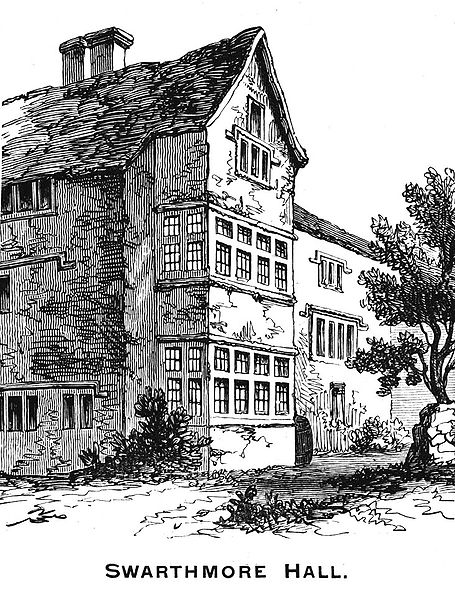
\includegraphics[width=0.20\textwidth]{./pics/swarthmore_hall.png}
\label{bild:swarthmoor} 
\end{floatingfigure}



Wir zogen durch Nottinghamshire nach Lineolnshire .....
Hier kam zu einer unserer Versammlungen ein Mann und erhob eine
falsche Anklage gegen mich; er verbreitete überall daö Gerücht, ich
habe gesagt, ich sei Christus-, was gänzlich falsch war. Al-? ich dann
nach Gainßborough kam, wo einer der Freunde auf dem Markt-
platz die Wahrheit verkündet hatte, fand ich die ganze Stadt und
alle Marktleute in Aufruhr. Jch ging inß Haus eineö Freunde?-,
und daß Volk drängte sich hinter mir drein, biz das Haus ganz
voll war von »Frommen«, Giferern und Pöbel; da kam jener
falsche Verleumder herein und klagte mich öffentlich vor allen an,
ich hätte gesagt, ich sei Christuß, und er habe Zeugen, es zu be-
weisen. Das brachte die Leute so in Wut, daß man Miihe hatte,
mich vor ihnen zu schützen. Da trieb mich der Geist dez Herrn
aus einen Tisch zu stehen und in der ewigen Kraft dez Herrn
den Leuten zu verkünden, daß Christuö in ihnen sei, etz sei denn,
daß sie Verdammte seien; und daß eß Christuö, die ewige Kraft
Gottes sei, welche jetzt auß mir zu ihnen rede, nicht ich sei Christus;
die Leute waren im allgemeinen befriedigt außer jenem »Frommen«
und einigen falschen Zeugen. Jch nannte diesen Ankläger Judaö,
und es trieb mich, ihm zu sagen, daß das Ende deö Judaß auch
das seine sein werde; solches- lasse ihm der Herr durch mich sagen.
Dez Herrn Macht kam über alle und beruhigte die Gemüter der
Leute und sie gingen in Frieden fort. Jener Judaß aber machte
sich davon und erhenkte sich und man steckte einen Pfahl in sein
Grab. Daraufhin erhoben die bösen Priester eine Verleumdung
gegen unö und streuten aus, ein Quäker habe sich erhenkt in
Lineolnshire. Diese Lüge ließen sie drucken und verbreiten und
hänften so Sünde auf Sünde. Mer wir und die Wahrheit wurden
nicht davon getroffen; denn jener war so wenig ein Quäker als
der Priester, der solcheß gedruckt hatte; vielmehr war eögeiner


% \picinclude{./050-059/p_s057.jpg} 
Christus in uns. Erkenntniz der Quükerischen Weltmisfion usw. 57
ihrer eigenen Leute. Aber trotz dieser argen Lüge, mit welcher der
Gegner beabsichtigthatte, unß zu verleumden und die Leute von
der von unß verkiindeten Wahrheit abzukehren, nahmen doch viele
in Lineolnshire daß Evangelium an, da sie von der ewigen Wahr-
heit überzeugt waren und sich zu Füßen deß himmlischen Herm
setzten ......
Wir zogen nun wieder .... über Warmßworth . . . Bably,
Doneaster .... nach Tickhill, wo an einem Ersten Tage die
Freunde der Gegend sich versammelten, und eß herrschte durch
Gottes Macht eine tiefe Zerknirschung in der Versammlung.
Jch verließ die Versammlung, da Gott mich trieb inß Turmhauß
zu gehen. Alß ich dorthin kam, fand ich den Priester und saft
alle Gemeindeältesten im Chor beisammen. Jch ging zu ihnen
und hub an zu ihnen zu reden, aber sie sielen sogleich über mich
her, und ein Priester nahm seine Bibel und schlug mich damit
inß Gesicht, so daß ich heftig blutete im Turmhauß; daß Volk
schrie: ,,Hinauß mit ihm auß der Kirche!« Und alß sie mich hinauß
gebracht hatten, prügelten sie mich und warfen mich zu Boden
und über eine Hecke; hernach schleppten sie mich durch ein Hauß
aus die Straße; sie warfen mich mit Steinen und schlugen mich,
während sie mich Vorwärtß tissect, so daß ich über und über mit
Kot beschmiert war. Sie nahmen mir den Hut, den ich nicht
mehr wieder bekam. Alß ich jedoch wieder auf den Füßen war,
verkündete ich ihnen daß Wort deß Lebenß und zeigte ihnen, wo-
hin ihre Lehre sie führe und wie sie daß Christentum entehrten. Nach
einer Weile ging ich wieder in die Versammlung zurück zu den
Freunden. Und alß die Priester und die Leute am Hause vorbei
kamen, ging ich mit einigen Freunden hinauß in den Hof und
redete zum Priester rmd den Leuten. Der Priester verhöhnte
unß und nannte unß ,,Quäker«. Aber die Macht deß Herrn
kam dermaßen über sie und daß Wort deß Lebenß wurde ihnen
so überzeugend und eindringlich verkündet, daß der Priester selber
zu zittern begann und einer sagte: »seht wie der Priester zittert
und bebt, er wird auch ein Quäker«. Alß die Versammlung zu
Ende war, gingen die Freunde sort, und ich ging, ohne Hut,
nach Balby, etwa sieben bis acht Meilen weit. Die Freunde
wurden an dem Tage dergestalt von dem Priester und seinen
Anhängern mißhandelt, daß einige Friedenßrichter, alß sie davon
hörten, kamen und ein Verhör in dieser Stadt anstellten, um


% \picinclude{./050-059/p_s058.jpg} 
58 Kapitel lt.
die Sache zu untersuchen. Der, welcher mich blutig geschlagen
hatte, fürchtete, man haue ihm die Hand ab; aber ich vergab
ihm und klagte nicht gegen ihn.
Zu Anfang deö Jahres- 1652 regte sich heftiger Widerstand
gegen die Wahrheit und die Freunde, bei Priestern und Volk
und bei etlichen der Behörden in Yorkshire, so daß der Priester
von Warmöworth sich einen Verhaftbefehl gegen mich und Thomaß
Aldam verschaffte, der in allen Teilen im westlichen Bezirk York-
shireö auögeführt werden konnte. Zu dieser Zeit hatte ich ein
Gesicht von einem Bären und zwei großen, riesigen Hunden, und
wie ich bei ihnen vorbei mußte, ohne daß sie mir ein-aß tun
konnten. Und so geschah es; denn der Konstabler ergriff Thomaß
Aldam und brachte ihn nach York; und ich ging ein großeö Stück
Wegß mit ihm. Der Kanstabler hatte auch einen Verhaftbesehl
gegen mich und sagte zu mir: er sehe mich schon, aber er möge
nicht einen der ihm fremd sei, behelligen; Thomaß Aldam sei
eben sein Nachbar. Also hielt ihn die Kraft des Herrn, daß er
mich in Ruhe ließ. Wir kamen in die Wohnung deö Leutnant
Roper, wo wir eine große Versammlung hatten, worunter viele
angesehene Leute waren; die Wahrheit wurde mächtig kund
unter ihnen und die Schrift herrlich erklärt, und die Gleichnisse
und Reden Jesu wurden außgelegt und die Kirche, wie sie in den
Tagen der Apostel war, und der Abfall von derselben. Die
Wahrheit gelangte zur Herrschaft an jenem Tage, so daß jene
angesehenen Leute alle zugestanden: ,,diese Anschauungen werden
sich über die ganze Erde aus-breiten«. Dieser Versammlung
wohnten auch Jametz Naylor, Thomas Goodyear und William
Dewßbury, die das Jahr vorher gewonnen worden waren, sowie
Richard Farne-worth bei. Der Konstabler blieb mit Thomaß
Aldam, bis die Versammlung auö war, darm ging er mit ihm
nach dem Gefängnis in York; mich aber ließ er in Ruhe ....
Darnach kam ich nach Hightown, wo eine Fran wohnte, die
kurz vorher bekehrt worden war. Wir gingen in ihr Haus und.
hielten eine Versammlung, und die Leute versammelten sich, und
wir verkiindeten ihnen die Wahrheit und wirkten für den Herrn
unter ihnen, und sie gingen in Frieden wieder von dannen.
Aber ez war dort eine Witwe, namens Green, von böser Ge-
sinnung; diese ging zu einem sogenannten ,,Herrn« (cieutleman)
und verklagte unö bei ihm, obwohl er kein Beamter war. Am


% \picinclude{./050-059/p_s059.jpg} 
Christus in uns. Erkenntnis der Quäkerischen Weltmission usw. 59
nächsten Morgen sandten wir dem Priester einige Fragen. Alö
wir gerade fort gehen wollten, kamen einige, die sich zu une
hielten, gerannt und sagten, dieser Mörder habe sein Schwert
für unß geschärst und komme mit demselben gegen unß. Da wir
gerade fort gingen, oerfehlten wir ihn. Aber kaum waren wir
sort, so kam er in das Haus, in dem wir gewesen waren, und
es hieß allgemein, wenn wir nicht fort gewesen wären, so wären
wir ermordet worden. Wir brachten die Nacht im Walde zu
und wurden ganz durchnäßt, denn es regnete stark. Am Morgen
trieb es- mich roicher in die Stadt zurück, wo sie unß außfiihrlich
über jenen Bösewicht berichteten.
Von da gingen wir nach Vradsord, wo wir Richard Farnß-
worth trafen, von dem wir unö kurz vorher getrennt hatten.
A18 wir in sein Haus kamen, setzte man unß Fleisch nor, aber alß
. ich anfangen wollte, geschah daß Wort deö Herrn an mich: »Jß nicht
Brot bei einem Neidischen« (Spr. 23, 6). Sogleich stand ich
vom Tische auf und aß nicht;3. Die Frau war eine Baptistin.
Nachdem ich die ganze Familie ermahnt hatte, sich zum Herrn
zu bekehren und auf seine Lehre in ihren Herzen zu merken,
gingen wir von dannen ......
Unterwegs; kamen wir zu einem großen Hügel, genannt Pend-
lehill; und der Herr trieb mich, aus denselben hinauf zu gehen,
maß ich mit großer Anstrengung tat, denn er war sehr steil und
hoch. Alö ich oben ankam, blickte ich auf daß Meer, das Lan-
cashire umspült. Von diesem Hügel aut:-’ zeigte mir der Herr
die Orte, wo ihm ein großetz Volk sollte gesammelt werden.
Beim Hinuntergehen sand ich eine Wasserquelle am Abhang
dez Hiigelß, auß der ich mich ersrischte, denn ich hatte in den
letzten Tagen nur wenig gegessen und getrunken. Am Abend
kamen wir zu einer Herberge .... und hier ließ mich der
Herr ein Gesicht sehen: eine große Schar in weißen Kleidern
am Ufer eines Flusses, die zum Herrn kamen, und der Ort, den
ich sah, war bei Wen?-leydale und Sedbergh. . .
Wir zogen durch die Daleö . . . nach Dent .... Hier ging
ich zu Richard Robinson und redete von der Wahrheit zu ihm:
Ju einer Versammlung bei Frieden?-richter Benson traf ich Leute,
die sich vom öffentlichen Gotteödienst lozgesagt hatten. Dies
war der Ort, den ich gesehen, wo eine Schar in weißen Kleidern
daher kam. GS war eine große Versammlung, und die meisten



\picinclude{./060-069/p_s060.jpg} 
\picinclude{./060-069/p_s061.jpg} 
\picinclude{./060-069/p_s062.jpg} 
\picinclude{./060-069/p_s063.jpg} 
\picinclude{./060-069/p_s064.jpg} 
\picinclude{./060-069/p_s065.jpg} 
\picinclude{./060-069/p_s066.jpg} 
\picinclude{./060-069/p_s067.jpg} 
\picinclude{./060-069/p_s068.jpg} 
\picinclude{./060-069/p_s069.jpg} 


% \picinclude{./070-079/p_s070.jpg} 
Gide der Zeugen gänzlich falsch seien, und daß ich nichts der-
gleichen geäußert habe .... Oberst West, der ale Friedenörichter
der Gegend hier war, schenkte dieser Auzsage Gehör; und
nachdem er vorher lange krank gewesen war, bekannte er nun,
heute habe ihn der Herr geheilt, und fügte bei, er habe noch nie
so viele gute Menschen und liebe Gesichter beisammen gesehen in
seinem ganzen Leben. Und darauf wandte er sich zu mir und
sagte vor allen: ,,George, wenn du irgend etwas zu den Leuten
zu sagen hast, so tue ee ungehindert«. GS trieb mich zu reden,
worauf der Priester, der gegen mich geredet hatte, sich davon
machte. Jch sühlte mich getrieben zu erklären, daß: ,,die heilige
Schrift vom Geist Gotteß eingegeben sei, und daß alle zuerst
den Geist Gottes in ihrem Jnnern erkennen müssen, durch den
sie Gott und Ehristuö, von denen die Propheten und Apostel
lernten, erkennen können; und durch diesen selben Geist werden
sie dann auch die heilige Schrift verstehen. Denn wie der Geist
Gottes in denen war, die die Schrift geschrieben, so muß derselbe
Geist Gottes auch in denen sein, die die Schrift verstehen wollen;
durch diesen Geist haben sie allein Gemeinschaft mit dem Vater
und dem Sohne und mit der Schrift und untereinander; ohne
diesen Geist aber kann man weder Gott noch Christuß, noch die
Schrift kennen, noch Gemeinschaft untereinander haben«. Kaum
hatte ich solches gesagt, so brachen eine Anzahl Priester hinter
mir los und einer, Jackuö, behauptete unter anderm, der
Buchstabe und der Geist seien unzertrennlich. Darauf erwiderte
ich: ,,dann hat also jeder, der den Buchstaben hat, auch den
Geist, und kann also den Geist mit dem Buchstaben der Schrift
kausen«. Richter Fell und Hauptmann West machten den Pnestcttt
Vorstellungen über diesen ofsenkundigen Irrtum und sagten ihnen,
daß sie ja dann ihrer Ansicht nach den Geist in der Tasche herum
tragen könnten, wie den Buchstaben. Als die Priester sich besiegt
sahen, kehrten sie ihre Wut gegen die Friedenörichter, weil sie
ihre Rache gegen mich nicht stillen konnten. A18 die Friedens-
richter sahen, daß die Zeugen nicht mit einander übereinstimmten,
und daß sie eigentlich nur gewonnen worden waren, um der
Bosheit der Priester zu dienen, und daß alle ihre Anklagen nicht
gültig waren vor dem Gesetz, sprachen sie mich frei .... Jch
war also vor offenem Gerichtshof von allen falschen Anschul-
digungen gereinigt, und viele priesen Gott darüber; denn es war


% \picinclude{./070-079/p_s071.jpg} 
Fox der hexerei verdächtigt. Falsche Offenbarungen usw. 71.
ein Tag der Freude für viele. Friedenßrichter Benson von West-
morland 1) und Major Ripan von Lancaster wurden gewonnen.
GS war ein Tag deS Heilö für Hunderte; denn der Herr Jesus
Christus, der ,,Weg zum Vater«, und der ,,Lehrer der umsonst
lehrt--, wurden gepriesen, und sein ewige-8 Evangelium wurde ge-
Hpredigt und das Leben wurde verkündet, trotz allen diesen Priestern
und gewinnsüchtigen Predigern. Der Herr öffnete an dem Tage
vielen den Mund, daß sie den Priestern Vorstellungen machten
in den Herbergen und in den Straßen, so daß sie wie ein altes
morscheö Gebäude zerfielen; und es hieß allgemein, die Quäker
hätten gesiegt, und die Priester seien unterlegen. Unter andern
war auch Thoma-3 Briggs an diesem Tage gewonnen worden. Gr
war ein Gegner der Freunde gewesen, und als er einmal mit
John Lawson, einem Freund, über die Vollkommenheit geredet hatte,
rief er: ,,waZ, du glaubst an V-ollkommenheit?« und gab ihm dabei
eine Ohrfeige. Dieser Thomaß Briggß 2) wurde an diesem Tage
gewonnen und trat gegen seinen eigenenen Priester Jackuz auf; er
wurde nachher ein treuer Diener dez Evangeliums und blieb es
biz anö Ende seiner Tage ......


%%%%%%%%%%%%%%%%%%% Kapitel 6. %%%%%%%%%%%%%%%%%%%%%%%%%%%%%%

\chapter[Falsche Offenbarungen]{Falsche Offenbarungen}

\begin{center}
\textbf{Fox der Hexerei verdächtigt. Falsche Offenbarungen 
bei Freunden. Gefangenschaft in Carlisle.}
\end{center}

.... Von Lancaster ging ich zu Friedenßrichter West; Richard
Hubberthorn begleitete mich. Da wir den Weg und die Gefahr
der Sandbänke nicht kannten, ritten wir über eine Stelle, über
die, wie wir nachher erfuhren, noch nie jemand zuvor geritten
war. Wir ließen unsre Pferde über sehr gefährliche Stellen
schwimmen. Alß wir ankamen, fragte untz Friedenzrichter West,
ob wir nicht zwei Männer hätten über die Sandbänke reiten
sehen. »Jch werde«, fügte er bei, ,,über kurzem ihre Kleider
1) Getoase Benson war früher Oberst in der Armee gewesen und nun
Friedenstichter in Kendal.
2) Thoma-3 Briggs, der bisher ein eisriger Verfolger der Freunde ge-
wesen, wurde nun ihr Anhiiuger und ein bedeutender Prediger. E: hatte eine
große Gabe der Überzeugung. Er begleitete Fox aus vielen Reisen.


% \picinclude{./070-079/p_s072.jpg} 
haben, denn sie sind sicher ertrunken, und ich bin der Leichen-
schauer«. A15 wir ihm nun sagten, daß wir diese Männer seien,
da wunderte er sich sehr und wollte kaum glauben, daß wir nicht
ertrunken seien. Und die Priester und »Fromen« benützten es, um
daß Gerücht über mich zu verbreiten, ich könne nicht ertrinken mid
man könne mich nicht bluten machen, also sei ich ein Zauberer.
EZ war in der Tat oft vorgekommen, daß ich kaum blutete, wenn
sie mich mit ihren Stöcken schlugen und meinen Leib arg miß-
handelten. Alle diese Verleumdungen kitmmerten mich nicht um
meiner selbst willen; nur um die Wahrheit war mir bange,
gegen die sie mit solchen Mitteln die Leute einzunehmen suchten;
denn ich dachte daran, wie ihre verräterischen Vorfahren den
Hau?-herrn Beelzebub genannt hatten (Matth. 10, 25), und so
konnten ja diese von dem Leben und der Kraft Gotteß abge-
fallenen Christen mit seinem Samen nicht anderßz verfahren. Aber
die Kraft dez Herrn erhob mich über ihre Verläumderischen Zungen
und ihre blutige, mörderische Gesinnung; sie waren selber behext
und darum konnten sie nicht zu Gott und Christuö kommen.
Von Frieden?-richter West ging ich nach Swarthmore, wo
die Kraft deß Herrn die Verfolger niederhielt. ES trieb mich,
verschiedene Briefe von hier aus an die Magistrate, Priester und
,,Frommen« der Umgegend, die sich früher an den Verfolgtmgen
beteiligt hatten, zu schreiben. . . und hernach trieb es mich, an
die Leute in Uloerstone im allgemeinen einen Mahnbrief zu
schreiben ....
Unter den eifrigsten Zuhörern und Nachsolgern dez Priester-?
Lampitt vonU10erstone war ein Adam Sands, ein sehr schlechter,
verdorbener Mensch, der gerne die Wahrheit und ihre Anhänger
vernichtet hätte, wenn er gekonnt hätte. GZ trieb mich, an diesen
also zu schreiben:
,,Adam Sands!
Jch wende mich an daß Licht in deinem Gewissen, du Kind
des Teuselö, du Feind der Gerechtigkeit. Der Herr wird dich
darniederwerfen, wenn du schon eine Zeitlang jetzt herrschest. Die
Strafe Gottes muß dich treffen, der du dich in deiner Bosheit gegen
die reine Wahrheit Gotteß verhärtest. Durch die reine Wahrheit
Gotteö, die du verfolgest und der du widerstrebst, wirst du ver-
nichtet werden; sie ist ewig und schließt auch dich ein; du wirst
in dem Lichte, daß du verachteft, gesehen und in demselben ver-


% \picinclude{./070-079/p_s073.jpg} 
Fox der Hexerei verdächtigt. Falsche Osseubarungen nsw. 73
dümmt, du in deinem tierischen Wesen und dein Weib in seiner
Heuchelei; euer Morden der Gerechtigkeit wird erkannt werden;
das Licht in deinem Gewissen wird dir das, was ich dir hier
schreibe, bezeugen und wird dich erkennen lassen, daß du nicht
aus Gott geboren bist, sondern daß du sem von der Wahrheit
noch in einem tierischen Wesen bist. Wenn je einmal deine Augen
die ausgehen werden und du bereust, so wirst du sehen, daß ich
ein Freund deiner Seele bin und dein ewiges Heil will.
G. F.«
Dieser Adam Sands kam später elendiglich um .....
Ich ging nach Swarthmore zurück. Ich hatte große Offen-
banmgen vom Herm, nicht nur uber göttliche Dinge, sondern
auch über äußere, die die Regierung betrafen. Eines Tages,
als ich im Gerichtssaal Richter Fell und Friedensrichter Benson
über die jüngsten Ereignisse sprechen hörte und oom Parlament,
dasidamals tagte, und das man das ,,lange Parlament« nannte,
trieb es mich, ihnen zu sagen, daß, ehe zwei Wochen um seien,
das Parlament aufgelöst und der Redner von seinem Stuhl herunter
gerissen sein werde. Und als nach zwei Wochen Friedensrichter
Benson wieder kam, sagte er zu Richter Fell, jetzt sehe er, daß
George Fox ein wahrer Prophet sei: Oliver Cromwell habe das
Parlament ausgelöst! (20. April 1653.)
Um diese Zeit fastete ich etwa 10 Tage lang, weil mein
Geist um der Wahrheit willen schwer heimgesucht war; denn
James Milner und Richard Näher hatten Einbildungen und viele
machten es ihnen nach. Dieser James Milner und einige seiner
Anhänger hatten zuerst wahre Offenbarungen; aber da sie in
Hochmut und Selbstiiberhebung gerieten, irrten sie von der
Wahrheit ab. Der Herr trieb mich, zu ihnen zu gehen und ihnen
Ihre Verirrungen vorzustellen; und sie kamen dazu, ihre Torheit
emzusehen, und gaben sie auf und kamen aus den Weg der
Wahrheit zurück. Darauf begab ich mich in eine Versammlung
M Arn-Side, der Richard Myer beiwohnte; er hatte lange einen
lshmen Arm gehabt. Der Herr trieb mich, ihm vor allen An-
wesenden zu sagen: ,,Stehe auf!« und er stand aus und streckte
seinen Arm, der so lange lahm gewesen war, aus und sagte:
»Wisset, alle ihr Leute, daß ich heute geheilt worden bin.« Seine
Eltern wollten es kaum glauben, und als die Versammlung
vorbei war, nahmen sie ihn aus die Seite und zogen ihm sein


% \picinclude{./070-079/p_s074.jpg} 
Wamß au?-; da sahen sie, daß ez wahr sei. Er kam bald darauf
in eine Versammlung in Swarthmore und berichtete da, wie
der Herr ihn geheilt habe. Dornach befahl ihm der Herr, nach
York zu gehen in seinem Auftrag; aber er gehorchte dem Herrn
nicht; und der Herr schlug ihn abermals, daß er etwa dreiviertel
Jahr daraus starb ....
Um diese Zeit wurde Anthony Pearson X), der ein Gegner der
Freunde gewesen war, gewonnen. Er kam nach Swarthmore,
und da ich gerade dort bei Oberst West war, holte man mich.
Oberst West sagte: ,,Geht, Fox, denn Jhr könnt dem Mann zu
großem Nutzen gereichen«—. Also ging ich, und die Kraft deß
Herrn ergriff ihn.
Um diese Zeit tat der Herr auch etlichen den Mund auf,
daß sie den Priestern und dem Volk die Wahrheit verkündeten,
und viele wurden de-zwegen inö Gefängniö geworfen. Jch ging
nun nach Cumberland, wo Anthony Pearson, seine Frau und
mehrere Freunde mich nach Bootle begleiteten; Anthony Pearson
verließ uns dann, um zur Gerichtßsitzung nach Carlißle zu gehen;
denn er war Frieden?-richter in drei Grafschasten. An einem
Ersten Tage ging ich ins Turmhauö von Vootle, und als der
Priester fertig war, sing ich an zu reden. Aber die Leute waren
sehr unverschämt und prügelten mich im Hofe. Einer gab mir
einen starken Schlag aus daß Handgelenk, sodaß man allgemein
glaubte, er hätte meine Hand in Stücke geschlagen. Der Kon-
stabler hätte gem den Frieden wieder hergestellt und einige, die
mich geschlagen, eingesteckt; aber ich ließ es nicht zu. Nachdem
ich zu ihnen geredet, ging ich nach der Wohnung dez Joseph
Nicolson und der Konstabler begleitete mich, um mich vor der
Menge zu schützen.
Am Nachmittag hatte der Priester einen andern Priester
kommen lassen, einen sehr angesehenen Mann auß London. Ehe
ich inö Turmhautz eintrat, saß ich eine Weile auf dem Platz davor
und einige Freunde mit mir; aber die Freunde wurden getrieben, ins
Turmhauz zu gehen, und ich ging ihnen nach. Der Londoner
Priester brachte in seiner Predigt alle erdenklichen Schriftftellen
von falschen Propheten rmd Antichristen und wandte sie auf unö
an. Aber alß er geendet, nahm ich alle die Schriftstellen noch
1) Friedenörichtev Pearson wurde ,,bekehrt, als er auf dem Richterstuhl saß«.


% \picinclude{./070-079/p_s075.jpg} 
Fox der Hexerei verdächtigt. Falsche Qssenbarungen usw. 75
einmal durch und kehrte sie gegen ihn. Darauf überfielen mich
die Anwesenden, aber der Konstabler befahl ihnen Ruhe. Nun
wurde der Priester zornig und erklärte, ich dürfe nicht an diesem
Ort reden. Jch erklärte ihm, er habe auch seine Stunde zum
Predigen gehabt, nun sei seine Zeit um, und nun dürfe ich so
gut die meine reden wie er, denn er sei auch nur ein Fremder
hier. Und ich öffnete ihnen die Schrift und zeigte ihnen, daß
diese Stellen, die von falschen Propheten, Betrügern und Anti-
christen reden, sie und ihreögleichen betrefse und alle, die in ihren
Fußstapfen gehen und die gleichen Früchte hervorbringen wie sie;
und nicht uns-, denn man könne uns solche Dinge nicht nach-
sagen. Jch zeigte ihnen, wie sie nicht in den Fußstapfen der
wahren Propheten und Apostel seien und wies ihnen an den
Früchten, die sie hervorbringen, nach, daß sie etz seien, von denen
die Schriftstellen handeln und nicht wir. Und ich verkündete ihnen
die Wahrheit und daß Wort deß Lebenß und wies sie aus Christ-.13,
ihren Lehrer. Alletz war ruhig während ich redete; aber alß ich
geeudet hatte und hinaus kam, waren die Priester in einer solchen
Wut, daß ihr Mund gegen mich schäumte. Der Priester des
Orts redete auf dem Turmplatz zu den Leuten und sagte ihnen:
,,Dieser Mensch hat in Laneashire alle rechtfchassenen Männer
und Frauen für sich zu gewinnen gewußt, und nun will er hier
da?-selbe tun.« Jch erwiderte ihm: ,,WaS bleibt dann für die
Priester übrig, außer solchen wie sie selber sind? Denn wenn es
die Rechtschafsenen sind, die sich zur Wahrheit bekehren und sie
aufnehmen und sich zu Christuß bekehren, so sind es die Schlechten,
die dir und deineßgleichen folgen! Etliche suchten für ihren Priester
einzutreten, und für das Zehntenwesen; aber ich sagte ihnen, sie
täten besser, für Christus einzutreten, der den Zehntenpriestern
und dem Zehntenwesen ein Ende machte und der seine Jünger
aussandte mit der Weisung: ,,untsonst zu geben, wa-3 sie umsonst
empfangen hatten«. Und des-Z Herrn Macht kam über alle und brachte
sie zum Schweigen und hielt die Schreier zurück, daß sie den Unfug,
den sie planten, nicht ausführen konnten. A13 ich zu Joseph
Nieolson zurück kam, entdeckte ich ein großeß Loch in meinem
Rock, daß von einem großen Messerstich herrührte; aber ez war
nicht tiefer alö der Rock gegangen, denn der Herr hatte ihre
Ubeltat vereitelt .....
Darnach ging ich in ein Dorf, und eine große Schar be-


% \picinclude{./070-079/p_s076.jpg} 
gleitete mich. Während ich in einem mit Leuten ganz gefüllten
Hauö das- Wort des Lebenö verkündete, gewahrte ich eine Frau,
die, wie ich gleich merkte, einen unsauberen Geist hatte. Der
Herr trieb mich, ernstlich mit ihr zu reden und ihr zu sagen, sie
sei unter dem Einfluß eineö unsauberen Geisteö; hierauf verließ
sie daß Zimmer. Weil ich fremd war an diesem Orte und die
äußeren Verhältnisse der Frau nicht kannte, wanderten sich die
Leute sehr und sagten mir nachher, ich hätte etwas Merkwiirdigeß
entdeckt; denn diese Frau sei wirklich lange als eine schlechte
Person bekannt gewesen. Der Herr hatte mir die Gabe der
Unterscheidung gegeben, durch welche ich den Zustand und die
Verfassung der Leute ost erkannte und die Geister prüfen konnte
denn nicht lange vorher, alö ich in eine Versammlung ging, sah
ich auf dem Felde einige Frauen, bei denen ich einen unsauberen
Geist erkannte; und etz trieb mich, von meinem Wege ab zu ihnen
zu gehen und ihnen ihren Zustand aufzudecken. Ein andermal
kam eine in die Versammlung in Swarthmore, und etz trieb mich,
ernstlich mit ihr zu reden und zu sagen, sie stehe unter der Macht
eines bösen Geisteö; und die Leute sagten nachher, etz sei daß
allgemein von ihr bekannt. Gin andermal kam eine andere Frau
und stand in einiger Entfernung von mir, und es trieb mich zu
ihr zu gehen und zu sagen: »Du bist eine Hure gewesen«; denn
ich erkannte den Zustand und daß Leben dieser Frau; sie antwortete
mir, es gebe viele, die ihr ihre äußern Sünden nennen können,
aber ihre inwendigen habe ihr noch niemand sagen können; daraus
sagte ich ihr, ihr Herz tue nicht recht vor dem Herrn, rmd
aus dem inwendigen komme das auöwendige; diese Frau wurde
nachher von der Wahrheit dez Herrn überzeugt und schloß sich
den Freunden an .....
Wir gingen nun nach Earliöle ..... An einem Markttage
ging ich aus den Markt. Die Magistrate hatten Drohungen er-
gehen lassen und ihre Leute geschickt; und ihre Frauen hatten
gesagt, wenn ich komme, so reißen sie mir die Haare auö, und
die Schutzleute sollten mich nur sestnehmen. Aber ich ging dennoch
auf den Platz, im Gehorsam gegen den Herrn, und verkündete
ihnen dort, daß der Tag des Herm über all ihr betrügerischeö
Tun und ihre betriigerische Ware komme; und sie sollten sich alle
abwenden von ihrem Beträgen und Überlisten und sich an Ja
und Nein halten und einander die Wahrheit sagen; dann komme


% \picinclude{./070-079/p_s077.jpg} 
Fox der Hexerei verdächtigt. Falsche Offenbarungen usw. 77
die Kraft und die Wahrheit des Herrn zu ihnen. Nachdem ich
ihnen so das Wort des Lebens verkündet hatte, in einem Ge-
dränge, das zu groß gewesen war, als daß die Schutzleute und
die Weiber der Magistrate zu mir hätten gelangen können, zog
ich ruhig weiter. Viele Soldaten und andere kamen zu mir und
einige Baptisten, die heftige Streiter waren; unter diesen war
auch ein Helfer, ein böser Mann, der, als er die Kraft des Herrn
verspürte, aufschrie vor Zorn, worauf ich meine Augen auf ihn
heftete und ernstlich zu ihm redete in der Kraft des Herm; und
er schrie: ,,Durchbohre mich nicht so mit deinen Augen! wende
deine Augen ab von mir«.
Am folgenden Ersten Tage ging ich ins Turmhaus, und
nachdem der Priester geendigt hatte, predigte ich den Leuten
die Wahrheit und das Wort des Lebens. Der Priester entfernte
sich und man wollte mich aus dem Turmhaus jagen. Aber ich
verkündete den Weg des Herrn weiter unter ihnen und sagte:
,,ich komme, euch das Wort des Lebens und der Seligkeit zu ver-
künden«. Die Macht des Herrn tat sich mächtig kund unter
ihnen, so daß sie zitterten und bebten, und meinten, das Turm-
haus schwanke, und einige meinten, es werde auf ihre Köpfe fallen;
die Weiber der Magistrate rasten und suchten mit aller Gewalt,
an mich heran zu kommen; aber die Soldaten und die Freunde
umringten mich. Zuletzt kam der ganze Pöbel der Stadt ins
Turmhaus, mit Stöcken und Steinen und schrie: ,,nieder mit
diesen rundköpfigen Schuften!« und warfen mir Steine an.
Hierauf schickte der Statthalter Soldaten ins Turmhaus, um
Ruhe zu schaffen unter den Leuten; mich nahmen sie freundlich
bei der Hand und hießen mich mit ihnen kommen. Als wir
auf die Straße kamen, war die Stadt in Aufrrchr, und einige
dieser Soldaten kamen ins Gefängnis, weil sie sich meiner ange-
nommen hatten, gegen die Leute aus der Stadt. Gin Leutnant,
der belehrt worden war, nahm mich in sein Haus, wo eine Vap-
tistenversammlung war; auch Freunde kamen dazu, und wir hatten
eine sehr ruhige Versammlung; sie hörten das Wort des Lebens
gerne, und viele nahmen es auf. Am folgenden Tage, als die
Magistrate im Stadthaus versammelt waren, ließen sie mich vor
sie bringen. Jch war eben im Haus eines Baptisten; als ich
von dem Befehl hörte, ging ich nach dem Stadthaus hinauf, wo
viel Pöbel versammelt war, der allerlei falsche Dinge über mich


% \picinclude{./070-079/p_s078.jpg} 
auögesagt hatte. Ich hatte eine lange Unterredung mit den
Magistraten, worin ich auseinandersetzte, waz für Früchte die
Predigten ihrer Priester bringen, und wie wenig Christentum darin
sei; und ich sagte ihnen, daß sie zwar alß große »Fromme«
gelten, — sie waren Preßbhterianer und Jndependenten — aber
eben nicht im Besitz ihrer Frömmigkeit seien. Nach einem langen
Verhör verurteilten sie mich zum Gefängniö, alß Gottes-lästerer,
Ketzer und Verführer, obgleich sie mich gerechter Weise keines
dieser Dinge beschuldigen konnten. EZ waren zwei Kerkermeister
im Kerker von Carliöle, ein oberer und ein unterer, die auß-
sahen wie zwei große Värensührer. A15 ich gebracht wurde,
führte mich der Oberkerkermeister in ein großeß Zimmer und sagte
mir, ich könne hier haben, was ich wolle; aber ich erwiderte
ihm, er solle kein Geld von mir erwarten, denn ich werde weder
in einem seiner Betten schlafen, noch von seinen Speisen essen,
woraus er mich in ein anderes Gemach führte, wo ich nach einiger
Zeit etwas zum drauf liegen erhielt. Hier lag ich gefangen biß-
zur Zeit der Gerichtösitzung, wo ich, wie es- allgemein hieß, er-
henkt werde. Der Oberscherifs Wilfrid Lawson, hetzte sie auf,
mich zu töten, und sagte, er wolle mich selbst biß zu meiner Hin-
richtung bewachen. Sie waren sehr streng und setzten drei Muske-
tiere zu meiner Wache, einen vor meine Türe, einen anderen
unten an die Treppe und einen dritten vor die Haustüre, und
sie ließen niemand zu mir, außer um mir das nötigste zu bringen.
Dez Nachts brachten sie Priester zu mir, oft erst um zehn Uhr,
die schrecklich roh und teuflisch waren. GS gab eine Rotte von
schottischen Priestern, Preßbyterianer, zusammengesetzt auö Neid
tmd Bo?-heit, die nicht »geschickt waren, göttliche Dinge zu reden«
und sehr schmutzige Reden führten. Aber der Herr verlieh mir
durch seine Kraft die Herrschaft über sie alle, so daß sie erkannten,
in welchem Geist sie waren und maß sie für Früchte brachten.
Auch angesehene sogenannte ,,Damen« (lmtjez) kamen, um den
Mann zu sehen, von dem es hieß, er müsse sterben. Während
die Richter und Räte miteinander berieten, auf welche Art ich
sterben solle, vereitelte der Herr in Unerwarteter Weise ihren
Anschlag, indem der Anwalt einen Einwand verbrachte, der
alle ihre Absichten über den Haufen warf, so daß sie keine
Macht mehr hatten, mich vor Gericht zu bringen .....
Nachdem die Richter die Stadt verlassen hatten, erhielt der


% \picinclude{./070-079/p_s079.jpg} 
Fox der Hexerei verdächtigt. Falsche Ossenbarungen usw. 79
Kerkermeister Befehl, mich in den untersten Kerker zu den Straßen-
räubern, Dieben und Mördern zu werfen, obgleich ich schon vor-
her in sehr strengem Gewahrsam gewesen war. Jch kam nun
an einen gräulichen, schmutzigen Ort, wo nicht einmal ein Abtritt
war, Amd Frauen und Männer in unziemlicher Weise zusammen-
gesperrt waren, und die Gefangenen waren voll Läuse, so daß eine
Frau fast davon aufgesressen wurde; aber so schlecht auch der
Ort war, so kamen doch die Gefangenen alle dazu, mir zugetan
und ganz nachgiebig zu werden, und etliche wurden von der Wahr-
heit bekehrt, wie dieß bei Zöllnern und Huren zu allen Zeiten
geschehen, so daß sie jeden Priester, der anß Gitter kam, um mit
ihnen zu diöputieren, zu Schanden machen konnten. Der Kerker-
meister war sehr hart und der Unterkerkermeister roh gegen mich und
gegen die Freunde, die zu mir kamen. Gr schlug oft Freunde,
die nur anß Gitter kamen, um mich zu sehen, mit einem großen
Knüttel. Jch konnte am Gitter hinaus steigen, um zuweilen etwas
Fleisch herein zu langen, was ihn schrecklich böß machte. Einmal
überkam ihn ein solcher Zorn, daß er mich mit einem Kniittel
durchprügelte und dazu schrie: ,,komm vom Fenster weg!« obschon
ich gerade damals nicht dran war. Während er mich schlug,
—kam es in der Kraft des Herrn über mich, zu singen, maß ihn
noch wütender machte. Esr holte einen Geigenspieler und ließ
ihn vor mir spielen, weil er meinte, mich damit zu verdrießen.
Aber während seinem Spiel kam eZ über mich, in Gottes ewiger
Kraft zu singen, und meine Stimme übertäubte den Lärm des
Geigerö, waö ihn so oerwirrte, daß er das Spielen aufgab und
sich daoonmachte.
Richter Vensontz Frau fühlte sich getrieben, mich zu besuchen,
und kein anderes- Fleisch zu essen, al-3 von dem, daö man mir
an die Kerkertür brachte. Später wurde sie selbst in York ins
Gesängniß getan, während sie schwanger war, weil sie einem
Priester widersprochen hatte, und man gestattete ihr nicht, aus
dem Gefängniö zu gehen zur Zeit ihrer Niederkunft; so gebar
sie im Kerker ein Kind. Sie war eine gläubige, gottselige Frau,
und blieb etz biö zu ihrem Tode.
Während meiner Gefangenschaft im Kerker zu Carliöle ver-
breitete sich daß Gerücht von meiner wahrscheinlicher! Hinrichttmg
überall hin. Alß sie im Parlament — ich glaube es wurde das
kleine Parlament genannt — hörten, es sollte in Carliöle ein


% 
% \picinclude{./080-089/p_s080.jpg} 
% \picinclude{./080-089/p_s081.jpg} 
% \picinclude{./080-089/p_s082.jpg} 
% \picinclude{./080-089/p_s083.jpg} 
% \picinclude{./080-089/p_s084.jpg} 
% \picinclude{./080-089/p_s085.jpg} 
% \picinclude{./080-089/p_s086.jpg} 
% \picinclude{./080-089/p_s087.jpg} 
% \picinclude{./080-089/p_s088.jpg} 
% \picinclude{./080-089/p_s089.jpg} 


% \picinclude{./090-099/p_s090.jpg} 
90 Kapitel 711.
,,Geh, George, geh nur,« so fürchtete ich, daß, wenn ich nicht
ginge, man sage, ich sei meinen Eltern ungehorsam; so ging ich,
und die übrigen Priester wollten daß Volk abhalten, aber es
gelang ihnen nicht, denn da alle uns- hören wollten, wurden wir
ganz umringt. Jch fragte den Priester, maß er zu sagen habe?
er antwortete, wenn er nicht aus dem rechten Wege sei, so sollte
ich für ihn beten; und wenn ich nicht auf dem rechten Wege sei,
so wollte er für mich beten; und er wolle mir oorsagen, was ich
für ihn beten solle. Ich erwiderte ihm: ,,eS scheint, daß du nicht
einmal weißt, ob du auf dem rechten Wege bist; ich aber weiß,
daß ich auf dem rechten Wege bin, Jesus Christus, in welchem
du nicht bist, und du wolltest mir vorsagen, wie ich zu beten
habe, und verwirfst doch daß Common-Prayerbook so gut wie ich,
und ich verwerfe dein Geplapper ebenfalls. So du willst, daß ich
nach etwas Hergesagtem für dich bete, heißt daß nicht, die Lehre
der Apostel mißachten und ihr Beten im Geist, der die Worte
eingibt?« Hier fingen die Leute an zu lachen; mich aber trieb
ez, weiter zu ihm zu reden. Nachdem ich ihm gesagt, was
mir zu sagen oblag, und daß ich, so Gott wolle, über acht Tage wieder
in der Stadt sein werde, gingen wir fort. Die Priester machten,
daß sie fort kamen und viele wurden gewonnen, denn die Kraft dez
Herrn kam über alle. Wenn sie schon meinten an diesem Tage
der Wahrheit geschadet zu haben, war doch mancher gewonnen
worden, und viele, die schon früher gewonnen worden, wurden durch
daß, was an jenem Tage geschehen, bestärkt, und etz gab den
Priestern einen Stoß. Mein Vater, obgleich er ein Anhänger der
Priester war, war so befriedigt, daß er mit seinem Stock auf die
Erde schlug und sagte: »wahrlich, ich sehe, daß wer willenß ist,
bei der Wahrheit zu bleiben, dem wird sie durchhelsen« .....
Darauf zog ich wieder umher und hielt Versammlungen und
kam nach Swannington, wohin auch wieder Soldaten kamen;
aber die Versammlung war ruhig, die Macht Gotteö war
über allen, und die Soldaten störten mich nicht. Darauf ging
ich nach Leicester und Whetstone. Dahin kamen siebzehn Soldaten
auö Oberst Hackerß Regiment, mit ihrem Anführer, und führten
mich, gerade vor Beginn der Versammlung, hinweg, obgleich die
Freunde, die von allen möglichen Orten hergekommen waren,
schon anfingen sich zu versammeln. Ich sagte dem Vorgesetzten,
er solle wenigstenß die Freunde in Ruhe lassen, ich wolle für sie


% \picinclude{./090-099/p_s091.jpg} 
Kämpfe mit schwärmerischen Ranters und zehutengierigen Priestern usw. 91
alle haften; so nahmen sie denn mich und ließen die andern in
Ruhe, ausgenommen Alexander Parken!) der mit mir kam. Am
Abend brachten sie mich vor Oberst Hacker; sein Major, seine
Hauptleute und viele seiner Leute waren zugegen und wir gaben
auöfiihrlich Auskunft über die Priester und über die Versammlungen,
denn ez ging damals gerade daß Gerücht von einer Verschwörung
gegen Oliver Eromwell. Jch hatte lange Grörterungen über das
Licht Christi, daß einen jeden, der in die Welt kommt, erleuchtet
(Joh. 1, 9). Oberst Hacker fragte, ob e-3 dieses Licht auß Ehristuß
gewesen sei, daß den Judaö dazu geführt habe, seinen Herrn zu
verraten und sich darnach zu erhängen? Jch sagte ihm: ,,nein,
das war der Geist der Finsterniß, der Christuz und sein Licht
haßte.« Darauf sagte Hacker, ich solle nach Hause gehen und dort
bleiben, und nicht überall zu den Versammlungen gehen. Jch sagte
ihm, ich sei ein ganz harmloser Mensch und habe nichts mit Ver-
schwörungen zu tun, vielmehr verabscheue ich solcheß. Sein Sohn
Needham sagte: »Vater, dieser Mensch hat nun schon lange ge-
herrscht, eö ist Zeit, daß man ihn unschädlich mache.« q Jch fragte
ihn, ,,warum, was habe ich getan? oder wem habe ich je etwas
zu leide getan? ich bin in dieser Gegend geboren und aufge-
wachsen, wer kann mir irgend etwaß Böses nachsagen seit meiner
Kindheit?« Darauf fragte mich Oberst Hacker nochmals-, ob ich
nach Hause gehen wolle und dort bleiben? Ich antwortete ihm,
ich würde mich ja mit einem solchen Versprechen schuldig bekennen,
wenn ich nach Hause ginge und auö meinem Hause ein Gefängniß
machen wollte; und ginge ich dann doch zu den Versammlungen, so
würde ez heißen, ich sei dem Befehl ungehorsam. Jch erklärte
ihnen, ich gehe auf dee- Herrn Geheiß zu den Versammlungen,
darum könne ich mich ihren Vorschriften nicht fügen; aber wir
seien ein sriedlichez Volk. ,,Gut denn,« sagte Oberst Hacker, »ich will
euch zum Lord Protektor schicken, durch Hauptmann Drury, einen
aus seiner Leibgarde.« Die Nacht über wurde ich alß Gefangener
gehalten und am folgenden Morgen um sechö Uhr dem Haupt-
mann Drury übergeben. Ich wünschte vor dem Fortgehen noch
mit Oberst Hacker zu reden, er ließ mich vor sein Bett kommen und
drang sogleich wieder in mich, nach Hause zu gehen und keine
Versammlungen zu halten; ich erklärte ihm, ich könne mich dem
1) Alexander Parker, ein Mann von vornehmer Herkunft, reiste viel im
Dienst des Quäkertnmö und schrieb viele Bücher und Briefe zu seiner Verbreitung. NT


% \picinclude{./090-099/p_s092.jpg} 
92 Kapitel 711.
nicht fügen, sondern müsse meine Freiheit haben. ,,Dann,« sagte
er, ,,müßt ihr vor den Protektorcks Hierauf kniete ich an feinem
Bett nieder und betete zum Herm, ihm zu vergeben, denn er war
ein Pilatus, auch wenn er seine Hände gewaschen hätte; und ich
flehte zum Herrn, daß, wenn der Tag seiner Prüfung und Heim-
suchung komme, er sich dessen, was ich ihm gesagt, erinnern möge.
Gr war eben aufgehetzt von Priester Stephens und den andern
Priestern und ,,From1nen«, die darin ihre Bosheit ausließen, weil
sie mich durch ihr Argument nicht hatten überwinden können
und dem Geiste Gottes in mir nicht hatten widerstehen können;
darum hatten sie nun die Soldaten geschickt, um mich zu greifen.
Als später dieser Oberst Hacker im Gefängnis in London
war, wurde es ihm ein oder zwei Tage vor seiner Hinrichtung
in Erinnerung gebracht, wie er an den Unschuldigen gehandelt
hatte, und er gedachte daran und bekannte es Margaret Fell;
und es bedriickte ihn. Nun konnte sein Sohn, der damals
gesagt hatte, ich habe genug geherrscht, es sei Zeit, mich fort zu
schaffen, zusehen, wie sein Vater sottgeschasft wurde, als man ihn
erhängte in Tyburn.
Jch wurde nun von Hauptmann Drury als Gefangener von
Leieester fortgebracht. Als wir nach Harborough kamen, fragte
er mich, ob ich heimgehen wolle und 14 Tage dort bleiben? Er
versprach mir die Freiheit, wenn ich weder Versammlungen halten
noch zu solchen gehen wolle. Jch erwiderte ihm, ich könne nichts
dergleichen versprechen; er fragte und versuchte mich wiederholt
auf dem Wege in derselben Weise, und immer gab ich ihm die-
selbe Antwort. So brachte er mich nach London und quartierte
mich in Mermaid ein; unterwegs trieb es mich, die Leute zu J
warnen vor dem Tag des Herrn, der über sie kommen werde.,
Nachdem Hauptmann Drury mich untergebracht, verließ er mich
und ging zum Protektor, um Bericht über mich zu erstatten. Als
er zurückkam, sagte er, der Protektor verlange, daß ich kein
mörderisches Schwert gegen ihn oder die Regierung gebrauche,
und daß ich dies in beliebigen Worten schristlich erklären und mit
meiner Unterschrift versehen solle. Jch antwortete Hauptmann
Drury nur wenig; aber am nächsten Morgen trieb mich der Herr,«
ein Schreiben an den Protektor auszusetzen, in dem ich vor dem«
Angesicht Gottes des Herrn erklärte, daß ich das Tragen eines
mörderischen Schwertes oder irgend einer anderen äußeren Waffe


% \picinclude{./090-099/p_s093.jpg} 
Kämpfe mit schwiirmerischen Routers und zehntengierigen Priestern usw. 93
verabscheue, und daß ich von Gott gesandt sei, Zeugnis abzu-
legen gegen jegliche Gewaltttitigkeit und gegen die Werke der
Finsternis; und um die Leute von der Finsternis zum Licht zu
bringen und vom Kriegen und Streiten zum Evangelium des
Friedens. Nachdem ich geschrieben, was der Herr mir eingegeben
hatte, setzte ich meinen Namen darunter und übergab es Haupt-
mann Drury, damit er es Oliver Eromwell gebe, was er auch
tat. Rath einiger Zeit brachte mich Hauptmann Drury vor den
Protektor in Whitehall; es war an einem Morgen, ehe er ange-
kleidet war, und einer, namens Harvey, der sich auch eine Zeit
lang zu den Freunden gehalten hatte aber ungehorsam geworden
war, bediente ihn. Als ich eintrat, trieb es mich zu sagen:
,,Friede sei mit diesem Hause,« und ich ermahnte ihn, in der Furcht
Gottes zu bleiben, damit er Weisheit von ihm empfangen möge,
daß sie ihn leite; und daß er alle Dinge, die in seiner Hand
seien, zu Gottes Ehre regiere. Jch redete lange mit ihm über
die Wahrheit und über die Religion, er zeigte sich sehr verständig;
aber er sagte, wir zankten mit den Priestern, die er Diener Gottes
nannte. Jch entgegnete ihm, ich zanke nicht mit ihnen, sondern
sie mit mir und mit meinen Freunden. ,,Aber«, sagte ich, ,,wenn
wir die Propheten und Apostel anerkennen, so können wir solche
Lehrer, Propheten und Hirten, gegen welche die Propheten und
Christus auftraten, nicht gut heißen, sondem wir müssen auch
gegen sie auftreten, durch denselben Geist und dieselbe Krast.«
Ferner zeigte ich ihm, daß die Propheten, Christus und die
Apostel umsonst predigten und gegen die auftraten, welche es
nicht umsonst taten, sondern um schändlichen Gewinnes willen
und die um Geld wahrsagten und um Lohn lehrten (Micha 3, 11),
gierig und geizig waren und nie genug bekamen; und daß die,
welche den Geist Christi und der Apostel und Propheten haben,
auch jetzt noch gegen das alles austreten müssen, wie jene damals.
Während ich sprach, sagte er mehrmals, es sei sehr gut, es sei
wahr. Ich sagte ihm, daß alle, die sich Christen nennen, die
H Schrift haben, aber nicht alle die Kraft und den Geist, welche
die hatten, die die Schrift geschrieben, und dies sei der Grund,
warum sie nicht in der Gemeinschaft mit dem Vater und dem
Sohne seien, noch mit der Schrift, noch unter einander. Jch
redete noch über vieles andere mit ihm; da aber Leute herein
kamen, zog ich mich ein wenig zurück; als ich mich anschickte fort


% \picinclude{./090-099/p_s094.jpg} 
94 Kapitel VU.
zu gehen, faßte er mich bei der Hand, und sagte mit Tränen in
den Augen: ,,Komm wieder zu mir, denn wenn du und ich nur
eine Stunde im Tage beisammen wären, so würden wir einander
näher kommen«; und er fügte bei, er wünsche mir so wenig etwaß
Böseö als seiner eigenen Seele. Jch sagte ihm, wenn er etz tun
würde, so würde er damit seiner eigenen Seele schaden; und ich
bat ihn, aus die Stimme Gottes zu hören, auf daß er in seiner
Wei?-heit bleiben möge und ihm gehorchen; wenn er ez tue, so
werde er vor Hartherzigkeit bewahrt bleiben; wenn er aber
nicht auf Gottes Stimme höre, so werde sein Herz verhärtet
werden. E-r sagte, dietz sei wahr; daraus ging ich hinauß, und
Hauptmann Drury kam hinter mir drein und teilte mir mit, sein
Lord Protektor sage, ich sei frei und könne gehen, wohin ich
wolle. Darauf wurde ich in einen großen Saal geführt, wo
die Kammerherrn des Lord Protektor zu speisen pflegten; ich fragte,
warum ich hierher geführt werde? sie sagten, es geschehe auf
Befehl des Protektor, damit ich mit ihnen speise. Jch hieß sie,
dem Protektor sagen, daß ich nicht von seinem Brote esse, noch
von seinen Getränken trinke. Al?-’ er dies hörte, sagte er: ,,nun
sehe ich, daß ein Volk entstanden und heroorgetreten ist, welcheß
ich nicht zu gewinnen vermag, weder durch Gaben, noch durch
Ehren, noch Stellen, während mir dies bei allen anderen Sekten
und Menschen gelingt«, worauf man ihm entgegnete, daß wir
ja daß Eigene hingeben und darum kaum nach dem Seinigen
trachten würden ....
Jch begab mich nach London, wo wir große und mächtige
Versammlungen hatten. Der Zudrang war so groß, daß ich fast
nicht hinein konnte, und die Wahrheit breitete sich ungeheuer auß.
Thomaö Aldam und Robert Craven und viele Freunde kamen
nach London, um nach mir zu sehen; aber Alexander Parker
blieb bei mir.
Nach einiger Zeit ging ich wieder nach Whitehall und ez
trieb mich, den Tag de,8 Herrn unter ihnen zu verkünden und
daß der Herr gekommen sei, sein Volk selbst zu lehren, und ich
predigte sowohl den Osfizieren alö denen von der Garde Oliver?-.
Aber ein Priester widersprach, alß ich daß Wort des Herm
verkündete; denn Oliver hatte verschiedene Priester um sich, und
dieser war ein Neuigkeitökrämer, ein häßlicher Priester, ein hinter-
listiger, mißgünstiger Mann; ich sagte ihm, er solle Buße tun


% \picinclude{./090-099/p_s095.jpg} 
Kämpfe mit schwärmerischen Ranterö und zehntengierigen Priestern usw. 95
und er setzte in der darauf folgenden Woche in seine Zeitung,
ich sei in Whitehall gewesen und habe dort einem Diener Gotteß
gesagt, er solle Buße tun. Als ich wieder dorthin kam, traf ich
ihn wieder, und viele Leute schatten sich um unö. Ich bewiez
dem Priester, daß er in verschiedenen Dingen gelogen habe, und
er mußte schweigen. Gr schrieb in der Zeitung, ich habe silberne
Knöpfe; was: falsch war, denn sie waren bloß auß Blech. Ferner
schrieb er, ich lege den Leuten Bänder um die Arme, damit sie
mir folgen; daß war wieder gelogen, denn ich hatte in meinem
ganzen Leben nie Bänder getragen oder gebraucht. Drei Freunde
gingen hin, um den Priester zur Rede zu stellen und ihn zu
fragen, woher er diese Dinge habe; er sagte, eine Frau habe es
ihm gesagt; und wenn sie wieder kommen, so wolle er ihnen ihren
Namen sagen. Alz sie wieder kamen, sagte er, ez sei ein Mami
gewesen, aber er sage den Namen nicht, wenn sie wieder kommen,
wolle er ihn. dann sagen. Alß sie daß drittemal kamen, sagte
er ihn wieder nicht, behauptete aber, wenn ich erkläre, daß alleß
nicht wahr sei, so wolle er etz in die Zeitung setzen. Als darauf
die Freunde ihm diese Erklärung brachten, so wollte er sie doch
nicht aufnehmen, sondern wurde zornig. So handelte dieser
infame Lügenschmied, um der Wahrheit zu schaden und um die
Leute gegen die Freunde und die Wahrheit einzunehmen, wovon
ein außführlicher Bericht in einem Buche, daß bald darauf ge-
druckt wurde, kann ersehen werden. Diese liignerischen Priester
waren Jndependenten, wie die zu Leieester; aber deß Herrn
Kraft oernichtete alle ihre Lügen, und viele kamen dazu, die
Schlechtigkeit der Priester einzusehen. Der Herr dez Himmelö
brachte mich durch seine Kraft durch alles- hindurch, und seine
herrliche Kraft tat sich kund im Lande, so daß in dieser Zeit
viele Freunde getrieben wurden, umher zu ziehen, um das ewige
Evangelium zu verkünden, in allen Teilen detß Landes und auch
in Schottland; und die Herrlichkeit des Herrn erschien allen zu
seiner ewigen Ehre ..... ES fanden große Bekehrungen in
London statt und auch mehrere im Hause deZ Protektorß uf in
seiner Famlie; ich versuchte zu ihm zu gehen, aber ich be am
keinen Zutritt, die Wachen waren so unfreundlich.
Die Preßbyterianer, Jndependenten und Baptisten waren sehr
erzürnt, denn viele bekehrten sich zum Herrn Jesuß Christus und
hörten seine Lehre. Sie empfingen seine Kraft und fpürten sie


% \picinclude{./090-099/p_s096.jpg} 
96 Kapitel 7111.
in ihren Herzen, und das trieb sie, gegen die übrigen auf-
zutreten.
Kapitel Vlll.
Brief an den Papst. Die Studenten von Cambridge. Die Qniiter
in der Bibel. Wachsende Entfremdung von Cromwell.
Es kam über mich vom Herrn, ein kurzes Schreiben auszu-
setzen und zu verbreiten, als Grmahnung an den Papst und alle
Könige und Herrscher von ganz Europa:
,,Freunde,
Jhr Häupter und Obersten, ihr Könige und Fürsten alle,
verfolget nicht in Erbitterung und Eifer die Lämmer Christi; wendet
euch nicht ab, wenn Gottes Stimme, seine innige Liebe und Barm-
herzigkeit aus der Höhe euch ruft, auf daß nicht sein Ann und
seine Macht, die jetzt die Welt ergriffen haben, euch unversehens
erfassen. Sie kehrt sich gegen die Könige, und die Weisen werden
weichen müssen, und ihre Krone wird zu Staub werden; und sie
werden erniedrigt und dem Erdboden gleich gemacht werden. Der
Herr wird König sein und wird die Krone dem geben, der seinen
Willen tut. Die Zeit ist gekommen, daß Gott der Herr Himmels
und der Erde die Stolzen entlarven wird und ihren Ruhm stürzen.
Jhr, die ihr Christus bekennet und liebet doch eure Feinde nicht,
sondern nehmet im Gegenteil seine Freunde gefangen, ihr zeiget
damit, daß ihr nicht in dem Leben seid, das aus ihm kommt, ihr.
liebet Christus nicht, wenn ihr nicht seine Gebote haltet. Des
Herrn Zorn fängt an zu brennen, und sein Feuer verbreitet
sich, um die Böfewichter zu zerstören, und es wird kein Zweig
noch Reis übrig lassen. Die so ihren Wandel nicht mehr in
Gott haben, sind nicht mehr in jenem Geist, der die Schrift ein-
gegeben hat, und nicht mehr im Lichte, damit Christus sie alle
erleuchtet hat .... Darum seid schnell zuhören, schnell zu reden,
aber langsam zu verfolgen (Jak. 1, 19); denn der Herr führt nun
sein Volk aus den Wegen der Welt zu Christus dem wahren
Weg, und von allen weltlichen Kirchen zu der Kirche, die in ihm,
dem Vater Jesu Christi, ist, und von allen Lehrern der Welt,
um selber ihr Lehrer zu sein durch seinen Geist; von den irdischen
Bildnissen, zum Gbenbilde seiner selbst; und von den irdischen


% \picinclude{./090-099/p_s097.jpg} 
Vries an den Papst. Die Studenten von Cambridge usw. 97
Kreuzen aus Holz und Stein, zu der Kraft des Kreuzes Christi.
Denn alle diese Bilder und Kreuze sind ein Absall von Gott und
seiner Kraft und dem Kreuz Christi, welches nun die Welt richten
wird und alles niederwersen, was ihm entgegen ist; seine Macht
hat kein Ende.
Lasset solches die Könige von Frankreich und von Spanien
und den Papst wissen, damit sie alles prüfen und das Gute behalten;
1md sie sollen vor allem prüfen, ob sie nicht den Geist dämpsten
(1. Thess. 5, 19), denn der große Tag des Herrn ist über die
Bosheit und Gottlosigkeit und Ungerechtigkeit der Menschen
gekommen, und der Herr wird ,,durchs Feuer richten und durch
sein Schwert alles Fleisch« (Jes. 66, 18). Und die Wahrheit
und die Krone der Ehren und das Szepter der Gerechtigkeit
werden erhöht werden; und das Göttliche, das in einem jeden
ist, auch wenn er davon abgesallen ist, wird hiervon Zeugnis
geben. Christus ist als Licht in die Welt gekommen und erleuchtet
einen jeden, der in die Welt kommt, damit dadurch alle zum
Glauben kommen. Und wer das Licht, womit Christus ihn
erleuchtet, spürt, der spüret Christus in seinem Jnnern und das
Kreuz Christi, diese Kraft Gottes; der brauchet kein hölzernes oder
steinernes Kreuz, um an Christus und sein Kreuz gemahnt zu
werden; denn es ist selber die Kraft Gottes, welche sich ihm
innerlich kund tut.« G. F.
Ferner trieb es mich, einen Brief an den Protektor zu
schreiben, um ihn zu ermahnen, aus das große Werk zu achten,
das der Herr unter allen Völkern zu tun im Begriffe ist, und
aus das Beben, das sie alle erzittern macht, damit er auf der
Hut sei, daß er nicht mit seinem scharfen Verstand, seiner Geschick-
lichkeit und seiner Klugheit selbstische Nebenzwecke verfolge.
Es wurde zu der Zeit eine Verordnung zur Prüfung der
sogenannten Geistlichen erlassen, ob man sie bestätigen oder ihrer
Amter und Besoldungen entsetzen solle, und es trieb mich, den
betreffenden Vorgesetzten darum zu schreiben.
,,Freunde,
.... Christus zeigt seinen Jüngern und dem Volk, wie
man solche wie diese zu prüfen hat Sie werden von den Menschen
Herr genatmt. Sie sitzen aus den ersten Plätzen der Versamm-
lung; sie sind Hörer aber nicht Täter. Gr rief siebenmal Wehe!
über ste und verurteilte sie (Matth. 23) .... Gs gab in alten Zeiten
George Fox. 7


% \picinclude{./090-099/p_s098.jpg} 
98 Kapitel 7111.
ein Kornhauö, wo die Waisen, die Fremdlinge und die Witwen
hinkamen und zu essen bekamen, und die, welche ihre Zehnten
nicht inö Kornhauö brachten, gediehen nicht (Maleachi 3); hat
aber Ehristuö nicht allen Zehnten und Priestern und Tempeln
ein Ende gemacht? .... Sind je die Priester, die Zehnten nach
Menschensatzungen nahmen, gediehen? .... Warfen die Apostel
je jemanden in den Kerker wegen der Zehnten, wie ihr es jetzt tut?
Zum Beispiel: Ralph Hollingworth, Priester von Phillingham,
hat zu Lincoln einen armen Dachdecker namenß Thomaö Bromby
wegen einer kleinen Abgabe, nicht mehr als sechö Schilling, inß
Gefängniß geworfen, wo er nun schon seit achtunddreißig Tagen
ist; und der Priester ersuchte den Richter, daß man dem Mann
nicht erlaube, etwaS zu seinem Unterhalt im Gefängnis in der
Stadt zu verdienen. Jst dieses eine Empfehlung für euch, die ihr
die Aufgabe habt, die Priester zu wählen? . . .» Ehristutz hieß
seine Jünger, alß er sie au?-sandte, umsonst zu geben, wie sie
umsonst empfangen hatten; und in den Städten, durch die sie
zogen, mußten sie sehen, wer würdig war, und dort bleiben und
essen, waö man ihnen oorsetzte; und alß sie zu Christus zurück
kamen und er sie fragte, ob sie Mangel gelitten hätten, so sagten
sie: ,,nein«. Sie gingen nicht in die Stadt und fragten die
Leute, wie oiel sie im Jahre bekommen, wie dietz jetzt geschieht
von denen, die abgesallen sind. Der Apostel sagt, ,,habe ich
nicht zu essen und zu trinken?« aber er sagt nicht: ,,habe ich nicht
Osterpfriinde, Aufbesserungen und Geldsummencks .... ,,EZ soll
dem Ochsen, der da drischt, nicht daß Maul verbunden werden«
(5. Mos. 25, 4), aber sehet zu, ob ihr auch gedroschen habt und
ob daß- Korn in den Scheimen ist! Dies sagt einer, der eure
Seelen lieb hat und euer ewigeß Heil will.« G. F.
Nachdem ich einige Zeit in London gewesen und dort gewirkt
hatte, trieb etz mich nach Bedsordshire zu John Crook 1) zu gehen,
wo eine große Versammlung war und viele die Wahrheit annahmen.
John Crook sagte mir, daß am folgenden Tage mehrere Herren
der Umgegend mit ihm speisen werden, um mit ihm zu diskutieren.
Sie kamen und ich redete von der ewigen Wahrheit Gotteö zu
ihnen. Mehrere Freunde gingen an jenem Tage inz Turmhauß.
1) John Crook, früher ein angesehener Friedens-richter der Grafschaft
Bedford, wurde ein in vielen Verfolgungen standhafter Quäker.


% \picinclude{./090-099/p_s099.jpg} 
Brief an den Papst. Die Studenten von Cambridge usw. 99
Und in der Umgegend war auch eine Versammlung und es trieb
mich hin zu gehen, obwohl es mehrere Meilen weit weg war.
John Crook ging mit mir. Es war einer dort, Gritton, der
Baptist gewesen, aber jetzt höher hinaus wollte und sich ein Prüfer
der Geister nannte. Gr sagte den Leuten, wie viel Vermögen
sie haben, und behauptete, ihnen sagen zu können, wenn ihnen
etwas gestohlen oder verbrannt wurde, wer es getan. Dadurch
hatte er die Gunst vieler erworben. Dieser Mann redete gerade
laut, als ich kam. Er hieß Alexander Parker seine Hoffnung
begründen. Alexander erwiderte: ,,C-hristus ist unsere Hofstiung;«
weil diese Antwort nicht so schnell gegeben wurde, wie er sie
erwartete, so schrie er: »sein Mund ist gestopst!« Daraus richtete
er sich an mich, denn ich stand schweigend dabei, weil er vieles
sagte, das sich nicht mit der Schrift vertrug. Jch fragte ihn,
ob er sich aus die Schrift berufen könne? er sagte: ,,ja;« ich hieß
die Leute ihre Bibeln nehmen und die Stellen aussuchen, die
er angeben würde, aber er konnte es nicht. So war er beschämt
und ging fort und seine Anhänger wurden meistens gewonnen ....
John Erook blieb in der Kraft Gottes, aber er wurde seines
Amtes als Richter entsetzt ....
Jch ging nach Romney, wo die Leute von meinem Kommen
gehört, und es war darum eine sehr große Versammlung. Zu
dieser kam Samuel Fischer 1), ein großer Baptistenprediger. E-r
hatte eine Pfarrei sgehabt, die ihm etwa zweihundert Pfund im
Jahre eingebracht hatte und die er um des Gewissens willen auf-
gegeben hatte. Der Pfarrer der Baptisten war auch dabei und
viele ihrer Leute. Die Kraft des Herrn ward so mächtig kund,
daß viele ergriffen wurden ..... Als die Versammlung vorüber
war, sagte Samuel Fischers Frau: »so, nun laßt uns darüber
reden, was geistig und was fleischlich ist, damit wir die Lehre
des Geistes von der Lehre des Fleisches [unterscheiden könne«n.«
Samuel Fischer und manche andere traten für das Wort des
Lebens ein, das an diesem Tage ihnen war erklärt worden. Der
andere Pfarrer unds seine Anhänger redeten dagegen .....
Samuel Fischer nahm die Wahrheit an und wurde ein getreuer
Prediger; er predigte umsonst und arbeitete viel für den Herrn;
1) Samuel Fischer und John Stubbs gingen später u. a. nach Rom und
traten dort mutig gegen papistischen Aberglauben auf. Fischer starb 1665 im
Gefängnis in London an der Pest.
 


\picinclude{./100-109/p_s100.jpg} 
\picinclude{./100-109/p_s101.jpg} 
\picinclude{./100-109/p_s102.jpg} 
\picinclude{./100-109/p_s103.jpg} 
\picinclude{./100-109/p_s104.jpg} 
\picinclude{./100-109/p_s105.jpg} 
\picinclude{./100-109/p_s106.jpg} 
\picinclude{./100-109/p_s107.jpg} 
\picinclude{./100-109/p_s108.jpg} 
\picinclude{./100-109/p_s109.jpg} 

\picinclude{./110-119/p_s110.jpg} 
\picinclude{./110-119/p_s111.jpg} 
\picinclude{./110-119/p_s112.jpg} 
\picinclude{./110-119/p_s113.jpg} 
\picinclude{./110-119/p_s114.jpg} 
\picinclude{./110-119/p_s115.jpg} 
\picinclude{./110-119/p_s116.jpg} 
\picinclude{./110-119/p_s117.jpg} 
\picinclude{./110-119/p_s118.jpg} 
\picinclude{./110-119/p_s119.jpg} 

% \picinclude{./120-129/p_s120.jpg} 
% \picinclude{./120-129/p_s121.jpg} 
% \picinclude{./120-129/p_s122.jpg} 
% \picinclude{./120-129/p_s123.jpg} 
% \picinclude{./120-129/p_s124.jpg} 
% \picinclude{./120-129/p_s125.jpg} 
% \picinclude{./120-129/p_s126.jpg} 
% \picinclude{./120-129/p_s127.jpg} 
% \picinclude{./120-129/p_s128.jpg} 
% \picinclude{./120-129/p_s129.jpg} 

% \picinclude{./130-139/p_s130.jpg} 
130 Kapitel Il.
in der Zucht der göttlichen Gnade, welche selig macht. Die aber,
die Gottes Gnade in Mutwillen kehren und sein Licht hassen
(Jud.), sind verworfen; darum ermahne ich alle, an das Licht zu
glauben wie Christus gebietet, und die Gnade, die sie umsonst
lehrt, anzunehmen; dann werden sie gewißlich selig, denn sie
genüget. Viele andere Schriftstellen über die Verwersung wurden
auch noch ausgelegt, und die Augen der Leute wurden geöffnet,
so daß eine Quelle des Lebens unter ihnen hervorsprudelte.
Solches kam den Ptiestetct bald zu Ohren; denn den Leuten,
welche durch ihre schrecklichen Lehren irre geführt worden waren,
gingen allmählich die Augen auf, und sie kamen in den- Bund
des Lichts. Die Kunde, daß ich nach Schottland gekommen sei,
verbreitete sich unter den Priestern. Und sie erhoben ein großes
Geschrei, daß jetzt alles aus sei; denn ich hätte schon in England
alle rechten Männer und Frauen abspenstig gemacht, und ihnen
bleibe dann, wie sie selber zugaben, der schlechtere Teil. Sie ver-
anstalteten darum große Zusammenkünfte von Priestern und
stellten eine ganze Reihe von Verdammungen zusammen, welche
in den Turmhäusern verlesen werden sollten, und die Leute sollten
,,Amen« dazu sagen. Ginige davon will ich hier mitteilen. Zuerst
hieß es: ,,Verflucht ist, wer sagt, ein jeder habe ein Licht in sich,
welches genüge, um ihn selig zu machen. Dazu sage ein jeder:
Amen.« .... Nun sagt aber Christus: ,,Glaubet an das Licht,
damit ihr Kinder des Lichtes werdet« (Joh. 12,36) und weiter:
,,wer da glaubt, der soll selig werden« (Mark. 16); und ,,wer
da glaubt kommt vom Tode ins Leben« .... Und der Apostel
sagt: ,,Jhr tut wohl, aus das Licht zu achten, das da scheinet
an einem dunklen Ort, bis der Tag anbreche und der Morgen-
stern ausgehe in euren Herzen« (2. Petr. 1, 19) ..... Was
den 2. Punkt anbelangt, wo es heißt: ,,Verflucht, wer sagt, der
Glaube sei ohne Sünde,« .... so ist er ja eine Gabe Gottes
und jede Gabe Gottes ist rein .... . Der Glaube, dessen
Ursprung Christus ist, ist köstlich, göttlich und ohne Sünde. Dies
ist der Glaube, der die Herrschaft über die Sünde gibt und den
Zugang zu Gott ..... Aber sie sind alle von diesem Glauben
abgefallen .....
Gs waren in Schottland zwei Kirchen der Jndependenten;
in der einen fanden viele Bekehrungen statt; aber der Pre-
diger der andern war sehr erbost über die Wahrheit und die


% \picinclude{./130-139/p_s131.jpg} 
Reise in Schottland. Kampf gegen die Prädestinationslehre usw. 131
Freunde. Sie hatten Alteste die sich oft bestrebten, ihre Gaben
an ihren Gemeindegliedern zu brauchen und sich ost recht empfänglich
zeigten; aber da ihr Prediger so viel gegen uns und gegen das
Licht redete, verdunkelte sich ihr Blick, das; sie ganz blind wurden
und ganz dürr und ihre Empsänglichkeit verloren. Er fuhr sort
gegen die Freunde und gegen das Licht, aus Christus zu
predigen und nannte dasselbe ein natürliches Licht. Eines Tages
beschimpfte er in seiner Predigt das Licht und da fiel er hin wie
tot in seinem Pult. Man trug ihn hinaus und legte ihn auf
einen Grabstein und flößte ihm ein starkes Getränk ein, das ihn u
wieder zum Leben brachte; und sie trugen ihn heim, aber er war
schwachsinnig geworden. Er riß sich die Kleider vom Leib, hüllte
sich in einen schottischen Plaid und ging aufs Land zu den
Milchmädchen. Nachdem er etwa zwei Wochen dort gewesen,
kehrte er zurück und stieg wieder auf die Kanzel. Nun erwarteten
die Leute große Grössnungen von ihm; statt dessen erzählte er,
wie ihm eines der Mädchen abgerahmte Milch, ein anderes
Buttermilch und wieder ein anderes gewöhnliche Milch gegeben
habe; man mußte ihn wie-der von der Kanzel herunter holen und
heim führen. Der, welcher mir dies alles berichtete, ist Andrew
Robinson, einer seiner eisrigsten Zuhörer, der aber später sich
bekehrte und die Wahrheit annahm. Gr sagte mir, daß er nie
etwas davon gehört habe, daß jener Prediger seinen Verstand
wieder bekommen habe. Daran möge ein jeder sehen, wie es
dem geht, der das Licht beschimpft,. das Licht, welches das Leben s
in Christus, dem Wort, ist; und es möge allen zur Warnung s
dienen, welche Übles reden gegen das Licht Christi ..... Z
Viele der schottischen Priester waren sehr in Aufregung über
die Verbreitung der Wahrheit, weil sie dadurch ihre Zuhörer
verloren; und viele von ihnen gingen darum nach Edinburg,
um beim Rate Oliver Cromwells eine Klage gegen mich vorzu-
bringen. Jnsolge dieser eingereichten Klage kam, als ich einmal
aus einer Versammlung zurückkam, ein Beamter und brachte mir
folgenden Befehl:
,,Donnerstag, 8. Oktober 1657, der Rat Seiner Hoheit in
Schottland.
K Es wird befohlen, daß George Fox nächsten Dienstag,
13. Oktober, vormittags, vor dem Rat erscheint-»
G. Downing, Ratsbeamter.«
gt


% \picinclude{./130-139/p_s132.jpg} 
132 Kapitel Il.
Als er mir den Befehl übergab, fragte er mich, ob ich kommen
wolle oder nicht. Jch antwortete ihm nicht darauf, sondern
fragte, ob der Befehl auch nicht gefälscht sei? er erwiderte nein,
es sei ein richtiger Befehl vom Rat, und er sei als Bote damit
gesandt. Jch erschien also zur vorgeschriebenen Zeit und wurde in
einen großen Saal geführt, wo viele angesehene Leute versammelt
waren, die mich alle aufmerksam betrachteten; schließlich wurde
ich ins Ratszimmer geführt und unter der Türe nahm man mir
den Hut ab; ich fragte, warum das geschehe? wer denn drinnen
sei, daß ich den Hut abnehmen müsse? ich habe ihn ja sogar vor
dem Protektor nicht abgenommen. Aber der Hut wurde aufge-
hängt und ich wurde hineingeführt. Als ich schon eine ganze
Weile drinnen war, ohne daß jemand etwas zu mir sagte, trieb
mich der Herr zu sagen; ,,Friede sei mit euch! wartet in der
Furcht Gottes auf den Empfang seiner Weisheit von oben, durch
die alle Dinge geschaffen sind, daß sie euch in allem, was euch
fz zu tun übergeben ist, leite, damit ihr es tut zur Ehre Gottes-«.
t Sie fragten mich, weshalb ich nach Schottland gekommen sei? ich
sagte: um den Samen Gottes aufzusuchen, der solange in den
Banden des Bösen gelegen habe, damit alle, welche sich in diesem
Lande zur Schrift, den Worten Christi, der Apostel und der Pro-
pheten bekennen, zum Licht und Geist und zur Kraft kommen, in
denen jene, die solche Worte geäußert, gewesen sind; und daß sie
in diesem Geist die Schrift verstehen und Christus und Gott er-
kennen und mit ihm und unter einander in der rechten Gemein-
—s— schaft stehen möchten. s Sie fragten mich, ob ich irgend etwas Ge-
schäftliches hier zu besorgen habe? Jch verneinte; darauf fragten
sie weiter: wie lange ich im Lande bleiben wolle? Jch antwortete,
dies könne ich nicht sagen, wahrscheinlich nicht sehr lange; doch
da meine Freiheit dem Herrn gehöre, so müsse ich den Willen
dessen, der mich gesandt habe, tun. Darauf hieß man mich hin-
ausgehen. Bald daraus ließ man mich wieder herein kommen
und erklärte mir, ich müsse Schottland verlassen, von jetzt an in
7 Tagen. Jch fragte: warum? wa-3 ich getan habe? Sie sagten,
sie wollen nicht mit mir verhandeln. Darauf bat ich sie, zu hören,
was ich ihnen zu sagen habe; aber sie wollten nicht. Jch er-
innerte sie daran, daß Pharao, der doch ein Heide gewesen sei,
Moses und Aaron angehört habe, und Herodes hörte Johannes
den Täufer; sie sollten doch nicht schlechter sein als jene! Aber


% \picinclude{./130-139/p_s133.jpg} 
Reise in Schottland. Kampf gegen die Prädeftinationzlehre usw. 133
sie schrien: »hinautz! hinautz!«, woraus ich wieder hinautzgesührt
wurde. Jch kehrte in meine Wohnung zurück und fuhr fort, in
Gdinburg die Freunde zu besuchen und auszurichten im Herrn.
Ich schrieb darauf an den Rat, um ihm sein unchristlichetz Be-
nehmen gegen mich oorzuhalten .....
Nach einiger Zeit ging ich wieder nach Headtz, wo die
Freunde in großer Not gewesen waren; denn die Pretzbyteri-
aner-Priester hatten sie in den Bann getan und befohlen,
etz solle niemand von ihnen kaufen oder ihnen etwatz
verkaufen oder mit ihnen essen und trinken. So konnten sie weder
ihre Ware verkaufen, noch sich datz ihnen Nötige anschaffen, watz
viele in große Bedrängnitz brachte. Denn wenn einer von ihren
Nachbarn ihnen Brot oder andere Lebentzmittel verkauft hätte, so
hätte ihn der Priester derart bedroht, daß er schleunigst gekommen
wäre, die Sachen wieder zu holen. Aber Oberst Ashsield, welcher
der Friedentzrichter jener Gegend war, machte diesem Vorgehen
der Priester ein Ende. Später wurde er selber gewonnen und hielt
Versammlungen in seinem Hause, verkündete selber die Wahrheit
und lebte und starb in derselben .....
Die Wahrheit und die Kraft detz Herm breitete sich autz in
Schottland, und durch die Kraft und den Geist Gottetz wurden
viele zum Herrn Jesutz Ehristutz bekehrt, ihrem Heiland und Lehrer,
der sein Blut für sie vergossen hat; und etz ist seither ein grorßetz
Wachtztum und wird etz immer mehr sein in Schottland. Denn
altz zuerst die Hufe meinetz Pferdetz schottischen Boden berührten,
da fühlte ich, wie überall Funken detz Samentz von Gott um mich
herum aufsprühten, wie unzählige Feuerfunken. Nicht altz ob
nicht noch viel hartetz, schlechtetz Erdreich von Falschheit und
Heuchelei dort gewesen wäre und ein knorriger Boden, der zu-
erst noch durch Gottetz Wort fruchtbar gemacht werden muß
und gepfliigt mit dem Pflug detz Geistetz, ehe der Same Gottetz
geistliche, himmlische Früchte hervorbringen kann zu Gottetz Ehre.
Aber der Landmann muß in Geduld warten (Jar. 5, 7).


% \picinclude{./130-139/p_s134.jpg} 
134 Kapitel 111.
Kapitel Ill.
Erste Jahresoersannnlung. Warnung an Crouiwell vor der Königs-
krone. Trostbries an dessen Tochter. Gesichte vorn Tode Cronuoells
und der kouttnenden Reaktion.
Wir gingen zurück nach England ..... Die Priester
von Newcastel hatten verschiedene Bücher gegen uns geschrieben,
und ein Stadtitltester, Ledger, war uns und der Wahrheit sehr abge-
neigt. Gr sowie die Priester hatten behauptet, die Quäker könnten
nicht in einer Stadt leben, sondern schwirrten wie die Schmetterlinge
in den Hochtälern. Zu diesem Ledger und einigen andern Stadt-
ältesten ging ich, mit Anthony Pearson, mit der Bitte, eine Ver-
sammlung in Neweastel abhalten zu dürfen, nachdem sie so viel
gegen uns geschrieben haben, da wir nun ja in ihre große Stadt
gekommen seien! Aber sie wollten uns keine Versammlung ge-
statten, noch wollten sie mit sich reden lassen. Jch sagte: »Habt
ihr nicht die Freunde Schmetterlinge genannt und gesagt, wir
könnten nicht in Städten leben; nun sind wir in eure Stadt gekommen,
und ihr wollt uns nicht hören. Wer sind nun die Schmetterlinge?«
Ledger sing an, die Sabbathheiligung zu verteidigen. Aber ich
erwiderte ihm, an dem Tage, welcher der Sabbath sei, dem siebenten
Wochentag, hielten sie ja Märkte und Jahrmärkte; während der Tag,
an dem sich die, welche sich jetzt Christen nennen, versammeln, ja
der erste Wochentag sei. Da wir keine öffentliche Versammlung
unter ihnen halten konnten, so veranstaltete ich zu Gateshead
eine kleine im Kreise der Freunde und solcher, die sich zu ihnen
hielten, und dort wird seither eine Versammlung abgehalten im
Namen Jesu. Ms ich über den Marktplatz ging, erfaßte mich
die Kraft des Herrn, und ich ermahnte das Volk, an den Tag
des Herrn zu denken, der über sie kommen werde. Und nicht
lange daraus wurden alle jene Priester von Neweastel rmd ihre
Anhänger Vertrieben, bei der Rückkehr des Königs ..... Von
Heatshead gingen wir nach Durham; es war einer von London
dorthin gekommen, um eine Schule zu errichten, worin »Prediger
Christi'', wie sie sich ausdrückten, ausgebildet werden sollten. Jch
ging zu ihm, um mit ihm zu reden und ihm zu zeigen, daß das
Lehren von Griechisch und Latein und der sieben schönen Künste
nur ein Belehren des natürlichen Menschen sei und nicht das


% \picinclude{./130-139/p_s135.jpg} 
Erste Jahreöversammlung. Warnung an Cromwell usw. 135
Mittel, die Leute zu Predigern Christi zu machen. Die Sprach-
verschiedenheit komme von Babel, und den Griechen, deren Mutter-
sprache griechisch war, war daß Wort vom Kreuz Torheit, und
den Juden, deren Sprache hebräisch war, mar Christuß ein
Stein deß Anstoßeß (1. Cor. 1, 23). Die Römer, die lateinisch
redeten, verfolgten die Christen; und Pilatuß, der römische
Machthaber, schrieb in hebräischer, griechischer und lateinischer
Sprache eine Jnschrift über daß Kreuz Christi; daran, sagte ich,
könne man sehen, daß die Sprachen von Babel kommen, da die
Jnschrist über daß Kreuz in diesen Sprachen geschrieben war.
Johanneß, der daß Wort verkündete, welcheß im Anfang war,
sagt, daß daß Tier und die Hure Macht haben über die
Zungen und Sprachen, welche dem Wasser gleich seien (Offb. 17);
man könne also sehen, daß daß Tier und die Hure diese Macht
haben über die Sprachen, die von der Verwirrung zu Babel her-
rühren. Die Verfolger Christi haben sie dann höher gestellt alß
ihn, alß sie ihn kreuzigten; aber darnach ist er auferstanden, höher
alß alleß andere, er, der vor allen gewesen ist. ,,Gedenkst du
nun,« fragte ich den Mann, ,,Prediger Christi zu bilden, vermittelst
dieser verwirrten äußeren Sprachen, die auß Babel kommen und
dort gut geheißen und von den Verfolgern Christi gebraucht
wurden!« Gr mußte daß zum Teil zugeben; idarauf zeigten
wir ihm weiter, daß Christuß seine Prediger selber lehrte, ihnen
Gaben erteilte und sie hieß, den Herrn der Ernte zu bitten, daß
er Arbeiter sende. Und Petruß und Johanneß, die doch in Sachen
der Schulweißheit unwissend und ungelehrt waren, verkündeten
Christuß, daß Wort, daß am Anfang war, also auch vor Babel. *
Auch Pauluß hat daß Evangelium nicht durch irgend einen
Menschen empfangen, sondern durch Jesuß, welcher auch jetzt
derselbe ist, und so ist auch sein Evangelium unverändert.« —.—’ Der
Priester hörte auf unß und errichtete seine Schule nicht.
Wir zogen über Warwickshire, Northamptonshire und
Leicestershire, wo wir überall viele Freunde aussuchten, nach
Bedforshire, zum Hause John Crookß, wo eine allgemeine Jahreß-
versammlung für daß ganze Land abgehalten wurde; sie dauerte
drei Tage, und die Freunde strömten auß dem ganzen Land herzu,
so daß alle Herbergen und Wohnungen in der Umgegend über-
füllt waren. Und trotz einiger Störungen durch einige böse Leute,
die von ddr Wahrheit abgefallen waren, kam doch die Kraft deß


% \picinclude{./130-139/p_s136.jpg} 
136 Kapitel Ill.
Herrn über alle, so daß wir eine herrliche Versammlung hatten;
das ewige Evangelium wurde gepredigt, und viele nahmen ez
aus, und Leben und unsterblicheß Wesen ging auf in allen und
schien über allen .....
Jch suchte noch da und dort etliche Freunde aus und kam
vom Herrn geleitet nach London, (1658) .....
Jch war noch nicht lange dort, als ich hörte, daß ein Jesuit,
der mit einem Gesandten von Spanien hergekommen war, alle
Quäker aufgefordert hatte, zu einer Dißputation in das-3 Hauö des
Earl von Newport zu kommen. Die Freunde antworteten, daß
etliche kommen werden. Darauf ließ er uns sagen, er wünsche
mit 12 unserer gelehrtesten und weisesten Leuten zu reden; einige
Zeit darauf ließ er sagen, eö möchten nur 6 kommen, und schließlich
nur 3. Wir beeilten uns?-, so viel wir konnten, damit ez nicht am
Ende nach so vieler Prahlerei heiße, eß solle gar niemand kommen.
Alß wir hinkamen, hieß ich Nicolaö Bond und Edward Burrough
hinausgehen, um die Unterredung zu eröffnen; ich wollte eine
Zeitlang mich unten im Hofe aufhalten und dann nachkommen.
Jch riet ihnen, ihm die Frage zu stellen, ob die römische Kirche,
sowie sie jetzt sei, nicht von der wahren Kirche der ersten Zeiten,
von ihrem Leben und ihrer Lehre, ihrer Kraft und ihrem Geist
abgesallen sei. Diese Frage legten sie denn auch dem Jesuiten si,
vor. Er erwiderte, die römische Kirche sei jetzt noch in der Jung-
fräulichkeit und Reinheit der ersten Kirche. Da kam ich dazu.
Wir frugen ihn, ob der heilige Geist über sie wie über die Apostel
auögegossen worden sei? Er antwortete: ,,nein«! ,,Dann,« sagte
ich, ,,wenn nicht derselbe Geist über euch außgegossen worden ist
und dieselbe Kraft wie über die Apostel, so seid ihr vom Geist
und der Kraft der ersten Kirche abgesallen; weiter braucht dann
nicht viel beigefügt zu werden.« Dann fragte ich ihn, auf maß
für Schriftftellen sie sich beriesen bei Errichtung von Nonnen- und
Mönch?-klöstern und Abteien für alle ihre verschiedenen Orden?
und beim Beten mit Rosenkränzen und zu Bildern, und ihrem
Bekreuzen und ihren Verboten wegen allerlei Speisen und beim
Heiraten und bei ihrem Hinrichten um des Glaubens willen?
,,Wenn ihr,« sagte ich, ,,die Gebräuche der ersten Kirche habt, in
ihrer Reinheit und Jungfräulichkeit, so zeiget untz Schristworte,
welche beweisen, daß sie solches getan.« Wir hatten nämlich
vorher gegenseitig abgemacht, daß wir unsere Behauptungen aus-


% \picinclude{./130-139/p_s137.jpg} 
Erste Jahreeversamnsslung. Warnung an Cromwell usw. 137
der Schrift beweisen sollten. Er sprach nun von einem geschrie-
benen und einem ungeschriebenen Wort. Jch fragte ihn, maß er
daß ungeschriebene Wort nenne? Er sagte, daß geschriebene
Wort sei die Schrift, daß ungeschriebene daß mündliche Wort der
Apostel, also alle Überlieferungen, nach denen sie wandeln. Jch
hieß ihn, daß auß der Schrift beweisen. Er kam nun mit der
Stelle, wo der Apostel, 2. Thess. 2, 5, sagt: ,,Gedenket ihr nicht
daran, daß ich euch solcheß sagte, alß ich noch bei euch war?''
»Damit,'' sagte der Jesuit, »meint der Apostel die Klöster und
daß Hinrichten um deß Glaubenß willen und daß Beten mit
Rosenkränzen und zu Bildern und waß noch mehr der Gebräuche
der römischen Kirche sind. Daß ist gemeint mit dem ,,ungeschrie-
benen Wort'', daß der Apostel damalß gesagt und daß sich seither
durch Überlieferung biß auf unsere Zeit erhalten hat.'' Ich hieß
ihn nun, dieseß Wort noch einmal lesen, damit er sehe, wie er eß
verdreht hatte. Denn daß, wovon er dort den Thessalonichern
sagt, ,,daß er ihnen zuvor gesagt'', ist nicht ein »ungeschriebeneß
Wort'', sondern eineß, daß geschrieben ist, nämlich daß »der Mensch
der Sünde, daß Kind deß Verderbenß geoffenbart werde, ehe der Tag
Ehristi kommen werde'' (2. Thess. 2, 3). Er redete also durchauß
hy nicht von den Gebräurhen der römischen Kirche. Ähnlich redete
  der Apostel im dritten Kapitel dieseß Briefeß, von »etlichen argen
Menschen, Vorwitzigen, die nichtß treiben''; um deretwillen hatte
der Apostel mündlich gesagt: »wer nicht arbeiten will, soll auch nicht
essen''; an daß erinnerte er sie nun schriftlich. Diese Schriftstelle
bewieß also nichtß für ihre erfundene Überlieferungen; und eine andere s
Stelle konnte er nicht bringen. Jch sagte ihm darum: ,,dieß ist
eine neue Verirrung eurer Kirche in Überlieferungen und Erfin-
dungen, wie die Apostel und die Heiligen der ersten Kirche sie
niemalß kannten.''
Er ging nun zum Altarsakrament über; er fing beim Pass alamm
und den Schaubroten an und kam zuletzt auf die Worte Jesu:
»Dieß ist mein Leib'', und auf daß, waß der Apostel darüber an
die Corinther schrieb. Er verstand die Stelle so, daß, nachdem der
Priester Brot und Wein geweiht habe, sei daßselbe göttlich und
un-vergänglich, und wer eß genieße, genieße Christuß selber. Jch
folgte ihm bei seiner Aufzählung der Bibelstellen, biß er zu den
Worten Christi und der Apostel kam. Da zeigte ich ihm, wie
derselbe Apostel den Corinthern auch nach ihrem Genuß von Brot und


% \picinclude{./130-139/p_s138.jpg} 
138 Kapitel Ill.
Wem ltsagt habe, sie seien Verworfene, wenn Ehristuö nicht in
ihneniti; wenn aber Brot und Wein, die sie genossen, Ehristuö
ielber Wären, so müßte er ja nun in ihnen sein. übrigen?-, wenn
Bjwt und Wein Christi Leib und Blut wären, wie könnte er dann
semtzts Leib im Himmel haben? Und zu dem haben die Jünger
Christi Leib essen und sein Blut trinken müssen zu seinem Ge-
dlikhkilit sowohl beim Abendmahl als auch nachher, biz daß er
ksms WW ja klar beweise, daß daz Brot und der Wein nicht
iem wirklicher Leib war, denn wenn sie seinen wirklichen Leib ge-
tzfjfsen hätten, so wäre er ja schon gegenwärtig gewesen, und man
hatte es nicht zu seinem Gedächtnis- zu tun brauchen .....
W Vaz die Worte Christi betresse: dietz ist mein Leib, so nenne
lich Christuß auch selbst einen Weinstock (Joh. 1,5) und eine Tür
lJ1gh.1O); und die Schrift nennt ihn einen Felß; ob er darum
i Tuizefiich ein Weinstock, eine Tür, ein Fels sei? »Oh«« sagte der
itesutischdiese Worte muß man auSlegen!« ,,So muß man auch
die Worte: ,,dieS ist mein Leib«, aus-legen«, antwortete ich.
Nachdem ich ihm so den Mund gestopft, machte ich ihm fol-
gmhtsl Vorschlag: ,,Wegen deiner Behauptung, daß Brot und
WM! göttlich und unoergänglich und leibhaftig Christus- seien und
daß leder, der sie genieße, Christus genieße, laßt eine Zusammen-
khsnst veranstalten zwischen einigen von euch, die der Papst und
die Kali-inäle bestimmen sollen, und einigen von uns, und laß eine
Flasche Wein und einen Laib Brot bringen und beide in zwei
Teileteilen und den einen dieser Teile weihen. Dann oerwahret
ionsohi den geweihten alß den ungeweihten Teil an einem sichern
OU, sind laßt sie gut bewachen; und macht den Versuch, ob das
geweshte Brot und der geweihte Wein nicht gerade so schnell
schlecht werden, wie daß; ungeweihte Brot und der ungeweihte
Wem- . . . und so wird die Wahrheit über diese Punkte offen-
bar werden. Wenn daß geweihte Brot und der geweihte Wein
isch nicht verändern, sondern schmackhaft und gut bleiben, so
werden dadurch viele für eure Kirche gewonnen werden; ver-
andem sie sich aber, so müßt ihr nachgeben, euren Jrrtum fahren
Essen Und kein Blut mehr darum vergießen. E6 ist schon viel
Nzuiharum vergossen worden, zum Beispiel zur Zeit der Königin
Stßlsss'' Hierauf erwiderte der Jesuit: ,,Nehmt ein Stück neuen
dan? und schneidet ihn in zwei Hälften, und machet zwei Röcke
Us- und zieht den einen Rock dem König David an und den


% \picinclude{./130-139/p_s139.jpg} 
Erste Jahresversammlung. Warnung an Cromwell usw. 139
andern einem Bettler; beide Röcke werden sich gleichermaßen ab-
tragen«. »Jft das deine Antwort«, stragte ich; ,,ja«, antwortete
er; ,,dann«, entgegnete ich, ,,werden alle Anwesenden überzeugt
sein, das; euer geweihter Wein und euer geweihtes Brot nicht
Christus ist. Habet ihr den Leuten solange oorgeschwatzt, der
geweihte Wein und das geweihte Brot sei Christus, und nun
sagst du, sie verbrauchen sich so gut wie die andern? Jch sage
dir: Christus ist derselbe gestern und heute und verfällt nicht;
sondern er ist der Heiligen hinimliche Speise jetzt und zu allen
Zeiten«. Hieraus erwiderte er nichts mehr, sondern hörte gerne
auf, denn die Anwesenden sahen, daß er im Jrrtum war und sich
nicht verteidigen konnte. Ich fragte ihn weiter, warum seine
Kirche die Leute um des Glaubens willen töte und verfolge?
Gr erwiderte: ,,nicht die Kirche tue das, sondern die Obrigkeit«.
Jch fragte ihn, ob denn diese Obrigkeit sich nicht auch zu den
Gläubigen und Christen zähle? Gr bejahte es. ,,Nun also«,
sagte ich, »stnd sie denn dann nicht Glieder eurer Kirche?« Er
antwortete: »ja«. Daraus überließ ich es den Anwesenden, selber
zu urteilen, ob die römische Kirche nicht die Leute um des Glaubens
willen verfolge und töte. Hiermit trennten wir uns. Seine
Spitzfmdigkeiten erklärten sich durch seine Dummheit.
Gs lag vieles auf mir während der Zeit, da ich in London
war, denn es war eine Zeit großer Not. Es trieb mich, an
Oliver Cromwell zu schreiben, und ihm die Bedrängnis der
Freunde, sowohl in England als auch in Jrland vorzustellen.
Das Gerücht jverbreitete sich damals, man wolle C-romwell zum
König machen. Da trieb es mich, zu ihm zu gehen und ihn da-
vor zu warnen, wie auch vor mancher anderen Gefahr, die seinen
und seiner Nachkommen Untergang herbeiführen würden, wenn
er sie nicht meide. Gr schien alles, was ich ihm sagte, gut aus-
zunehmen, und dankte mir dafür; dennoch trieb es mich, ihm nach-
her noch ausführlicher darüber zu schreiben .....
Um diese Zeit erkrankte Lady Elaypole (die -Lieblings-tochter
Oliver Cromwells), und war sehr niedergeschlagen, und niemand
konnte sie trösten; als ich davon hörte, trieb es mich, ihr folgendes
zu schreiben: —
,,Freundin!
Sei stille und ruhig in deinem Innern, und frei von eigenem
Denken; dann wirst du das Walten Gottes erfahren, wie es


% \picinclude{./140-149/p_s140.jpg} 
% \picinclude{./140-149/p_s141.jpg} 
% \picinclude{./140-149/p_s142.jpg} 
% \picinclude{./140-149/p_s143.jpg} 
% \picinclude{./140-149/p_s144.jpg} 
% \picinclude{./140-149/p_s145.jpg} 
% \picinclude{./140-149/p_s146.jpg} 
% \picinclude{./140-149/p_s147.jpg} 
% \picinclude{./140-149/p_s148.jpg} 
% \picinclude{./140-149/p_s149.jpg} 

\picinclude{./150-159/p_s150.jpg} 
\picinclude{./150-159/p_s151.jpg} 
\picinclude{./150-159/p_s152.jpg} 
\picinclude{./150-159/p_s153.jpg} 
\picinclude{./150-159/p_s154.jpg} 
\picinclude{./150-159/p_s155.jpg} 
\picinclude{./150-159/p_s156.jpg} 
\picinclude{./150-159/p_s157.jpg} 
\picinclude{./150-159/p_s158.jpg} 
\picinclude{./150-159/p_s159.jpg} 

% \picinclude{./160-169/p_s160.jpg} 
Edward Burrough sagte: \glqq So tue es eilends, denn wir können nicht
wissen, wie viele in Bälde noch hingerichtet werden.\grqq{} Der König
sagte: \glqq So bald ihr wollt,\glqq und befahl einem der Anwesenden:
\grqq{} holt den Sekretär, so will ich es sogleich tun.\glqq Als der Sekretär
kam, wurde sofort ein Erlass zugesagt. Ein paar Tage darauf
ging Edward Burrough wieder zum König, um ihn zu bitten,
den Erlass abzuschicken; der König antwortete, er habe jetzt keine
Gelegenheit ein Schiff dorthin zu schicken; wenn wir es aber tun
wollten, so stehe uns das frei, so bald wir wollten. Darauf fragte
Edward den König, ob er allenfalls auch einen sogenannter:
\grqq{} Quäker\grqq{} mit seiner Sendung betrauen würde? Der König 
antwortete: \glqq Ja, es kann gehen, wer will.\grqq{} Hierauf nannte 
Edward ihm Samuel Chattok, der aus Neu-England, seiner Heimat
verbannt worden war und nicht zurückkehren durfte, es sei denn
mit dieser Sendung. Dann ließ er Ralph Goldsmith kommen,
den Besitzer eines guten Schiffes, und einigte sich mit ihm auf
300 Pfund, in Waren oder bar, und Abfahrt in zehn Tagen. Er
rüstete sich alsbald, unter Segel zu gehen, und, vom Winde 
begünstigt, kam er nach etwa sechs Wochen, am Morgen eines
Ersten Tages, in Boston in Neu-England an. Es reisten viele
mit ihm, aus Alt- und Neu-England, Freunde, die der Herr
trieb, mitzugehen und aufzutreten gegen die blutigen Verfolger,
welche alle Übrigen an Grausamkeit übertrafen.

Als die Bewohner von Boston ein Schiff mit englischen
Farben in den Hafen von Boston fahren sahen, kamen sie
gleich aufs Schiff und fragten nach dem Kapitän, und Ralph
Goldsmith sagte ihnen, das er es sei. Sie fragten ihn, ob er
Briefe habe? Er sagte: \glqq ja\grqq{}. Sie fragten, ob er sie 
ausliefern wolle? er antwortete: \glqq nein, heute nicht.\grqq{} 
Darauf begaben sie sich ans Ufer und berichteten, es sei 
ein ganzes Schiff voll Quäker angekommen, und Samuel Shattock 
sei darunter, der nach den Gesetzen hingerichtet werden müsse, 
wenn er aus der Verbannung zurückkomme! denn sie wussten nichts 
von seiner Sendung. Den ganzen Tag wurden alle streng abgesperrt, 
und keiner von der Schiffsmannschaft durfte landen. Am 
folgenden Morgen begaben sich die Gesandten des Königs, 
Samuel Shattock und der Befehlshaber des Schiffs, Ralph 
Goldsmith ans Ufer, und nachdem sie die Männer, die sie ans 
Land geführt hatten, zurückgeschickt hatten,
gingen sie durch die Stadt zum Haus des Gouverneurs, John
% \picinclude{./160-169/p_s161.jpg} 
Endicott, und klopften. Der Gouverneur schickte jemand heraus,
um sie nach ihrem Begehren zu fragen. Sie ließen ihm sagen,
sie kämen vom König von England und werden ihre Botschaft
niemand übergeben, als dem Gouverneur selbst. Darauf wurden
sie vorgelassen. Der Gouverneur erschien und nachdem er ihre
Botschaft vernommen und ihren Auftrag, nahm er seinen Hut ab
und betrachtete sie. Dann verließ er sie und begab sich zum
Untergouverneur, und nach einer kurzen Unterredung mit diesem
kam er zu den Freunden zurück und sagte ihnen: \glqq Wir
werden Seiner Majestät Befehl gehorchen.\grqq{} Hierauf erhielten
die Reisenden die Erlaubnis zu landen, und rasch verbreitete sich
die Kunde von dem Vorgefallenen in der Stadt, und die Freunde
aus der Stadt vereinigten sich mit den Reisenden des Schiffes,
um Gott zu loben und zu danken, das er sie so wunderbar aus
den Zähnen derer, die sie umbringen wollten, befreite. Während
sie beisammen waren, kam ein Freund herein, der von ihrem
blutigen Gesetz zum Tode verurteilt worden war und lange Zeit
in Fesseln gelegen und auf seine Hinrichtung gewartet hatte. Da
wurde die Freude noch größer, und alle erhoben ihre Herzen in
inbrünstigem Loben Gottes, welcher würdig ist zu nehmem Preis,
Ruhm und Ehre; denn er allein kann frei machen und erretten
und helfen allen denen, die ihr Vertrauen auf ihn setzen [...]

Vorher, als ich noch im Gefängnis zu Lancaster war, war
ein Buch von mir (\textit{The Battledore}) veröffentlicht 
worden, das zeigen sollte, wie in allen Sprachen \glqq du\grqq{} 
und \glqq dich\grqq{} die eigentliche Anrede an eine einzelne 
Person sei und \glqq ihr\grqq{} nur an mehrere.
Ich hatte es an Beispielen aus der Schrift und aus Lehrbüchern
in etwa dreißig Sprachen nachgewiesen. J. Stubbs und Benjamin
Furly hatten sich auf meine Veranlassung sehr Mühe gegeben,
das Material zu sammeln, und ich fügte dann noch einiges bei.
Als es fertig war, erhielten der König und die Räte, die Bischöfe
von Canterbury und London und die beiden Universitäten eine
Abschrift und es wurde viel gekauft. Der König sagte, es sei
richtig, das diese Völker so sprechen; und als man den Bischof
von Canterbury fragte, was er davon halte, so wusste er nicht,
was er sagen sollte; denn es wirkte so überzeugend auf die Leute,
das viele daraufhin sich kaum mehr ärgerten, wenn wir \glqq du\grqq{}
und \glqq dir\grqq{} zu ihnen sagten, während man uns das vorher sehr
übel genommen hatte [...]
% \picinclude{./160-169/p_s162.jpg} 

Da die Priester und Bischöfe gerade eifrig am Werk waren,
ihre Gottesdienste einzurichten und alle zu zwingen, daran teil
zu nehmen, trieb es mich, folgendes zu schreiben, um die Art der
wahren Gottesdienste, die Christus eingesetzt hat und die Gott
annimmt, zu zeigen:

\brief{Verfolger}{
  Der wahre Gottesdienst Christ geschieht im Geist und steht
  allen Menschen offen. Die im Geist und in der Wahrheit anbeten, 
  die sind Gott angenehm (Join). Es gibt dem Volk Odem
  und den Geist denen, die auf der Erde sind (Jes. 42:5), und er
  gibt ihnen eine unsterbliche Seele; sie sind sie Tempel, in denen
  er wohnen will (1. Kor. 3:16). Die, welche äußerlich
  Juden waren, mussten nach Jerusalem gehen, um anzubeten, so
  lange sie dort ihren äußeren Tempel hatten; [...] nun aber
  sollen alle \glqq Gott im Geist und in der Wahrheit anbeten\grqq{}. Dies
  ist ein Gottesdienst der Freiheit, denn \glqq wo der Geist ist, da ist
  Freiheit\grqq{} (2. Kor. 3:17). Die Früchte des Geistes werden
  offenbar werden; und man soll der Geist keine Schranken setzen,
  sondern in ihm wandeln und lebens, damit man seine Früchte
  hervorbringen kann. [...] Denn ,an ihren Früchten sollt ihr
  sie erkennen (Matth. 7:16) [...] 
  \medskip 
  \begin{flushright}G. F. \end{flushright}
}

Viele Papisten und Jesuiten fingen damals an, den Freunden
zu schmeicheln und zu sagen, so oft sie einen von ihnen sahen,
von allen Sekten haben die Quäkeren meisten Selbstverleugnung,
und es sei schade, das sie nicht in die heilige Mutterkirche 
zurückkehrten. In dieser Weise schwatzten sie den Leuten vor und 
behaupteten, sie würden gern mit den Freunden unterhandeln; aber
die Freunde verabscheuten es, sich mit ihnen einzulassen und
hielten es für gefährlich und sogar anstößig, weil es Jesuiten
waren. Als ich aber davon hörte, sagte ich: \glqq lasst uns mit ihnen
unterhandeln, seien sie, wer sie wollen.\grqq{} Somit wurde die Zeit
festgesetzt, zu der zwei, die wie Höflinge aussahen, kamen; sie
fragten nach unsern Namen, die wir ihnen nannten; wir aber
fragten nicht nach ihren Namen, denn wir wussten ja, das sie
Papisten waren und wir Quäker. Ich fragte sie das selbe, was
ich schon früher einen Jesuiten gefragt hatte, nämlich, ob die
Römische Kirche nicht abgefallen sei von der Kraft, dem Geist
und den Grundsätzen der apostolischen Zeiten? [...] Als sie
sahen, das wir es genau nahmen, wichen sie aus, indem sie sagten,
es sei eine Anmaßung zu behauptet, irgend jemand habe den
% \picinclude{./160-169/p_s163.jpg} 
Geist und die Kraft, den die Apostel hatten. Aber ich sagte, es
sei eine Anmaßung von ihnen, die Worte Christi, der Apostel und
Propheten zu benützen und die Leute glauben zu machen, sie seien
Nachfolger der Apostel und Propheten, da sie doch zugeben müssen,
sie haben nicht den Geist und die Kraft der Apostel. Ich zeigte
ihnen, wie verschieden ihr Tun und ihre Früchte von denen der
Apostel seien. Darauf erwiderte mir einer von ihnen: \glqq Ihr seid
eine Gesellschaft von Träumern.\grqq{} \glqq Nein,\grqq{} erwiderte ich, 
\glqq sondern ihr seid widerwärtige Träumer, die ihr euch als die 
Nachfolger der Apostel träumt, während ihr doch zugebt, das ihr nicht ihren
Geist und ihre Kraft habt. Und ist es nicht Befleckung des Fleischer?
zu sagen, es sei Anmaßung zu behaupten, man habe den Geist
und die Kraft der Apostel? Und wenn ihr nun zugebt, das ihr
nicht den Geist und die Kraft der Apostel habt,\grqq{} sagte ich, \glqq 
so ist es klar, das ihr von einem anderen Geist und einer anderen
Kraft geleitet werdet als die erste Kirche und die Apostel.\grqq{} Ich
erklärte ihnen, das es ein böser Geist sei, der sie leite und sie zu
dem Beten mit Rosenkränzen und zu Bildern geführt habe und
zum errichten von Klöstern \index{Kloster} und zum Töten um des Glaubens
willen. Ich wies sie darauf hin, wie solches Tun gesetzlich und
nicht nach dem Evangelium der Freiheit sei. Sie waren dieser
Reden bald überdrüssig und gingen fort, und wir Vernahmen,
das sie den Papisten rieten, nicht mit uns zu disputieren, noch
von unsern Büchern zu lesen; somit waren wir sie los. Aber
wir setzten uns mit allen andern Sekten auseinander, mit den
Presbyterianern\index{Presbyterianern}, 
den Independenten\index{Independenten}, 
den Seekers\index{Independenten}, 
den Baptisten\index{Baptisten},
den Episkopalen\index{Episkopalen}, 
den Socinianern\index{Socinianern}, 
den Brownisten\index{Brownisten}, 
den Lutheranern\index{Lutheranern},
den Calvinisten\index{Calvinisten}, 
den Arminianern\index{Arminianern}, 
den Fifthmonarchyleuten\index{Fifthmonarchyleuten}, 
den Feministen\index{Feministen}, 
den Rantern\index{Rantern}. 
Von diesen allen behauptete niemand,
den gleichen Geist und die gleiche Kraft wie die Apostel zu haben.
In diesem Geist und dieser Kraft verlieh uns also der Herr den
Sieg über sie alle. Was die Fisthmonarchyleute betrifft, so trieb
es mich, eine Schrift zu schreiben, um ihren Irrtum aufzudecken.
Sie erwarteten Christi persönliche Wiederkunft\index{Christi 
(persönliche) Wiederkunft} in äußerer Form
und Weise und setzten dazu das Jahr 1666 fest, und viele, wenn
es um diese Zeit donnerte und regnete, machten sich bereit, weil
sie meinten, nun komme Christus, um sein Reich aufzurichten,
und bildeten sich ein, sie müssten nun die Hure draußen in der
Welt töten (Offb. 17\bibel{Offb. 17}). Aber ich sagte ihnen, 
die Hure\index{Hure} sei lebendig
% \picinclude{./160-169/p_s164.jpg} 
in ihnen und noch nicht verzehrt vom Feuer Gottes und von
ihnen im Geist und der Kraft des Herrn vernichtet. Und ihre
Erwartungen, daß Christus äußerlich wiederkomme, um sein Reich
aufzurichten, sei wie das \glqq siehe hier, siehe da\grqq{} (Luc. 
17,28\bibel{Luk. 17:28)} der
Pharisäer. Aber Christus sei vor mehr als 1600 Jahren gekommen, 
um sein Reich auszurichten, wie Nebukadnezar\person{Nebukadnezar} 
geträumt und Daniel\person{Daniel} prophezeit, und 
habe die vier Reiche zertrümmert und
das große Volk mit dem goldenen Kopf und den Armen und
Beinen aus Silber, alles habe der Wind Gottes weggeblasen
wie im Sommer die Spreu beim Dreschen (Dan. 2, 32\bibel{Dan. 2:32)}).
Christus habe gesagt, als er auf Erden war: \glqq Mein Reich ist
nicht von dieser Welt.\grqq{} Wenn es von dieser Welt gewesen wäre,
so hätten seine Diener gekämpft (Joh. 18)\bibel{Joh. 18}; aber es war nicht
von dieser Welt, darum kämpften sie nicht. Alle diese 
Fifthmonarchyleute, die mit fleischlichen Waffen kämpfen, sind keine
Diener Christi, sondern Diener des Tieres und der Hure; Christus
sagt: \glqq Mir ist gegeben alle Gewalt im Himmel und auf Erden\grqq{}
(Matth. 28,18)\bibel{Matth. 28:18}, und sein Reich, das vor 
1600 Jahren aufgerichtet  wurde, herrschet noch. Und der Apostel sagt: 
\glqq Wir sehen Christus regieren, und er wird fort regieren, 
bis das alle Dinge ihm untertan sind\grqq{} (1. Kor. 15)\bibel{Kor. 1. 15@1. Kor. 15}.

In diesem Jahre, 1661\index{Jahr!1661}, trieb es viele Freunde übers Meer,
zu gehen, um die Wahrheit in fremden Ländern zu verkünden.
John Stubbs\person{Stubbs, John}, Henry Fell\person{Fell, Henry} 
und Richard Costrob\person{Costrob, Richard} trieb es nach
China\ort{China} und Priester Johannes Gegend zu gehen; aber kein Schiff
wollte sie nehmen. Mit vieler Mühe erhielten sie eine Vollmacht
vom König; aber die Ostindische Gesellschaft fand Mittel und
Wege, sie zu umgehen, und die Schiffsherren wollten sie nicht
nehmen. Sie begaben sich nun nach Holland, in der Hoffnung,
dort überfahren zu können; aber auch dort wollte sie niemand
nehmen. Nun nahm Henry Fell und John Stubbs ein Schiff,
das nach Alexandrien in Ägypten\ort{Ägypten} ging, in der Absicht, von dort
aus sich einer Karawane anzuschließen. Doch da kam Daniel
Baker\person{Baker, Daniel} und veranlasste Richard 
Costrop gegen seine innere 
Freiheit, mit ihm nach Smyrna\footnote{heutiger türkischer Name: 
Izmir}\ort{Izmir} zu gehen. Auf der Überfahrt wurde
Richard krank, da kümmerte sich Daniel Baker gar nicht um ihn
und er starb. Aber der hartherzige Mann verlor später seine Stelle.

John Stubbs und Henry Fell erreichten Alexandrien,\ort{Alexandrien} aber
sie waren kaum dort, als der englische Konsul sie schon verbannte;
% \picinclude{./160-169/p_s165.jpg} 
doch verbreiteten sie, ehe sie fort gingen, viele Bücher und Schriften,
um den Türken und Griechen den Weg der Wahrheit zu zeigen;
das Buch betitelt: \glqq{}Die Gewalt des Papstes gebrochen\grqq{}, gaben
sie einem alten Mönch, damit er es dem Papst bringe oder
schicke; als der Mönch es durchgelesen, legte er die Hand aufs
Herz und sagte: "`Was hier geschrieben steht, ist Wahrheit; wenn
ich es aber öffentlich bekennen würde, so würden sie mich verbrennen."'
John Stubbs und Henry Fell kehrten nach England zurück, weil es 
ihnen nicht erlaubt wurde, weiter zu gehen,
und kamen wieder nach London. Stubbs hatte eine Vision, das
die Engländer und Holländer, die sich verbündet hatten, sie nicht
überzuschiffen, sich untereinander entzweien werden, und so kam
es auch [...]

Wir hatten aber nicht nur Schweres von außen zu erdulden,
sondern auch unter uns durch John Perrot\person{Perrot, John} 
und seine Anhänger. Einem trügerischen Geiste nachgebend, 
suchte er unter den Freunden den schlechten, unziemlichen 
Brauch einzuführen, das man während
des allgemeinen Gebets den Hut aufbehalten solle.\ort{Hutstreit} Viele Freunde
hatten mit ihm und seinen Anhängern darüber gesprochen, und
ich hatte einigen deswegen geschrieben, aber er und andere taten
sich nur noch mehr gegen uns zusammen [...]

Eine der Sorgen, die die Freunde von außen trafen, war,
das man die Art, wie sie sich verheirateten, beanstandete. So
kam zum Beispiel folgender Fall vor das Gericht von Nottingham: \ort{Nottingham}
etwa zwei Jahre vorher hatten sich zwei aus der Gemeinschaft 
der Freunde geehelicht; da starb der Mann und hinterließ
der Frau, die guter Hoffnung war, einen Besitz an Land und Zinslehen. 
Als das Kind geboren war, erklärte es das Gericht als
Erbe\index{Erbschaft} seines Vaters, und es wurde als solcher anerkannt. Später
heiratete ein anderer Freund die Witwe. Daraufhin kam ein
naher Verwandter des ersten Mannes und verklagte den Freund,
der die Witwe geheiratet, und suchte ihm seinen Besitz zu entreißen
und das Kind seines Erbes zu berauben und alles an sich zu
bringen, als nächster Erbe des ersten Mannes. Um dies zu
begründen, suchte er die illegitime Geburt des Kindes zu beweisen
mit der Behauptung, die Ehe\index{Eheschließung} sei nicht nach dem Gesetz gewesen.
Bei den Verhandlungen gebrauchte der Kläger ungebührliche Ausdrücke 
gegen die Freunde und sagte, sie täten sich zusammen wie
das Vieh; und andere scheußliche Dinge. Nachdem die Anwälte
% \picinclude{./160-169/p_s166.jpg} 
beider Parteien gesprochen hatten, nahm der Richter die Sache
in die Hand und sagte, es sei eine Ehe im Paradies geschlossen
worden, als der Adam die Eva und die Eva den Adam genommen
hatte; es sei eben die Zustimmung der beiden Teile, maß eine
Ehe ausmache. Was die Quäker anbelange, so kenne er ihre
Ansichten nicht, aber er glaube nicht, das sie sich zusammentun
wie das unvernünftige Vieh, wie man von ihnen behaupte, sondern
wie Christen, und darum glaube er, die Ehe sei gesetzlich gewesen
und das Kind legitimer Erbe. Um das Gericht zu überzeugen,
brachte er einen anderen Fall: Ein Mann, der schwach und 
bettlägerig war, hatte in diesem Zustande den Wunsch, sich zu 
verehelichen und erklärte vor Zeugen, das er diese Frau zum
Weibe nehme und die Frau erklärte, das sie diesen zum Mann
nehme; diese Ehe wurde später angefochten, aber alle Bischöfe
erklärten damals die Ehe für gültig. Daraufhin entschied das
Gericht auch zu Gunsten des Quäkerkindeß, gegen den Mann,
der es um sein Erbe bringen wollte.

Um diese Zeit wurde der Supremats- und Huldigungseid
von den Freunden gefordert als eine Falle, denn man wusste,
das wir nicht schwören konnten, und es wurden in der Folge
viele gefangen gesetzt. Bei dieser Gelegenheit veröffentlichten
die Freunde die Schrift: "`Die Gründe und Ursachen, warum wir
nicht schwören"' und es trieb mich, derselben einige Linien 
beizufügen, damit man sie dem Magistrate gebe:

\brief{Magistrat}{
  Die Welt sagt: "`Küsse das Buch"'\footnote{Aus der Formel beim 
  Schwören des Eides.}; das Buch aber sagt:
  "`Küsse den Sohn, das er nicht zürne"' (Ps. 2:12)\bibel{Ps. 2:12}. 
  Der Sohn sagt: "`Bleibet bei Ja und Nein in euren Reden, denn maß darüber ist,
  das ist vom Ubel"' (Matth. 5:37)\bibel{Matth. 5:37}. Wiederum 
  sagt die Welt: "`Leget die Hand auf daß Buch"'; aber das Buch sagt: "`Was unsre Hände
  betastet haben vom Worte des Lebens"' (1. Joh. 1:1)\bibel{Joh. 1. 1:1@1. Joh. 1:1} [...] Und
  Gott sagt: "`Dies ist mein lieber Sohn, den sollt ihr hören"';
  er ist das Leben, die Wahrheit, das Licht und der Weg zu Gott."'
  \medskip 
  \begin{flushright}G. F.\end{flushright}
}

Weil so viele Freunde gefangen waren, verfassten Richard
Hubberthorn\person{Hubberthorn, Richard} und ich eine Schrift 
und ließen sie dem König überreichen,
damit er erfahre, wie wir von seinen Beamten behandelt wurden
sie lautete:

% \picinclude{./160-169/p_s167.jpg} 

\brief{König}{
  \begin{center}An den König:\end{center}

  \medskip 

  Freund,\index{Brief an den König}

  \medskip 

  Der du der Herrscher dieses Reiches bist! Hier ist eine Aufzählung 
  eines Teiles der Leiden, die das Volk Gottes, das man
  im Ärger Quäker nennt, zu erdulden hat. Unter dem Wechsel
  der Mächte, die deiner Regierung voran gingen, haben sie viel
  gelitten; 3170 wurden gefangen genommen um des Gewissens
  willen, und weil sie Zeugnis ablegten für die Wahrheit, die in
  Christus ist; und noch jetzt sind 73 Personen im Namen des 
  Commonwealth gefangen; 32 Personen starben im Gefängnis während
  der Zeit des Commonwealth und unter Oliver und Richard, in
  harter, grausamer Gefangenschaft, aus schmutzigem Stroh und in
  gräulichen Löchern. Und 3068 Personen sind seit deiner Rückkehr
  gefangen genommen worden durch solche, die sich damit bei dir
  einzuschmeicheln suchten. Zudem werden unsre Versammlungen
  täglich gestört durch Männer mit Waffen und Knütteln, obwohl
  mir friedlich zusammenkommen, nach der Art des Volkes Gottes
  der ersten Zeiten; unsre Freunde werden ins Wasser geworfen
  und werden blutig geschlagen; ja, es können gar nicht alle die
  Gräueltaten aufgezählt werden. Nun möchten wir gerne von dir
  erbitten, das du alle, die im Namen des Commonwealth und im
  Namen der beiden Protektoren und in deinem eigenen Namen
  um des Gewissens und der Wahrheit willen gefangen sind, frei
  gebest; haben sie doch nie die Hand erhoben gegen dich oder
  irgend sonst jemand, und das, wenn sich die Freunde friedlich
  versammeln, um Gott anzubeten, sie nicht mehr durch rohe 
  Bewaffnete gestört werden. Ein Hauptgrund dieser frühern 
  Gefangennahme war der, das wir den Protektoren und den verschiedenen
  Regierungen keine Eide leisten konnten; und nun tut man uns
  ins,Gefängnis, weil wir den Huldigungseid nicht leisten können.

  Wenn nun dir oder irgend einem Menschen gegenüber unser
  ja nicht ja und unser nein nicht nein sein sollte, dann lass uns
  dafür das leiden, was andere leiden müssen, wenn sie einen Eid
  brechen! Wir haben alle diese Jahre viel gelitten an unserm
  eigenen Leib und an unserer Habe, unter mancherlei Regierungen,
  weil wir nicht schwören, sondern Christi Gebot folgen, das sagt,
  "`ihr sollt überhaupt nicht schwören"'; dieses besiegeln wir mit Leib
  und Gut, mit unserm ja und nein, wie Christus es befiehlt.
  Bedenke das in der Weisheit, die aus Gott ist, damit du in
  % \picinclude{./160-169/p_s168.jpg} 
  derselben solchem Tun Einhalt gebietest, du, der du die Herrschaft
  hast und solches vermagst. Wir möchten, das alle, die jetzt im
  Gefängnis sind, frei werden und nicht wieder um der Wahrheit
  und des Gewissens willen gefangen genommen werden. Und wenn
  du untersuchst, ob sie unschuldig leiden, so las ihre Ankläger vor
  dich kommen, und wir wollen, wenn nötig, ausführlich Bericht
  über ihre Leiden erstatten.

  \medskip 

  \begin{flushright}G. F. und R. H.\end{flushright}

}

Zwei Freunde, beides Frauen, waren auf Malta\ort{Malta} bei der
Inquisition gefangen, Katharine Evans\person{Evans, Katharine} 
und Sarah Chevers\person{Chevers, Sarah}; da
es hieß, ein Lord D'Aubeny\person{Lord D'Aubeny}, 
ein römisch-katholischer Priester,
könne ihnen die Freiheit verschaffen, so ging ich zu ihm. Nachdem 
ich ihn über alles, was ihre Gefangennahme betraf, unterrichtet 
hatte, bat ich ihn, an die dortigen Behörden um ihre
Freilassung zu schreiben. Er versprach bereitwilligst, es zu tun
und das, wenn ich in einem Monat wieder komme, man mir
ihre Freisprechung mitteilen wolle. Als ich zur bestimmten Zeit
wieder hin kam, sagte er, sein Brief sei scheins nicht angekommen,
denn er habe keine Antwort erhalten, aber er versprach, nochmals
zu schreiben, und tat es auch, und sie wurden beide frei.
Mit diesem hohen Herrn redete ich viel über Religion, und
er gab zu, das Christus jeden, der in die Welt kommt, erleuchtet
mit seinem geistigen Licht, und das er den Tod für einen jeden
gekostet hat, und das die heilsame Gnade Gottes allen Menschen
erschienen ist und sie lehrt und ihnen das Heil bringt, wenn sie
ihr gehorchen. Ich fragte ihn darauf, wozu denn die Papisten\index{Papisten}
alle ihre Bilder und Reliquien brauchen, wenn sie an dieses Licht
glauben und die Gnade, die sie lehrt und ihnen das Heil bringt,
annehmen? Er antwortete, das seien nur Mittel, um das
Volk in Unterwürfigkeit zu erhalten. Er zeigte sich in dieser
Unterredung sehr weitherzig; ich hörte nie einen Papisten soviel
zugeben wie diesen [...]

Im gleichen Jahre, als ich in Cambridgeshire war, hörte ich,
das Edward Burrough gestorben war; und da ich wuste, wie
schwer und traurig dieser Verlust für die Freunde war, schrieb
ich folgende Zeilen zur Aufrichtung und Beruhigung ihrer Gemüter:


\brief{Quaker-Gemeinde}{
  Freunde,

  \medskip 

  Seid stille und ergeben und gefasst im Samen Gottes, der
  sich nicht ändert, damit ihr den lieben Edward Burrough unter
  % \picinclude{./160-169/p_s169.jpg} 
  euch spüren möget in diesem Samen, durch den er euch bei Gott,
  bei dem er jetzt ist, vertreten wird; durch diesen Samen könnet
  ihr ihn alle sehen und fühlen, denn in diesem ist Einigkeit und
  Leben; freuet euch seiner im unvergänglichen Leben, das 
  unsichtbar ist."' [...] 

  \medskip 
  \begin{flushright}G. F\end{flushright}.

}

\chapter[Ein Gottesgericht]{Ein Gottesgericht}

\begin{center}
\textbf{Ein Gottesgericht. Verhaftung wegen angeblicher Verschwörung
und schreckliche Gefangenschaft in Lancaster und Cearbo. Disput
im Gefängnis mit Baptisten und andern. Fox steht den Brand
von London voraus.}
\end{center}

Wir gingen nach Tenterden und hatten dort eine Versammlung, 
zu der viele Freunde aus der Umgegend kamen. Nach der
Versammlung ging ich ein wenig mit Thomas Briggs\person{Briggs, Thomas} ins Freie,
während man unsre Pferde bereit machte. Als wir uns umwandten, 
sahen wir einen Hauptmann und einen Haufen Soldaten
mit geladenen Gewehren auf uns zukommen; einige von ihnen
hießen uns zu ihrem Hauptmann kommen. Als wir vor ihn
traten, fragte er: "`Welcher ist George Fox?"' "'`Jch"' erwiderte
"`Ich bin es"'. Da trat er auf mich zu und sagte: "`Ich werde
dafür sorgen, das dir nichts geschieht bei diesen Soldaten."' 
Darauf tief er sie und hieß sie, mich festnehmen; auch Thomas
Briggs und unsern Hauswirt nahmen sie fest, aber die Kraft des
Herrn war mächtig über ihnen. Nun kam der Hauptmann
wieder zu mir und sagte, ich müsse mit ihm in die Stadt;
er war ganz höflich mit mir und hieß die Soldaten mit den
andern nachkommen. Ich fragte ihn unterwegs, warum er
eigentlich solches tue, denn es war mir schon lange nichts 
derartiges mehr vorgekommen, und ich ermahnte ihn, seine Mitmenschen,
wenn sie ruhig leben, doch auch in Ruhe zu lassen. Als wir in
die Stadt kamen, brachten sie uns in eine Herberge, die zugleich
das Haus des Kerkermeisters war. Und bald darauf kam der
Bürgermeister und jener Hauptmann und einer seiner Leute, die
auch Friedensrichter waren, und fragten mich, warum ich 
hergekommen sei um Unruhe zu stiften? Ich erwiderte, ich sei nicht
gekommen, um Unruhe zu stiften und habe das auch nicht getan.
Sie sagten, es gebe aber ein Gesetz speziell gegen 
Quäkerversammlungen. Ich antwortete, ich wisse von keinem derartigen
\picinclude{./170-179/p_s170.jpg} 
\picinclude{./170-179/p_s171.jpg} 
\picinclude{./170-179/p_s172.jpg} 
\picinclude{./170-179/p_s173.jpg} 
\picinclude{./170-179/p_s174.jpg} 
\picinclude{./170-179/p_s175.jpg} 
\picinclude{./170-179/p_s176.jpg} 
\picinclude{./170-179/p_s177.jpg} 
\picinclude{./170-179/p_s178.jpg} 
\picinclude{./170-179/p_s179.jpg} 

% \picinclude{./180-189/p_s180.jpg} 
das es herein regnete, und wo es schrecklich rauchte, was mir
sehr schadete. Eines Tages besuchte mich der Gouverneur Sir
John Crossland\person{Crossland, Sir John} mit 
Sir Francis Cobb\person{Cobb, Sir Francis}. Ich 
bat den Gouverneur, mich in mein Zimmer zu begleiten, 
um zu sehen, was das für
ein Ort sei. Ich hatte ein kleines Feuer darin angezündet, welches
nun derart rauchte, das man seinen Weg schier nicht fand. Da
der Gouverneur ein Papist war, so sagte ich ihm, es sei sein
Fegefeuer, das sie mir zum Aufenthalt gegeben hätten. Ich musste
etwa 50 Schilling ausgeben\footnote{Die Gefangenen hatten 
zu der Zeit die Kosten ihres Aufenthaltes in
den Gefängnissen selbst zu tragen (s. Aschrott, Engl. 
Gefängniswesen).}, um den Regen abzuhalten und zu
machen, das es nicht so stark rauchte. Und als ich diese 
ausgaben gemacht hatte, und es etwas erträglicher geworden, gaben
sie mir ein noch schlechteres Gelaß, wo ich weder ein Kamin noch
irgend eine andere Vorrichtung, um Feuer zu machen, hatte. Da
es gegen die See gelegen und sehr offen war, so trieb der Wind
den Regen ungehindert herein, so das dass Wasser bis zu meinem
Bett kam und im Zimmer herumlief, und ich es mit einem Gefäß 
ausschöpfen musste. Und wenn meine Kleider nass waren, so
hatte ich kein Feuer, um sie zu trocknen, so das mein Körper ganz
erstarrt war vor Kälte, und meine Finger so geschwollen waren,
das einer so groß war wie sonst zwei. Obgleich ich in diesem
Raum auch zu bezahlen hatte, so gelang es mir doch nicht, Wind
und Regen abzuhalten [...]

Es wurde den Freunden nicht gestattet, mich zu besuchen;
aber sonst führten sie hier und da jemanden zu mir, entweder
um mich anzusehen, oder um sich mit mir zu unterreden. Einmal
kam eine Schar Papisten, um mit mir zu disputieren; sie 
behaupteten, der Papst sei unfehlbar\index{Unfehlbarkeit} 
und sei immer unfehlbar gewesen
seit Petrus Zeit, aber ich bewies ihnen das Gegenteil aus der
Geschichte: ein Bischof von Rom, Marcellinuß mit Namen, habe
den Glauben abgeschworen und den Götzenbildern gehuldigt, dieser
sei also nicht unfehlbar gewesen. Ich sagte ihnen, wenn sie den
unfehlbaren Geist hätten, so bedürften sie keiner Kerker, Schwerter,
Foltern, Scheiterhaufen, Geißeln und Galgen, um ihre Religion
aufrecht zu erhalten, denn wenn sie den unfehlbaren Geist hätten,
so würden sie die Leben der Menschen schützen, statt sie umzubringen, 
und würden in Sachen der Religion nur geistliche Waffen\index{Geistliche Waffen}
% \picinclude{./180-189/p_s181.jpg} 
brauchen. Ich erzählte ihnen auch, was einer der Ihrigen mir
berichtet hatte: eine in Kent lebende Frau war nicht nur selber
Papistin gewesen, sondern hatte auch viele andere für ihren
Glauben gewonnen. Aber als sie zur Wahrheit des Herrn bekehrt 
wurde und durch sie zu Jesus Christus ihrem Heiland kam,
ermahnte sie die Papisten, ein gleiches zu tun, unter anderem
auch einen Schneider, der bei ihr in Arbeit war; sie zeigte ihm
die Verkehrtheit der pästlichen Religion und suchte ihn für die
Wahrheit zu gewinnen, da zog er sein Messer und stellte sich
zwischen sie und die Türe, aber sie trat ihm mutig entgegen und
ermahnte ihn, sein Messer weg zu tun, denn sie kannte seine
Grundsätze; auf die Frage, was er wohl mit dem Messer gemacht 
hätte, antwortete die Frau: "`er hätte mich erstochen"', und
auf die weitere Frage, ob er dies wegen ihrer Religion getan
hätte, erwiderte sie: "`ja, denn es ist der Grundsatz der Papisten,
jeden, der von ihrer Religion abtrünnig wird, womöglich zu töten"'.
Dieses erzählte ich nun den Papisten und fügte bei, ich hätte es
von jemand, der früher zu ihnen gehört, sich jedoch von ihnen
gewandt habe, weil er hinter ihre Handlungsweise gekommen war.
Sie leugneten nicht, das sie solche Grundsätze hätten, fragten
aber, ob ich nun solches weitererzählen werde? Ich erwiderte:
"`ja, denn solche Dinge müssen weitererzählt werden, damit man
erfährt, wie sehr eure Religion vom wahren Christentum 
abweicht"'.\index{Öffentliche Kritik an Anderen}
Darauf gingen sie sehr zornig fort. Ein anderer Papist, welcher
kam, um mit mir zu disputieren, behauptete, alle Patriarchen seien
in der Hölle gewesen, bis Christus zur Hölle\index{Hölle} hinabgefahren sei,
da habe der Teufel\index{Teufel} gesagt: "`was kommst du hierher, unsere sichere
Burg zu sprengen?"' und Christus habe geantwortet, er komme,
um alle diese zu befreien, und sei drei Tage und drei Nächte in
der Hölle gewesen, um sie alle zu befreien. Ich erwiderte ihm,
das sei unrichtig, denn Christus habe ja zum Schächer gesagt:
"`heute noch sollst du mit mir im Paradiese sein."' Und Henoch
und Elias seien in den Himmel gekommen, auch Abraham, denn
es heiße, Lazarus sei in Abrahams Schoß gewesen, und Moses
und Elias seien mit Jesus auf dem Berg gewesen, ehe er leiden
musste. Diese Beispiele stopften dem Papisten den Mund und
brachten ihn in Verlegenheit.

Ein andermal kam Doktor Witty\person{Doktor Witty}, ein berühmter Arzt, mit
Lord Falconbridge; mit ihnen kam auch der Gouverneur der
% \picinclude{./180-189/p_s182.jpg} 
Festung Tynemouth\ort{Festung Tynemouth} und mehrere Adlige. Als ich zu 
ihnen gerufen wurde, sing Witty ein Gespräch mit mir an und fragte mich,
warum ich im Gefängnis. sei. Ich antwortete: "`weil ich den Geboten 
Christi nicht ungehorsam sein will"'. Er sagte, ich hätte
dem König den Treueid leisten sollen. Da er ein eifriger 
Preßbyterianer\index{Preßbyterianer} war, so fragte ich ihn, 
ob er denn nicht zuerst gegen
den König und das Unterhaus geschworen und sich zum
schottischen Covenant bekannt habe und seither wieder zum König
geschworen habe? was denn dann das Schwören nütze? Mein
Huldigungseid, fügte ich bei, bestehe eben nicht im Schwören,
sondern in Wahrheit und Treue. Nach einigem Hin- und Herreden 
wurde ich wieder in meine Zelle zurückgeschickt; nachher
prahlte dieser Arzt bei seinen Patienten in der Stadt herum, er
habe mich besiegt. Als ich von seinem Prahlen hörte, sagte ich
dem Gouverneur, es sei ein geringer Ruhm zu sagen, man habe
einen Gefangenen besiegt. Ich bat, man solle ihm sagen seinen
Besuch zu wiederholen, wenn er wieder ins Schloss komme. Er
kam nach einiger Zeit wieder mit sechzehn oder siebzehn 
angesehenen Leuten und erlitt eine noch größere Niederlage als das
erste mal; er behauptete nämlich, Christus habe nicht alle, die in
die Welt kommen, erleuchtet\index{Erleuchtung}, und die heilsame Gnade Gottes sei
nicht allen Menschen erschienen, und Christus sei nicht für alle
Menschen gestorben\index{Tod Christus}. Ich fragte ihn, was das für Menschen
seien, die Christus nicht erleuchtet habe, denen die heilsame Gnade
nicht erschienen sei, und für die er nicht gestorben sei?\index{Opfertod} Er sagte,
die Ehebrecher, die Götzendiener, die Gottlosen. Ich fragte ihn,
ob die Ehebrecher und Gottlosen keine Sünder seien? Er sagte,
doch. "`Und starb nicht Christus eben für die Sünder?"' fragte ich,
"`kam er nicht, die Sünder zur Buße zu rufen?"'\index{Sünde} Er sagte: "`doch"'.
"`Dann hast du dir selber das Maul gestopft"', sagte ich. Hiermit
hatte ich bewiesen, das die Gnade Gottes allen Menschen erschienen 
ist, obgleich viele sie in Mutwillen kehren und ihr widerstreben, 
und das Christus alle Menschen erleuchtet hat, wenn
schon Viele das Licht hassen. Manche der Anwesenden gaben zu,
das dies wahr sei, der Doktor aber ging fort und kam nie mehr
zu mir.

Ein andermal brachte der Gouverneur einen Priester zu
mir, aber sein Mund war bald gestopft. Bald darauf brachte
er zwei Parlamentsmitglieder, die mich fragten, Ob ich Prediger\index{Prediger}
% \picinclude{./180-189/p_s183.jpg} 
und Bischöfe\index{Bischöfe} gelten lasse. Ich erwiderte: "`ja, solche die Christus
sendet, die umsonst empfangen und umsonst geben, die dazu bestimmt 
sind und den Geist und die Kraft haben, welche auch die
Apostel hatten. Solche Bischöfe und Prediger aber wie eure, die
nichts tun, als was; ihnen ein gutes Einkommen bringt, die
lasse ich nicht gelten, denn sie sind nicht den Aposteln gleich.
Christus sagte zu seinen Jüngern: "`Gehet hin in alle Welt und
predigt das Evangelium umsonst."' Ihr Parlamentsmitglieder,
die ihr euren Bischöfen und Predigern so große Pfründen gebt,
ihr habt sie verdorben. Meinet ihr etwa, diese gehen zu allen
Völkern? oder überhaupt über ihre fetten Pfründen hinaus, um
zu predigen? Urteilt selber, ob sie das tun oder nicht."'
Ein andermal kam die Witwe von Lord Fairfax\person{Lord Fairfax} und viele
mit ihr, unter anderem auch ein Priester. Es trieb mich, ihnen
die Wahrheit zu verkünden; der Priester fragte mich, warum wir
"`du"' und "`ihr"'\footnote{In der ursprünglichen Übersetzung 
wird "`dich"' an dieser Stelle geschrieben.} zu den Leuten sagen? 
denn er hielt uns für
Narren und Dummköpfe deswegen. Ich fragte ihn, ob er finde,
die, welche die Schrift übersetzten und die Grammatik und 
Sprachlehre machten, seien Narren und Dummköpfe gewesen, weil sie
sie so übersetzten und lehrten, das "`du"' für eine Person und
"`ihr"' für mehrere gilt? wenn denn diese Narren und Dummköpfe
gewesen seien, warum denn dann nicht er und die, welche seine
Ansicht teilen und sich für weise halten, die Grammatik und 
Sprachlehre und die Bibel verbessern, und die Mehrzahl statt der 
Einzahl setzen? Wenn es aber weise Männer gewesen seien, die die
Bibel übersetzten und die Sprachlehre und Grammatik machten,
so sollen sie sich fragen, ob nicht etwa sie die Narren und 
Dummköpfe seien, die nicht reden wie die Bibel und die Grammatik
lehre, sondern uns -- die es tun -- darum schelten? So war dem
Priester der Mund gestopft\index{Den Mund stopfen}, und viele wurden 
von der Wahrheit überzeugt und waren recht empfänglich und zugänglich. 
Einige boten mir Geld an, aber ich nahm es nicht.

Hierauf kam Doktor Cradock mit drei weiteren Priestern,
dem Gouverneur und seiner Frau, einer "`Dame"' (lachs) wie
man zu sagen pflegt, und einer andern "`Dame"' und eine ganze
Schar mit ihnen. Doktor Cradock fragte mich, warum ich im
Gefängnis sei; ich antwortete: "`Weil ich den Geboten Christi und
der Apostel, nicht zu schwören, gehorche."' Wenn aber er, ein
Doktor und Friedensrichter, mir beweisen könne, das Christus
% \picinclude{./180-189/p_s184.jpg} 
oder der Apostel den Christen, nachdem er ihnen verboten hatte,
zu schwören, es ihnen nachher wieder zu tun befahl, so wolle
auch ich es tun. Ich Gab ihm die Bibel, damit er mir irgend
ein solches Gebot zeige, wenn er könne. Er sagte: "`Ihr sollt
ohne Heuchelei und heiliglich schwören (Jer. 4, 2)"'. "`Ja, ja,"' sagte
ich, "`so hieß es zu Jeremias Zeiten, aber das war lange bevor
Christus befahl: ihr sollt überhaupt nicht schwören (Matth. 5, 34).
Aus dem alten Testament könnte ich ebenso viele Beispiele oder vielleicht
noch mehr bringen, aber was nützen sie für den Beweis, das dass
Schwören auch im neuen Testament erlaubt war, nachdem Christus
und die Apostel es verboten? Übrigens: zu wem wird dort gesagt, 
sie sollten nicht schwören? zu den Heiden oder zu den Juden?"'
Hierauf gab er keine Antwort. Aber einer der Priester sagte:
"`zu den Juden,"' und Doktor Cradock gab es zu. "`Gut,"' sagte
ich, "`aber wo hat Gott je den Heiden ein Gebot gegeben zu
schwören? und ihr wisset ja, das wir von Natur Heiden sind."'
"`Allerdings,"' sagte Doktor Cradock; "`zwar zur Zeit des 
Evangeliums musste alles aus zweier oder dreier Zeugen Mund bestätigt
werden, aber geschworen wurde nicht"'. "`Warum also,"' fragte ich,
"`zwingst du den Christen Eide ab gegen dein besseres Wissen?
und warum exkommunizierst du die Freunde?"' (er hatte nämlich
viele sowohl in York als auch in Lancashire exkommuniziert). Er
sagte: "`weil sie nicht in die Kirche kamen."' "`So!"' sagte ich,
"`vor mehr als zwanzig Jahren, als wir noch Knaben und Mädchen
waren, da überließet ihr uns den Presbyterianern, den Independenten 
und Baptisten, und viele von diesen nahmen uns Hab und
Gut und verfolgten uns, weil wir uns ihnen nicht anschließen
wollten; damals waren wir noch jung und wussten wenig
von euren Ansichten; hättet ihr nun die alten Leute, denen sie
bekannt waren, bei euch behalten und eure Ansichten in Kraft
erhalten wollen, so hättet ihr sollen entweder euch nicht von uns
wenden, wie ihr getan, oder ihr hättet uns sollen eure Episteln,
Kollekten, Homilien und Abendliturgien senden, wie Paulus ja
auch den Heiligen geschrieben hatte, als er in der Gefangenschaft
von ihnen getrennt gewesen war. Wir hätten allesamt können
Türken oder Juden werden, was das, was wir in dieser Zeit von
euch empfigen, anbelangt; und nun habt ihr uns, alt und jung,
exkommuniziert, also aus eurer Kirche ausgestoßen, ehe ihr uns für
dieselbe gewonnen habt. Ist es nicht ein Unsinn, uns auszuweisen,
% \picinclude{./180-189/p_s185.jpg} 
ehe wir drin waren? Ja, wenn ihr uns für eure Kirche
gewonnen hättet und wir ihr angehört hätten und dann etwa
Unrechtes getan hätten, so wäre es einigermaßen begründet 
gewesen. Was nennst du übrigens "`Kirche?"'\index{Eklesiologi} "`Nun,"' sagte er,
"`das was du "`Turmhaus"' nennst."' Darauf fragte ich ihn, ob
denn Christus sein Blut für das \textit{Turmhaus} vergossen habe. "`Und,"'
sagte ich, "`wenn nun die Kirche die Braut Christi und Christus das 
Haupt der Kirche genannt wird, glaubst du denn, das \textit{Turmhaus}
sei die Braut Christi und er das Haupt dieses alten Gebäudes?
ist er nicht vielmehr das- Haupt der Gemeinde?"' (Eph. 5)\bibel{Eph. 05@Eph. 5}. 
"`Er ist das Haupt der Gemeinde,"' erwiderte er, "`und sie ist die
Kirche."' "`Ihr habt also den Namen Kirche, welcher der Gemeinde
zukommt, einem alten Hause gegeben,"' sagte ich, "`und habt die
Leute gelehrt, solches zu glauben!"' Weiter fragte ich ihn, warum
die Freunde verfolgt werden darum, das sie den Zehnten nicht
geben? Ob Gott je den Heiden geboten habe, den Zehnten zu
bezahlen? Ob Christus nicht die Zehnten aufgehoben habe, als
er das Levitische Priestettum\index{Levitische Priestettum}, 
das Zehnten nahm, aufhob?\index{Zehnten}\index{Kirchensteuer} Und
ob Christus, als er seine Jünger aussandte zu predigen, ihnen
nicht geboten habe, umsonst zu predigen? und ob nicht alle Diener
Christi verpflichtet seien, dieses Gebot zu halten? Er sagte, er
wolle hierüber nicht streiten; er schien überhaupt nicht gern bei
diesem Gegenstand zu verharren, sondern ging bald zu einem
andern über und sagte: "`Ihr verheiratet euch, aber man weiß
nicht, wie ihr dabei verfahrt."' Ich riet ihm, zu kommen und
selbst zu sehen.\index{Öffentlichkeit} Er drohte, uns seine Macht fühlen zu lassen; ich
riet ihm, zu bedenken, das er ein alter Mann sei, und fragte ihn,
wo er von der Genesis bis zur Offenbarung irgendwo lese, das
ein Priester jemand getraut habe; er solle mir ein solches Beispiel
zeigen, wenn er wolle, das wir zu ihnen kommen sollten, um
ums trauen zu lassen. "`Du hast ja,"' sagte ich, "`einen der Freunde
zwei Jahre nach seinem Tode noch exkommuniziert\index{Exkommunizieren} 
wegen seiner Ehe; warum exkommunizierst du nicht auch Jsaak, Jakob, Boaö und
Ruth? Warum machst du deine Macht nicht Lauch an diesen
geltend? Denn es steht nirgends, das sie von einem Priester
getraut worden seien, sondern sie nahmen einander in der 
Versammlung in Gegenwart Gottes und seiner Gemeinde; und so
tun wir. Wir haben also die heiligen Männer und Frauen der
Schrift auf unsrer Seite in dieser Sache."' Wir redeten lange
% \picinclude{./180-189/p_s186.jpg} 
hin und her; als er aber sah, das er nichts über mich vermochte,
ging er fort mit seinen Begleitern [...]

In diesem und dem vorhergehenden Jahre waren viele
Freunde gefangen genommen worden. Viele waren in London, in
Newgate und andern Gefängnissen, wo die Krankheit (Pest)\index{Pest} herrschte,
und starben dort. Viele wurden auch verbannt\index{Scheiterhaufen} und auf des
Königs Befehl auf Schiffe gebracht. Oft wollten die Schiffsherren
sie nicht aufnehmen und setzten sie wieder ans Land; doch gelangten
viele nach Barbados\ort{Barbados}, Jamaika\ort{Jamaika} und Nevis, 
und der Herr segnete sie dort [...]

Nachdem ich mehr als ein Jahr im Schlos zu Scarbro gefangen 
gewesen war, schickte ich einen Brief an den König, in
dem ich ihm von meiner Gefangenschaft berichtete und von der
schlechten Behandlung, die ich während derselben zu erdulden
hatte, und das man mir gesagt habe, niemand als er könne mich
frei machen. Und John Whitehead\person{Whitehead, John} 
begab sich zu Gsquire Marsh,
mit dem er befreundet war, um ihm von mir zu reden, und dieser
versprach, das, wenn John Whitehead einen Bericht über meine
Angelegenheit verfassen wolle, er denselben John Birkenhead, der
über die Begnadigungsgesuche zu entscheiden hatte, einhändigen
und sich um meine Freisprechung bemühen wolle. John
Whitehead und Gllis Hookes\person{Hookes, Gllis} 
verfassten nun einen Bericht über
meine Gefangennahme und meine Leiden während der Gefangenschaft 
und brachten ihn Marsh, der ihn John Birkenhead überbrachte 
und einen Befehl zu meiner Freisprechung erwirkte. In
demselben hieß es, das der König von glaubwürdiger Seite erfahren 
habe, ich sei stets gegen alles Komplottieren und Streiten
gewesen, und habe etwaige Verschwörungen eher entdecken helfen,
als das ich mich selber daran beteiligt hätte, und so sei es Sein
königliches Wohlgefallen, das ich aus meiner Gefangenschaft befreit
werde. Sobald dieser Befehl bekannt war, kam John Whitehead
damit nach Scarbro und übergab ihn dem Gouverneur, der nun
die betreffenden Behörden zusammen berief und ohne weitere
Bürgschaft für mein friedsames Leben, zufrieden mit der Erklärung,
das ich ein stiller Bürger sei, mich frei ließ [...]

Gleich am Tage nach meiner Freilassung brach das Feuer
in London aus, und das Gerücht davon verbreitete sich rasch im
Lande. Da sah ich, das Gott der Herr sein Wort wahr gemacht
hatte, das ins Gefängnis zu Lancaster zu mir geschehen war, als
% \picinclude{./180-189/p_s187.jpg} 
ich den Engel\index{Engel} des Herrn gesehen hatte, wie er mit einem 
leuchtenden Schwerte gen Süden zeigte, wie ich schon berichtet habe.\index{Vorhersehung}
Die Bewohner waren vor diesem Feuer gewarnt worden; aber
wenige hatten es geglaubt oder zu Herzen genommen, vielmehr
wurden sie noch schlechter und hochmütiger. Ein Freund war nämlich
getrieben worden, von Huntingdonshire\ort{Huntingdonshire} herunter zu kommen, kurz
vor der Feuersbrunst, und sein Geld herum zu streuen, sein Pferd
frei in den Straßen herum zuführen, die Kniebänder aufzulösen,
die Strümpfe herunter hängen zu lassen, das Wams aufzuknöpfen
und den Leuten zu sagen: "`so werdet ihr herum laufen und euer
Hab und Gut umherstreuen, halb nackt, wie Wahnsinnige; und so
geschah es, als die Stadt brannte. So machte der Herr seine
Propheten\index{Prophezeiung} und Diener zu Werkzeugen seiner Kraft und gab
ihnen Zeichen seines Gerichts und sandte sie, das Volk zu warnen;
aber statt Buße zu tun, haben sie sie misshandelt und etliche
gefangen genommen, unter der früheren Regierung sowohl als
jetzt; aber der Herr ist gerecht, wohl dem, der seinen Worten
gehorcht! Etliche trieb es, nackt in den Straßen umher zu laufen,\index{Nackt in der Öffentlichkeit}
um zu zeigen, wie Gott ihnen ihre heuchlerische Frömmigkeit
abreißabreißen werde und sie nackt und bloß machen werde. Aber
das Vodas Volk hatte, statt in sich zu gehen, diese oft gegeißelt oder
sonst mißhandelt oder gar gefangen genommen. Andere trieb es,
in Sticken umhetzugehen und die Rache und Strafe Gottes wegen
des großen Hochmutes zu verkünden; aber wenige gaben darauf
acht. In den Tagen der früheren Regierung machten die falschen,
frömmlerischen Priester mehrere Petitionen gegen uns an Oliver
und Richard, die sogenannten Protektoren, und an das Parlament
und die Richter und Räte, voller Lügen, Verleumdungen und
Schmähungen; aber wir verschafften uns Abschriften davon, und
mit Gottes Hilfe antworteten wir auf alle, und wuschen die
Wahrheit und uns rein. Aber o, welche Mächte der Finsternis erhoben
sich in denen, die zum Lügen ihre Zuflucht nahmen! aber der
Herr stürzte sie alle und schützte seine Lämmer durch seine Kraft
und Wahrheit, sein Licht und sein Leben, und deckte sie, wie mit
Adlers Flügeln. Solches gab uns Mut, aus ihn zu vertrauen,
der alle, die sich im Finstern gegen seine Wahrheit und sein Volk
verbünden, stürzt und vernichtet, und der durch diese Wahrheit 
seinem Volk Macht gibt, ihm in der Wahrheit zu dienen. [...]
% \picinclude{./180-189/p_s188.jpg} 

%%%%%%%%%%%%%%%%%%% Kapitel 16. %%%%%%%%%%%%%%%%%%%%%%%%%%%%%%

\chapter[Einrichtung der Monatsversammlungen]{Einrichtung der Monatsversammlungen}

\begin{center}
\textbf{Einrichtung der Monatsversammlungen. Regelung der Quäkerehen. 
Gründnng von Knaben- u. Mädchenschulen. Reformation des Quäkertums.}
\end{center}


Nachdem ich nun wieder frei war, zog ich wieder umher,
nach Whitby\ort{Whitby} [...] nach Oran [...] und zuletzt nach 
Marmaduke Storrs\ort{Marmaduke Storrs}. [...] wo ich eine große 
Versammlung hatte [...] Am Tage nach derselben sollten zwei von 
der Freunden sich zur Ehe nehmen,\index{Heirat} und es war 
deshalb eine sehr zahlreiche Versammlung, 
der ich beiwohnte. Es trieb mich, den Leuten unsern Standpunkt 
über die Eheschließung auseinanderzusetzen, indem ich
ihnen zeigte, wie man im Volke Gottes einander zur Ehe genommen 
hatte in der Versammlung der Ältesten und wie es Gott
gewesen, der Mann und Weib zusammengefügte vor dem Fall.
Nachher hätten dann zwar die Menschen sich selber zusammengetan; 
im Stand der Erlösung aber werde das Zusammenfügen
durch Gott als die richtige und ehrenhafte Verbindung angesehen,
und nie lesen wir von irgend einem Priester, von der Genesis
bis zur Offenbarung, das er je zwei zusammengab. Hierauf
redete ich ihnen von den Pflichten der Eheleute, wie sie beide Gott
dienen sollten, als gleichermaßen Erben des Lebens und der Gnade
(1. Petr. 3,7\bibel{Petr. 1. 03:7@1. Petr. 3:7}) [...] Dann besuchte ich die Freunde im Lande
umher, bis ich nach York\ort{York} kam, wo ich eine große Versammlung
hatte. Nach derselben besuchte ich Richter Robinson\person{Richter Robinson}, 
einen früheren Friedensrichter, der von Anfang an mir und den Freunden sehr
wohlgesinnt gewesen war. Es war ein Priester bei ihm, welcher
mir sagte, es heiße von uns, wir liebten niemanden als uns selber.
Ich erwiderte ihm, das wir alle Menschen lieben, als Gottes
Geschöpfe, die ja alle von Adam und Eva abstammen, und das
wir die Brüder lieben, durch den Heiligen Geist. Dies brachte
ihn zum Schweigen, und wir gingen schließlich in Frieden auseinander; 
danach reiste ich weiter.

Ich schrieb um diese Zeit ein Buch, betitelt: \textit{Fürchte Gott
und ehre den König}\index{Fürchte Gott
und ehre den König}. Ich zeigte darin, das niemand wahrhaft
Gott fürchten und den König ehren könne, der nicht mit der Sünde
und dem Bösen breche. Dieses Buch machte großen Eindruck
auf die Soldaten und auf viele andere Leute [...]
Nachdem ich viele Grafschaften durchzogen hatte, wo ich
Freunde besuchte und mit ihnen viele große und gesegnete 
% \picinclude{./180-189/p_s189.jpg} 
Versammlungen hatte, kam ich nach London\ort{London}. Aber ich fühlte mich
sehr schwach nach der beinahe dreijährigen harten und grausamen
Gefangenschaft; alle meine Gelenke und mein ganzer Körper waren
so steif und lahm, das ich fast mein Pferd nicht besteigen noch
mich bewegen konnte; auch konnte ich schier die Nähe eines Feuers
nicht ertragen oder den Genus von warmem Fleisch, nachdem ich
so lange beides entbehrt hatte. In London besuchte ich öfters
die Brandstätten und sah mich aufmerksam darin um. Ich sah,
das die Stadt so aussah, wie mir der Herr einige Jahre zuvor
geoffenbart hatte [...]\index{Vorhersehung}

Um diese Zeit erreichte die Kraft des Herrn etliche, welche
die Wahrheit verlassen und die Freunde angegriffen hatten; sie
strömte so herrlich hernieder, das sie ihre Schmähschriften verdammten 
und zum Teil zerrissen. Wir hatten etliche Versammlungen 
mit ihnen, und des Herrn Kraft war über allen und richtete
die Abtrünnigen. In diesen Versammlungen, welche ganze Tage
dauerten,\index{Versammlung!Länge} kamen manche, welche 
mit John Perrot\person{Perrot, John} und andern
abgeirrt waren, zurück und Verurteilten den Geist, der sie verführt
hatte, den Hut aufzubehalten während der Gebete der Freunde
und ihrer eigenen.\index{Hutkontroverse} Etliche von ihnen bekannten, die Freunde
seien besser als sie, und wenn die Freunde nicht gewesen wären,
so wären sie ins Verderben geraten. So ward des Herrn Kraft
herrlich offenbar und goss sich aus über alle.

Darauf trieb mich der Herr, das Einrichten von fünf 
Monntsversammlungen\index{Monntsversammlung} zu beantragen, 
für Männer und Frauen der
Stadt London außer den schon bestehenden Versammlungen für
Frauen und den Vierteljahresversammlungen,\index{Vierteljahresversammlung} 
damit die Herrlichkeit Gottes hoch gehalten werde und die, welche einen 
unordentlichen und leichtsinnigen Wandel führten und nicht nach der 
Wahrheit lebten, ermahnt und zurechtgewiesen würden. Denn weil
die Freunde nur vierteljährliche Versammlungen gehabt hatten, so
trieb es mich, nun, da die Wahrheit sich so ausgebreitet hatte,
und die Freunde zahlreicher geworden waren, das Einrichten von
monatlichen Versammlungen im ganzen Lande zu beantragen.
Und der Herr offenbarte mir, was ich tun müsse und wie die
monatlichen und vierteljährlichen Versammlungen für Männer
und Frauen in diesen und andern Ländern eingerichtet werden
müssen, und das ich denen, zu welchen ich nicht gehen könne,
schreiben solle, das sie es auch so machen. Nachdem die Sache
% \picinclude{./190-199/p_s190.jpg} 
in London eingerichtet war, [...] ging ich nach Essex\ort{Essex}. Nachdem
die Monatsversammlungen hier eingerichtet waren, ging ich nach
Suffolk\ort{Suffolk} und Norfolk\ort{Norfolk} [...] Als 
auch hier die Monatsversammlungen eingerichtet waren, ging ich 
nach Huntingdonshire\ort{Huntingdonshire}, wo sie
ebenfalls eingerichtet wurden. [...] Ebenso in Bedfordshire,
und Nottinghamshire\ort{Nottinghamshire}, [...] 
Leieestershire\ort{Leieestershire}, [...] Warwickshire\ort{Warwickshire},
[...] In Staffordshire\ort{Staffordshire} hatten wir eine allgemeine 
Männerversammlung und richteten dort ebenfalls eine allgemeine 
Monatsversammlung ein [...] In Chefhire\ort{Chefhire} hatten wir ebenfalls eine
allgemeine Männerversammlung, in der die Monatsversammlung
für diese Grafschaft eingerichtet wurde [...] Auch in Laneashire
wurden die Monateversammlungen für diese Grafschaft eingerichtet, 
nach dem Evangelium [...] Von hier aus sandte ich
Schreiben nach Wesimorland, Durham, Cleveland, Northumberland, 
Eumberland und Schottland, um die Freunde zu ermahnen,
die Monatsversammlungen an diesen Orten einzurichten, maß sie
auch taten. So kam die Kraft des Herrn über alle, und ihre
Erben nahmen von ihr Besitz. Denn unsere Versammlungen
sind von der Kraft Gottes eingesetzt nach dem Evangelium, das
Leben und unvergängliches Wesen ans Licht bringt (2. Tim. 1,10)\bibel{Tim. 2. 01,10@2. Tim. 1,10},
damit alle, die der Teufel\index{Teufel} in Finsternis gebracht hat, wieder
sehend werden, und alle, die Erben des Evangeliums sind, auch in
diesem Evangelium wandeln, und Gott preisen mit Seele, Leib und
Geist, welche sind Gottes. Denn die Ordnungen des herrlichen
Evangeliums sind nicht von Menschen gemacht [...]
Durch Denbigshire und Montgomeryshire kamen wir nach
Merionetshire (Wales). Nachdem wir hier die Monatsversammlungen
eingerichtet, verließen wir Waleß und kehrten nach Shropshire
zurück [...] Dann gingen wir nach Woreestershire, wo wir
eine allgemeine Männerversammlung hatten, in Pafhur, wo ebenfalls
die Monatsversammlungen eingerichtet wurden [...]
In Herefordshire hatten wir mehrere gesegnete Zusammenkünfte. 
Auch hielten wir eine allgemeine Männerversammlung,
in der alle Monatsversammlungen festgesetzt wurden. Es war
gerade eine Verordnung erschienen gegen das Abhalten von Versammlungen. 
A1s wir nun nach Herefordshire kamen, berichtete
man uns von einer großen Versammlung der dortigen Prezbyterianer, 
welche entschlossen waren, alles eher zu ertragen und
auszugeben, als von ihren Versammlungen zu lassen. A1s nun
% \picinclude{./190-199/p_s191.jpg} 
diese Verordnung bekannt geworden sei, so seien die Leute gekommen, 
aber der Priester habe sich davon gemacht und habe sie
im Stich gelassen. Daraufhin kamen sie heimlich in Leominster
zusammen, hielten Brot, Käse und Getränke in Bereitschaft, damit,
wenn die Wachen kommen würden, sie ihre Bibeln bei Seite legen
könnten und sich ans Essen machen. Der Gerichtsdiener kam
ihnen aber auf die Spur, trat unter sie und sagte: "`euer Brot
und Wein hilft euch nicht; gebt eure Redner herans"' Sie 
antworteten: "`was würde dann aus ihren Frauen und Kindern
werden?"' Aber er nahm ihre Redner gefangen und behielt sie
eine Weile. Er erzählte es Peter Young und sagte, dies seien
die ärgsten Heuchler, die je für eine Religion Bekenntnis 
abzulegen suchten.

Ähnliches bewerkstelligten sie an andern Orten. In London\ort{London}
war einer namens Pocock,\person{Pocock} welcher 
Abigail Daray\person{Daray, Abigail} heiratete, eine
sogenannte Dame, und da sie eine Bekännerin der Wahrheit war,
so ging ich in sein Haus, um sie zu besuchen. Dieser Pocock
war ein Erz-Presbyterianer\index{Presbyterianer} und sehr übel gesinnt gegen uns
und pflegte unsre Leute "`Hauskriecher"' (housecreeper\index{housecreeper}) zu nennen.
Als er nun einmal fort war, sagte seine Frau zu mir: "`Ich muss
dir etwas über meinen Mann sagen."' "`Nein,"' sagte ich, "`du
sollst nicht über deinen Mann reden."' "`Doch,"' erwiderte sie,
"`in diesem Falle muss ich es. Am vorigen Ersten Tag hatte
er mit seinen Priestern und Genossen eine Versammlung; sie hatten
Lichter, Tabakspfeifen, Brot und Käse und kaltes Fleisch vor sich
auf dem Tisch, und sie hatten sich verabredet, falls die Beamten
sie überraschen sollten, aufzuhören mit Predigen und Beten und
sich ans- Essen zu machen."' Als ich ihn wieder sah, sagte ich:
"`Ihr, die ihr uns verfolgt und gefangen genommen habt und
unsrer Habe beraubt, weil wir uns eurer Religion nicht anschließen 
wollten, und uns \textit{Kriecher} nanntet, ihr schämt euch nicht,
das ihr nun nicht einmal zu eurer Religion sieht? Habt ihr je
gesehen, das wir uns bei unsern Versammlungen mit Brot und
Käse versahen? oder habt ihr irgendwo in der Schrift gelesen,
das die Heiligen dergleichen taten?"' ,"`Ei,"' sagte der Alte, ,"`wir
sollen ja klug sein wie die Schlangen"' Ich erwiderte: "`Dies
ist allerdings Schlangenklugheit! Wer hätte aber gedacht, das
ihr Presbyterianer und Independenten,\index{Independenten} nachdem ihr solche, die
sich eurem Glauben nicht anschließen wollten, Verfolgtet, gefangennahmt,
% \picinclude{./190-199/p_s192.jpg} 
peitschtet und beraubtet, nun selber zurückweicht und nicht
wagt, zu eurem Glauben zu stehen, sondern denselben mit Hilfe
von Tabakpfeifen, Flaschen, Brot und Käse zu verbergen sucht?"'
Aber ich vernahm später, das solche Heucheleien nur allzuhäufig
betrieben wurden in den Zeiten der Verfolgung.
Als wir in Heresordshire alles die Versammlung Betreffende
geordnet hatten, gingen wir nach Monmouthshire, wo wir mehrere
gesegnete Versammlungen hatten, und bei Walter Jenkins,\person{Jenkins, Walter} einem
früheren Friedensrichter, hatten wir eine große Zusammenkunft
und es wurden mehrere gewonnen. Es war eine ruhige Versammlung; 
in einer früheren hingegen war ein halb betrunkener Gerichtsdiener\index{Andachtsstörung}
erschienen und hatte behauptet, er müsse die Redner abfassen; 
aber die Kraft Gottes war so mächtig gewesen in jener
Versammlung, das sie ihn trotz seines Wütens bannte und er sich
ihr nicht entziehen konnte. Als die Versammlung aus war, war
ich noch ein wenig geblieben und er ebenfalls, ich redete ein
wenig mit ihm und ging dann ruhig weg. In der Nacht kamen
ein paar und schossen mit einer Flinte gegen das Haus, verletzten
aber niemand. So kam die Kraft des Herrn über alle und
band die widerspenstigen Geister, so das wir keinen Schaden
nahmen.

Nun gingen wir nach Gloucestershire\ort{Gloucestershire}, und hatten dort viele
gesegnete Versammlungen in der ganzen Grafschaft herum, und
zuletzt gingen wir weiter nach Bristol,\ort{Bristol} wo nach einer sehr 
ersprießlichen Zeit die Männer und Frauenversammlungen ebenfalls eingerichtet wurden.
Einmal als ich in Bristol in meinem Bett war, geschah das
Wort des Herrn zu mir, ich solle wieder nach London zurückgehen.
Am folgenden Morgen kam Alexander Parker\person{Parker, Alexander} und einige andere
zu mir. Ich fragte sie, was ihnen sei? und ebenso fragten sie
mich, was mir sei? Ich sagte ihnen, ich fühle, das ich nach
London zurückkehren müsse. Sie sagten, gerade so sei es auch
ihnen. So ergaben wir uns drein, nach London zu gehen; denn
welchen Weg auch der Herr uns führte, wir gingen ihn in seiner
Kraft. Wir gingen über Wiltshire\ort{Wiltshire} und ordneten dort die 
Monatsversammlung für Männer, in der Kraft des Herrn, und besuchten
die Freunde, bis wir nach London kamen.

Nachdem wir die Freunde in der Stadt besucht hatten, trieb
es mich, sie zu ermahnen, alle ihre Eheschließungen\index{Heirat} vor die 
% \picinclude{./190-199/p_s193.jpg} 
Versammlungen der Männer und Frauen zu bringen, um sie den
Gläubigen vorzulegen. Diese Vorsorge möge getroffen werden,
um Unordnungen zu verhüten, wie solche von etlichen begangen
worden waren. Denn viele hatten sich gegen den Willen der
Ihrigen Verheiratet, und einige junge Leute, die sich zu uns hielten,
hatten sich mit solchen, die der Welt angehörten,\index{Die der Welt angehörten} verbunden;
Witwen hatten sich wieder verheiratet, ohne Fürsorge zu treffen
für ihre Kinder, trotz meiner Schrift über das Heiraten, die ich
im Jahre 1653\index{Jahr!1653} veröffentlicht hatte, als die Wahrheit noch wenig
verbreitet war. Ich hatte darin die Freunde, für die es in
Betracht kam, ermahnt, die Sache doch ja immer den Gläubigen
vorzulegen, ehe sie etwas abmachten, und erst danach bekannt
zu machen, auf dem Markte oder in der Versammlung, je nachdem 
es sie triebe. Und wenn dann alles ins Reine gebracht
worden sei, wenn sie frei seien von jeder anderweitigen 
Verpflichtung, und ihre Angehörigen einverstanden, so sollten sie eine 
Versammlung bestimmen, in der sie sich dann, in Gegenwart von
mindestens zwölf Zeugen, zur Ehe nehmen. Da nun diese Vorschriften
nicht befolgt wurden, und die Wahrheit sich weiter im Lande
ausgebreitet hatte, so wurde in der Kraft und dem Geist des
Herrn verordnet, das die Eheschließungen den vierteljährlichen
und den monatlichen Versammlungen der Männer vorgelegt werden
sollten. Die Freunde sollten dafür sorgen, das die Angehörigen
beider Teile einverstanden seien, und das die Witwen Bestimmungen
getroffen haben für die Kinder aus erster Ehe, ehe sie wieder
heiraten, und was es sonst noch zu ordnen gibt, damit alles 
geschehe in Reinheit und Gerechtigkeit, zur Ehre Gottes. Später
wurde verordnet durch die Weißheit Gottes, das, wenn der eine
Teil aus einer andern Gegend oder aus einem andern Land komme
oder einer anderen Monatsversammlung zugehörte, so solle er eine
Bescheinigung bringen von der Versammlung, der er zugehörte,
als Gewähr bei der Monatsversammlung, der sie ihre Absicht,
sich zu heiraten, vorlegen.

Nachdem diese Angelegenheit, sowie viele andere Dienste für
Gott, in Ordnung gebracht und geregelt waren in den 
verschiedenen Stadtgemeinden, verließ ich London und ging, wie mich
die Kraft des Herrn führte, nach Hertfordshire\ort{Hertfordshire}. Nachdem ich
viele Freunde dort besucht hatte, und die Monatsversammlungen
für Männer dort geordnet waren, hatte ich eine große 
% \picinclude{./190-199/p_s194.jpg} 
Versammlung in Baldock\ort{Baldock} mit allen möglichen Leuten. Darauf kehrte ich
nach London zurück über Waltham,\ort{Waltham} wo ich ihnen riet, eine Schule\index{Schule}
für Knaben einzurichten, sowie auch in Shacklewell\ort{Shacklewell} eine Schule\index{Quakerschule}
für Mädchen, um sie in allem Guten und Nützlichen zu unterrichten [...]

Wir zogen durch Gloucestershire\ort{Gloucestershire} und besuchten die Freunde,
dann kamen wir nach Monmouthshire,\ort{Monmouthshire} wo wir mit Vertretern
aller Versammlungen des ganzen Bezirks zusammentrafen und in
der Kraft des Herrn auch hier die Monatsversammlungen 
einrichteten, damit alle die Herrlichkeit Gottes feiern möchten und
die, welche nicht nach dem Evangelium wandeln, ermahnt und
zurechtgewiesen würden. Und wirklich bewirkten diese 
Versammlungen eine große Besserung unter den Leuten, so das die 
Obrigkeit ihren Nutzen einsah.\index{Monatsversammlungen, Sinn und Nutzen der }

Wir kamen an einen Ort in der Nähe von Minehead\ort{Minehead}, wo
wir eine große allgemeine Männerversammlung für alle Freunde
von Somersetshire\ort{Somersetshire} hatten. Es war auch einer dabei, ein
Schwindler, von dem einige gutmütige Leute gemeint hatten, ich
solle ihn bleibend zu mir nehmen; aber ich sah, das er ein
Schwindler war, und hieß sie darum, ihn zu mir bringen, damit
ich sehe, ob er mir ins Gesicht sehen könne. Er konnte es
nicht, sondern blickte unruhig hin und her. Er hatte einen
Priester betrogen, indem er ihn glauben machte, er sei ein 
Prediger, hatte sich sein Priesterkleid verschafft und sich in demselben
davon gemacht.

Nach der Versammlung gingen wir weiter nach Minehead,\ort{Minehead}
wo wir rasteten. In der Nacht musste ich ringen mit einem
Geist der Finsternis, der sich gegen die Kirche Christi erheben
wollte, um sie in Verwirrung zu bringen.\index{Anfechtung/Versuchung} Am folgenden Morgen
trieb es mich, einige Zeilen an die Freunde zu schreiben, um sie
zu warnen.

\brief{Quaker-Gemeinde}{
  Liebe Freunde,
  \medskip 
  Lebet in der Kraft Gottes des Herrn, und in seinem Samen,
  der größer ist als alle Versuchungen, die der Geist der Finsternis
  euch anhaben kann, welcher euch ihm Untertan machen und sich
  unter euch erheben möchte; er ist noch nicht gekommen, aber in
  der Kraft Gottes und seines Samens haltet euch über demselben
  und verdammet ihn. Denn ich fühlte einen Geist der Finsternis in
  der vergangenen Nacht, der suchte sich zu erheben und unter euch
  % \picinclude{./190-199/p_s195.jpg} 
  aufzustehen; aber ihr könnet ihn bezwingen mit Gottes Kraft und
  sein Treiben verdammen, ehe er irgendwo Eingang gefunden
  hat. Mehr will ich nicht sagen; meine Liebe im Samen Gottes,
  in welchem kein Wechsel ist."'

  \begin{flushright}
  Minehead in Somersetshire\ort{Somersetshire}, 22. des 4. Monats, 1668.\index{Jahr!1668}

  G. F.
  \end{flushright}
}

Nachdem wir die meisten Versammlungen in Somersetshire
besucht hatten, gingen wir weiter nach Dorsetshire\ort{Dorsetshire} 
zu Georg Harris,\person{Harris, Georg}
in dessen Haus wir eine große Versammlung für Männer hatten.
Hier wurden nun alle Monatsversammlungen für Männer für
den ganzen Bezirk geordnet nach den herrlichen Geboten des
Evangeliums, auf das alle möchten in der Kraft Gottes "`das
Verlorene suchen und das Verirrte wieder holen"' (Hes. 34,4\bibel{Hes. 34:04@Hes. 34:4}),
das Gute ehren und das Böse strafen.

Hierauf kamen wir nach Southampton,\ort{Southampton} wo wir am Ersten
Tage eine große Versammlung hatten. Von da gingen wir zu
Hauptmann Reeves,\person{Hauptmann Reeves} 
wo die allgemeine Versammlung für Männer
für Hampshire stattfand; Es waren viele aus der ganzen Grafschaft 
gekommen, und wir hatten eine gesegnete Zeit. Die Monatsversammlungen 
der Männer für diese Grafschaft wurden geordnet
nach den Vorschriften des Evangeliums, welches Leben und
unsterbliches Wesen in ihnen ans Licht gebracht hatte. Da erschien
eine Bande Ranter,\index{Ranter} die unsre Versammlung recht störten und
sich derselben widersetzten.\index{Versammlung!Störung}

Es war eine Frau dabei, die bei einem Mann gelegen hatte;
dieser erzählte es nun auf dem Marktplatz und rühmte sich
seiner Schlechtigkeit; eine Anzahl dieser liederlichen Leute wohnte
zusammen in einem Haus, ganz nahe bei dem Ort, wo wir unsere
Versammlungen hatten. Ich ging zu ihnen und hielt ihnen ihre
Schlechtigkeit vor. Der Herr des Hauses sagte: nun! warum mich
denn das so sehr erstaune? Ein andrer sagte, es werde mich
wohl auch straucheln machen! Ich erwiderte ihnen, ihre
Schlechtigkeit werde mich nicht zum Straucheln bringen, denn ich stehe
über derselben. Und der Herr trieb mich, ihnen zu sagen, das
die Strafen und das Gericht Gottes über sie kommen werden.
Sie zogen später im Land herum, bis sie schließlich ins Gefängnis
in Winchester\ort{Winchester} geworfen wurden, wo der Mann, der bei der Frau
gelegen hatte, nach dem Kerkermeister stach, ihn jedoch nicht tötete.
Als sie dann aus dem Gefängnis entlassen waren, erhängte sich
% \picinclude{./190-199/p_s196.jpg} 
der Mann, der den Kerkermeister erstechen wollte; die Frau hätte
auch fast einem Kinde den Hals abgeschnitten, wie wir hörten.
Diese Leute hatten früher in der Nähe von London gelebt, und als
die Stadt brannte, prophezeiten sie, das dass ganze übrige London
innerhalb vierzehn Tagen verbrennen würde und flohen aus der
Stadt. Diese Ranter nun, große Gegner der Freunde, und Störer
unsrer Versammlungen, wurden zuweilen in der Gegend, wo die
Leute sie nicht kannten, für Quäker gehalten. Darum trieb mich
der Herr, ein Schreiben zu verfassen, das unter den Behörden
und dem Volk in Hampshire\ort{Hampshire} verbreitet werden sollte, damit man
sehe, das die Wahrheit und die Freunde mit diesen liederlichen
Leuten nichts zu tun haben [...]

So waren nun im ganzen Lande die monatlichen Männerversammlungen 
geordnet. Denn in Berkshire war ich früher
gewesen, damals, als die meisten der ersten Freunde im
Gefängnis waren; ich hatte ihnen den Nutzen dieser 
Monatsversammlungen auseinandergesetzt, und sie hatten sie daraufhin auch
eingerichtet. Auch nach Irland\ort{Irland} und 
Schottland,\ort{Schottland} nach Holland,\ort{Holland}
Barbadoes\ort{Barbadoes} und mehrere Orte in Amerika, sandte ich 
durch zuverlässige Freunde Schreiben, um die Freunde zu ermahnen, ihre
monatlichen Männerversammlungen überall zu ordnen. Vierteljährliche 
Versammlungen hatten sie schon vorher gehabt; aber
jetzt, da die Wahrheit sich unter ihnen verbreitet hatte, sollten sie
auch Monatsversammlungen einrichten in der Kraft Gottes, durch
die sie bekehrt worden waren. Seit diese Versammlungen eingerichtet 
worden sind, und die Getreuen des Herrn, die Erben des
Evangeliums sich versammeln, in der Kraft ihres Meisters, aus
die sich diese Versammlungen gründen, haben viele ihren Mund
aufgetan in Dank und Lobpreisung, und viele haben dem Herrn
mit Tränen gedankt, das er mich in seinem Dienst ausgesandt
hatte. Alle, denen Gottes Ehre und Herrlichkeit am Herzen liegt,
alle, denen es ein Anliegen ist, das sein Name, den sie bekennen,
nicht gelästert werde und das, wer die Wahrheit bekennt, auch
in der Wahrheit, Gerechtigkeit und Heiligkeit wandelt, können nun
das Reich Christi,\index{Reich Christi} dessen Wachstum kein Ende hat, 
kennen und sehen, besitzen und daran teil haben. Der ewige Ruhm und Preis
Gottes ist in jedem Herzen, das treu ist, eingepflanzt; wir
dürfen sagen, das die Ordnung des Evangeliums unter uns
nicht von Menschen, noch durch Menschen, sondern von und
% \picinclude{./190-199/p_s197.jpg} 
durch Jesus Christus; und durch den heiligen Geist ausgerichtet
wurde [...]

Nach London\ort{London} zurückgekehrt, blieb ich einige Zeit dort, um die
Freunde in der Stadt und der Umgegend zu besuchen. Einmal
ging ich zu Esquire Marsh,\person{Marsh, Esquire} der mir und den Freunden viel
Freundlichkeit erwiesen hatte; es traf sich, das er gerade am
Mittagessen war, als ich kam. Kaum hatte er meinen Namen
gehört, so ließ er mich herauf holen und wollte, das ich mich mit
ihm zu Tisch setze; aber ich hatte nicht die Freiheit, es zu tun.
Es waren mehrere hochgestellte Personen mit ihm bei Tisch, und
er sagte zu einem von ihnen, einem angesehenen Papisten:\index{Papisten} "`Hier
ist ein Quäker, den ihr noch nie gesehen habt."' Der Papist fragte
mich, ob ich die Kindertaufe anerkenne?\index{Kindertaufe} Ich erwiderte ihm, es
stehe nichts in der Bibel davon. "`Wie,"' sagte er, "`nichts über
die Kindertaufe?"' Ich sagte: "`nein."' Ich sagte ihm: "`Wir
anerkennen die Eine Taufe durch den Einen Geist in dem Einen
Leib (Kor. 12);\bibel{Kor. 12} jedoch dafür, das man ein wenig Wasser einem
Kinde übers Gesicht schüttet und sagt, das sei nun das Kind taufen
und zu einem Christen machen, gibt es kein Bibelwort."', Ferner
fragte er mich, ob ich den katholischen Glauben anerkenne? Ich
antwortete "`ja,"' fügte aber hinzu, "`weder der Papst noch die
Papisten haben den katholischen Glauben; denn der wahre Glaube
wirket in der Liebe und reinigt das Herz; wenn ihr den Glauben
hättet, welcher den Sieg gibt, und durch den man den Zugang
zu Gott hat, so würdet ihr den Leuten nicht von einem Fegefeuer\index{Fegefeuer}
nach dem Tode reden."'\index{Katholischer Glaube} Ich suchte 
nun zu beweisen, das kein Papst und kein Papist, welcher ein 
Fegefeuer nach dem Tod
annehme, den wahren Glauben habe; denn der wahre, herrliche,
göttliche Glaube, dessen Anfänger Christus ist, gibt den Sieg über
Teufel und Sünde, die den Menschen von Gott getrennt haben.
Wenn sie, die Papisten, den wahren Glauben hätten, so würden
sie nicht solche, die einen andern Glauben haben, verfolgen und\index{Verfolgung}
mit Foltern, Gefängnissen und Geldbußen ihnen ihren Glauben
aufzwingen. Das sei nicht die Art der Apostel\person{Apostel} und ersten Christen
gewesen, die den wahren Glauben Christi besaßen und bezeugten;
sondern die irgläubigen Juden\indexname{Juden} und Heiden machten es so. "`Wenn
Du,"' sagte ich, "`ein Haupt und Führer der Papisten, 
aufgewachsen und erzogen in der Lehre des Papstes, sagst, es gebe kein
Heil außer in eurer Kirche, so möchte ich gerne wissen, was denn
% \picinclude{./190-199/p_s198.jpg} 
in eurer Kirche das Heil bringt?"' Er antwortete: "`Ein gutes
Leben."' "`Sonst nichts?"' sagte ich. "`Doch,"' sagte er, "`gute
Werke."' "`So, daß bringt eurer Kirche Heil,"' sagte ich, "`ein
gutes Leben und gute Werke! das ist also eure Lehre und euer
Grundsatz! Dann wissen weder du, noch der Papst, noch irgend
ein Papist, woher das Heil kommt."' Darauf fragte er mich,
woher denn das Heil in unsrer Kirche komme? Ich sagte ihm:
"`nichts anderes, als was in den Tagen der Apostel das Heil der
Kirche war, ist es auch für unsre Kirche, nämlich, "`die heilsame
Gnade Gottes, die allen Menschen erschienen ist"' (Tit. 2,11).\bibel{Tit. 02:11@Tit. 2:11}
Wie sie einst die Heiligen lehrte, so lehrt sie jetzt uns: "`zu 
verleugnen das ungöttliche Wesen und die weltlichen Lüste, und
gottselig, gerecht und züchtig zu leben in der Welt"' (Tit.2,12).\bibel{Tit. 02:12@Tit.2:12} 
Es sind also weder die guten Werke noch ein gutes Leben, die daß
Heil bringen, sondern die Gnade."'\index{Rechtfertigung} "`Und diese heilsame Gnade
erscheint allen Menschen, sagt ihr?"' rief der Priester. "`Ja,"'
erwiderte ich. "`Das gebe ich euch nicht zu!"' rief er. Ich 
antwortete: "`Alle, die es nicht zugeben, sind Sektierer und haben
nicht den allumfassenden Glauben der Apostel."'\index{Sektierer}

Darauf redete er über die Mutter-Kirche. Ich sagte ihm,
alle die verschiedenen Sekten im Christentum hätten uns 
vorgeworfen, wir verließen die Mutterkirche. Die Papisten warfen
uns den Abfall von der Mutterkirche vor, mit der Behauptung,
Rom sei diese einzige Mutterkirche. Die Bischöflichen beschuldigten
uns des Abfalls vom alten protestantischen Glauben, indem sie
geltend machten, sie hätten die reformierte Mutterkirche. Die
Presbnterianer und Independenten schalten uns, das wir sie 
verlassen, indem beide behaupteten, sie hätten die wahre reformierte
Mutterkirche. "`Allein,"' sagte ich, "`wenn wir irgend einen äußeren
Ort als Mutterkirche anerkennen würden, so wäre es Jerusalem,\ort{Jerusalem}
wo das Evangelium zuerst verkündet wurde durch Christus selbst
und seine Apostel, wo Christus litt, wo die große Vekehrung
zum Christentum durch Petrus stattfand, der Ort der prophetischen
Zeichen und Wunder, die in Christus ihre Erfüllung hatten, und
wo er seinen Jüngern befahl, "`zu warten, bis das sie angetan
würden mit der Kraft aus der Höhe"' (Luk. 24,49)\bibel{Luk. 24:49}. 
Wenn irgend ein äußerer Ort verdiene, eine Mutterkirche genannt zu werden, 
so sei es derjenige, an dem die erste große Bekehrumg zum Christentum 
stattfand. Aber der Apostel sagt, 
Gal. 4,25—27\bibel{Gal. 04:25—27@Gal. 4:25—27}: "`Das
% \picinclude{./190-199/p_s199.jpg} 
Jerusalem, das zu dieser Zeit ist, ist dienstbar mit seinen Kindern.
Aber das Jerusalem, das droben ist, ist die Freie, die ist unser
aller Mutter. Sei fröhlich, du Unfruchtbare, und juble die du
nicht schwanger bist; denn die Einsame hat mehr Kinder als
die den Mann hat."' Der Apostel sagt nicht, das sichtbare
Jerusalem sei die Mutter, obgleich die erste und große Bekehrung
zum Christentum dort stattfand. Und noch weniger berechtigt ist, das
Rom\ort{Rom} oder sonst ein Ort oder eine Stadt so bezeichnet werde von
den Kindern des freien, oberen Jerusalem; auch sind solche nicht
Kinder des freien, oberen Jerusalem, welche das sichtbare Jerusalem 
oder Rom oder irgend einen andern Ort oder eine Sekte
ihre Mutter nennen. Und obgleich von entarteten Christen vielen
Orten und Sekten dieser Titel gegeben wurde, so sagen wir
dennoch wie einst der Apostel: "`Das Jerusalem, das droben ist,
das ist die Freie, die ist unser aller Mutter."' Und wir können
kein anderes Jerusalem, noch ein Rom, noch irgend eine Sekte
als unsre Mutter anerkennen, sondern allein das Jerusalem, das
droben ist, die Freie, die Mutter aller derer, die wiedergeboren\index{wiedergeboren}
sind und wahrhaft an das Licht glauben und eingepflanzt sind
in Christus, den himmlischen Weinstock. Denn alle, welche 
wiedergeboren sind aus dem unvergänglichen Samen durch das Wort
Gottes, welches ewiglich bleibet, nähren sich von der Milch des
Wortes, an den Brüsten des Lebens und wachsen und nehmen
zu durch dieselbe und können keine andere Mutter anerkennen,
als das Jerusalem, welches droben ist. "`O,"' sagte Esquire
Marsh zu dem Papisten, "`Ihr wisset nicht, was für ein Mann
der ist; wenn er nur hier und da in die Kirche kommen wollte,
so wäre er ein ausgezeichneter Mensch."'

Ich nahm Marsh beiseite, um wegen der Freunde mit ihm
zu reden; er war Friedensrichter von Middlesex,\ort{Middlesex} und da er an den
Hof kam, übertragen ihm die andern Richter die Leitung mancher
Geschäftes. Er sagte mir, das er in Verlegenheit sei, wie er zu
unterscheiden habe zwischen uns und einigen Dissentern.\index{Dissentern} "`Denn,"'
sagte er, "`ihr könnt nicht schwören und die Independenten, die
Baptisten und die Fifth-Monarchy-Leute sagen ebenfalls, sie können
nicht schwören; wie soll ich denn nun zwischen euch und ihnen 
unterscheiden, da ihr allesamt sagt, ihr könnt um des Gewissens willen
nicht schwören?"'\index{Schwören}\index{Quaker von Anderen unterscheiden.} 
Ich antwortete ihm: "`Ich will dir zeigen, wie
du uns unterscheiden kannst. Jene, wenigstens die meisten, der
% \picinclude{./200-209/p_s200.jpg} 
von dir Genannten, können in einzelnen Fällen schwören und tun
es auch; wir dagegen schwören in keinem Fall. Wenn man jenen
ihre Kühe oder Pferde stehlen würde und du würdest sie fragen,
ob sie schwören wollen, das es die ihrigen seien, so wären manche
von ihnen gleich bereit, es zu tun. Wenn du es aber bei unsern
Freunden versuchst, so schwören sie auch um ihrer Habe willen
nicht.\index{Schwören} Darum, wenn du von einem von ihnen den Huldigungseid
forderst, so musst du ihn fragen, ob er in andern Fällen schwören
kann, z. B., wenn es seine Kuh oder sein Pferd betreffe, was er,
wenn er wirklich zu uns gehört, nicht kann."' Darauf erzählte
ich ihm folgendes aus einem Verhör in Berkshire:\index{Berkshire} 
"`Ein Dieb stahl einem unsrer Freunde zwei Stück Vieh; der Dieb wurde erwischt
und ins Gefängnis gebracht, und der Freund trat vor Gericht
als Kläger\index{Quaker als Kläger} gegen ihn aus. Da aber der Richter gehört hatte,
das der Kläger ein Quäker sei und nicht schwören könne, so rief
er, ohne erst anzuhören, was der Freund zu sagen hatte: "`Ist
er Quäker, will er nicht schwören?"' und legte ihm den Huldigungseid 
vor. Und darauf schickte er den Freund ins Gefängnis und unterwarf 
ihn den Strafen gegen Eidverweigerung. Der Dieb aber, der
ihn bestohlen hatte, wurde freigesprochen!"' Richter Marsh sagte:
"`Dieser Richter war ein schlechter Mensch."' "`Wenn wir irgend
schwören könnten,"' sagte ich, "`so wäre es dem König, der zum
Schutz seiner Untertanen die Gesetze aufrecht erhält. Die andern
dagegen, die doch schwören, wenn es gilt, ihr Hab und Gut zu
schützen, weigern sich gerade, dem König den Huldigungseid zu
schwören. Von diesen kannst du uns also leicht kennen und unterscheiden."'

Richter Marsh hat später sehr viel für die Freunde getan,
indem er viele von ihnen vor den Strafen wegen Eidverweigerung
schützte. Wenn während der Verfolgungen Freunde vor ihn gebracht
wurden, so schenkte er ihnen, wenn möglich die Freiheit, und wenn 
er es nicht verhindern konnte, das sie ins Gefängnis kamen, so
machte er, das es nicht für länger als ein paar Stunden oder
für eine Nacht sei. Schließlich ging er zum König und sagte
ihm, er habe einige von uns gegen sein Gewissen ins Gefängnis
geschickt und wolle das fernerhin nicht mehr tun. Er verließ
darum mit seiner Familie Limehouse\index{Limehouse} und zog in die Nähe von
St. James Park.\index{St. James Park} Er sagte dem König, wenn er sich dazu 
verstehen könnte, Gewissensfreiheit zu erklären, so würde alles ruhig
% \picinclude{./200-209/p_s201.jpg} 
werden; denn dann könnte man nicht mehr Gewissenskrupeln
geltend machen. Ja, er hat in jenen Tagen viel für die Wahrheit 
und die Freunde getan.

\chapter[Reise nach Irland und Heirat mit Margaret Fell]{Reise 
nach Irland und Heirat mit Margaret Fell}

\begin{center}
\textbf{Reise nach Irland. Rückkehr und Heirat mit Margaret Fell.
Ihre abermalige Gefangennahme. Schwere innere Anfechtungen.}
\end{center}

Der Herr trieb mich, nach Irland\index{Irland} zu gehen um dort den
Samen Gottes zu besuchen [...] Als wir auf dem Schiff
waren, rief ich meinen Gefährten zu: "`Lasset uns fröhlich sein
im Herrn, denn wir werden gute Winde haben!"' Viele waren
krank während der Überfahrt, aber niemand von den Unsrigen.
Der Kapitän und auch viele der Mitreisenden waren uns sehr
zugetan, und da wir an einem Ersten Tage auf dem Wasser
waren, trieb es mich, die Wahrheit unter ihnen zu verkünden,
worauf der Kapitän zu den andern sagte: "`Das sind Dinge, von
denen ihr noch nie in eurem Leben gehört habt"'. Vor Dublin\index{Dublin}
nahmen wir ein Boot und fuhren ans Land, und mir schien, das
der Boden und die Luft von der Verdorbenheit dieser Nation
übel rieche; wenigstens empfand ich einen ganz andern Geruch als
in England, was ich den päpstlichen Gräueltaten, die hier 
begangen wurden, zuschrieb, und dem Blute, das hier vergossen
worden war und nun Fäulnis ausströmte [...] Wir fanden
nicht gleich Freunde und begaben uns darum nach einer Herberge
und ließen welche aufsuchen und zu uns kommen. Sie waren
alle sehr froh über unser Kommen, und empfingen uns mit großer
Freude. Wir blieben zur Wochenversammlung,\index{Wochenversammlung} 
die sehr zahlreich war und gesegnet mit der Kraft und dem Leben aus 
Gott [...] Danach gingen wir zu einer Versammlung in der Provinz [...]
und zogen dann nach einem andern Orte wo wir eine sehr schöne,
erbauliche Versammlung hatten, aber einige Papisten\index{Papisten} die ihr
beigewohnt hatten, waren nachher sehr zornig und wütend. Als
ich dies vernahm, lies ich einen von ihnen zu mir kommen, einen
Schulmeister, aber er wollte nicht kommen. Darauf schickte ich
an ihn, sowie an alle Mönche, Klosterbrüder, Priester und Jesuiten
eine Aufforderung, ihren Gott und ihren Christus, die sie aus
Brot und Wein gemacht,\index{Abendmahl} zu erproben; aber ich konnte keine
Antwort von ihnen erlangen. Damm erklärte ich ihnen, sie seien
% \picinclude{./200-209/p_s202.jpg} 
ärger als die Baalzpriester:\index{Baalzpriester} denn die 
Baalzpriester hätten ihren hölzernen Gott erprobt, sie aber 
dürften nicht wagen, ihren Gott aus Brot und Wein\index{Gott 
aus Brot und Wein}\index{Eucharist} zu erproben, und die Baalzpriester und ihre
Anhänger hätten ihren Gott nicht gegessen wie sie und nachher
einen andern gemacht [...]

Der damalige Bürgermeister von Cork\index{Cork} war den Freunden
und der Wahrheit übel gesinnt und hielt viele Freunde gefangen,
und weil er wusste, das ich im Lande war, hatte er Befehle
erlassen, mich zu verhaften, darum wollten die Freunde nicht,
das ich durch Cork reiste. Aber als ich in Bandon\index{Bandon} war, erschien
mir in einem Gesicht ein sehr hässlicher Mensch mit finsterem,\index{Vision}
bösem Blick; mein Geist schlug nach ihm in der Kraft Gottes,
und es war mir, als ob ich über ihn weg ritte mit dem Pferde,
und das Pferd den Fuß auf sein Gesicht setze. Als ich am Morgen
hinunter kam, berichtete ich einem der Freunde, was mir 
widerfahren, und das des Herrn Befehl an mich ergangen, durch Cork
zu reiten, aber ich bat ihn, es niemand zu sagen. So ritt ich
mit vielen Freunden von dannen; als wir uns der Stadt näherten,
hätten sie mir gerne einen Weg hinten um die Stadt herum 
gezeigt, aber ich sagte ihnen, mein Weg gehe durch die Straßen.
Ich nahm also einen von ihnen, er hieß Paul 
Morrice,\index{Personen!Morrice, Paul} mit mir,
um mir den Weg durch die Stadt zu zeigen und ritt hinein.
Als wir über den Marktplatz ritten und am Hause des 
Bürgermeisters vorbei, sagte dieser, als er mich vorüberreiten sah: "`da
geht George Fox vorbei"', aber er hatte nicht Macht, mich 
anzuhalten. Als wir die Wachen und die Brücke passiert hatten,
gingen wir zum Hause eines Freundes und stiegen ab. Hier
berichteten mir die Freunde, was für eine Erbitterung in der
Stadt herrsche, und wie viele Befehle erlassen werden, um mich
gefangen zu nehmen. Während ich hier mit den Freunden zusammen 
saß, spürte ich, wie der böse Geist am Werk war in der
Stadt, um Unheil gegen mich anzustiften, und ich spürte auch,
wie des Herrn Kraft diesen bösen Geist schlug. Andere Freunde,
die nach und nach herein kamen, berichteten mir, das in der
Stadt und unter den Behörden meine Anwesenheit bekannt geworden 
sei. Ich sagte: "`Last den Teufel sein Äußerstes tun"'.
Nachdem die Freunde sich gegenseitig gestärkt hatten und wir
Reisende uns auch gestärkt hatten, lies ich mein Pferd holen und
ging mit einem Freunde, der Mich führte, meiner Wege. Aber
% \picinclude{./200-209/p_s203.jpg} 
der Zorn war groß bei den Behörden und den Leuten von Cork,
das sie mich verfehlt hatten, und sie gaben sich in der Folge
große Mühe, mich zu erwischen, indem sie, wie ich hörte, überall
ihre Späher hatten, um zu forschen, welchen Weg ich gehe, und
in fast jeder öffentlichen Versammlung, der ich beiwohnte, kamen
Späher, um zu sehen, ob ich da sei. Die Behörden sandten 
einander Berichte über mich, in denen sie mich nach Haaren, Hut,
Kleidern und Pferd beschrieben, so das man, als ich schon 
hundert Meilen von Cork weg war, Bericht und Beschreibung über
mich hatte, ehe ich ankam. Einer, der zu den Schlimmsten in
der Behörde gehörte, und zugleich Priester und Friedensrichter
war, erhielt eine Vollmacht vom Richter, mich zu verhaften; dieser
Befehl erstreckte sich über seinen ganzen Bezirk, der mehr als
hundert Meilen umfasste. Aber der Herr machte alle ihre
Anschläge zu nichte und vereitelte alle ihre Vorhaben. Die treue
Hand seiner Vorsehung behütete mich vor allen ihren Fallstricken
und gab uns manche gesegnete Gelegenheit, Freunde zu besuchen
und die Wahrheit im Lande zu verbreiten. Die Versammlungen
waren sehr zahlreich, da die Freunde von nah und fern sie
besuchten, und auch andere Leute herzu strömten. Die mächtige
Kraft des Herrn machte sich herrlich fühlbar mit und unter uns;
dadurch wurden viele Weltlichgesinnte ergriffen und überzeugt
und für die Wahrheit gewonnen; die Herde des Herrn wuchs,
und die Freunde wurden erquickt und gestärkt durch das Gefühl
der Liebe Gottes. O, wie wurden sie ergriffen von den Strömen
des Lebens, so das viele in der Kraft und dem Geist Gottes
miteinander in Singen\index{Singen} ausbrachen, und dem Herrn spielten in
ihren Herzen!

Viele angesehene Personen kamen ins Haus von James 
Hutchinson\index{Personen!Hutchinson, James} in Jrland, um 
mit mir über Erwählung und Verwerfung zu\index{Prädistinationslehre}
reden. Ich sagte ihnen: "`Wenn ihr schon unsre Ansichten als
verrückt verwerft: sie sind eben zu hoch für euch, ihr könnt sie
mit eurer Weisheit nicht verstehen, darum will ich mich in dem,
was ich sage, nach eurem Verständnis richten. Ihr sagt, Gott
habe die meisten Menschen zur Hölle verdammt, und sie seien
dazu verordnet von Anbeginn der Welt, und bringt als Beweis
dafür den Judasbrief.\index{Bibel!Judasbrief} Ihr sagt, 
Esau\index{Personen!Esau} sei verworfen gewesen
und die Ägypter und die Nachkommen des Ham. Aber Christus
sagt seinen Jüngern: "`gehet hin und prediget allen Völkern"' und
% \picinclude{./200-209/p_s204.jpg} 
"`gehet hin in alle Lande."' Wenn sie nun zu allen Völkern gehen
mussten, mussten sie denn dann nicht auch zu den Nachkommen
Esaus und Hams gehen? Ist nicht Christus für alle gestorben,
also auch für die Nachkommen Esaus, Hams und der Ägypter?\index{Opfertod}
Sagt nicht die Schrift, Gott will, das allen Menschen geholfen werde?
Merket wohl: allen Menschen, also auch den Nachkommen Esaus
und Hamtz. Sagt nicht Gott: "`Agypten mein Volk ?"' 
(Jes. 19,25)\index{Bibel!Jes. 19:25}
und, das er einen Altar in Agypten haben wolle? 
(Jes. 19,19)\index{Bibel!Jes. 19:19}.
Waren nicht viele Christen früher in Agypten?\index{Agypten} Und berichtet
nicht die Geschichte, das der Bischof von Alexandrien\index{Alexandrien} Papst 
gewesen ist? Und hat nicht Gott eine Kirche in Babylonien?\index{Babylonien} Ich
gebe zu: "`das Wort geschah zu Jakob und das Recht an Israel"'
(Ps. 147,19)\index{Bibel!Ps. 147:19}; solches kam den andern Nationen nicht zu
denn das Gesetz Gottes war nur Israel gegeben, das Evangelium
jedoch sollte allen Völkern gepredigt werden und soll es noch.
Für alle Menschen gilt die gute Botschaft des Friedens: "`wer
da glaubet, der wird selig, wer aber nicht glaubt, ist schon
gerichtet"'\index{gerichtet} (Mark. 16,16)\index{Bibel!Mark. 16:16}. 
Die Verdammung\index{Verdammung} kommt also durch
den Unglauben. Und wenn Judas von etlichen sagt, sie seien
vor Zeiten zur Verdammung bestimmt, so sagt er nicht vor 
Anbeginn der Welt, sondern "`geschrieben vor Zeiten"', was sich auf
die Schrift Moses beziehen kann, in welcher von denen geschrieben
steht, die Juda erwähnt, nämlich Kain, Korah, Bileam und die
Engel, die ihr Fürstentum nicht behielten. Die Christen nun,
welche solchem Wandel nachfolgen und abgefallen sind vom Stand
der ersten Christenheit, waren und sind zur Verdammung bestimmt
durch das Licht und die Wahrheit, davon sie abgefallen sind.
Und obgleich der Apostel sagt: "`Gott liebte Jakob und haste
Esau"'\index{Personen!Esau} (Röm.9,13),\index{Bibel!Röm.9:13} so erinnert er 
doch die Gläubigen, "`wir waren alle Kinder des Zorns von 
Natur, gleich wie die andern"' (Eph. 2,3).\index{Bibel!Eph. 2:3}
Dies schließt auch den Stamm Jakobs ein, welchem der Apostel
selber und alle gläubigen Juden angehörten. Die Juden wie die
Heiden standen also unter der Sünde\index{Sünde} und somit 
unter der Verdammung, damit Gott sich aller erbarme in Jesus Christus.
Die Erwählung stehet bei Christus, und "`wer da glaubt, wird
selig"' und "`wer nicht glaubt, ist schon verdammt"'. Jakob 
repräsentiert die zweite Geburt, die Gott liebt; und sowohl Juden
wie Heiden müssen wiedergeboren\index{wiedergeboren} werden, 
ehe sie ins Reich Gottes\index{Reich Gottes} eingehen können. Wenn ihr wiedergeboren 
sein werdet, so werdet
% \picinclude{./200-209/p_s205.jpg} 
ihr verstehen, was Erwählung und Verwerfung bedeutet, denn
die Grwählung stehet in Christus, dem Samen, der "`gewesen,
ehe der Welt Grund gelegt war"'; die Verwerfung dagegen liegt
im schlechten Samen, welcher erst nach der Erschaffung der Welt
entstand. In dieser Weise, nur etwas ausführlicher, redete ich
mit diesen Leuten, und sie gestanden, das sie dergleichen noch
nie gehört hätten.

Nachdem ich in Irland umher gereist war und die Freunde
in ihren Versammlungen besucht hatte, sowohl in geschäftlichen
Angelegenheiten als um mit ihnen Gottesdienst zu halten, und
verschiedene Schreiben von Mönchen, Klosterbrüdern und 
protestantischen Priestern beantwortet hatte,\index{Verteidigungsschriften} 
(denn sie waren alle wütend über uns und suchten das Werk des Herrn zu hindern,
und wir hörten, wie einige Jesuiten schworen, wenn wir auch
kämen um unsere Ideen im Lande zu verbreiten, so solle es uns
nicht gelingen), kehrte ich nach Dublin zurück, um mich nach England
einzuschiffen [...]

Es sind in Irland gute, tüchtige und aufrichtige Menschen,
die die Kraft Gottes spüren und empfänglich sind für die 
Wahrheit, und sie halten gute Ordnung in ihren Versammlungen,
denn sie stehen für Heiligkeit und Gerechtigkeit ein, welche den
Weg der Schlechtigkeit versperren. Ich könnte noch viel über
die Leute dieses Landes schreiben und über meine Reisen unter
ihnen, was zu weit führen würde; dieses aber erwähnte ich gern,
damit der Gerechte sich an dem Gedeihen der Wahrheit freuen
moge.

James Lancaster, Robert Briggs und Robert Lodge kehrten
mit mir zurück. John Stubbö, der noch zu tun hatte, blieb zurück.
Wir waren zwei Nächte auf dem Wasser; in der einen Nacht
brach ein starker Sturm aus, der das Schiff in große Gefahr
brachte. Aber ich sah, das Gottes Macht größer war als Wind
und Sturm. Er hielt sie in seiner Hand, und seine Macht bändigte
sie. Die gleiche Macht des Herrn, welche uns hinüber gebracht
hatte, brachte uns wieder zurück, und sein Leben hatte uns Herrschaft
gegeben über alle bösen Geister, welche uns dort entgegen gewesen
waren. Wir landeten in Liverpool. Danach gingen wir nach
Gloucerstershire, wo wir ein Gerücht\index{Gerücht} vernahmen, das sich in der
Gegend verbreitet hatte: George Fox sei Presbyterianer geworden,
man habe eine Kanzel für ihn errichtet im Freien, und es würden
% \picinclude{./200-209/p_s206.jpg} 
am folgenden Tage Tausende von Menschen kommen, um ihn zu
hören. Ich wunderte mich, wie ein solches Gerücht sich über
mich verbreiten konnte. Wir hörten jedoch beim nächsten
Freund, zu dem wir kamen, ebenfalls davon. Wir sahen im
Vorbeigehen die Kanzel auf dem Felde stehen; dann zogen wir
weiter an den Ort, wo am folgenden Tage die Versammlung der
Freunde stattfinden sollte, und blieben dort über Nacht. Am 
folgenden Tage, es war der Erste Tag, hatten wir eine sehr große
Versammlung, und des Herrn Kraft und Gegenwart war unter
uns. Die Veranlassung zu jenem Gerücht war, wie ich hörte,
folgende gewesen. Einer namens John Fox,\indexname{Personen!Fox, John} 
ein Presbyterianer-Priester, reiste herum und predigte und es hieß, einige hätten
statt John George gesagt und ausgestreut, George Fox habe
seinen Glauben geändert und sei aus einem Quäker ein 
Presbyterianer geworden und werde an dem und dem Tage an dem
und dem Orte predigen. Daraufhin entstand eine solche Neugierde 
unter den Leuten, das viele, welche niemals gegangen
wären, John Fox zu hören, liefen, um diesen presbyterianisch
gewordenen Quäker zu hören. Auf diese Weise, hieß es, hätten
sie Tausende von Menschen zusammengebracht. Als sie aber kamen
und sahen, das man ihnen einen Streich gespielt hatte, das es
nur ein falscher George Fox\index{falscher George Fox} sei, 
und erfuhren, der rechte George
Fox sei ganz in der Nähe, kamen Hunderte von ihnen in unsere
Versammlung und waren sehr aufmerksam und ruhig. Ich wies
sie auf die Gnade Gottes, die in ihnen sei, welche sie lehren und
ihnen das Heil bringen könne. Nach der Versammlung sagten
einige, sie hörten den Quäker George Fox lieber predigen als den
Presbyterianer George Fox. So war durch mein providentielles
Erscheinen in dieser Gegend, gerade zu dieser Zeit, dieses falsche
Gerücht entdeckt worden und seine Urheber wurden zu Schanden.
Bald darauf wurde John Fox im Unterhause angeklagt, er
halte stürmische Versammlungen, in welchen verräterische Worte
geredet würden. Damit verhielt es sich, nach dem, was ich darüber
erfahren konnte, also: Er war früher Priester in Mansfield\index{Mansfield} in
Wiltshire gewesen, und als er von dort fortgeschickt worden war,
hatte ihm ein Common-Prayer Priester erlaubt, manchmal in
seinem Turmhaus zu predigen. Schließlich wurde aber dieser
Presbyterianer-Priester kecker als erwünscht war und machte
allzu sehr von der ihm gegebenen Erlaubnis Gebrauch und 
% \picinclude{./200-209/p_s207.jpg} 
versuchte dort zu predigen, ob der Ortspfarrer es gern hatte oder
nicht. Dies führte zu viel Zwist und Reibereien zwischen den
beiden Priestern und ihren Hörern, wobei sogar das Common-
Prayer Buch zerschnitten wurde und es fielen einige verräterische
Worte bei einigen der Anhänger des John Fox. Dies wurde
sogleich bekannt, und einige böswillige Presbyterianer verbreiteten
die Sache so, als ob sie von George Fox, dem Quäker, herrührten,
obgleich ich etwa zweihundert Meilen weit weg war. Als ich
davon hörte, verschaffte ich mir sofort eine Bescheinigung von
einem Mitglied des Unterhauses, das diesen John Fox kannte,
und lies verbreiten, das es sich um John Fox, den früheren
Priester von Mansfield handle [...] Dieser John Fox erwies
sich auch später als ein schlechter Kerl. [...]

Wir zogen weiter bis wir nach Bristol\index{Bristol} kamen, wo ich Margaret
Fell\index{Personen!Fell, Margaret} traf, die gekommen war, um ihre Tochter Yeomans 
zu besuchen. Der Herr hatte mir schon vor längerer Zeit gezeigt, das
ich Margaret Fell zur Frau nehmen solle. Und als ich das erste
mal mit ihr redete, kam ihr die Antwort darauf von oben. Aber
obgleich mir der Herr solches eröffnet hatte, so hatte ich doch
damals noch keinen Befehl von ihm erhalten, es auszuführen.
Darum lies ich die Sache ruhen und fuhr wie bisher fort in der
Arbeit und dem Dienst des Herrn, wie er mich führte, hier im
Lande wie in Irland. Als ich nun aber in Bristol war und
Margaret Fell da traf, offenbarte mir der Herr, das die Sache
nun ausgeführt werden müsse. Nachdem wir miteinander darüber
geredet, sagte ich ihr, wenn es ihr auch recht sei, es jetzt zu tun,
so solle sie zuerst ihre Kinder kommen lassen, was sie auch tat.
Als alle ihre Töchter beisammen waren, so fragte ich dieselben
sowie auch die Schwiegersöhne, ob sie irgend etwas dafür oder
dawider hätten? Sie sprachen alle einmütig ihre Zufriedenheit
darüber aus. Darauf fragt ich Margaret, ob sie den Willen ihres
Gatten den Kindern gegenüber erfüllt und ausgeführt habe?
Sie erwiderte, "`die Kinder wissen, das ich es tat"'. Darauf fragte
ich die Kinder, ob es nicht ein Verlust für sie bedeute, wenn
ihre Mutter wieder heirate? Und Margaret fragte ich, ob sie
ihren Kindern irgend welche Bürgschaft dafür geleistet habe?
Die Kinder sagten, sie habe es getan, und ich möchte nicht mehr
davon sprechen. Ich sagte ihnen, ich sei ein Mann der Geradheit\index{Geradheit}
und möchte, das alles offen zugehe, denn ich suche keinerlei
% \picinclude{./200-209/p_s208.jpg} 
äuseren Vorteil für mich bei dieser Sache. Nachdem ich nun
den Kindern die Sache vorgelegt hatte, wurde unsere Absicht,
uns zu ehelichen, vor die Freunde gebracht, sowohl einzeln als
öffentlich; alle waren sehr einverstanden, und viele von ihnen
bezeugten, das komme vom Herrn. Darauf wurde eine Versammlung
veranstaltet im Broad-Mead Versammlungshaus in Bristol,\index{Bristol} damit
es vollzogen werde, und wir nahmen einander, indem der Herr
uns verband in der ehrbaren Ehe, in dem ewigen Bund und
dem unsterblichen Samen.\index{Heirat} Unter dem Eindruck davon legten
manche der Freunde lebendiges und ergreifendes Zeugnis ab,
getrieben von der himmlischen Kraft, die uns miteinander verband.
Darauf wurde ein Ausweis über die Verhandlungen und über
die Eheschließung öffentlich verlesen und unterzeichnet von den
Verwandten, den meisten der ältesten Freunde der Stadt sowie
von vielen andern aus verschiedenen andern Teilen des Landes [...]

Als ich wieder in London war, trieb es mich, den Freunden
im ganzen Lande darüber zu schreiben, das man arme Kinder
bei Handwerkern gegen Arbeit unterbringen solle. Ich sandte
darum an die Vierteljahrsversammlung\index{Vierteljahrsversammlung} 
jeder Grafschaft folgenden Brief:

\grosszitat{
  Meine lieben Freunde,
  \medskip 
  Jede Vierteljahrsversammlung soll sich bei allen monatlichen
  und andern Versammlungen erkundigen nach allen Witwen und
  andern unter den Freunden, die Kinder haben, welche fähig
  wären, ein Handwerk zu erlernen, so das man jedes Vierteljahr
  von der Vierteljahrsversammlung aus einen in die Lehre schicken
  kann; so können jährlich vier in jeder Grafschaft ausgeschickt
  werden oder auch mehr, wenn sich die Gelegenheit bietet. Diese
  Lehrlinge können dann, wenn sie ausgelernt haben, den Eltern
  helfen und der Familie, wenn sie heruntergekommen ist, wieder
  aufhelfen, so das alle nach und nach behaglich leben können.
  Wenn ihr dies in euren vierteljährlichen Versammlungen tut, so
  werdet ihr in den monatlichen Versammlungen von den geeigneten
  Meistern in der Grafschaft hören und von Gewerben, wie die
  Eltern und ihr sie wünscht, oder für die die Kinder besondere
  Neigung haben. Wenn sie in der Weise bei Freunden untergebracht 
  sind, so werden sie in der Wahrheit unterwiesen; ihr
  könnet dadurch die Kinder der Freunde in der Wahrheit erhalten
  durch die Weisheit, die von Gott kommt, und sie instand setzen
  % \picinclude{./200-209/p_s209.jpg} 
  den Ihrigen Stütze und Hilfe zu sein und sie in ihren alten Tagen
  zu erhalten. Auch werdet ihr, wenn diese Dinge solcherweise nach
  der Weisheit aus Gott geordnet sind, die beständigen Unterstützungen 
  aufheben und euch viel Verdrus ersparen. Ihr könnt
  ja bekanntlich auf dem Lande einen die verschiedensten Gewerbe
  erlernen lassen, wie Maurer, Schreiner, Wagner, Pflugschmied,
  Schneider, Gerber, Schmied, Schuhmacher, Nagelschmied, Metzger,
  und Weber in Leinen, Wolle, Stoff und Tuch.\index{Ausbildung}\index{Beruffe} 
  Ihr tut auch wohl daran, wenn ihr zu diesem Zweck eine Kasse in euren
  Versammlungen einrichtet. Alles, was Freunde bei ihrem Tode
  hinterlassen, wenn es nicht ausdrücklich einer andern Person
  oder Sache bestimmt ist, möge zu diesem Zweck in die allgemeine
  Kasse gehen.\index{Armenversorgung} Dadurch wird es möglich sein, viele Arme unter
  euch zu unterstützen und vielen armen Familien wieder auszuhelfen.
  In mehreren Grafschaften wird es schon so gemacht; einige 
  Vierteljahrsversammlungen schicken jeweilen zwei in eine Lehre, zuweilen
  auch Kinder, die der Gemeinde zur Last gefallen waren. Ihr
  könnt sie für eine beliebige Anzahl von Jahren binden, je nach
  ihren Fähigkeiten. In allem dem wird euch die Weisheit von
  Gott lehren, durch welche es uns gelingen möge, den Kindern
  armer Freunde zu ermöglichen, die Ihrigen zu unterstützen und in
  der Furcht Gottes zu bleiben. Ich schließe; meine Liebe im
  ewigen Samen, durch den ihr Weisheit empfangen werdet, um
  alles zur Ehre Gottes einzurichten."'

  \begin{flushright}
  London, 1. des 11. Monats 1669. 

  G. F 
  \end{flushright}

}

Wir zogen weiter und kamen nach Leicestershire;\index{Leicestershire} anstatt
hier meine Frau zu treffen, hörte ich, das sie aus ihrem Hause
wieder ins Gefängnis von Lancaster geschleppt worden war,
auf einen Befehl des Königs und des Rats, sie wegen des
früheren Vergehens ins Gefängnis zurück zu bringen, obgleich
sie auf Befehl des Königs und Rats das Jahr vorher aus dieser
Gefangenschaft freigesprochen worden war. Darum kehrte ich nach
London zurück.

Sobald ich in London ankam, schickte ich Mary Lower\index{Personen!Lower, Mary} und
Sarah Fell,\index{Personen!Fell, Sarah} zwei Töchter meiner Frau, zum König, um ihm 
mitzuteilen, wie man ihre Mutter behandle, und zu sehen, ob sie
nicht eine völlige Lossprechung für sie erwirken könnten, damit sie
ihre Freiheit und ihren Besitz unbelästigt geniesen könne. Es
hatte einige Schwierigkeit; doch erreichten sie es schließlich durch
% \picinclude{./210-219/p_s210.jpg} 
unermüdliches Anhalten; der König gab Sir John Otway den
Befehl, dem Sheriff in einem Brief seinen diesbezüglichen Willen
kund zu tun, sowie in betrefs anderer aus der Gegend. Diesen
Brief nahm Sarah Fell mit, als sie mit ihrem Bruder und ihrer
Schwester Rouß nach Lancaster ging; und durch sie schrieb ich
folgendes an meine Frau:

\grosszitat{
  Mein liebes Herz in der Wahrheit und dem Leben, welches
  sich nimmermehr verändert.

  Es kam über mich, Mary Lower und Sarah sollten zum
  König gehen und zu Kirby, daß die Kraft des Herrn sich an
  ihnen allen kund tun möge zu deiner Befreiung. Sie gingen,
  wollten aber dann wieder zurückkommen; aber es kam über mich,
  sie noch ein wenig länger zu halten, damit sie die Lossprechung
  zu Ende bringen; dies ist nun geschehen, und wie du siehst, sende
  ich sie dir hier. Meine letzte Erklärung ist sehr förderlich gewesen,
  man war im ganzen damit zufrieden. Soviel für heute, meine
  Liebe im heiligen Samen.

  \begin{flushright}
  G. F.\end{flushright}
}

Die erwähnte Erklärung war ein gedrucktes Blatt, das ich
bei Anlass einer neuen Verfolgung geschrieben. Zu der Zeit
nämlich, da ich von Leicester nach London zurückkehrte, hatte
sich ein neuer Sturm erhoben infolge einer sehr stürmischen
Versammlung im Turmhauß in Gloucestershire;\index{Gloucestershire} es hieß, einige
Parlamentsmitglieder hätten sie dazu benutzt, um ein Gesetz gegen
verführerische Konventikel\index{Konventikel} durchzusetzen. Das selbe wurde bald
darauf Veröffentlicht und wurde auf uns angewandt, die wir doch
Vor allen andern frei waren von Verführung und Tumult. Darauf
schrieb ich eine Erklärung und zeigte an Hand der Ausdrücke
dieses Gesetzes das wir nicht derartige Leute seien noch
unsere Versammlungen derart, wie sie in dem Gesetz beschrieben
seien. [...]

Wir machten uns auf den Weg nach Rochester. Unterwegs,
als ich einen Hügel hinunterstieg, wurde meine Seele von einer
schweren Last bedrückt; ich bestieg mein Pferd, aber der Druck
blieb dermaßen, das ich kaum fähig war, weiter zu reiten. Endlich
kamen wir nach Rochester; aber ich war sehr erschöpft, weil die
Geister der Welt mich so schwer bedrückten und so schwer auf
mir lasteten. Mit Mühe erreichte ich Gravesend und lag dort
in einer Herberge, aber ich konnte kaum essen noch schlafen. Am
% \picinclude{./210-219/p_s211.jpg} 
folgenden Tage machten sich John Routz und Alexander Parker,
auf nach London; ich ging mit John Stubbs, welcher zu mir
gekommen war, mit der Fähre nach Essex. Wir kamen nach
Hornchurch, wo am Ersten Tage eine Versammlung war. Darauf
ritt ich unter großen Beschwerden nach Stratford zu einem
Freunde namens; Williamß, der früher Hauptmann gewesen war.
Hier lag ich in großer Schwachheit und verlor schließlich Gehör
und Gesicht.\index{Erkrankung} Mehrere Freunde kamen von London, um mich zu
besuchen, und ich sagte ihnen, ich müsse ein Zeichen sein für die,
welche die Wahrheit nicht sehen und hören wollten. Ich blieb
einige Zeit in diesem Zustand. Es kamen etliche zu mir, und
obgleich ich sie nicht sehen konnte, so durchschaute ich doch ihr
Inneres, welche aufrichtig waren und welche nicht. Verschiedene
Freunde, die Arzneikunde trieben, kamen zu mir und wollten mir
Medizin\index{Medizin} geben, aber ich durfte mich mit keinem einlassen, denn
ich spürte, das ich durch eine Heimsuchung hindurch müsse, und
darum wollte ich nur zuverlässige ernste Freunde um mich haben.
Unter großen Leiden und Beschwerden, in großer Gedrücktheit und
Niedergeschlagenheit, lag ich mehrere Wochen krank, und ich kam
so herunter und wurde so schwach, das die wenigsten glaubten,
ich würde am Leben bleiben. Einige, die bei mir waren, gingen
weg und sagten, sie wollten mich nicht sterben sehen; es hieß in
London und in der Umgegend, ich sei gestorben, aber ich fühlte,
das mich innerlich die Kraft des Herrn aufrecht erhielt. Als die,
welche um mich waren, mich aufgegeben hatten, hieß ich sie, mir
einen Wagen holen, um mich zu Gerrard Robert\index{Personen!Robert, Gerrard} zu bringen,
etwa zwölf Meilen weit weg, denn ich erkannte, das es das
richtige sei, dorthin zu gehen. Ich hatte wieder einen Schimmer,
so das ich die Leute und die Gegend erkennen konnte, aber das
war alles [...]

Ich litt zu dieser Zeit mehr, als sich mit Worten sagen lässt,\index{Vision}
denn ich musste in die Tiefe, und ich sah alle Religionen der Welt
und die Menschen, die darin leben, und die Priester, die sie vertraten, 
und die wie eine Bande von Menschenfressern waren; sie
fraßen die Menschen auf wie Brot und nagten das Fleisch von
ihren Knochen. Wahrer Glaube aber und Anbetung, wahre
Diener Gottes, ach! da waren keiner unter denen, die sich dafür
ausgaben! Denn die, welche behaupteten, eine Kirche zu sein,
waren nur eine Gesellschaft von Menschenfressern, Menschen mit
% \picinclude{./210-219/p_s212.jpg} 
harten Gesichtern und langen Zähnen; und wenn sie gleich über
die Menschenfresser in Amerika geschrieen, ich sah, das sie ganz
gleich waren. Den großen Frommen unter den Juden\index{Juden} sind sie
gleich, die \zitat{Gottes-Volk fressen wie Brot} (Micha 3,3),\index{Bibel!Micha 03:03@Micha 3:3} den
falschen Propheten und Priestern, die dem Volk Frieden predigten,
so lange als es ihnen zu fressen gab; wo man ihnen aber
nichts in das Maul gibt, da predigen sie, es müsse ein Krieg
kommen, \zitat{sie fressen das Fleisch meines Volkes und zerlegen es
wie Fleisch in einem Kessel} (Micha 3,5).\index{Bibel!Micha 03:05@Micha 3:5}

So sind sie, die sich jetzt als Christen ausgeben, sowohl
Priester als Fromme; sie sind nicht in der Kraft und dem Geist,
in welchem Christus, die heiligen Propheten\index{Prophet} und die Apostel\index{Apostel}
waren; sie sind von der gleichen Art wie die alten jüdischen
Frommen und sind Menschenfresser so gut wie jene. Sie haben
die Verfolgungen angezettelt und haben die bösen Angeber 
aufgestiftet, so das ein Freund kaum ruhig im engsten Familienkreise
sich aussprechen kann, wenn er sich zum Essen setzt, ohne das
nicht ein paar andere schon bereit wären, ihn zu verklagen [...]
Obgleich es eine Zeit grausamer Verfolgungen war, so war
doch Gottes Kraft über allen, und sein ewiger Same trug den Sieg
davon; und es wurde den Freunden gegeben, festzustehen und treu
zu bleiben in der Kraft des Herrn. Einige einsichtsvolle Leute
von anderen Glaubensrichtungen bekannten, wenn die Freunde
nicht ausharrten, so würde das Land dem Laster verfallen.
Obgleich ich durch meine Schwachheit verhindert war, wie
gewohnt bei den Freunden herumzureisen, so sandte ich doch nach
einem inneren Antrieb folgende Zeilen als Aufmunterung:

\grosszitat{
  Liebe Freunde,
  \medskip 
  Der Same über allen. Wandelt darin, in ihm habt ihr\index{Leiden der Gerechten}
  alle das Leben, lasset euch nicht irre machen durch die böse Zeit,
  denn der Gerechte hatte je und je vom Ungerechten zu leiden,
  aber der Gerechte trug den Sieg davon zu jeder Zeit. Es ist
  allezeit so gewesen; durch den Glauben wurden Berge bezwungen,
  und wurden der Zorn der Gottlosen und die feurigen Pfeile des
  Bösewichts ausgelöscht. Wenn gleich die Wellen und Stürme
  hoch gehen, so wird euer Glaube euch doch darüber halten, denn
  jene sind zeitlich, die Wahrheit aber ist ewig. Darum bleibet auf
  dem heiligen Berge,\index{Heiligen Berge} wo kein Unheil euch treffen wird. Denket
  nicht, das irgend etwas die Wahrheit überdauern werde; sie
  % \picinclude{./210-219/p_s213.jpg} 
  stehet fest und ist über allem, das nicht aus der Wahrheit ist;
  das Gute wird das Böse überwinden, das Licht die Finsternis,
  die Tugend das Laster, die Gerechtigkeit das Unrecht. Der falsche
  Prophet kann den wahren nicht überwinden, aber der wahre
  Prophet,\index{Wahrer Prophet} Christus, wird alle falschen überwinden. Darum bleibet
  treu und harret aus in Geduld.

  \begin{flushright}G. F.\end{flushright}

} 

Einige Zeit darauf gefiel es dem Herrn, die Hitze dieser
grausamen Verfolgung zu dämpfen, und ich fühlte in meiner
Seele trotz meiner äußern Schwachheit den Sieg über die Geister
jener Menschenfresser,\index{Menschenfresser} welche sie angestiftet und bis zu solcher
Grausamkeit weiter geführt. Und ich fühlte deutlich, und die
Freunde, die bei mir waren und zu mir kamen, sahen dies, das,
mit dem Aufhören der Verfolgung, ich frei wurde von dem Druck
und den Leiden, die so schwer auf mir gelegen hatten, so das ich
gegen den Frühling anfing, mich zu erholen und umherzugehen
über alle Erwartung vieler, die nie gedacht hätten, das ich je
wieder herumreisen würde.

Während ich unter dieser seelischen Anfechtung war, ward
mir der Zustand des Neuen Jerusalem,\index{Neuen Jerusalem} das vom Himmel herunter
kommt, geoffenbart, das einige fleischlich Gesinnte sich als eine
sichtbare, aus greifbaren Stoffen gemachte Stadt vorgestellt hatten.
Ich sah seine Schönheit und Herrlichkeit, seine Länge, Breite und
Höhe, alles in schönem Verhältnis. Ich sah, das alle, die im
Lichte Christi und im Glauben an ihn sind und im heiligen
Geiste, in welchem Christus und seine Apostel und Propheten
waren, und in der Gnade, der Wahrheit und der Kraft Gottes,
in dieser Stadt sind, Glieder derselben sind und das Recht haben,
vom Baum des Lebens\index{Baum des Lebens} zu essen, welcher jeden Monat seine Frucht
gibt, und dessen Blätter den Völkern Heilung bringen (Offb. 22)\index{Bibel!Offb. 22}.
Die aber nicht in der Gnade Gottes, der Wahrheit, dem Licht,
dem Geist und der Kraft Gottes sind, und die \zitat{dem heiligen Geist
widerstehen und die Gnade Gottes aus Mutwillen ziehen} (Jud. 4)\index{Bibel!Jud. 4},
die vom Glauben abgeirrt sind und die \zitat{Verheißungen, 
Offenbarungen und Eingebungen verachten}, dieses sind die Hunde
und die Ungläubigen\index{Ungläubigen}, die draußen sind (Offb. 22). Diese bilden
die große Stadt Babylon,\index{Babylon} die Verwirrung, und ihr Behältnis ist
die Macht der Finsternis, und der böse Geist des Irrtums umgibt
und bedeckt sie. In dieser großen Stadt Babylon sind die
% \picinclude{./210-219/p_s214.jpg} 
falschen Propheten, die in einem verkehrten Geist und einer
falschen Kraft stehen, das Tier, das in der Gewalt des Drachen
ist, die Hure, die den heiligen Geist und Christum ihren Gemahl
verlassen hat (Hos.1)\index{Bibel!Hos. 01@Hos. 1}. Aber des Herrn Macht ist größer als
alle Macht der Finsternis, alle falschen Propheten und ihre Anbeter: 
diese \zitat{gehören in den feurigen Pfuhl} (Off. 19,20)\index{Bibel!Off. 19:20}. [...]
Ich sah noch viele Dinge über das himmlische Jerusalem, welche
aber schwer zu beschreiben und noch schwerer zu Verstehen wären [...]

Während ich in Enfield\index{Enfield} wirkte, spürte ich einen Schaden,
der öfters unter den Bekennern der Wahrheit vor kam; nämlich,
wenn sie in ein anderes Land zogen, heirateten\index{Heiraten} sie unter Freunden,
bei denen sie fremd waren, und von denen man nicht wusste, ob sie
makellos\index{makellos}: und ordentlich seien oder nicht. Und eine innere Stimme
hieß mich ihnen folgende Verfahren zur Verhütung derartiger
Missstände zu empfehlen:

\grosszitat{
  Alle Freunde, die sich verheiraten, Männer wie Frauen,
  sollen, wenn sie aus einem anderen Land, einer andern Gegend
  oder Insel kommen, der Männerversammlung, der sie ihre Absicht
  zu heiraten, vorlegen, eine Bescheinigung von der 
  Männeversammlung aus dem Ort ihrer Herkunft bringen. Denn da die
  Männeversammlung aus Gläubigen besteht, so werden die
  herumschwärmenden bösen Geister gebannt. Kommt nun einer
  mit einer Bescheinigung oder einem Empfehlungschreiben\index{Empfehlungschreiben} einer
  Männeroersammlung zu einer andern, so wird diese durch jene
  erquickt, und sie kann die Sache getrost unternehmen. Dies wird
  viel Verdruss ersparen. Und was ihr ihnen dann in der Kraft
  Gottes zu sagen habt in Ermahnung und Lehre, das tut in der
  Kraft und dem Geist Gottes; lasset sie die Pflichten und die 
  Bedeutung der Ehe wissen. Die Einigkeit im Geist und Kraft,
  Licht und Weisheit von Gott möge unter allen Männerversammkungen 
  in der ganzen Welt herrschen in dem Einen, dem Leben.

  Lasst hiervon Abschriften in jedes Land, jede Gegend und
  Insel, wo Freunde sind, senden, damit alle Dinge heilig, rein
  und gerecht bewahret bleiben in Einigkeit und Frieden, und das
  Gott über alles gepriesen werde unter euch, seinen Auserwählten,
  seinem Volk und Erbe, die ihr seine erwählten Söhne und Töchter
  und Erben seines Lebens seid. Soviel davon; meine Liebe in
  dem, das nicht ändert.

  \medskip 

  \begin{flushright}
  Den 14.des 1. Monats 1671\index{Jahr!1671}. G. F.
  \end{flushright}
}


% \picinclude{./210-219/p_s215.jpg} 
Zu dieser Zeit trieb es mich, den Herrn also anzurufen:

\grosszitat{
  Herr, Gott, Allmächtiger!\index{Gebet}

  \medskip 

  Fördere die Arbeit und schütze die Gerechtigkeit und Billigkeit 
  im Land. Steure der Bösheit und Ungerechtigkeit, Bedrückung
  und Falschheit, Grausamkeit und Unbarmherzigkeit, auf das
  Barmherzigkeit und Gerechtigkeit möge überhand nehmen.
  \medskip 
  O, Herr, Gott! Richte die Wahrheit im Lande aus und
  schütze sie. Tilge aus alles Laster, Hurerei, Abgötterei, den Geist
  der Unzucht, welcher macht, das das Volk dich nicht ehrt, noch
  ihre Seelen, noch ihren Leib, noch das Christentum, noch Zucht,
  noch Menschenwürde.

  \medskip

  O, Herr, gib der Obrigkeit ins Herz, all diesem ungöttlichen
  Wesen, dieser Gewalttätigkeit und Grausamkeit, der Gottlosigkeit und
  dem Fluchen zu wehren, und alle schlechten Häuser und Spielhäuser 
  auszurotten, welche die Jugend und das Volk verderben,
  und sie deinem Reich entführen, in welches nichts Unreines je
  eingehen kann. Solches Treiben führet die Leute in die Hölle.
  Herr, reinige das Land von allen diesen Dingen nach Deiner
  Barmherzigkeit, das Dein Zorn gestillet werde, o Gott, und nicht
  über das Land hereinbreche.
  \medskip
  \begin{flushright}17. des 2. Monats 1671.\index{Jahr!1671} G. F.\end{flushright}
}



\chapter[Reise nach Amerika, Barbadoes und Jamaika.]{Reise nach Amerika, Barbadoes und Jamaika.}

\begin{center}
\textbf{Reise nach Amerika, Barbadoes und Jamaika.}
\end{center}


Wie schon erwähnt, hatte ich zwei Töchter meiner Frau
zum König geschickt, um ihre Freisprechung zu erwirken, und sie
hatten auch seinen diesbezüglichen Befehl dem Befehlshaber in
Laneashire gebracht; [...] aber der Sturm der Verfolgung war
gerade so mächtig geworden, das man Mittel fand, sie weiter
gefangen zu halten. Als nun aber die Verfolgungen etwas
nachließen, trieb es mich, Martha 
Fischer\index{Personen!Fischer, Martha} und eine andere Frau
aus dem Kreise der Freunde zu veranlassen, abermals zum König
zu gehen, um ihre Freilassung zu erbitten. Sie gingen im Glauben
an die Kraft des Herrn, welcher sie Gnade finden ließ vor dem
König, so das er einen besiegelten Freilassungsbefehl bewilligte,
nachdem sie fast zehn Jahre gefangen gewesen war, und ihre Gitter
mit Beschlag belegt, dergleichen kaum je in England war erhört
worden. Ich schickte die Freisprechang sofort zu ihr durch einen
% \picinclude{./210-219/p_s216.jpg} 
Freund, und zugleich schrieb ich ihr, wie sie den Frestassungsbefehl
müsse der Richter zukommen lassen und teilte ihr auch
mit, daß es über gekommen sei vom Herrn, übers Meer zu
gehen nach Amerika; sie möge darum, sobald es ihr möglich sei,
nach London eilen, da das Schiff sich schon zur Abreise rüste.
In der Zwischenzeit ging ich nach Kigston zu John Rous, bis
meine Frau kam, und dann rüstete ich mich zur Reise. Doch
weil die Jahresversammlung\index{Jahresversammlung} bald stattfand, so blieb ich noch bis
zu derselben [...] Dann, als unsera Schiff und die Freunde, die,
mich zu begleiten beabsichtigten bereit waren, ging ich, am 12. des
6. Monates 1671\index{Jahr!1671} nach Gravesend, und meine Frau und mehrere der
Freunde begleiteten mich über die Downs. Die Freunde,
die die Reise mit mir machten waren: 
\begin{itemize}
 \item Thomas Briggs,\index{Personen!Briggs, Thomas}
 \item William Edmumdson,\index{Personen!Edmumdson, William} 
 \item John Stubbs,\index{Personen!Stubbs, John} 
 \item Salomon Eccles,\index{Personen!Eccles, Salomon} 
 \item James Lancaster,\index{Personen!Lancaster, James} 
 \item John Cartwright,\index{Personen!Cartwright, John} 
 \item Robert Widders,\index{Personen!Widders, Robert} 
 \item George Pattison,\index{Personen!Pattison, George}
 \item John Hull,\index{Personen!Hull, John} 
 \item Elisabeth Hooton und\index{Personen!Hooton, Elisabeth} 
 \item Elisabeth Miers.\index{Personen!Miers, Elisabeth}
\end{itemize}

Unser Schiff eine Jacht und hieß "`Industrie"', der Kapitän hieß Thomas
Forster, und wir waren etwa 50 Passa [...]

Als wir etwa drei Wochen auf dem Wasser waren, bemerkten
wir etwa vier Seemeilen hinter uns ein Schiff. Unser Kapitän
sagte, es sein maurisches Piratenschiff, das uns verfolgen
scheine. "`komt"' sagte er "`wir wollen zum Abendessen gehen,
wenn es dunkel geworden ist, sie unsere Spur verlieren."'
Dies sagte er, um die Reisenden zu beruhigen, denn es fingen
schon einige an sich zu ängstigen. Die Freund jedoch waren
guten Mutes, weil sie Gott vertrauten, und keinerlei Furcht ihr
Seele bedrücke. Als die Sonne untergegangen war, sah ich von
meiner Kajüte aus, wie das Schiff auf uns zukam. Als es
dunkel wurde, änderten wir die Richtung um ihm auszuweichen;
aber es änderte die seine auch, In der Nacht
kamen der Kapitän und andere zu mir in Kajüte und fragten
mich, was sie tun sollten. Ich antwortete,  kein Schiffsmann
und fragte sie, Was sie für das Beste hielten? Sie sagten,
Es gäbe nur zwei Wege: entweder wir müssten das Schiff überholen
oder hin und herkreuzen und die gleiche Richtung einhalten
wie vorher. Ich fragte, wenn es Räuber seien, so werden sie
sicherlich auch hin- und herkrezen und was das Überholen anbelangt,
so sei daran gar nicht zu denken, da man ja sehe wie
viel schneller fahren als wir. Sie fragten mich wieder, was
% \picinclude{./210-219/p_s217.jpg} 
sie denn tun sollten: \zitat{denn,} sagten sie, \zitat{wenn die Schiffsleute 
damals den Rat des Paulus befolgt hätten, so wäre es ihnen
nicht so schlimm ergangen.} Ich erwiderte: \zitat{Ee ist eine 
Glaubensprüfung, und darum muss man auf den Herrn warten und auf
seinen Rat.} Während ich mich nun innerlich sammelte, zeigte
mir der Herr, das er mit seinem Leben und mit seiner Kraft
zwischen uns und dem Schiff, das uns verfolgte, stehe. Ich
teilte dies dem Kapitän und den anderen mit, und das es nun
das Beste sei, zu kreuzen und den rechten Kurz einzuschlagen.
Ich hieß sie auch alle Lichter auslöschen außer dem einen, das
sie beim Steuer brauchten, und den Reisenden sagen, sie sollten
sich still und ruhig verhalten. In der Nacht etwa um 11 Uhr,
kam die Wache und sagte, sie seien ganz nahe hinter uns. Das
beunruhigte einige der Reisenden. Ich richtete mich in meiner
Kajüte auf, und da der Mond noch nicht untergegangen war. sah
ich durch die Luke, das sie ganz nahe waren. Ich wollte aufstehen 
und hinausgehen; aber ich erinnerte mich der Worte des
Herrn, \zitat{das er mit seinem Leben und seiner Kraft zwischen uns
und ihnen stehe,} und legte mich wieder nieder. Der Kapitän
und einige der Schiffsleute kamen abermals und fragten, ob sie
nicht nach dieser oder jener Richtung steuern sollten? Ich sagte
ihnen, sie sollten machen, wie sie wollten. Da ging der Mond
vollends unter, ein neuer Wind erhob sich, und der Herr verbarg
uns vor ihnen; wir segelten rasch und sahen sie nicht mehr. Am
folgenden Tag, einem Ersten Tag, hatten wir eine öffentliche
Versammlung auf dem Schiffe, wie wir sie gewöhnlich während
der ganzen Reise an diesem Tage zu halten pflegten; und des
Herrn Gegenwart war mächtig unter uns. Und ich ermahnte die
Leute, an Gottes Barmherzigkeit zu denken, die sie errettet; denn
sie wären jetzt vielleicht alle in den Händen der Türken,\index{Türken} wenn
des Herrn Hand sie nicht errettet hätte. Etwa eine Woche
darauf suchten der Kapitän und einige der Schiffsleute den
Reisenden einzureden, es seien nicht türkische Seeräuber\index{Seeräuber} gewesen,
die uns verfolgten, sondern ein Kaufmannssschiff, das nach den
Kanarischen Inseln ging. Als ich das hörte, fragte ich sie,
warum sie denn dann solches zu mir gesagt hätten? warum sie
die Reisenden beunruhigt hätten? und warum sie, um ihnen
davon zu fahren, den Kurs geändert hätten? Sie sollten sich
hüten, Gottes Barmherzigkeit zu verachten. Später, als wir in
% \picinclude{./210-219/p_s218.jpg} 
Barbados waren, kam ein maurischer Kaufmann und erzählte den
Leuten, die Mannschaft eines maurischen Piratenschiffs habe auf
dem Meer ein ungeheures Jachtschiff gesehen, das größte, das
sie je gesehen hätten, sie hätten es verfolgt, und seien schon ganz
nahe gewesen, aber es sei ein Geist darin gewesen, so das sie es
nicht erobern konnten. Dies bestätigte uns in unserer Überzeugung,
das es ein maurisches Piratenschiff war, das uns verfolgte, und
das es der Herr gewesen, der uns befreit hatte.

Ich war nicht seekrank gewesen auf der Reise, wie so viele
der Freunde und andere Reisende; aber alle die Wunden und
Schläge, die ich früher erlitten, die Krankheiten, die ich mir durch
die Kälte und die Entbehrungen während meiner Gefangenschaften
zugezogen hatte, machten sich nun während der Reise wieder
geltend, so das mein Magen sehr angegriffen war, und ich heftige
Schmerzen in allen Gliedern hatte. Es fing an, nachdem ich
etwa einen Monat auf der See war; zuerst schwitzte ich stark,\index{Erkrankung}
und an Kopf und Leib zeigten sich überall Pusteln,\index{Pusteln} und meine
Hände und Füße wurden so geschwollen, das ich nur mit Mühe
und unter großen Schmerzen meine Strümpfe und Pantoffeln
anziehen konnte; auf einmal hörte das Schwitzen auf, und
als ich in das heiße Klima kam, wo die anderen tüchtig schwitzten,
konnte ich gar nicht schwitzen, sondern mein Körper war heiß
und trocken und brennend, und was vorher in Pusteln 
ausgebrochen war, schlug jetzt nach innen auf Herz und Magen, so
das ich sehr krank war und über alle Maßen schwach; dies
dauerte während der ganzen übrigen Zeit der Reise, während
der etwa vier Wochen, die wir noch auf dem Wasser waren.
Am frühen Morgen des 3. Tages des 8. Monats erblickten wir
die Insel Barbadoes,\index{Barbadoes} aber es dauerte noch bis zwischen neun und
zehn des Abends, ehe wir in den Hafen der Carlisle-Bay 
einfuhren. Wir gingen sobald wie möglich ans Land, und ich 
begab mich mit einigen Freunden in das Haus eines Freundes,
eines Kaufmanns namens Richard Forstall,\index{Personen!orstall, Richard} der etwa zehn
Minuten von der Landungsbrücke wohnte. Aber ich war so
krank und schwach, das ich sehr müde wurde von diesem kurzen
Gang, und Vollständig erschöpft ankam. Ich lag dort mehrere
Tage krank, und obgleich man mir mehrmals Mittel gab, um
mich schwitzen zu machen, so kam es doch nie zu einem rechten
Schweiß. Was sie mir gaben, vertrocknete eher meinen Körper
% \picinclude{./210-219/p_s219.jpg} 
noch mehr, und machte mich noch kränker, als ich sonst gewesen
wäre. Diese Schmerzen in allen Gliedern dauerten etwa drei
Wochen, und ich litt sehr, so das ich kaum je Ruhe finden
konnte, aber ich war ziemlich getrost und der Geist ward Herr
über alles. Auch hinderte mich meine Krankheit nicht am Dienst
für die Wahrheit, sondern sowohl auf der See als in Barbadoeß,
ehe ich herum reisen konnte, gab ich verschiedene Schriften
heraus, die ein Freund für mich schrieb, und von denen ich einige
mit der ersten Gelegenheit nach England schickte, um gedruckt
zu werden [...]

Weil ich so schwach war, das ich nicht an die verschiedenen
Versammlungen reisen konnte, nahmen sich die andern Freunde
des Werkes des Herrn an; schon am Tage nach unserer Ankunft
hatten sie eine große Versammlung an der Landungsbrücke, und
nach derselben noch mehrere in verschiedenen Teilen der Insel,
maß die Bevölkerung sehr in Aufregung brachte, so das viele zu
den Versammlungen kamen, worunter mehrere von hohem Rang;
denn sie hatten gehört, das ich auf der Insel angekommen sei
und erwarteten, mich bei den Versammlungen zu sehen, da sie
nicht wussten, das ich zu schwach war, um zu kommen. Meine
Schwachheit wich darum so lange nicht von mir, weil mein 
Gemüt zuerst sehr niedergedrückt\index{Nidergeschlagenheit} 
war von der Schmutzigkeit und
Ungerechtigkeit und Gemeinheit der Leute, maß wie eine schwere
Last auf mir lag. Aber nachdem ich etwa einen Monat auf der
Insel gewesen war, wurde es mir etwas leichter zu Mut, und
ich fühlte mich wieder etwas kräftiger, so das ich wieder umher
gehen konnte zu den Freunden [...]

Weil ich aber doch nicht gut viel umher reisen konnte, so
kamen die Freunde auf der Insel überein, die Männer- und
Frauen-Versammlungen zur Ordnung der kirchlichen Angelegenheiten 
im Hause Thomas Rous, bei dem ich wohnte, abzuhalten,
so das ich bei allen Versammlungen dabei war und recht für den
Herrn wirken konnte. Denn sie hatten in manchen Dingen Belehrung\index{Belehrung}
nötig, weil sich aus Mangel an Vorsicht und Wachsamkeit 
allerlei Unordnungen eingeschlichen hatten. Ich ermahnte sie,
besonders in der Männerversammlung, recht vorsichtig und 
wachsam in Bezug auf das Heiraten\index{Heirat} zu sein und die Freunde zu
verhindern, in die Verwandtschaft zu heiraten, sowie auch zu
hastig vorzugehen bei Wiederverheiratung nach dem Tode des
% \picinclude{./220-229/p_s220.jpg} 
Mannes oder der Frau. Ich ermahnte sie, das in solchen Fällen
dem verstorbenen Teile die geziemende Ehrerbietung sollte bezeugt
werden. Ich wies sie auch daraus hin, wie unziemlich es sei,
ihre Kinder so früh einander zu verheiraten, mit dreizehn und
vierzehn Jahren, und was für Schäden und Nachteile aus solchen
frühen Heiraten entstehen. Ich ermahnte sie ferner, ihre 
Fußböden gründlich zu reinigen,\index{Reinlichkeit} ihre Häuser rein zu halten und auch
außerhalb der Versammlungen einander nicht mit verleumderischen\index{Verleumdung}
Reden zu schaden. Ich ermahnte sie, genaue Verzeichnisse 
zu führen über Geburten, Heiraten und 
Beerdigungen,\index{Gemeindebuch}\index{Buch über Geburten, Heiraten und Beerdigungen}
in eigens dazu bestimmten Büchern; auch sollten sie ein 
besonderes Buch führen über die Bestrafungen\index{Buch über Bestrafungen}
solcher, die von der Wahrheit abweichen und einen unordentlichen Wandel führen,
und über Buße und Wiederaufnahme solcher, die wieder zurück
kommen. Ich empfahl ihnen an, für geeignete Begräbnisplätze\index{Begräbnis}
zu sorgen, die an etlichen Orten noch fehlten. Ich gab ihnen
auch einige Räte inbetreff der Vermächtnisse,\index{Erbschaft} welche Freunde zu
beliebigem Gebrauch hinterlassen hatten, und wie sie darüber
verfügen sollten, und über allerlei andere kirchliche Angelegenheiten.
Inbetreff der Schwarzen oder Neger\footnote{Das Wort \zitat{Neger} wurde
im Originaltext verwendet. Würde die Übersetzerin und der Autor vermutlich 
Heute nicht mehr benutzen},\index{Sklaverei} hieß ich versuchen, 
dieselben in der Furcht Gottes zu unterweisen, sowohl die gekauften
als die, welche in der Familie geboren wurden, damit alle dazu
kommen möchten, den Herrn zu kennen, so das jeder Hausvater
mit Josua sagen könne: \zitat{ich aber und mein Haus wollen dem
Herrn dienen}. Ich ermahnte sie auch ihre Aufseher dazu zu
bringen, mild und freundlich gegen die Neger zu sein, und sie
nicht grausam zu behandeln, wie viele es taten und noch tun,
und sie, wenn sie einige Jahre als Sklaven gedient, frei zulassen
Viele köstliche, herrliche Dinge wurden in diesen Versammlungen
offenbar, durch den Geist und die Kraft Gottes, zur Erbauung,
Ausrichtung und Stärkung der Freunde im Glauben und der
Heiligen Ordnung des Evangeliums [...]

Als es mir wieder besser ging, machten wir dem 
Gouverneur\person{Gouverneur von Barbados}
einen Besuch. Er empfing uns sehr höflich und behandelte 
uns sehr freundlich und hieß uns mit ihm zu Mittag essen. In der
gleichen Woche ging ich nach Bridgetown\ort{Bridgetown}; und da die Behörden,
die militärischen wie die andern, von meinem Besuch beim Gouverneur 
und seiner freundlichen Aufnahme gehört hatten, so kamen
aus allen Teilen des Landes viele Leute von hohem Rang,
% \picinclude{./220-229/p_s221.jpg} 
Richter, Friedensrichter, Oberste, Hauptleute zu dieser 
Versammlung [...]\index{Prominente Versammlungsbesucher} 

Von den Freunden, die mit mir gekommen waren,
gingen viele nach Jamaika und andere Orte, so das wenige mit
mir in Barbados blieben. Wir hatten viele große und schöne
Versammlungen [...] sie waren friedlich und nicht gestört von
Seiten der Regierung; jedoch gehässige Priester\index{Andachsstörung} 
[...] und Baptisten\index{Baptisten} [...] und Fromme brachten 
Schmähschriften\index{Schmähschriften} gegen uns [...]
diesen traten wir mit einer Schrift entgegen,\index{Verteidigungsschriften} 
die im Namen der sogenannten Quäker sollte verbreitet werden, um die Wahrheit
und die Freunde von solchen falschen Anschuldigungen zu reinigen.
[...] Es hieß darin unter anderem: [...] 

\brief{Verfolger}{ 
  eine Verleumdung,
  die sie gegen uns ausstreuten ist, das wir die Neger zu Aufständen\index{Sklavenbefreihung}
  anstiften, und gerade das Verabscheuen wir im Innersten; der
  Herr, der die Herzen prüft, weiß es, und kann uns das Zeugnis
  geben, das dies eine ganz abscheuliche Unwahrheit ist.  Wir haben
  in Bezug auf sie gesagt, man solle sie lehren, nüchtern und 
  rechtschaffen zu sein, Gott zu fürchten und ihre Herren und Herrinnen
  zu lieben und treu und fleißig ihren Herren zu dienen; dann
  würden ihre Herren und ihre Aufseher sie lieben und gütig und
  freundlich behandeln; auch sollten sie ihre Weiber nicht schlagen
  noch die Weiber ihre Männer, und die Männer sollten nicht
  mehrere Weiber haben; sie sollten nicht stehlen noch sich betrinken,
  nicht Ehebruch noch Unzucht treiben, nicht fluchen, nicht schwören,
  nicht lügen oder sich unter einander beschimpfen, denn es sei
  etwas in ihnen, das; ihnen sage, sie sollten diese und andere
  schlechte Dinge nicht tun. Wenn sie sie aber dennoch tun, so
  lehrten wir sie, das es nur zwei Wege\index{Dualismus} gibt, der eine, der zum
  Himmel führt, den die Gerechten gehen, und der andere, der
  zur Hölle führt, den die Gottlosen gehen und die Ehebrecher,
  Hurer, Mörder und Lügner. Zu den Einen wird der Herr sagen:
  Kommet, ihr Gerechten meines Vaters, erbet das Reich!\index{Reich Gottes} Zu
  den Andern aber wird er sagen: Gehet hin, ihr Verfluchten in
  das ewige Feuer! und so werden die Ungerechten in die ewige
  Pein gehen, die Gerechten aber in das ewige Leben (Matth. 25).\bibel{Matth. 25}

  Wisset, Freunde es ist keine Schande für einen Hausvater,
  die Seinen selber zu unterweisen oder jemand anders es für ihn
  tun heißen, vielmehr ist es eine wichtige Pflicht, die ihm zu
  tun auferlegt ist. Abraham und Josua haben es also gemacht.
  Vom ersteren heißt es Genesis 18,19,5\bibel{Genesis 18,19:5}: \zitat{er wird befehlen seinen
  % \picinclude{./220-229/p_s222.jpg} 
  Kindern und seinem Haus, das sie des Herrn Wege halten [...] },
  und der zweite sagt, Josua 24,15\bibel{Josua 24:15}: 
  \zitat{erwählet euch heute welchem
  ihr dienen wollt; ich aber und mein Haus wollen dem Herrn
  dienen}. Wir erklären, das wir es für unsere Pflicht halten,
  mit denen und für die zu beten, die unsrem Hause angehören,
  und sie zu lehren und zu ermahnen; denn es ist dies ein Befehl
  vom Herrn und der Ungehorsam hieregen wird sein Missfallen
  erregen, wie wir Jeremias 10, 25\bibel{Jeremias 10:25} 
  sehen können: \zitat{Schütte deinen
  Zorn über die Heiden, die dich nicht kennen und über die 
  Familien, die deinen Namen nicht anrufen}. Nun bilden die
  Reger, die Rothäuter\index{Rothäuter}, die Twanies\index{Twanies}, 
  die Indianer\index{Indianer} überall einen
  großen Teil der Familien hier auf dieser Insel, und es wird 
  Rechenschaft über sie gefordert werden von dem, der kommen wird zu
  richten die Lebendigen und die Toten am großen Tage des
  Gerichts: \zitat{da ein jeder empfangen wird seinen Lohn, nach dem
  er gehandelt hat, es sei gut oder böse}, wenn er \zitat{wird 
  geoffenbaret werden mit Feuerflammen, Rache zu geben über die so
  Gott nicht erkennen} [...] und \zitat{es werden in den letzten Tagen
  Spötter kommen, die nach den eigenen Lüsten wandeln} [....] \zitat{es
  wird aber des Herrn Tag kommen wie ein Dieb in der Nacht} [...]
  wie 2. Thess. 1,8\bibel{Thess. 2. 01:8@2. Thess. 1,8} und 
  2. Pet. 3\bibel{Pet. 2. 03@2. Pet. 3} zu sehen ist.
}


Die Veranlassung zu diesem Gerücht, das wir versuchten die
Neger aufzuhetzen, hatten unsre Gegner daraus geschöpft, das
wir Versammlungen mit und unter den Negern gehabt hatten,
denn sowohl ich als andere der Freunde hatten mehrere 
Versammlungen mit ihnen in verschiedenen Plantagen, in denen wir
sie zu Rechtschaffenheit, zur Keuschheit, zur Nüchternheit und zur
Frömmigkeit ermahnten, und zum Gehorsam gegen ihre Herrn
und Meister, also gerade das Gegenteil von dem, was unsre
übelwollenden Gegner böswillig gegen uns ausstreuten. [...]
Ehe ich die Insel verließ, schrieb ich folgenden Brief an
meine Frau:

\brief{Fell, Margaret}{
Mein liebes Herz,

\bigskip 

Welcher meine Liebe gehört, sowie allen Kindern im Samen
des Lebens, der sich nicht verändert, sondern größer ist als alles,
gelobt sei der Herr ewiglich. Ich habe unaussprechlich an Seele
und Leib zu erdulden gehabt; aber der Gott des Himmels sei
gelobt, seine Wahrheit geht über alles. Ich bin jetzt gesund, und
so der Herr will, gehe ich in einigen Tagen von Barbados nach
% \picinclude{./220-229/p_s223.jpg} 
Jamaika\ort{Jamaika} und gedenke nur kurze Zeit dort zu bleiben. Ich hoffe,
das ihr alle im Samen des Lebens\index{Samen des Lebens}, frei von aller Kümmernis,
bewahret bleibet. Die Freunde sind im allgemeinen wohl. Grüße
mir die Freunde, die nach mir fragen. Soviel diesmal. Meine
Liebe im Samen und Leben, die nicht wechseln.

\bigskip 

Barbados, 6. des 11. Monats 1671\index{Jahr!1671}. G. F.
}

Ich schiffte mich am 8. des 11. Monats 1671 in Barbados
für Jamaika ein [...] Wir hatten eine gute, rasche Überfahrt, [...]
und trafen in Jamaika James Lancaster\person{Lancaster, James}, 
John Eartwright\person{Eartwright, John} und
George Pattison\person{Pattison, George} wieder, die 
eifrig im Dienste der Wahrheit gearbeitet hatten, dem wir 
uns nun auch widmeten, wir reisten
aus der Insel hin und her; es ist ein recht schönes Land, doch
sind die Leute zum Teil recht verdorben und ausschweifend. Wir
wirkten viel. Es war eine große Belehrung und viele nahmen
die Wahrheit auf, worunter manche angesehene Leute. Wir
hatten viele Versammlungen hier, die zahlreich und ganz ruhig
waren. Die Leute begegneten uns sehr anständig und niemand
tat den Mund gegen uns auf. Ich war zweimal beim Gouverneur 
und den Behörden, die sehr freundlich gegen mich waren.

Etwa eine Woche nach meiner Ankunft in Jamaika schied
Elisabeth Hooton\person{Hooton, Elisabeth}, eine sehr 
alte Frau, die viel im Dienst der
Wahrheit umhergereist war und viel dafür gelitten, aus diesem
Leben. Sie war noch am Tage vor ihrem Tode gesund und
schied in Frieden, und gab noch im Sterben der Wahrheit die
Ehre. Nachdem wir etwa sieben Wochen in Jamaika gewesen,
und unter den dortigen Freunden etwas Ordnung geschaffen und
mehrere Versammlungen unter ihnen eingerichtet hatten, ließen
wir Solomon Eccles\person{Eccles, Solomon} dort, und 
schifften uns für Maryland\ort{Maryland} ein [...]

Ehe ich Jamaika verließ schrieb ich noch einmal einen Brief
an meine Frau:

\brief{Fell, Margaret}{
Mein liebes Herz,

\bigskip 

Dir und den Kindern meine Liebe in dem, das über allem
ist und sich nicht verändert, und allen Freunden die bei euch sind,
Ich bin nun etwa fünf Wochen in Jamaika gewesen. Den
Freunden geht es im ganzen gut und wir haben große Bekehrungen 
gehabt; aber es würde zu weit führen, über alles zu
schreiben; überall warten Leiden meiner, aber der gesegnete Same
ist über allem. Der Herr sei gelobt, welcher Herr ist über Land
% \picinclude{./220-229/p_s224.jpg} 
und Meer und alles was darinnen ist. Wir haben im Sinn,
etwa anfangs des nächsten Monats von hier abzureisen nach
Maryland zu, so der Herr will. Bleibet alle miteinander im
Samen des Herrn; in seiner Wahrheit bleibe ich in der Liebe zu
euch allen

\begin{flushright}Jamaika, 23. des 12. Monats 1671. G. F.\end{flushright}
}

%%%%%%%%%%%%%%%%%%% Kapitel 19. %%%%%%%%%%%%%%%%%%%%%%%%%%%%%%

\chapter[Nordamerika unter Engländern und Indianern.]{Nordamerika unter Engländern und Indianern.}

\begin{center}
\textbf{Arbeit in Nordamerika unter Engländern und Indianern.}
\end{center}


Wir schifften uns am 8. des 1. Monats 1671 ein; und da
wir schlechten Wind hatten, segelten wir eine ganze Woche hin
und her, ehe wir von Jamaika fort kamen. Es war eine 
schwierige und gefahrvolle Reise, besonders als wir den Golf von
Florida passierten, wo wir manche Schwierigkeiten durch Wind
und Sturm zu bestehen hatten. Aber der große Gott, welcher
Herr ist über Meer und Land, welcher aus den Flügeln des
Windes dahin fährt, bewahrte uns durch seine Kraft vor vielen
großen Gefahren, wenn bei dem Ungestüm des Wetters unser
Schiff oft nahe daran war umzuschlagen, und das Tauwerk 
größtenteils zerbrochen wurde. Wahrlich, wir merkten, das der Herr ein
Gott der Nähe ist, und hört auf das Flehen seines Volkes. Denn
als die Winde so stark und heftig tobten, und es so mächtig
stürmte, das die Schiffsleute sich nicht zu helfen wussten, und
das Schiff sich selbst überließen, da beteten wir zum Herrn, welcher
uns gnädig erhörte, Wind und Wellen stillte und uns günstiges
Wetter gab, so das wir uns unsrer Errettung freuen durften.
Gelobt und gepriesen sei der herrliche Name des Herrn, der
Macht hat über alles, dem Wind und Wellen gehorchen. [...]

Wir waren etwa sechs bis sieben Wochen unterwegs von
Jamaika nach Maryland [...] Dort trafen wir John Burnyeat,\person{Burnyeat, John}
der die Absicht hatte, sich bald nach England einzuschiffen, aber
als wir kamen, änderte er seinen Vorsatz und schloss sich uns an
zum Dienst für den Herrn [...] Er hatte eine Versammlung für
alle Freunde von Maryland veranstaltet, damit er sie alle 
miteinander sehe, um Abschied von ihnen zu nehmen; und nun
fügte es die Vorsehung Gottes\index{Vorsehung Gottes} so, 
das wir gerade zur rechten
Zeit landeten, um dieser Versammlung beizuwohnen; [...] Es
war eine sehr große Versammlung, die vier Tage dauerte [...]
% \picinclude{./220-229/p_s225.jpg} 
Nach der allgemeinen Versammlung fingen die Männer- und
Frauen-Versammlungen an [...] Hernach gingen wir nach einem
andern Orte, die Klippen genannt, wo eine andere große 
Versammlung stattfinden sollte. Wir gingen einen Teil des Weges
zu Land, den Rest zu Wasser; und da sich ein Sturm erhob, stieß
unser Boot auf und wäre fast zertrümmert worden, und das
Wasser drang herein. Ich schwitzte stark, da ich sehr warm aus
der Versammlung gekommen war, und nun wurde ich vom Wasser
ganz durchnässt; aber weil ich Glauben\index{Glaube} hatte in die göttliche Kraft,
wurde ich vor Schaden bewahrt, der Herr sei gepriesen [...]
Wir hatten hier auch eine Männer- und Frauen-Versammlung,
und in vielen dieser Versammlungen wurde die Angelegenheit der
Kirche geordnet.

Nach diesen Versammlungen trennten wir uns und verteilten
uns auf die verschiedenen Küsten, zum Dienst der Wahrheit.
James Lancaster\person{Lancaster, James} und 
John Eartwright\person{Eartwright, John} gingen zu Wasser nach
Neu-England\ort{Neuengland}; William Edmundson\person{Edmundson, William}
und drei andere Freunde schifften sich für Virginia\ort{Virginia} ein, 
wo die Dinge sehr in Unordnung geraten waren; John Burnyeat\person{Burnyeat, John}, 
Robert Widders\person{Widders, Robert}, George 
Pattison\person{Pattison, George}
und ich mit einigen andern Freunden gingen mit einem Boot
zur Ostküste\ort{Ostküste (Nordamerika)} und hatten dort am Ersten Tag eine 
Versammlung, wo viele die Wahrheit mit Freude aufnahmen und die
Freunde reichlich erquickt wurden. Es war eine große, selige
Versammlung, und es waren mehrere Personen von Rang aus der 
Gegend dabei, darunter zwei Friedensrichter. Es kam über
mich vom Herrn, dem \zitat{Kaiser} der Indianer\index{Indianer in 
der Andacht} und seinen \zitat{Königen}
sagen zu lassen, sie sollten zu dieser Versammlung kommen. Der
\zitat{Kaiser} kam und wohnte ihr bei, aber seine \zitat{Könige}, welche weiter
weg wohnten, konnten nicht zur rechten Zeit kommen; aber sie
kamen später nach, mit ihren Leuten. Ich hatte am Abend zwei
mal eine gute Zeit mit ihnen, und sie hörten das Wort des Herrn
gerne und bekannten sich dazu. Ich bat sie, das, was ich ihnen
sagte, dann auch ihrem Volke zu sagen und ihm zu verkünden,
das Gott jetzt die Hütte des Zeugnisses in der Wüste aufrichte
und das Panier und segensreiche Zeichen seiner Gerechtigkeit. Sie
benahmen sich sehr anständig und fragten, wann die nächste 
Versammlung sein werde, sie wollten dazu herkommen; aber sie
erzählten uns, sie hätten eine heftige Auseinandersetzung gehabt
mit ihren Räten, wegen ihres Kommens. Am folgenden Tage
% \picinclude{./220-229/p_s226.jpg} 
traten wir unsre Reise nach Neu-England an, eine schwierige
Reise, durch Wälder und Sümpfe und große Flüsse; dann mussten
wir die Wildnis passieren, die jetzt West-Jersy\ort{West-Jersy} genannt wird,
die aber damals nicht von Engländern bewohnt war; einen ganzen
Tag reisten wir, ohne Mann oder Frau, Haus oder Wohnort
zu treffen. Zuweilen nächtigten wir im Wald bei einem Feuer,
zuweilen in den Hütten und Häusern der Imdianer. Eines Abends
kamen wir in eine indianische Ortschaft und übernachteten beim
\zitat{König}, der ein sehr achtenswerter Mann war; er sowohl als sein
Weib nahmen uns sehr liebevoll auf, und seine Dienerschaft 
behandelte uns sehr ehrerbietig. Sie gaben uns Matten, um darauf
zu schlafen, aber zu essen hatten sie wenig, da sie an dem Tage
wenig gefangen hatten. In einer andern indianischen Ortschaft, in
der wir uns aufhielten, kam der \zitat{König} zu uns; er sprach ein
wenig englisch. Ich redete viel mit ihm und auch mit seinen
Leuten, und sie waren sehr lieb mit uns. Schließlich kamen
wir nach Middletown,\ort{Middletown} einer englischen Pflanzung 
in Ost-Jersy\ort{Ost-Jersy};
doch konnten wir nicht zu einer Versammlung bleiben, da es uns
trieb, rechtzeitig zur Halbjahresversammlung in der Oysterbay,\ort{Oysterbay}
auf Long-Island,\ort{Long-Island} zu sein [...] Ein Freund, 
Richard Hartshorn,\person{Hartshorn, Richard}
setzte uns in seinem eigenen Boote über nach Long-Island, und
am zweitfolgenden Morgen erreichten wir die Oysterbay, wo wir der
Halbjahresversammlung beiwohnten [...] Nachdem dann die
Freunde wieder nach Hause gegangen waren, blieben wir noch
einige Tage auf der Insel und warteten dann in der Oysterbay
auf günstigen Wind, um nach Rhode-Island\ort{Rhode-Island} zu gehen [...]
Dort kamen wir am 13. des 3. Monats an und wurden mit
Freuden von den Freunden aufgenommen. Am nächsten
Ersten Tage hatten wir eine große Versammlung, welcher der
Unterstatthalter und mehrere von der Behörde beiwohnten. Sie
wurden mächtig von der Wahrheit ergriffen. In der daraus
folgenden Woche sand hier die Jahresveriammlung für alle Freunde
von Neu-England und den übrigen angrenzenden Kolonien statt;
außer sehr vielen Freunden, die in diesen Gegenden lebten, kamen
noch John Stubbs\person{Stubbs, John} aus Barbados 
und James Lancaster\person{Lancaster, James} und
John Cartwrigth,\person{Cartwrigth, John} von 
verschiedenen Seiten, um ihr beizuwohnen.
Diese Versammlung dauerte sechs Tage; an den vier ersten Tagen
waren allgemeine, gottesdienstliche Versammlungen, zu welchen
eine große Menge Leute kamen; denn sie hatten keinen Priester
% \picinclude{./220-229/p_s227.jpg} 
in Rhode-Island und darum keinerlei bestimmte Form irgend
einer Art von Gottesdienst; und weil der Unterstatthalter mit
mehreren von der Regierung täglich\index{Tägliche Andacht} 
zu den Versammlungen kamen, wurden die Leute ermutigt, so 
das sie von allen Seiten herbei strömten. Wir hatten ein 
gesegnetes Wirken unter ihnen, und
die Wahrheit fand gute Aufnahme. Ich habe selten Leute von
dieser Art mit mehr Aufmerksamkeit, Fleiß und Liebe zuhören
sehen, als diese es im ganzen während der Vier Tage taten, was
auch andere Freunde beobachteten. Nachdem die öffentlichen
Versammlungen zu Ende waren, begann die Männerversammlung,
welche sehr zahlreich, köstlich und feierlich war; und tags daraus
war die Frauenversamnrlung, die ebenfalls sehr zahlreich und
feierlich war. Da diese beiden Versammlungen zur Ordnung
kirchlicher Angelegenheiten veranstaltet waren, so wurden viele
wichtige Dinge eröffnet und mitgeteilt, durch Rat\index{Rat}, 
Belehrung\index{Belehrung} und Unterweisung,\index{Unterweisung} 
für das Verhalten in den verschiedenen in Frage
kommenden Verrichtungen, damit alles rein, lieblich und kräftig
unter ihnen erhalten werde. Verschiedene Männer- und Frauen-
Versammlungen für andere Gegenden wurden in diesen beiden
Versammlungen beschlossen und eingerichtet, zur Fürsorge für die
Armen und andere kirchliche Angelegenheiten, und damit dafür
gesorgt werde, das alle, die die Wahrheit bekennen, auch nach
dem Evangelium wandeln. Als diese große Versammlung auf
Rhode-Island zu Ende war, wurde den Freunden der Abschied
etwas schwer; denn die herrliche Macht des Herrn, die über allen
war, und seine gesegnete Wahrheit und sein Leben, die sich über sie
ausgossen, hatten sie so untereinander verbunden und vereinigt,
das sie zwei Tage damit zubrachten, um sich unter einander und
von den Freunden auf der Insel zu verabschieden. Darauf gingen
sie fort, mächtig erfüllt von der Gegenwart und der Kraft Gottes,
freudigen Herzens, jeder in seine Heimat, nach den verschiedenen
Kolonien, in denen sie lebten. [...]

Während dieser Zeit fand eine Vermählung von zweien von
den Freunden statt, der wir beiwohnten. Es war im Hause
eines Freundes, der früher Gouverneur\index{Gouverneur} dieser Gegend gewesen war;
drei Friedensrichter und viele, die nicht zu uns 
gehörten\index{Fremde in der Andacht}, waren
zugegen; aber alle, diese sowohl als die Freunde, sagten, sie hätten
noch nie eine so andächtige Zusammenkunft gesehen bei einem
derartigen Anlass, noch eine so feierliche Vermählung und eine
% \picinclude{./220-229/p_s228.jpg} 
so vorzügliche Ordnung. Dermaßen durchdrang die Wahrheit
alle. Es ist hoffentlich für viele ein gutes Beispiel gewesen, denn
sie sind aus allen Teilen des Landes dazu gekommen. Ich hatte
innerlich viel durchzumachen wegen der Ranter\index{Renter}\index{Ranter} in dieser Gegend,
die eine Versammlung,\index{Versammlung!Störung} der ich nicht beigewohnt hatte, gestört
hatten. Ich zeigte darum eine Versammlung unter ihnen an, im
Glauben, das der Herr mir Macht über sie geben werde, was
er auch tat, zu seiner Ehre und Verherrlichung. Sein Name
sei gelobt ewiglich [...]

Darauf hatten wir eine Versammlung in Providence\index{Providence} [...]
ebenso in Narraganset\ort{Narraganset} [...] Von dort ging ich zu der Insel
Shelter.\ort{Shelter} [...] Dort hatten wir am Tage nach unsrer Ankunft,
einem Ersten Tage, eine Versammlung. In der gleichen Woche hatte
ich eine unter den Indianern,\index{Versammlung!mit Indianern} 
ihr \zitat{König} war zugegen und sein
Rat und einige hundert Indianer; sie setzten sich unter uns, ganz
wie die Freunde taten, und hörten aufmerksam zu, während ich
durch einen Dolmetscher, einen Indianer, der gut englisch sprach,
zu ihnen redete. Sie waren nach der Versammlung sehr lieb
und bekannten, das, was man ihnen gesagt habe, sei Wahrheit
gewesen [...].

Wir reisten nun umher und kamen schließlich nach Shrewsbury,\ort{Shrewsbury}
wo sich etwas ereignete, das damals eine wichtige Probe für uns
war. John Jay,\person{Jay, John} ein Freund aus Barbadoes, der mit uns von
Rhode-Island gekommen war und uns durch die Wälder von
Maryland begleiten wollte, bestieg ein Pferd, um es zu versuchen;
das Pferd sing an zu galoppieren und warf ihn ab, so das er
auf den Kopf fiel und den Hals brach, wie die Leute sagten.
Einige hoben ihn auf, in der Meinung, er sei tot, und trugen
ihn ein Stück weit und legten ihn unter einen Baum. Ich ging
sogleich zu ihm, und als ich ihn anrührte, hielt ich ihn auch für
tot. Während ich neben ihm stand, und ihn und die Seinen
beklagte, fuhr ich ihm durch die Haare, wobei sein Kopf sich hin
und her drehte, so schlaff war sein Hals. Nun nahm ich seinen
Kopf zwischen meine beiden Hände, und, indem ich meine Knie
gegen den Baum stemmte, hob ich seinen Kopf in die Höhe und
sah, das da nichts zerrissen oder gebrochen war; ich faste ihn
nun mit einer Hand unter dem Kinn und mit der andern hinten
am Kopf und bewegte seinen Kopf zwei oder dreimal mit aller
Kraft hin und her und renkte ihn ein. Ich bemerkte bald, wie
% \picinclude{./220-229/p_s229.jpg} 
sein Hals wieder anfing, Halt zu bekommen; darauf fing er an
zu röcheln und gleich darauf zu atmen. Die Leute waren entsetzt, 
aber ich hieß sie, guten Muts zu sein, Glauben zu haben
und ihn ins Haus zu tragen. Sie taten es und legten ihn neben
das Feuer. Ich hieß sie, ihm etwas Warmes zu trinken zu geben
und ihn zu Bett zu bringen. Nach einer Weile fing er an zu sprechen,
aber er wusste nicht, was mit ihm geschehen war. Am folgenden
Tage zogen wir weiter, und er mit uns, ziemlich wohl, etwa
16 Meilen zu einer Versammlung nach Middletown\ort{Middletown} durch Wälder
und Sümpfe und über einen Fluss, wo wir unsere Pferde hinüber
schwimmen ließen und selber aus einem hohlen Baumstamm hinüber
setzten. Er reiste noch viele hundert Meilen mit uns [...]

Wir hatten hier eine herrliche Versammlung [...] Nach der
selben gingen wir nach Middletown-Harbour, etwa fünf Meilen weit,
um am nächsten Tage unsre große Reise anzutreten, durch die
Wälder nach Maryland. Unsre Führer waren Indianer. Ich
beschloss, den Weg durch die Wälder auf der andern Seite der
Delawara-Bay\ort{Delawara-Bay} zu nehmen, um die Flüsse und Buchten so viel wie
möglich zu vermeiden. Wir machten uns am 9. des 7. Monats.
auf den Weg und kamen durch viele indianische Ortschaften und über
mehrere Flüsse und Sümpfe; als wir etwa 40 Meilen weit
geritten waren, machten wir ein Feuer für die Nacht und legten
uns daneben. Wenn wir zu Indianern kamen, verkündeten
wir ihnen den Tag des Herrn. Tags darauf reisten wir 50 Meilen.
Nachts fanden wir ein altes Haus, aus dem die Indianer die
Leute vertrieben hatten; wir machten ein Feuer und blieben dort
am Eingang der Delawara-Bay. Am folgenden Tage ließen wir
unsre Pferde etwa eine Meile weit über den Fluss schwimmen,
nach der Insel Upper-Dinidock, und darauf aufs Festland. Wir
selber hatten von den Indianern ein Kanu gemietet und uns
darin von ihnen übersetzen lassen [...]

Dann gingen wir nach Newcastle,\ort{Newcastle} jetzt Neu-Amsterdam\ort{Neu-Amsterdam}
genannt; [...] am 16. des 7. Monats zogen wir weiter [....]
Nach einer beschwerlichen Reise erreichten wir das Haus Robert
Harwoods\person{Harwoods, Robert} in Miles River\ort{Miles River} 
in Maryland\ort{Maryland} und wohnten am
folgenden Tage einer Versammlung bei. [...] Von da gings
nach dem Kentischen Ufer, [...] und dann zu Wasser, etwa zwanzig
Meilen weit, zu einer sehr großen Versammlung [...] Es war
eine gesegnete Versammlung und von großem Nutzen sowohl zur
% \picinclude{./230-239/p_s230.jpg} 
% \picinclude{./230-239/p_s231.jpg} 
% \picinclude{./230-239/p_s232.jpg} 
% \picinclude{./230-239/p_s233.jpg} 
% \picinclude{./230-239/p_s234.jpg} 
% \picinclude{./230-239/p_s235.jpg} 
% \picinclude{./230-239/p_s236.jpg} 
% \picinclude{./230-239/p_s237.jpg} 
% \picinclude{./230-239/p_s238.jpg} 
% \picinclude{./230-239/p_s239.jpg} 

% \picinclude{./240-249/p_s240.jpg} 
% \picinclude{./240-249/p_s241.jpg} 
% \picinclude{./240-249/p_s242.jpg} 
% \picinclude{./240-249/p_s243.jpg} 
% \picinclude{./240-249/p_s244.jpg} 
% \picinclude{./240-249/p_s245.jpg} 
% \picinclude{./240-249/p_s246.jpg} 
% \picinclude{./240-249/p_s247.jpg} 
% \picinclude{./240-249/p_s248.jpg} 
% \picinclude{./240-249/p_s249.jpg} 

% \picinclude{./250-259/p_s250.jpg} 
Zur Jahresversammlung kamen zahlreiche Freunde aus
allen Teilen des Landes, etliche auch von Schottland\index{Schottland}, Holland\index{Holland}
und andern Ländern, und wir hatten gar herrliche Versammlungen,
in denen die mächtige Gegenwart des Herrn reichlich gespürt
wurde; und die Wahrheit machte gute Fortschritte in der Einigkeit\index{Einigkeit}
des Geistes zur Freude und Stärkung der Aufrichitgen; 
gelobt sei der Herr immerdar! [...]

Nachdem ich, nach der Jahresversammlung, etwa eine Woche
mit Freunden in London zugebracht, ging ich mit William Penn\person{Penn, William}
in sein Haus nach Sussex\ort{Sussex} [...]

Dann blieb ich etwa drei Wochen in Worminghurst, in
welcher Zeit John Burnyeat\person{Burnyeat, John} 
und ich eine Entgegnung auf ein \index{Verteidigungsschrift}
sehr böswilliges Buch schrieben, welches Roger Williams,\person{Williams, Roger} 
ein Priester in Neu-England, gegen die Wahrheit und die Freunde
geschrieben hatte [...]

Dann gingen wir nach Kingston\ort{Kingston} und dann nach London\ort{London}, wo
ich aber nicht lange blieb. Denn es kam über mich vom Herrn,
nach Holland\ort{Holland} zu gehen, um die Freunde dort zu besuchen, und
das Evangelium dort zu predigen, sowie auch in einigen Teilen
in Deutschland\ort{Deutschland}. Darum rüstete ich so schnell wie möglich alles
zur Abreise und nahm Abschied von den Freunden in London,
und ging mit einigen andern Freunden nach Colchester [...] und
von da nach Harwich [...]
% \picinclude{./250-259/p_s251.jpg} 

\chapter[Reise nach Holland und Deutschland]{Reise nach Holland und Deutschland}

\begin{center}
\textbf{Reise nach Holland. Einrichtung der kirchlichen Ordnung für
Holland und Deutschland. Briefwechsel mit Prinzessin Elisabeth.
Reise nach Deutschland bis Oldenburg. Briefe an verschiedene
Behörden von Holland und Deutschland.}
\end{center}


Als das Schiff bereit war, nahmen wir, die ausersehen waren,
nach Holland zu gehen, von den Freunden Abschied und gingen
an Bord, am Abend des 25. des 5. Monates 1677\index{Jahr!1677} [...]
Am Morgen des 28. kamen wir in Rotterdam\ort{Rotterdam} an. Wir
hatten eine gute Überfahrt gehabt, gelobt sei der Name des Herrn
immerdar [...]

Von Rotterdam gingen wir über Ouderkerk und Delft nach
Leyden, welches 18 engl. Meilen von Rotterdam ist, wir hatten
5 Stunden zu fahren, denn unser Boot wurde Von einem Pferd
gezogen, das am Ufer entlang ging. Tags darauf gingen wir
nach Haarlem\ort{Haarlem}, wo wir eine zahlreiche Versammlung hatten, und
von da in Begleitung mehrerer Freunde nach Amsterdam\index{Amsterdam}.

Am Tag nach unsrer Ankunft war die Vierteljahresversammlung 
in Amsterdam, zu welcher Freunde von Haarlem und Rotterdam\ort{Rotterdam}
kamen und mit ihnen diejenigen unserer Gefährten, die wir
in Rotterdam zurückgelassen hatten, nämlich Robert Barclay\person{Barclay, Robert},
George Keith\person{Keith, George} und seine Frau und andere. Die Versammlung, die
im Hause von Gertrud Dirick Nieson\person{Nieson, Gertrud Dirick} 
stattfand, war sehr zahlreich und segensreich, denn wir beide, 
William Penn\person{Penn, William} und ich, wurden
getrieben, uns über die Ordnungen des Evangeliums auszusprechen
und den Segen und Nutzen der jährlichen, vierteljährlichen und 
monatlichen Versammlungen für Männer und Frauen zu zeigen. Am
folgenden Tage hatten wir wieder eine Versammlung bei Gertrud
Diriek, mehr öffentlich\index{Öffentliche Versammlung} und sehr 
zahlreich; \zitat{Fromme} aller Art
wohnten derselben bei, und der Weg des Lebens und Heils wurde
ihnen eingehend und lebendig dargelegt. Sie hörten sehr 
aufmerksam zu und niemand erhob irgend einen Widerspruch gegen
das, was verkündet wurde. Am Nachmittag hatten wir abermals
eine Versammlung daselbst, aber im engeren Kreise.\index{Mehere 
Versammlungen pro Tag} Am Tage
darauf hatten wir eine Versammlung nur für 
Freunde,\index{Geschlossene Geschäftsversammlung} in welcher
nach allgemeinem Übereinkommen Verschiedene Versammlungen 
eingerichtet wurden, monatliche, Vierteljährliche und jährliche, welche
in Amsterdam gehalten werden sollten für die Freunde aller
% \picinclude{./250-259/p_s252.jpg} 
Provinzen Hollands, sowie von Emden\ort{Emden}, der 
Pfalz\ort{Pfalz}, Hamburg\ort{Hamburg} Friedrichsstadt\ort{Friedrichsstadt}, 
Danzig\ort{Danzig} und andern Orten Deutschlands\ort{Deutschland} und der
umliegenden Länder. Darüber waren die Freunde sehr froh, und
die Wahrheit wurde dadurch gefördert [...]

An einem Ersten Tage hatten wir eine sehr zahlreiche Versammlung, 
zu welcher viele Leute der verschiedensten Richtungen
herbei strömten: Baptisten\index{Baptisten}, Socinianer\index{Socinianer}, 
Seeker\index{Seeker}, Brawnisten\index{Brawnisten} und
einige Studierende. George Keith, Robert Barclay, William Penn
und ich verkündeten die ewige Wahrheit unter ihnen, indem wir
ihnen den Zustand des gefallenen Menschen dartaten und ihnen
zeigten, wie Männer und Frauen in den Stand der Wiedergeburt
durch Jesum Christum gelangen können; das Geheimnis der Sündhaftigkeit 
und das Geheimnis der Gottseligkeit wurden deutlich
ausgelegt, und die Versammlung endete ruhig und befriedigend.
Tags darauf ließen Robert Barclay, George Keith und William
Penn mich und etliche andere Freunde in Amsterdam zurück und
gingen nach Deutschland\ort{Deutschland} weiter, wo sie Viele hundert Meilen weit
umherreisten und für den Herrn wirkten, Benjamin Furly\person{Furly, Benjamin} ging mit
ihnen als Dolmetscher [...]

Ich schrieb einen Brief an die Prinzessin Elisabeth,\person{Prinzessin Elisabeth}
welchen Isabel Yeomanz\person{Yeomanz, Isabel} ihr überbrachte, 
als George Keithö Frau und sie sie besuchten:

\grosszitat{
  Prinzessin Elisabeth!\footnote{Prinzessin Elisabeth war die 
  älteste Tochter Friedrichs V., König von
  Böhmen; sie hatte ihre Residenz in Herwerden. Sie war eine musterhafte
  Christin und hielt große Stücke auf die Qnäker und ihre Grundsätze, wie ihre
  Briefe an verschiedene Personen am englischen Hof bezeugen.}

  \bigskip 

  Ich habe durch Freunde, die dich besucht haben, sowie aus
  einigen deiner Briefe, die ich gesehen, erfahren, das du dem Herrn
  und seiner heiligen Wahrheit zugetan bist; es ist ein Großes,
  wenn Leute deines Standes einen so empfänglichen Sinn haben
  den Herrn und seine köstliche Wahrheit, während so viele in
  Üppigkeit und den Vergnügen dieser Welt untergehen; zwar 
  bekennen sich alle äußerlich in irgend einer Weise zu Gott und
  Christus, ohne jedoch innerlich etwas Tieferes für ihn zu empfinden.
  Denn nicht viele Mächtige noch Weise dieser Welt 
  (1. Kor. 1\bibel{Kor. 1. 01@1. Kor. 1})
  sind imstande um Christi willen Narren zu werden, oder sich von
  ihrer Höhe herab in die Demut Christi zu erniedrigen, durch
  welche sie einen viel mächtigeren Stand und ein mächtigeres Königtum 
  % \picinclude{./250-259/p_s253.jpg} 
  erlangen durch den heiligen Geist, das ewige Licht und die
  ewige Kraft Gottes, und eine höhere Weisheit, die von oben ist,
  rein und voll Frieden, die Weisheit, die über allem dem Irdischen,
  Sinnlichen und Teuflischen steht, wodurch die Menschen einander
  umbringen, sogar um der Religion, der Kirche und der Gottesdienste 
  willen. Solches haben sie nicht von Gott noch von Christus.
  Die Weisheit von oben, durch welche alle Dinge geschaffen sind,
  und die mit der Gottesfurcht in den Herzen beginnt, erhält die
  Herzen, rein und diese Weisheit soll alle Kinder Gottes regieren,
  und durch sie sollen sie alle Dinge zur Ehre Gottes tun. Dieses ist
  \zitat{die Weisheit, die sich rechtfertigt durch ihre Kinder} 
  (Math. 11,19)\bibel{Math. 11:19}.
  Es ist mein Wunsch, das du in dieser Weisheit und Gottesfurcht
  bewahret bleibest zur Ehre Gottes. Denn der Herr ist gekommen,
  um sein Volk selbst zu lehren und ein Panier aufzurichten unter
  den Völkern, aus das die Völker herzueilen. Viele sind seit den
  Tagen der Apostel abgefallen vom göttlichen Licht Christi, das
  ihnen hätte die Erleuchtung von der Erkenntnis der Klarheit
  Gottes in dem Angesicht Jesu Christi geben sollen und vom heiligen
  Geist, der sie in alle Wahrheit geleitet hätte und vom heiligen
  Glauben, dessen Anfänger und Vollender Christus ist, welcher
  die Herzen reinigt und Sieg gibt über alles, was von Gott trennt,
  durch welchen Glauben man Zugang hat zu Gott und in welchem
  man Gott angenehm ist, dessen Geheimnis bewahret ist in reinen
  Herzen. Sie sind abgefallen vom Evangelium, das in den Tagen
  der Apostel gepredigt wurde und welches in Mann und Frau
  Leben und unsterbliches Wesen ans Licht bringt, und durch das
  die Menschen den Teufel, der sie verfinstert hat, überwinden
  sollten; dieses Evangelium sollte alle, die es aufnehmen, im Leben
  und unsterblichen Wesen bewahren. Sie haben aus die Menschen
  gesehen und nicht auf den Herrn, der sein Gesetz allen Kindern
  des neuen Bundes in die Herzen schrieb, in welchem Licht, Leben
  und Gnade ist und durch welche alle, vom Höchsten bis zum
  Niedrigsten, zur Erkenntnis Gottes kommen, so das die 
  Gotteserkenntnis die Erde bedecket wie das Wasser das Meer. Dieses
  Wirken des Herrn hebt nun wieder an, wie in den Tagen der
  Apostel; die Menschen sollen \zitat{eine Salbung haben von dem, der
  heilig ist und durch den sie alles wissen} 
  (1. Joh. 2,20\bibel{Joh. 1. 02:20@1. Joh. 2:20}) und 
  \zitat{bedürfen nicht, das sie jemand lehre, sondern die Salbung 
  lehret sie} (1. Joh. 2,27)\bibel{Joh. 1. 2:27@1. Joh. 2:27} 
  [...] Jetzt kommen die Menschen wieder
  % \picinclude{./250-259/p_s254.jpg} 
  zurück vom Abfall in das Licht und den Geist Christi, und
  empfangen den Glauben von ihm und nicht mehr von Menschen,
  und empfangen von ihm das Evangelium und die Salbung und
  das Wort [...]. Denn Gott ist in seinem Sohne Jesus Christus
  gekommen, sein Volk selbst zu lehren und es abzubringen von
  den Wegen dieser Welt, zu Christus, dem Weg, der Wahrheit
  und dem Leben, welcher ist der Weg zum Vater, und von allen
  Lehrern und Predigern der Welt zu ihm, dem wahren Lehrer
  und von allen weltlichen Gottesdiensten Gott zu dienen
  im Geist und in der Wahrheit, welche Art des Gottesdienstes
  Christus vor 1600 Jahren eingesetzt hat, als er den jüdischen\index{Juden}
  Gottesdienst\index{Gottesdienst} im Tempel zu Jerusalem\ort{Jerusalem} 
  zu nichte machte und den
  Gottesdienst auf jenem Berge beim Jakobsbrunnen, um die
  Menschen von allen weltlichen Religionen, die eingeführt wurden
  seit den Tagen der Apostel, zu der von Christus und den Aposteln
  ausgerichteten Religion zu bringen, die rein und unbefleckt vor
  Gott ist und von der Welt unbefleckt erhält (Jac. 1)\bibel{Jac. 1}, und von den
  weltlichen Kirchen\index{Weltliche Kirche} und Gemeinschaften, die seit den Tagen der
  Apostel entstanden sind, in die Kirche, die in Gott dem Vater
  unseres Herrn Jesus Christus ist, in die Einigkeit und Gemeinschaft
  des heiligen Geisteis\index{Heiligen Geist}, welcher tötet\index{Töten}, 
  beschneidet\index{Beschneidung} und tauft\index{Taufe}, um die
  Sünde und Verderbtheit, welche durch die Übertretung in den
  Männern und Frauen entstanden sind, auszutilgen. In diesem
  heiligen Geist ist heilige Gemeinschaft und Einigkeit, er ist das
  Unterpfand des Fürsten der Fürsten, des Königs aller Könige,
  er ist das Band des Friedens des Herrn aller Herren; diesen
  himmlischen Frieden sollen alle wahren Christen sich erhalten, mit
  geistlichen Waffen, nicht mit fleischlichen.\index{Geistliche Waffen}
  Es haben nun, meine Freundin, die heiligen Männer Gottes
  die Schriften geschrieben\index{Bibel}, wie sie vom heiligen Geist getrieben
  wurden, und die ganze Christenheit ist in Verwirrung wegen dieser
  Schriften, weil alle nicht von demselben heiligen Geist geleitet sind,
  wie die, welche die Schrift geschrieben; diesen heiligen Geist müssen
  sie in sich einziehen lassen und sich von ihm leiten lassen, wenn\index{Exegese}
  sie in alle Wahrheit kommen wollen und in den Trost Gottes
  und Christi. Denn niemand kann Jesus Herr nennen,\index{Christus bekennen} als allein
  durch den heiligen Geist und alle, die Christum ohne den heiligen
  Geist Herr nennen, missbrauchen seinen Namen. Alle aber, die
  seinen Namen nennen, müssen mit der Sünde\index{Sünde} brechen, dann nennen
  % \picinclude{./250-259/p_s255.jpg} 
  sie seinen Namen in Gerechtigkeit und Wahrheit. Achte doch darum 
  auf die Gnade und Wahrheit, die durch Jesum Christum
  in dein Herz gekommen sind, um dich zu lehren, wie du leben
  und was du verleugnen sollst, sie wollen dein Herz stärken und
  deine Rede angenehm machen, dir das Heil bringen und dir
  immerdar ein Lehrer sein. Durch sie wirst du Christus aufnehmen,
  und alle, die ihn aufnehmen, denen gibt er Macht, nicht nur dem
  Bösen zu widerstehen, sondern Gottes Kinder\index{Gottes Kinder} zu sein und als
  Kinder dann Erben eines Lebens, einer Welt und eines Reiches
  ohne Ende und ewiger Reichtümer und Schätze. Dieses in Eile,
  meine Liebe im Herrn Jesus Christus, welcher den Tod gekostet
  für einen jeden und der Schlange den Kopf zerbrach, der zwischen
  Gott und dem Menschen stehet, damit durch ihn der Mensch wieder
  zu Gott zurückkehre. Er ist der himmlische Fels und geistige
  Grund, auf den das Volk Gottes sich gründen muss. Gelobt sei
  der Herr immerdar.

  \bigskip 

  \begin{flushright}Amsterdam, 7. dez 6. Monats 1677. G. F.\end{flushright}

  \bigskip 

  PS. Überbringerin dieses ist eine meiner Schwiegertöchter,
  die mit Gertrud Tirick Nieson\person{Nieson, Gertrud Tirick} 
  und George Keiths Frau\person{Keiths, George Frau} dich 
  besuchen will.
}

Die Antwort der Prinzessin Elisabeth\person{Prinzessin Elisabeth}:

\grosszitat{
Lieber Freund!

  \bigskip 

Ich muss alle lieb haben, die den Herrn Jesus lieben und
denen es gegeben ist, nicht nur an ihn zu glauben, sondern auch
um seinetwillen zu leiden. Darum habe ich mich über euern
Brief wie auch über den Besuch eurer Freunde sehr gefreut, und
ich werde ihren und euren Rat befolgen nach dem Maß der
Salbung und des Lichts, das Gott mir schenken wird.
Eure euch stets liebende Freundin

  \bigskip 

\begin{flushright}
Hertford\ort{Hertford}, 30. August 1677\index{Jahr!1677} [...] Elisabeth\end{flushright}
}

Wir gingen über Altmaar, Horn, Harlingen, Leuwarden, Groningen 
nach Delfziel; dieses ist eine Stadt am Flusse Ems\ort{Ems (Fluss)}, über
den wir dann nach Emden\ort{Emden} gelangten, hier waren die Freunde
grausam verfolgt und oft auch verbannt worden.\index{Verbannung} Ich ging nach
einer Herberge und aß zu Mittag mit einigen Leuten, die englisch
konnten; wir unterhielten uns gut, und sie waren sehr empfänglich. 
[...] Von hier gingen wir über Leer, Stickhausen, Detern
nach Apre in Dänemark (?); unterwegs trafen wir mit dem
Grafen von Oldenburg\person{Grafen von Oldenburg} zusammen, 
der zum Friedensvertrag zu
% \picinclude{./250-259/p_s256.jpg} 
Lembach\index{Friedensvertrag zu Lembach} ging. Von da gingen wir nach 
Oldenburg\ort{Oldenburg} [...] und
dann weiter nach Delmenhorst.\ort{Delmenhorst} Von hier ging es zu Wagen nach
Bremen,\index{Bremen} einer stattlichen Stadt in Deutschland, hier gingen wir
an ein Wasser, genannt Overdeland,\ort{Overdeland} und nahmen ein Boot und
fuhren nach Fischerhude\ort{Fischerhude} [...]. Hier nahmen wir wieder einen
Wagen und fuhren durchs Land des Bischofs von Münster\index{Bischof von Münster} 
nach Klosterseven, [...] dann am anderen Tage nach Buxtehude.\index{Buxtehude}
Die Leute in dieser Gegend des Bischofs von Münster waren
sehr im Dunkeln. Während der Reise predigte ich die Wahrheit
unter ihnen und wies sie auf den großen, wichtigen Tag des
Herrn und ermahnte sie zur Nüchternheit, und das sie auf den
guten Geist Gottes in ihrem Innern achten sollten.

Von hier gingen wir so schnell wie möglich, teils zu Wasser,
teils zu Wagen, nach Hamburg.\ort{Hamburg} Hier kamen wir zeitig genug an,
um noch am gleichen Abend eine Versammlung abzuhalten, sie
war sehr schön und erhebend. Es wohnte ihr unter anderem ein
Baptistenprediger mit seiner Frau bei, und ein angesehener Mann
aus Schweden und seine Frau, und alles verlief ruhig, gelobt sei
der Herr. Aber es ist ein arger, verfinsterter Ort und die Leute
sind der Wahrheit wenig zugänglich.

Es lebte eine Frau hier, die zur Zeit John Perrots\person{Perrot, John} gegen
mich geredet hatte, obschon sie mich bis jetzt nie gesehen hatte;
das hatte sie seither immer beunruhigt und sie war nun froh,
Gelegenheit zu haben, ihren Fehler einzugestehen, sie tat es auch
sehr bereitwillig, und ich vergab ihr ebenso bereitwillig und
völlig.\index{Vergebung}

Wir reisten weiter [...] nach Friedrichsstatt;\ort{Friedrichsstatt} dort gingen
wir zu William Pauls,\person{Pauls, William} wo mehrere Freunde zu uns kamen,
denn es ist eine ziemliche Anzahl von Freunden in dieser Stadt.
Wir hatten am Abend eine schöne erbauliche Versammlung miteinander, 
die uns unsre Ermüdung vergessen lies, denn wir waren
sehr müde gewesen, nachdem wir zwei Tage ununterbrochen gereist 
waren, oft ganz durchnässt vom Regen in den offenen
Wagen. Aber der Herr fügte uns alles zum besten, und wir
freuten uns, die Freunde zu sehen, gelobt sei sein heiliger Name
immerdar.

Die Stadt steht unter der Herrschaft des Herzogs von 
Holstein,\person{Herzogs von Holstein} 
welcher die Freunde gerne aus Stadt und Land verbannt
hätte und darum den Behörden Befehl gab, solches zu tun; diese
% \picinclude{./250-259/p_s257.jpg} 
aber erklärten, eher wollten sie ihre Ämter niederlegen, denn die
Freunde seien in diese Stadt gekommen, um Gewissensfreiheit zu
haben. So erfreuen sich denn die Freunde dort ihrer Freiheit,
und sie stehen in gutem Ansehen zu Stadt und Land.

An einem Ersten Tage hatte ich eine Versammlung, zu der
viele Leute kamen, auch etliche Widerspenstige, aber der Herr bannte
sie alle, und der Same des Lebens breitete sich aus über allen.\index{Störung der Andacht}
Während meines dortigen Aufenthaltes hatte ich eine Unterredung
mit einem Juden\index{Juden}, einem Leviten, über das Kommen des Messias,
er wurde sehr zuschanden gemacht in dem, was er sagte, doch 
benahm er sich anständig und lud mich in sein Haus ein. Ich ging
hin und unterhielt mich dort mit einem andern Juden, der mir
ihren Talmud\index{Talmud} und andere jüdische Bücher zeigte, aber sie sind
sehr in der Finsternis und Verstehen ihre eigenen Propheten nicht.

Es war ein Baptistenlehrer\index{Baptisten} in dieser Stadt, welcher 
Schmähungen und Lügen über die Freunde ausgestreut hatte, darum
ging John Claus\index{Personenn!Claus, John} mit zwei Freunden zu 
ihm in seine Wohnung und reinigte die Freunde und die Wahrheit von seinen 
Verleumdungen\index{Verleumdungen} und machte ihn zuschanden, indem er die 
Schmähungen gegen ihn selbst wendete.

Ehe wir weiterreisten, hatte ich noch eine Versammlung, ausschließlich 
für Freunde, in der ich ihnen den Nutzen der 
Monatsversammlungen\index{Monatsversammlung(Aufgaben)} 
vorstellte, um nach den Armen zu sehen und Sorge
zu tragen, das die Vermählungen und andere kirchliche Angelegenheiten 
sich in guter Ordnung Vollzögen. Da solches mit dem
Zeugnis Gottes in ihren Gewissen übereinstimmte, beschlossen sie
bereitwillig, fürderhin Monatsversammlungen unter sich 
abzuhalten, damit alle, Männer wie Frauen, sich der äußern kirchlichen
Angelegenheiten annehmen möchten [...].

Da ich mich nach dieser Versammlung meiner Pflichten gegen
diese Gegend entledigt fühlte, verabschiedeten wir uns von den
Freunden und gingen wieder nach Hamburg\ort{Hamburg}.
Am Tage nach unserer Ankunft hatten wir eine sehr schöne,
friedliche Versammlung. Nach derselben hatte ich eine 
Unterredung mit einem Schweden, der zu den Großen seines Landes
gehörte. Er war aus demselben verbannt worden um seines
Glaubens willen und darum nach Hamburg gekommen und hatte
schon früher einer meiner Versammlungen beigewohnt. Als ich
fertig war mit ihm, hatte ich noch eine Unterredung mit einem
% \picinclude{./250-259/p_s258.jpg} 
Baptisten über die sogenannten Sakramente\index{Sakramente}. 
Beide male gelang es mir, ihnen die Wahrheit zu zeigen.

Als ich mich auch in Hamburg meiner Ausgabe entledigt
fühlte, gingen wir in einem Boot in eine Stadt, die zum Lande
des Herzogs von Lüneburg gehörte. Von da gingen wir wieder
nach Bremen\ort{Bremen} zurück, teils zu Wasser, teils zu Land. Unterwegs
hatte ich oft gute Gelegenheit, den Leuten die Wahrheit zu 
verkünden, besonders in einem Marktflecken, wo wir die Pferde
wechselten; ich verkündete ihnen den Tag des 
Herrn\index{Tag des Herrn}, der über alles 
Fleisch kommen werde, und ermahnte sie zur Rechtschaffenheit.
Ich sagte ihnen, das Gott gekommen sei, sein Volk selber zu
lehren, und das sie sich zu ihm kehren und aus das Lehren seines
Geistes in ihren Herzen hören sollten.

In Bremen gingen wir in eine Herberge, bis ein anderer
Wagen zur Weiterfahrt bereit war. Obgleich ich fühlte, das die
Kraft Gottes mit dieser Stadt war und die unsauberen Geister
nieder hielt, so litt doch mein Geist sehr um dieser Leute willen.
Als unser Wagen bereit war, fuhren wir nach Keby, wo wir die
Nacht zubrachten, und früh am nächsten Morgen weiter nach
Oldenburg\ort{Oldenburg}. Es war ein trauriger Anblick, wie diese große 
stattliche Stadt niedergebrannt war! Wir begaben uns in eine
Herberge, wo, obgleich es der Erste Tag war, die Soldaten beim
Trinken und Talerschieben waren, und in den wenigen übrig 
gebliebenen Häusern waren die Verkaufsläden offen, und die Leute
handelten miteinander. Es trieb mich, die Wahrheit unter ihnen
zu verkünden und sie vor dem Gericht Gottes zu warnen; sie
hörten mich ruhig an, aber dennoch lastete ihre Schlechtigkeit
schwer auf mir [...].

Am nächsten Tage gingen wir nach Leer, durch viel tiefes
Wasser, und am folgenden nach Emden\ort{Emden} [...] Tags darauf, zu
Schiff, nach Delfziel\ort{Delfziel}. In der Herberge kam ein Freund zu uns,
der hier lebte, weil er häufig aus Emden verbannt worden war;
er war Goldschmied und hatte Haus und Geschäft in Emden gehabt. 
Er war, trotz wiederholter Verbannung, immer wieder
dorthin gegangen, bis sie ihn schließlich bei Wasser und Brot ins
Gefängnis taten, ihm Hab und Gut nahmen, ihn mit Weib und
Kind verbannten und ihm nichts mehr zum Unterhalt oder
Aufenthalt ließen. Wir sprachen ihm Mut und Trost\index{Trost} im Herrn
zu und ermahnten ihn, dem ihm anvertrauten Zeugnis treu zu
% \picinclude{./250-259/p_s259.jpg} 
bleiben. Nachdem wir uns von ihm verabschiedet hatten, gingen
wir noch am gleichen Tage in einem Boot nach Groningen\ort{Groningen}, wo
wir Cornelius Andries\person{Andries, Cornelius} trafen, 
einen Freund, der auch viel unter
Gefängnis und Verbannung von Emden gelitten hatte.

Von da gingen wir [...] über Amsterdam [...] nach Harlingen\ort{Harlingen}.
Am Tage nach unserer Ankunft war hier die Monatsversammlung
für Männer und Frauen. Sie war gut besucht und sehr schön.
Es wurde beschlossen, das jeden Monat eine Versammlung stattfinden 
solle, sowohl für Männer als für Frauen, um für die
Angelegenheiten der Kirche zu sorgen.

Am Nachmittag hatten wir eine öffentliche Versammlung,
zu welcher Leute der verschiedensten Richtungen kamen: 
Socinianer\index{Socinianer}, Baptisten\index{Baptisten}, 
Lutheraner\index{Lutheraner} und andere, worunter auch ein Doktor der
Medizin und ein Priester. Nachdem ich ihnen eingehend die
Wahrheit verkündet hatte und den glücklichen Zustand beschrieben,
in welchem die Menschen gewesen, als sie sich noch von Gott
lehren ließen und im Paradies Gottes blieben, und andrerseits
das Elend und den Jammer, die über sie kamen, seit sie Gottes
Lehre verließen und aus die Schlange hörten, Gottes Gebote 
übertraten und aus dem Paradies vertrieben wurden, und ihnen dann
den Weg zeigte, aus dem sie wieder in jenen glücklichen Zustand
zurückkehren könnten -- da, gerade als ich aufhörte zu reden,
stand ein Priester, ein ernster alter Mann, auf, nahm seinen Hut
ab und sagte: \zitat{Ich bitte Gott, das er diese Lehre fördere und
bestätige, denn sie ist Wahrheit und ich habe nichts gegen sie}.
Er wäre gerne bis ans Ende dieser Versammlung geblieben, aber
da er selber an diesem Abend zu predigen hatte und die Zeit
seines Gottesdienstes gekommen war, so konnte er nicht länger
bleiben. Nachdem er dieses Zeugnis für die Wahrheit abgelegt
hatte, eilte er fort, um nachher wieder kommen zu können. Er
kam auch wieder, aber erst als die Versammlung schon zu Ende
war. Nach der Versammlung hatte ich noch eine andere nur mit
Freunden im Hause Hessel Jakobs\person{Jakobs, Hessel}, 
wohin auch der Doktor der
Medizin kam, um mit William Penn\person{Penn, William} zu reden, 
und dieser verkündete mit Erfolg die Wahrheit. Durch diesen Doktor schickte
mir jener Priester einen Gruß und lies mir sagen, er habe eine
halbe Stunde früher als gewöhnlich aufgehört zu predigen an
diesem Abend, damit er wieder in unsre Versammlung kommen
könnte, um noch mehr von dieser guten Lehre zu hören.
% \picinclude{./260-269/p_s260.jpg} 
% \picinclude{./260-269/p_s261.jpg} 
% \picinclude{./260-269/p_s262.jpg} 
% \picinclude{./260-269/p_s263.jpg} 
% \picinclude{./260-269/p_s264.jpg} 
% \picinclude{./260-269/p_s265.jpg} 
% \picinclude{./260-269/p_s266.jpg} 
% \picinclude{./260-269/p_s267.jpg} 
% \picinclude{./260-269/p_s268.jpg} 
% \picinclude{./260-269/p_s269.jpg} 

% \picinclude{./270-279/p_s270.jpg} 
% Ein Teil des Textes nach 260-269 verschoben.


Der erwähnte Brief an den König von Polen ist folgender:

\brief{König von Polen}{
    O König!

    \bigskip 

    Wir wünschen dir Wohlergehen sowohl in diesem als dem
    zukünftigen Leben. Und wir hoffen, das wir unter deiner Herrschaft
    unsre christliche Freiheit haben werden, Gott zu dienen und 
    anzubeten. Denn wir haben den Grundsatz, nichts zu tun, das dem
    König oder seinem Volke schaden kann. Wir sind Leute, die mit
    einem guten Gewissen vor Gott wandeln wollen, durch seinen
    heiligen Geist, und in demselben ihm dienen und ihn ehren wollen
    und den Menschen gegenüber in allem, was recht und billig ist,
    indem wir ihnen tun, was wir möchten, das sie uns tun, im
    Blick auf Jesus, den Anfänger und Vollender unseres Glaubens,
    welcher Glaube unsre Herzen reinigt und uns Zugang zum
    Vater verschafft, ohne welchen wir ihm nicht gefallen können,
    und durch den alle Gerechten leben, wie die Schrift sagt (Hebr.~12\bibel{Hebr. 12}, 
    Röm. 5\bibel{Röm. 05@Röm. 5}). Was wir von dir bitten, o König, ist, das wir
    Gewissensfreiheit haben, Gott anzubeten und ihm zu dienen, und
    ihn zu verehren, und in unseren Versammlungen miteinander zu
    ihm zu beten im Namen Jesu, wie er gebietet, mit der 
    Verheisuug, mitten unter uns zu sein. Wir hoffen, der König müsse
% \picinclude{./270-279/p_s271.jpg} 
    zugeben, das solcher Dienst Gott gebühret und Christus. Und
    wir geben dem Kaiser, was ihm gebühret und bezahlen unsre
    Abgaben und Steuern, wie unsre Nachbarn, je nach unsern 
    Verhältnissen. Wir haben nie in irgend einer Schrift des neuen
    Testamentes gelesen, das Christus oder seine Jünger irgend 
    jemand verbannten oder gefangen nahmen, der nicht ihren Glauben
    hatte und sie nicht anhören wollte, oder das sie befohlen hätten,
    solches zu tun, sondern im Gegenteil solle man den Weizen und
    die Spreu beisammen wachsen lassen, bis zur Ernte. Und die
    Ernte ist das Ende der Welt; dann wird Christus seine Engel
    senden, um die Spreu vom Weizen zu scheiden. Er tadelte die,
    welche wollten Feuer vom Himmel regnen lassen, um die, so
    Christus nicht aufnehmen wollten, zu vertilgen, und sagte ihnen,
    sie wüsten nicht, welch Geistes Kinder sie seien (Luc. 9\bibel{Luc. 09@Luc. 9}). 
    Er kam nicht, um die Leben der Menschen zu zerstören, sondern sie
    zu erretten.

    Wir bitten den König, daran zu denken, wie viel Verfolgung
    gewesen ist um des Glaubens willen seit den Tagen der Apostel
    unter den Christen. Christus sagte, das die, welche ihn nicht 
    besuchten, als er gefangen war (Matth. 25\bibel{Matth. 25}), 
    in die ewige Verdammnis\index{Verdammnis} kommen: was wird 
    dann erst aus denen werden, die ihn
    gefangen nehmen in den Seinen, in denen er sich kund tut?
    Noch ist das Ende der Welt nicht gekommen; wie will sich das
    Christentum am Tage des Gerichts vor dem furchtbaren Gott\index{Verfolgung}
    \index{Glaubenskrieg} verantworten darüber, das man sich untereinander um der Religion
    willen verfolgte, unter dem Vorwand, die Spreu vom Weizen zu
    scheiden, ehe das Ende der Welt da war? Christus befiehlt
    den Menschen, sich unter einander zu lieben und die Feinde zu
    lieben, daran solle man erkennen, das sie seine Jünger seien
    (Joh.13,35\bibel{Joh.13,35}). O, das doch alle Christen in Einigkeit und Frieden
    gelebt hätten, damit sie durch ihre Mäßigkeit und Selbstbeherrschung 
    sowohl Türken\index{Türken} als Heiden\index{Heiden} beschämt hätten! Lasset alle,
    die Gott und Christum bekennen und nach dem herrlichen Evangelium 
    des Herrn Jesu leben, ihre Freiheit haben. Es ist unser
    Wunsch das der Herr des Königs Herz geneigt mache gegen
    alle zarten Gewissen, die den Herrn fürchten und sich scheuen,
    ihm ungehorsam zu sein.

    Wir bitten inständig den König, einige der edelmütigen
    Kundgebungen verschiedener Könige und anderer zu lesen über
% \picinclude{./270-279/p_s272.jpg} 
    die Gewissensfreiheit, und besonders das was Stephanus, der
    König von Polen\person{König von Polen} sagt, nämlich: \zitat{Es 
    kommt mir nicht zu, die
    Gewissen zu reformieren. Ich habe dies immer Völlig Gott überlassen, 
    weil es bei ihm steht; so halte ich's jetzt und werde es
    in Zukunft halten. Ich lasse den Weizen wachsen bis zur Ernte,
    denn ich weiß, das die Zahl der Gläubigen klein ist. Ich bin,}
    sagte er, wenn andere fort fuhren mit Verfolgungen, \zitat{der König
    der Leute und nicht deren Gewissen.} Er war auch der Ansicht,
    das die Religion nicht solle mit Feuer und Schwert gepflanzt
    werden [...].

    Ebenso wird Gewissensfreiheit zugesagt bei König Jakob\person{König Jakob}, 
    in s einer Rede im Parlament, 1609\index{Jahr!1609} [...]. Ferner 
    durch König Karl\person{König Karl}, [...], dann durch den 
    Prinzen von Oranien\person{Prinz von Oranien}, im
    Jahre 1579\index{Jahr!1579} [...]. Ebenso bestätigen sie: Erasmus, [...] 
    Irenäus\person{Irenäus} [...], der Kaiser Konstantin\person{Kaiser Konstantin}
    [...] Augustin [...] Heinrich IV.\person{Heinrich IV.} [...] 
    Eusebius\person{Eusebius} [...] und andere [...] Und nun, o König, 
    im Blick auf all diese Zeugnisse über die Gewissensfreiheit, von Kaisern, 
    Königen und andern, und auf die Freiheit, die Paulus in Rom hatte in den
    Tagen des heidnischen Kaisers, bitten wir, das wir in Danzig\ort{Danzig}
    auch die Freiheit haben möchten, in unsern Häusern zusammen
    zu kommen; es kann weder dem König noch der Stadt irgend
    etwas schaden, wenn wir zusammen kommen, um auf den Herrn
    zu harten\index{Harren auf den HERREN} und zu ihm zu beten und im 
    Geist und in der Wahrheit ihm zu dienen in unsern eigenen Wohnungen, 
    da unsere Grundsätze uns in keiner Weise veranlassen, jemand zu schaden,
    sondern unsre Feinde zu lieben und für sie zu beten, selbst für die,
    so uns Verfolgen. Darum, o König, und du, Stadt Danzig, bedenket, 
    würde es euch nicht grausam scheinen, wenn man euch zu
    einer Religion zwingen wollte, die euern Gewissen entgegen wäre?
    Und wenn ihr es grausam finden würdet, wenn man euch solches
    täte, so tut nicht den andern, was ihr nicht wollt, das sie euch
    tun; das ist das königliche Gesetz, dem man zu gehorchen hat.
    Solches wurde geschrieben in der Liebe zu deiner unsterblichen
    Seele und zu deinem ewigen Heil. 

    \bigskip 

    \begin{flushright}G. F.\end{flushright}.

    \bigskip 

    P. S. Selig sind die Barmherzigen, denn sie sollen Barmherzigkeit 
    erlangen (Matth. 5\bibel{Matth. 05@Matth. 5}). Und gedenke, o König, der zwei
    Apologien des Justinus Martyr\person{Martyr, Justinus} an den römischen 
    Kaiser\person{Rümischer Kaiser} zur Verteidigung der verfolgten 
    Christen und jener denkwürdigen Apologie, von 
    Tertullian geschrieben, über denselben Gegenstand, und die
% \picinclude{./270-279/p_s273.jpg} 
    nicht für die christliche Religion gelten, sondern für alle Verfolgungen 
    um der Religion willen [...]. 

}

Ich blieb noch einige Wochen in London, das Parlament tagte
wieder, und mehrere Freunde versuchten, Linderung der Leiden für
die Freunde zu erlangen [...]. Aber obgleich in beiden Häusern
verschiedene Parlamentsmitglieder den Freunden wohlwollten und
gerne etwas zu ihrer Hilfe getan hätten, so waren sie durch die
Menge der Geschäfte daran verhindert, so das die Leiden der
Freunde andauerten.

Was aber namentlich viel zum Kummer und zur Prüfung
der Freunde beitrug war, das etliche, die sich zur gleichen 
Wahrheit bekannten wie wir, abgewichen waren von der Einfalt des
Evangeliums und in fleischliche Freiheit geraten waren und 
versuchten, andere nach sich zu ziehen; sie widersetzten sich der
Ordnung, die Gott durch seine Kraft aufgestellt und in seiner
Kirche eingeführt hatte; sie machten viel Lärm und Unruhe über
allerlei Vorschriften, wobei es ihnen leicht wurde, manche mit
sich zu reisen, die freiere Neigungen hatten und einen breiteren
Weg gehen wollten, als den der Wahrheit. So geschah es,
das etliche, die zwar einfältigen Gemüts, aber in der Wahrheit
noch Neulinge und von wenig Urteilskraft waren, dadurch 
verführt wurden, da sie die Abgründe des Satans nicht kannten.
Diesen zum Nutzen, um die Betrogenen aufzuklären und den
Schwachen das Verständnis über diese Dinge zu eröffnen, schrieb
ich folgendes: 

\brief{Quaker-Gemeinde}{
Ihr alle, die ihr urteilslos manche Gebote\index{Gebote verwerfen} verwerft, 
ihr könnt ebensogut die ganze Schrift verwerfen, die uns
gegeben wurde durch die Kraft de-3 Geistes Gottes. Denn zeigt
sie nicht, sowohl im alten als im neuen Testament, wie man vor
Gott und den Menschen wandeln soll? Zeigt sie nicht, von der
allerersten Verheisung auf Christum in der Genesis an, bis auf
die Zeiten der Propheten, was man glauben und worauf man
trauen soll? Hat nicht der Herr seinem Volke Gebote gegeben
zuerst durch die Väter und darnach durch die Propheten? Hat
nicht der Herr seinem Volke immer wieder geboten, wie es wandeln
solle, obgleich es sich gegen die Propheten des alten Bundes auflehnte,
wenn sie ihm den Weg vorschrieben, den es gehen solle, um Gott
zu gefallen und in seiner Gnade zu bleiben? Und hat nicht
Christus zu seiner Zeit die Leute gelehrt und geboten, wie sie
glauben und handeln sollten? Und haben nach ihm die Apostel
% \picinclude{./270-279/p_s274.jpg} 
nicht vorgeschrieben, wie man dazu kommen kann, zu glauben und
das Evangelium und das Reich Gottes anzunehmen, indem
sie aus das hinwiesen, was zur Erkenntnis Gottes führen kann?
Und zeigten sie nicht, wie man im neuen Bunde wandeln soll
und auf welchem Wege man zur Heiligen Stadt gelangt? Und
haben die Apostel ihre Gebote nicht durch treue auserlesene Männer,
welche ihr Leben für Christus aufs Spiel setzten, den Kirchen
mitgeteilt und dieselben dadurch begründet? Indem ihr nun die
Verordnungen, die von dem Geist Gottes eingegeben wurden,
verwerft, widerstrebt ihr damit dem Geist, der durch alle Heiligen
zu euch geredet hat. Gab es nicht von jeher, zur Zeit Moses und
der Propheten, zur Zeit Christi und in den Tagen der Apostel
etliche, welche dem Geist, der aus allen diesen zu ihnen redete,
widerstanden? Und ist es nicht so gewesen auch seit den Tagen der
Apostel? Wie viele haben sich nicht erhoben seit dem Erscheinen
der Wahrheit, um sich der Ordnung, die aus dem Geist Gottes
ist, zu widersetzen! Diese alle sind aus demselben Geist, der von
Anfang an sich dem Geist Gottes widersetzte. Seht was für
Namen und Bezeichnungen der Geist Gottes diesem Geist des
Widerstands gab im alten und auch im neuen Testament, und
dasselbe gilt noch heute. Als Gott der Herr den alten Bund\index{Alter Bund}
geschlossen hatte, wurden etliche unter einander uneins und 
widersetzten sich, und diese waren schlimmer als der äußre Feind.
Und seht nur, was das für eine Sorte war, die sich in den Tagen
des neuen Bundes, zur Zeit des Evangeliums, Christus und den
Aposteln widersetzten, nachdem sie mit der Wahrheit in Berührung 
gekommen waren. Seht, was das für eine Freiheit war,
für die sie stritten, und zu der es die, welche dem Kreuz Christi
widerstanden, brachten.

Und es ist der gleiche hochfahrende Geist, der auch jetzt nach
einer Freiheit verlangt, die der Geist und die Kraft nicht gewähren
können. Er schreit gegen Zwang, und übt doch selbst Zwang; er
schreit nach Gewissensfreiheit\index{Gewissensfreiheit} und 
widersetzt sich doch der Gewissensfreiheit; er schreit gegen 
die Vorschriften\index{Vorschriften} und macht selber solche
in Wort und Schrift. Dieser Geist, sein Ursprung, Anfang und
Ende, sind durch den Geist Gottes erkannt und gerichtet. Wenn
jener Geist ruft: \zitat{man darf nicht über die Gewissen richten! man
darf nicht in Glaubenssachen, nicht in Sachen der Religion, nicht
über die Geister richten!}\index{Richten}\index{Subjektivismus}
\index{Relativismus} so sage ich: \zitat{doch! Die, welche in
% \picinclude{./270-279/p_s275.jpg} 
der reinen Kraft und dem reinen Geist sind, in dem die Apostel
waren, richten die Gewissen, ob es verhärtete Gewissen oder
empfängliche seien; sie richten den Glauben, ob er lebendig oder
tot sei; sie richten die Religion, ob sie eitel sei oder rein und
unbefleckt; sie richten die Geister und prüfen sie, ob sie von Gott
seien oder nicht; sie prüfen die Herzen, Ohren und Lippen,
mehr rein ist und wer nicht; sie richten die Prediger, Apostel
und Propheten, ob sie von Christus kommen oder nicht; sie
richten die Streitigkeiten über äußere Dinge, sowohl in als
auch außer der Kirche; ja, das geringste Glied der Kirche hat
Macht, diese Dinge zu richten, weil es das einige rechte Maß
und rechte Gewicht besitzt, womit alle Dinge können gewogen
und gemessen werden ohne Ansehen der Person.} Solches
Urteil geschieht, und solche Dinge werden getan durch die gleiche
Kraft und den gleichen Geist, den die Apostel hatten. Solche
können auch über Erwählung\index{Erwählung} und Verwerfung
\index{Verwerfung} richten, wer die
Wohnung behält und wer nicht, wer Jude\index{Juden} ist und wer zur
Synagoge\index{Synagoge} des Teufels\index{Teufel} gehört (
Offb.~3\bibel{Offb. 03@Offb. 3}), wer die Lehre Christi hat
und wer die des Teufels, wer aus der Kraft und dem Geiste Gottes
gebietet und wer aus einem losen Geist, der vom Joch Christi
ab, in Zügellosigkeit, führt [...]. Darum sollen alle ermahnt
werden, in der Kraft und dem Geist Christi zu bleiben, im Wort
des Lebens und der Weisheit Gottes, die über dem, das hier
unten ist, steht, in welcher sie ihre himmlische Urteilskraft
und Unterscheidungsgabe festhalten und das himmlische, geistliche 
Richten über jenes Richten stellen können, welches Gott
verunehret und in falsche Freiheit\index{Freiheit, falsche} 
führt, von der Einigkeit des
himmlischen Geistes ab, welcher dem Bilde des Sohnes Gottes
gleich macht, und von seinem Evangelium, dieser Kraft Gottes,
und von seiner Wahrheit (von welcher der Teufel abgefallen ist)
In welcher alle einer Meinung, ein Herz und eine Seele sind, und
aus einem Geiste schöpfen werden, weil sie in einem Geist
getauft\index{Taufe} sind, und also auch in einem Leib, davon Christus das
Haupt ist, und somit die Brüderlichkeit und Einigkeit im Geist
halten, welche das Band des Friedens ist, dieses Friedens des
Fürsten aller Fürsten. Und die, welche am meisten gegen das
Richten schreien und sich davor fürchten, seien sie nun abtrünnige
\zitat{Fromme} oder Gottlose, richten am allermeisten mit ihrem
tadelsüchtigen\index{Tadelsüchtig}, falschen Geist und Gericht, 
und doch können sie das
% \picinclude{./270-279/p_s276.jpg} 
wahre Gericht des Geistes Gottes nicht ertragen noch vor dem
selben bestehen. Das hat man von Anfang an merken können,
weil sie falsches Maß und falsches Gewicht harten; denn niemand
hat das rechte Maß und rechtes Gewicht, als wer im Licht,
der Kraft und dem Geist Christi bleibt. Nun kommt ein loser
Geist auf, der nach Freiheit schreit und gegen die Vorschriften,
und doch selber Wege vorschreibt in Wort und Schrift. Derselbe
Geist schreit gegen das Richten und will sich nicht richten lassen
und richtet doch selber durch einen falschen Geist. Solches ist
geschrieben als Protest gegen diesen Geist.

\bigskip 
\begin{flushright}
London\ort{London}, 9. des 4. Monats 1678\index{Jahr!1678}. G. F.\end{flushright}
}

Von London ging ich nach Hertford ..... Hier kam wieder
eine Unruhe über mein Gemüt wegen jener unordentlichen und
ziigellosen Geister, die sich von uns lvsgetrennt hatten und suchten,
andere in eine falsche Freiheit mit- sich zu ziehen. Da ich ahnte,
wie viel Unheil und Schaden dadurch angerichtet werden konnte,
trieb., es mich, einige Zeilen an die Freunde zu schreiben, um sie
davor zu warnen:
,,Jhr Freunde alle,
Bleibet im süsen Leben des Lammes und über dem un-
ordentlichen, ausgeblasenen Geiste, der Zank und Hader anrichtet,
angeblich um des Gewissens willen, der aber doch in falsche Frei-
heit und Zügellosigkeit führt, die der Jugend gefährlich werden.
Die, welche dazu anstisten, sind schuld an dem Verderben, indem
sie in ihrer Leidenschaft statt des Gewissens einen widerspeustigen
Geist ausrühren, der den guten Geist in ihnen selber und in
allen andern Menschen ersticken wird- ’Dieser Geist darf nicht
auskommen, weder in ihnen noch in andern; denn sie verschliesen
damit sich und andern das Himmelreich. Gin loser Geist, der
sich unter dem Vorwand der Gewissens-freiheit erhebt, ein wider-
spenstiger Wille, der sich mit Worten ohne Kraft zur Wahrheit
bekennt, alle solche Unordentlichkeit kann sich nur verstecken hinter
etwas, das zur ewigen Verdammnis führt. Darum bleibet
im sanften Geist Gottes in aller Demut, damit ihr in demselben
wisset, das ihr alle Glieder untereinander seid und alle einen
Dienst habt in der Kirche Christi. Alle lebendigen Glieder kennen
einander im Geist nicht im Fleisch. Da herrschet nicht der Mann
über die Frau, wie Adam über Goa vor dem Fall, sondern Christus,
der geistige Mann, über seine geistigen Glieder, die in der


% \picinclude{./270-279/p_s277.jpg} 
Rückkehr nach England. Kampf der Otdnnugepariei usw. 277
himmlischen Liebe sind, die Gott in ihre Herzen gab, und die
allem Hader ein Ende macht.«
Hertford, 11. des 5. Monats 1678. G. F.
Von Hertsord ging ich nach .... Leieester .... wo ich
Freunde besuchte, die hier im Gefängnis waren, weil sie Zeugnis
für Jesus abgelegt hatten. Jch redete ihnen zu, dem Herm treu
zu bleiben und nicht müde zu werden, fsür ihn zu leiden. Und
nachdem ich von ihnen Abschied genommen hatte, sprach ich noch
mit dem Kerkermeister und bat ihn, sie gut zu behandeln, und
ihnen zuweilen zu erlauben, die Jhrigen zu besuchen. Dann hatte
ich eine Versammlung in Warwickshire .... und von da ging
ich nach Staffordshire, wo ich mehrere schöne und erleuchtende
Versammlungen hatte, sowohl um für die Wahrheit zu gewinnen,
als auch in ihr zu befestigen. Während ich in Stassordshire war,
trieb es mich, folgendes zu schreiben:
,,Liebe Freunde der Vierteljahresversammlungen und Monats-
Versammlungen allenthalben. Gs ist mein Wunsch, das ihr alle
dnmach trachtet, in der Kraft und Wahrheit des Herrn einerlei
Sinn zu haben, nämlich den einen friedsamen, in dem kein Streit
und keine Feindschaft ist; und das ihr auch in der Weisheit
Gottes sein möchtet, die rein, »keusch, friedsam und gelinde ist,
und sich sagen läst« und die »von oben kommt, und über dem
das irdisch, menschlich und teuflisch ist« (Jak. 3) ist. Ju dieser
Weisheit möget ihr dazu kommen, ,,alles, was ihr tut, zu Gottes
Ehre zu tun« I1. Cor. 10,31). Und, liebe Freunde, wenn irgend
einmal irgend etwas geschieht, das könnte Streit, Zank oder
Zwietracht herbei führen, in euern monatlichen oder vierteljähr-
lichen Versammlungen, so soll es vor etwa ein halbes Dutzend
Leute gebracht werden, die es auserhalb eurer Versammlungen
besprechen und schlichten mögen, wie es am Anfang war, damit
alle eure monatlichen und oierteljährlichen Versammlungen friedlich
bleiben. Sie mögen dann der Versammlung vom Entscheid Mitteilung
machen, damit die Schwachen und Jungen unter euch nicht verletzt
werden, wenn sie von Zank und Hader in euern Versammlungen
hören, in denen kein Streit sein sollte, sondern alle sollten in
allen Dingen in gleicher Meinung vorgehen und beschliesen, in
der Kraft Gottes, der Ordnung des Evangeliums; in diesem
Evangelium des Fricdene werdet ihr den Frieden in allen euren
Versammlungen bewahren. Wenn irgend zwei, Mann oder Frau,


% \picinclude{./270-279/p_s278.jpg} 
278 Kapitel 11111.
etwas gegen einander haben, sollen sie miteinander reden, und
es unter sich abmachen; wenn sie es auf die Weise nicht ent-
scheiden können, so sollen sie zwei oder drei auswählen, um es
zu entscheiden. Falls die es auch nicht entscheiden können, so soll
es der Kirche vorgelegt werden; etwa ein halbes Dutzend aus der
monatlichen oder oierteljährlichen Versammlung sollen es wissen, und
endgültig ohne Ansehen der Person richten. Last alle Vorurteile
abgelegt und begraben sein, auch alle Gngherzigkeit untereinander,
und ,,lasset die Liebe, die sich nicht blähet, nicht hast, nicht das
Jhre sucht, sondern alles erträgt« (1. Cor. 13), in euren Ver-
sammlungen herrschen, denn das erbauet den Leib, dessen Haupt
Christus ist; und diese Liebe ist besser als tönendes Erz und
eine klingende Schelle. Diese Liebe duldet alles und ist freund-
lich; sie hält alles nieder, was sich rühmen, sich erheben,
blähen oder unziemlich benehmen möchte, oder sich leicht erbittern
läst; sie ist Herr über alles, was nicht aus dem Geist ist, dessen
Früchte sind Liebe, Friede, Freundlichkeit; aus das ihr »in diesem
heiligen Geist alle getauft sein möget zu einem Leib« (1. Cor. 12),
und aus einem Geist schöpfet, in welchem ihr Einigkeit habet,
und in welchem ist das Band des ,,Königs der Könige« und
der Frieden des ,,Herrn aller Herren« ........ ,,Die in
der Liebe bleiben, bleiben in Gott; denn Gott ist die Liebe«
(1. Joh. 4). Bleibet alle in dieser Liebe. Meine Liebe in Christo
Jesu, dem ewigen Samen, der über allem ist.«
Staffordshire, 20. des 6. Monats 1678. G. F.
Jch blieb nun im Norden während ungefähr eines Jahres,
da ich dort unter den Freunden für den Herrn zu wirken
und oiel damit zu tun hatte, Antworten zu schreiben aus Bücher,
die die Gegner geschrieben hatten ..... Da es mir schien, das
viele, welche die Wahrheit aufgenommen hatten und Offenbarungen
darüber gehabt hatten, davon abgeirrt waren, weil sie nicht
demütig geblieben waren, so trieb es mich, folgendes Schreiben
ergehen zu lassen als Warnung und Ermahnung an alle, in der
Demut zu bleiben:
,,Meine lieben Freunde,
Die der Herr besucht hat in seinerjfreundlichen Barmherzigkeit
mit dem Ausgang aus der Höhe, und eure Hechen öffnete, das
ihr euch seinem Namen beugt und ihn bekennt: bleibet niedrig in
euern Herzen und höret aus Christus, damit ihr in der Demut


% \picinclude{./270-279/p_s279.jpg} 
Rückkehr nach England. Kampf der Qrdnungspartei usw. 279
bleibet, die er euch lehrt, aus das die Jüngern unter euch in
keiner Weise aufgeblasen oder überstiegen oder eingebildet werden
durch ihre Offenbarungen und des Gnadenstandes verlustig gehen,
indem sie sich zum Gigendünkel hinreisen lassen und darnach in
Verzweifllung geraten und so die Kraft Gottes misbrauchen.
Es war das Bestreben der Apostel, das niemand die Kraft
Gottes misbrauchen möchte, sondern der Glaube sollte sich in
allen Dingen aus sie gründen, so das alle, die andern die Wahr-
heit predigen, sich selber auch mit einschliesen, und nicht andern
predigten und sich selber aus-nehmen. Darum kommt euch zu,
euch mit einzuschliesen in dem, das ihr andern predigt, und demütig
zu bleiben darin; dann wird der Gott der Wahrheit den Demütigen
erhöhen in seine Wahrheit, Licht, Gnade, Kraft, Geist und
Weisheit, zu seiner Ehre. Dann behalten alle ihr Mas von
Gnade, Licht, Kraft und Geist Christi. Lasset niemand den Geist
dämpfen oder seine Regungen, ihn betrüben oder davon abweichen;
sondem lasset euch von ihm, der alle in seiner Hut hält, leiten;
er gibt das Verständnis, wie man dem heiligen, reinen Gott,
dem Schöpfer und Erhalter in Christus, dienen, ihn anbeten
und ihm gefallen soll; und wie man seinen heiligen Geist der
Einigkeit und des Friedens in seinem Volke hüten, auf ihn
warten und ihn pflegen soll. Der heilige Geist lehret ein sanftes,
demütiges, ruhiges und heiliges Gemüt aus den Samen, den
Christus in eines jedenHerz gegeben hat, wirken, und auch in denen,
die vom Geist, der Gnade, dem Licht und dem Evangelium abgefallen
sind, das Licht, die Gnade, den Geist und das Evangelium
finden. So können, durch heiligen Wandel und heiliges Predigen,
alle dazu gelangen, daran teil zu haben, damit Gott in allen
Dingen geehrt werde durch euch, wenn ihr zu seinem Preis
Früchte hervor bringet.«
Swarthmore, 30. des 10. Monats 1679. G. F ....
Darnach trieb mich der Herr, die Freunde in Surrey und
Sussex zu besuchen. Ich ging zu Wasser nach Kingston, wo ich
einige Tage blieb; denn der Herr gab mir ein, dem Sultan
und dem Gouverneur von Algier zu schreiben, um diese und
ihre Untertanen zu ermahnen, von ihrer Schlechtigkeit zu
lassen, den Herm zu fürchten und recht zu tun, sonst werde
das Gericht Gottes über sie herein brechen und sie ohne Gnade
zerstören .....


% \picinclude{./280-289/p_s280.jpg} 
Von Kingston ging ich nach London\ort{London} [...] und dann nach
Hertford\ort{Hertford} [...]. Dort traf ich John 
Story\person{Story, John}\footnote{John Story, der Führer einer Partei, 
die gegen die Frauenversammlungen und andere Einrichtungen 
auftrat.}, und etliche seiner
Richtung; aber das Zeugnis der Wahrheit hielt sie nieder, so
das wir eine ruhige Versammlung hatten. Dies war an einem Ersten
Tage, und da am folgenden Tage die geschäftliche Männer- und
Frauen-Versammlung war, so blieb ich auch noch zu dieser, um
so mehr, als etliche eine Geringschätzung derselben hatten aufkommen
lassen. Darum trieb es mich, über den Nutzen dieser Versammlungen
zu reden und über ihren Segen für die Kirche Christi, wie der
Herr es mir eingab, und dies tat den Freunden einen guten
Dienst [...].

Ich blieb den größten Teil dieses Winters 1680—81\index{Jahr!1680-81} in London,
eifrig im Dienst des Herrn, sowohl in Versammlungen als auch
sonst; denn da es eine Zeit schwerer Prüfungen für die Freunde
war, so zog es mich, ihre Versammlungen noch mehr als sonst
zu besuchen, um sie zu ermutigen und zu ermahnen durch Wort
und Beispiel. Das Parlament\index{Parlament} tagte, und die Freunde warteten
gespannt, bis sie ihre Anliegen Vorbringen konnten; denn wir
hörten fast jeden Tag von neuen Leiden, die die Freunde in 
verschiedenen Teilen des Landes zu erdulden hatten. Ich brachte
viel Zeit damit zu, meinen leidenden Brüdern Linderung zu 
verschaffen; mit einigen andern Freunden, die von sich aus sich auch
dieser Sache annahmen, wartete ich manchen Tag im 
Parlamentshaus und benutzte jede Gelegenheit, Parlanientsmitglieder, die
unsre berechtigten Klagen anhören wollten,\index{Politik}\index{Lobbyismus} 
zu sprechen. Einige
waren auch sehr entgegenkommend und Versprachen, für uns zu
tun, was sie könnten. Aber weil das Parlament gerade mit
aller Macht daran war, das päpstliche Komplott zu entdecken,
und die dabei Beteiligten herauszufinden, so benützten unsre Gegner,
die wussten, das wir nicht schwören noch die Waffen gebrauchen
dürfen, die Gelegenheit, die Strafen die über die Päpstlichen 
verhängt wurden, auch uns zuzuwenden, obgleich ihnen ihr Gewissen
sagte, das wir nicht päpstlich waren, und sie aus Erfahrung
wussten, das wir uns nicht an Verschwörungen beteiligten. Um
nun unsre Unschuld darzutun und unsern Gegnern das Maul zu
stopfen, verfasste ich ein kurzes Schreiben und lies es im 
Parlament vorweisen:
% \picinclude{./280-289/p_s281.jpg} 

\brief{Parlament}{

Wir haben den Grundsatz, uns von allen Verschwörungen\index{Verschwörung}
gegen den König oder seine Untertanen fernzuhalten; denn wir
haben den Geist Christi und durch ihn die Gesinnung Christi,
und er \zitat{ist gekommen, die Menschen zu erretten und nicht sie zu
verderben} (Luk. 9, 56\bibel{Luk. 09:56@Luk. 9:56}). Wir wollen die Sicherheit des Königs
und aller seiner Untertanen, darum erklären wir hiermit, das
wir trachten werden, alle Verschwörungen gegen ihn, von denen
wir hören, entdecken zu helfen. Solches versprechen wir euch
aufrichtig; was aber das Schwören\index{Schwören} und Kriegen\index{Krieg} anbelangt, so
können wir das ums unserer Gewissen willen nicht tun, wie ihr
ja wisset, denn wir haben alle diese Jahre hindurch um dieser
Weigerung willen viel gelitten. Wir hoffen nun, da euch der
Herr hier zusammengeführt hat, ihr werdet uns von diesen Leiden
befreien und nicht Dinge von uns verlangen, um deretwillen wir
schon so viel und so lange gelitten haben; dadurch würdet ihr
unsre Bande noch härter machen, als sie schon sind, anstatt sie
uns zu erleichtern.
\bigskip 

\begin{flushright}
G. F.\end{flushright}
}

\chapter[Mahn- und Trostschreiben]{Mahn- und Trostschreiben}

\begin{center}
\textbf{Allerlei Mahn- und Trostschreiben.}
\end{center}


Ungefähr zur gleichen Zeit erhielt ich zwei sehr gehässige
Bücher, die gegen die Wahrheit und die Freunde gerichtet waren;
das eine war von einem sogenannten Doktor aus Bremen\ort{Bremen} in
Deutschland, das andere von einem Priester aus Danzig\ort{Danzig}. Beide
waren Voll arger Falschheit und verleumderischer Vorwürfe\index{Verleumdung}. Es
kam über mich, auf beide zu antworten, und um nicht durch
andere Geschäfte und Besuche gestört zu werden, ging ich nach
Kingston\ort{Kingston} an der Themse\ort{Themse}, wo ich eine Antwort auf jedes der
Bücher schrieb, sowie aus einige andere gehässige Schriften, die
geschrieben und verbreitet worden waren, um die Freunde falsch
darzustellen [...].

Die Sheriff für die Stadt sollten neu gewählt werden und
die, welche für die Wahl vorgeschlagen waren, wünschten die
Stimmen der Freunde zu erhalten; da schrieb ich einige Zeilen,
um zu erfahren, wessen Geistes sie wären, und wie sie sich zu der
wahren Freiheit stellten. Ich tat es in Form einer Frage 
folgendermaßen:


% \picinclude{./280-289/p_s282.jpg} 
\brief{Sheriff}{
    Gibt irgend einer, der hier in London möchte zum Sheriff
    gewählt werden, zu, das Christus, der vor den Toren Jerusalems
    gekreuzigt wurde, \zitat{das Licht der Welt ist, das jeden, der in die
    Welt kommt, erleuchtet} und sagt, \zitat{glaubet an das Licht, aus das
    ihr Kinder des Lichts seid} (Joh. 12,36\bibel{Joh. 12:36})? Widersetzt sich einer,
    das man die Leute verfolge um der Religion willen, und darum, das
    sie Gottes Gebot halten und ihn im Geist und in der Wahrheit
    anbeten? Denn Christus sagt: \zitat{Ich bin nicht von dieser Welt}
    (Joh.17\bibel{Joh.17}), noch ist \zitat{mein Reich von 
    dieser Welt} (Joh. 18\bibel{Joh.18}), darum
    hält er seine Religion nicht mit weltlichen Waffen aufrecht. Christus
    sagte: \zitat{Ihr sollt überhaupt nicht schwören}, und sein Apostel
    Jakobus sagt dasselbe, und nun wollet ihr uns zwingen, zu
    schwören und somit die Gebote Christi und seiner Apostel zu
    brechen, indem ihr uns Eide vorlegt? Christus sagt zu seinen
    Aposteln: \zitat{Umsonst habt ihr es empfangen, umsonst gebt es
    auch} (Matth. 10,8\bibel{Matth. 10:08@Matth. 10:8}). Werdet 
    ihr uns nicht zwingen, Zehnten
    und Abgaben zu zahlen an solche Lehrer, von denen wir wissen,
    das Gott sie nicht gesandt hat? Werden wir frei sein, Gott
    zu dienen und ihn anzubeten und seine und seines Sohnes Gebote
    zu halten, wenn wir euch freiwillig unsre Stimmen geben? Denn
    wir sind nicht willens, unsre Stimmen solchen zu geben, die uns
    gefangen nehmen und uns unsre Habe nehmen [...].

}

Ich schrieb auch, während ich in London war, so oft ich
zwischen den Versammlungen und andern öffentlichen 
Gottesdiensten\index{Versammlung!öffentliche} Zeit hatte, 
verschiedene Bücher und Schriften, von denen
einige gedruckt und andere im Manuskript verbreitet wurden.
Eines davon richtete sich an die Bischöfe und andere, welche 
Verfolgungen anzetteln, und bewies ihnen aus der heiligen Schrift,
das sie nicht nach derselben wandelten und nach dem \zitat{königlichen
Gesetz, das gebietet, seinen Nächsten zu lieben wie sich selbst}
(Jak. 2,8\bibel{Jak. 02:08@Jak. 2:8}), und andern zu tun, wie man möchte, das andere uns
tun. Eine andere Schrift war: \buchtitel{An die Menge derer, Protestanten
wie Papisten\index{Papisten}, die sich für Christen ausgeben, deren Gottesdienst
und Religion aber in äußern Formeln und Zeremonien besteht}
Ich wies sie mit Nachdruck auf die Worte des Apostels Paulus
hin, Galater 5,2-4\bibel{Galater 05:02@Galater 5:2-4}: \zitat{Ich, 
Paulus, sage euch, wo ihr euch beschneiden lässt, so ist euch 
Christus kein nütze. Ich sage aber
jedem, der sich beschneiden lässt, das er noch das ganze Gesetz
schuldig ist. Ihr habt Christus verloren, die ihr noch durch das
% \picinclude{./280-289/p_s283.jpg} 
Gesetz gerecht werden wollt und seid aus der Gnade gefallen}.
Eine andere Schrift war: \zitat{Jeder wende sich dem Geiste Gottes
zu, um durch denselben ein rechtes Verständnis zu bekommen und
fähig zu werden, zwischen Recht und Unrecht zu unterscheiden,
zwischen Wahrheit und Irrtum und nicht unter dem Vorwand,
Übeltäter zu bestrafen, sich selber Übles zu tun, indem man den
Gerechten verfolgt}\index{Glaubenskrieg}\index{Verfolgung} \buchtitel{Jeder 
wende sich dem Geiste Gottes
zu, um durch denselben ein rechtes Verständnis zu bekommen und
fähig zu werden, zwischen Recht und Unrecht zu unterscheiden,
zwischen Wahrheit und Irrtum und nicht unter dem Vorwand,
Übeltäter zu bestrafen, sich selber Übles zu tun, indem man den
Gerechten verfolgt}[...].

Eine andere Schrift schrieb ich über \buchtitel{Betrachtung, Ergötzen,
Übung, Streben und Forschen}; ich zeigte aus der Schrift der
Wahrheit, worüber die wahren Christen nachdenken sollten und
worin ihren Sinn üben, was ihr Ergötzen sein sollte, und was sie sich
zu tun bestreben sollten. Denn in diesen Dingen sind nicht nur
die Weltlichen und die leichtfertigen Leute in großem Irrtum,
sondern auch die großen \zitat{Frommen}, sie freuen sich über die 
irdischen, vergnüglichen Dinge, während sie über himmlische Dinge
nachdenken und sich am Gesetz Gottes ergötzen und sich bestreben
sollten, immer ein reines Gewissen gegen Gott und Menschen zu
haben, gleich dem Apostel« [...].

Da die Leiden immer noch schwer und drückend auf den
Freunden lasteten, nicht nur in der Stadt, sondern auch in fast
allen Gegenden des Landes, setzte ich ein Schreiben auf, das dem
König eingereicht werden sollte. Ich brachte darin unsre 
Bekümmernisse vor und bat für die Fälle, die mir in seiner Macht
zu stehen schienen, um Abhilfe. Da ich aber keine Hilfe von
ihm erhielt, kam es über mich, einen Brief an die Freunde zu
schreiben, um sie in ihren Leiden zu ermutigen\index{Ermunterung}, 
damit sie in Geduld die vielen Prüfungen ertragen möchten, die über sie 
gebracht wurden, sowohl von Seiten der Behörden, als auch von
falschen Brüdern und Abtrünnigen\index{Abtrünnige}, deren böse 
Bücher und gemeine Verleumdungen die Rechtschaffenen betrübten [...].

Ich blieb den größten Teil des Winters in London im Dienst
der Wahrheit unter den Freunden, ausgenommen eine kurze Zeit,
die ich in Kingston zubrachte, im 10. Monat des Jahres, wo ich
ein Buch schrieb über: 
\buchtitel{Das Wesen der zeitlichen Geburt und
das der geistigen}, worin ich die Pflicht und Stellung eines Kindes,
Jünglings, Erwachsenen und Greises der Wahrheit gegenüber darlete [...].

An einem Ersten Tage kam es über mich, am Nachmittage
in die Versammlung in Devonshire House\ort{Devonshire House} zu gehen, 
und da ich
% \picinclude{./280-289/p_s284.jpg} 
erfuhr, das die Freunde dort am Morgen nicht eingelassen worden
waren, wie es an dem Tage bei den meisten Versammlungen in
der Stadt geschehen war, ging ich früher hin und ging in den
Hof, ehe die Soldaten kamen, um die Eingänge zu bewachen,
aber die Konstabler waren vor mir dort und standen im Torweg
mit ihren Stäben\index{Versammlung!trotz Verbot}. Ich bat 
sie, mich hinein zu lassen; sie sagten,
sie können und dürfen es nicht, man habe ihnen das Gegenteil
geboten, es tue ihnen Leid. Ich sagte, ich wolle nicht in sie
dringen; so stand ich neben ihnen und sie waren sehr höflich.
Ich stand, bis ich müde war, und dann gab mir einer einen
Stuhl, um mich zu setzen, und nach einer Weile fing die Kraft
des Herrn an, unter den Freunden lebendig zu werden, und
einer fing an zu reden. Die Konstabler verboten es gleich und
sagten, er solle nicht sprechen; und da er nicht aufhörte, wurden
sie zornig. Da legte ich sanft meine Hand. auf die des einen 
Konstablers und bat ihn, den Mann ruhig zu lassen, der Konstabler tat
es und war still, und der Mann redete nicht lang. Nachdem er
geendet, trieb es mich, aufzustehen und zu reden, und in meiner
Verkündigung sagte ich, sie brauchen nicht gegen uns vorzugehen
mit Stäben und Schwertern, denn wir seien friedliche Leute und
es sei nichts als Wohlwollen in unsern Herzen gegen den König
und die Behörden und gegen alle Menschen auf der ganzen Welt.
Wir gebrauchen die Religion nicht als Vorwand, um uns zu
Verschwörungen und Bündnissen oder Aufständen 
zu versammeln,\index{Religion und Gewalt}
sondern wir versammeln uns, um Gott im Geist und in der
Wahrheit anzubeten. Wir haben Christus zum Bischof, Priester
und Hirten (1. Petr. 2\bibel{Petr. 1. 02@1. Petr. 2}), 
er erlabt und leitet unsre Seelen, darum
können wir alle hier stille sitzen und unsres Lehrers- genießen und
uns seiner Lehre freuen, und ich befahl sie alle Christus, ihrem
Bischof und Hirten. Darauf setzte ich mich nieder, und nach einer
Weile trieb es mich, zu beten\index{Gebet}, und die Kraft des Herrn war über
allen, und die Versammelten, die Soldaten und die Konstabler,
nahmen ihre Hüte ab. Als die Versammlung zu Ende war, und
die Freunde anfingen hinaus zu gehen, nahm der Konstabler,
seinen Hut ab und bat den Herrn, das er uns segne, denn die
Kraft des Herrn war über ihm und allen andern und überwältigte sie [...].

Im ersten Monat des Jahres 1683 ging ich nach Kingston\ort{Kingston}
an der Themse [...]. Daraus nach Guildsord in Snrrey, und
% \picinclude{./280-289/p_s285.jpg} 
nachdem ich die Freunde dort besucht hatte, weiter nach 
Worminghurst\ort{Worminghurst} in Sussex\ort{Sussex}, wo ich 
eine sehr gesegnete Versammlung
mit den Freunden hatte, ohne jegliche Störung. Während ich
dort war, wurde James Claypole\person{Claypole, James} aus London, der mit seiner
Frau auch dort war, plötzlich krank\index{Krankheit}; es war ein so heftiger Anfall,
das er weder stehen noch liegen konnte und vor heftigen Schmerzen
schrie. Als ich es hörte, wurde ich sehr betrübt im Geist um ihn
und ging zu ihm. Nachdem ich einige Worte mit ihm gesprochen
hatte, um seinen Sinn nach innen zu richten, trieb es mich, ihm
meine Hand aufzulegen\index{Handauflegen}, und ich bat den Herrn, seine Krankheit
von ihm zu nehmen; während ich ihm meine Hand auslegte, kam
die Kraft des Herrn über ihn, und durch den Glauben an diese
Kraft wurde es ihm gleich leichter, und er fiel in einen Schlaf.
Als er erwachte, war er so wohl, das er am nächsten Tage
25 Meilen mit mir in einem Wagen fuhr, während er früher,
wie er mir sagte, gewöhnlich zwei Wochen, manchmal einen
Monat an einem solchen Anfall darniederlag. Aber der Herr
war für ihn angerufen worden und schenkte ihm durch seine Kraft
diesmal schnelle Besserung; sein heiliger Name sei dafür gelobt
und gepriesen [...]\index{Heilung}.

\chapter[Zweite Reise nach Holland.]{Zweite Reise nach Holland.}

\begin{center}
\textbf{Zweite Reise nach Holland. Brief an den Herzog von Holstein
zur Verteidigung des öffentlichen Redens der Frauen.}
\end{center}


Ich reiste umher, besuchte Freunde und wohnte den Ver-
sammlungen bei .... und im 6. Monat 1683 war ich wieder
in London. Hier besuchte ich namentlich die Freunde, die im
Gefängnis waren, weil sie für Jesus Zeugnis abgelegt hatten;
ich ermuiigte sie in ihren Leiden und ermahnte sie treu zu bleiben
in ihrem Zeugnis, welches der Herr ihnen auferlegt hatte. Auch
zu solchen ging ich, die krank, schwach und im Gemüt angefochten
waren und hals ihnen, das ihr Geist nicht in ihrer Trübsal ver-
sank. Unsre Versammlungen waren oft ruhig und friedlich, oft
wurden sie aber auch von den Beamten gestört und ausgelöst.
An einem Ersten Tag kam es über mich, zu einer sehr grosen
Versammlung in Savoy zu gehen, es waren viele ,,Fromme« und
Grnstgesinnte anwesend. Der Herr ofsenbarte mir viele wichtige
Dinge, die ich den Leuten verkündete und sie aus den Geist


% \picinclude{./280-289/p_s286.jpg} 
286 Kapitel 1217.
Gottes in ihrem Jnnern hinwies, durch den alle möchten die
Schrift verstehen, die er eingegeben hat, und Christus erkennen,
welchen Gott gesandt hat .... Während ich noch redete in der
Kraft des Herm, und die Leute sehr ergriffen waren, brachen
plötzlich der Pöbel und die Konstabler wie eine Welle herein.
Einer der Konstabler rief mir zu: »Komm herunter!« und legte
Hand an mich. Ich fragte ihn: »Bist du ein Christ? Wir sind
Christen«. Gr hatte mich bei der Hand gepackt und wollte mich
herunterreisen, aber ich blieb stehen und redete ein paar Worte
zu den Leuten, indem ich den Herrn bat, das der Segen Gottes
auf ihnen sein möge. Der Konstabler rief mir immer noch zu,
herimter zu kommen und zerrte mich schlieslich herunter und hies
einen andern mit einem Stab mich ergreifen und gefangen nehmen.
Ich wurde ins Haus eines andern Beamten geführt, der an-
ständiger war; nach einer Weile wurden vier weitere Freunde,
die sie gefangen genommen hatten, hereingebracht. Ich war sehr
ermüdet und erhitzt und viele Freunde kamen zu mir, als sie
hörten, wo ich sei; aber ich hat sie alle, ihrer Wege zu gehen,
damit die Konstabler und Aufseher sie nicht ergreifen. Nach einer
Weile führten uns die Konstabler eine Meile weit zu einem Richter,
einem sehr zornigen, heftigen Mann; der Konftabler hatte ihm mitge-
teilt, das ich in Versammlungen predige; nachdem er mich nach dem
Namen gefragt, und der Schreiber ihn aufgeschrieben hatte, sagte er
mit ärgerlicher Stimme: »Wist ihr nicht, das es gegen des Königs
Gesetz ist, in solchen Konventikeln etwas zu predigen, das im
Widerspruch mit der Liturgie der Kirche von England steht?«
Gs war einer da, Shad, ein böser Aufseher, von dem es hies,
er sei aus dem Gefängnis zu Eooentry ausgebrochen und in
London in die Hand gebrandmarkt worden; als der den Richter
so zu mir sprechen hörte, ging er auf ihn zu und sagte ihm: er
habe uns schon schuldig erklärt, nach Paragraph 22 des Gesetzes
König Karls ll. »Wie! ihr sie schuldig erklären!« rief der
Richter. ,,Ja«, antwortete Shad, ,,ich erklärte sie schuldig
und ihr müst es auch tun nach dem Gesetz«. Hierauf wurde
der Richter ärgerlich über ihn und sagte: ,,Ihr wollt mich lehren?
Wer seid ihr? Ich werde sie wegen Ausruhrs schuldig erklären«.
Als der Ankläger das hörte und den Zorn des Richters sah,
ging er oerdrieslich hinweg, denn er war in seinem Vorhaben
getäuscht. Ich vermutete, das er jemand wollte gegen mich


% \picinclude{./280-289/p_s287.jpg} 
Zweite Reise nach Holland. Brief au den Herzog von Holstein usw. 287
schwören lassen, darum sagte ich: »Last niemand gegen mich
schwören, denn es ist mein Grundsatz, nicht zu schwören; darum
möchte ich nicht, das jemand gegen mich schwört«. Der Richter
fragte mich darauf, ob ich nicht in den Versammlungen predige?
Ich antwortete: »Ich bekenne, was Gott und Christus- fiir meine
Seele getan haben, und preise Gott; ich kann solches auch in den
Strasen und aus allen Plätzen tun, und schäme mich nicht, dietz zu
bekennen, auch widerspricht es der Liturgie der Kirche von England
nicht«. Der Richter sagte, das Gesetz sei gegen die Versamm-
lungen, welche der Liturgie der Kirche von England widersprechen.
Ich sagte: ,,Ich kenne kein Gesetz gegen unsre Versammlungen,
wenn er aber jene Verordnung meine, die sich gegen die richte,
welche zusammen kommen, um Komplotte, Verschwörungen und
Aufstände gegen den König zu machen, so gehörten wir nicht da-
zu, sondern wir verabscheuten alle solche Dinge. Wir hegten auf-
richtige Liebe und Wohlwollen gegen den König und alle Menschen
auf Erden. Der Richter fragte mich darauf, ob ich dem geist-
lichen Stand angehört habe, ich antwortete: ,,nein«. Darauf
nahm er sein Buch und suchte nach Gesetzen gegen uns und hies
den Schreiber unterdessen, die Namen der übrigen notieren; als
er aber kein andereö Gesetz gegen unö finden konnte, lies er den
Konstabler gegen uns schwören. Einige der Freunde hiesen den
Konstabler, sich in acht nehmen, das er nicht einen Meineid tue,
da er sie am Eingang und nicht in der Versammlung festge-
nommen habe. Aber der Konstabler war ein schlechter Kerl und
schwor, sie seien in der Versammlung gewesen.
Dennoch sagte der Richter, weil er nur einen Zeugen habe,
so müsse er die andern freisprechen; aber mich wolle er nach
Newgate schicken; ich könne dann dort predigen. Ich fragte ihn,
ob er es; mit seinem Gewissen vereinigen könne, mich nach New-
gate zu schicken dafür, das ich Gott preise und Ehristus bekenne?
Er rief: ,,Gewissen, Gewissen!«, aber ich sah, das meine Worte
sein Gewissen getroffen hatten. Er hies den Konstabler, mich
wegführen, er werde einen Verhaftbefehl machen, um mich inö
Gesängniö zu schicken, wenn er gegessen habe. Ich sagte ihm,
ich wünsche ihm Frieden und den Seinen alles Gute, und das sie
in der Furcht Gotteö bewahrt bleiben möchten; damit ging ich
fort. Der Konstabler nahm einigen Freunden das Versprechen
ab, das ich am folgenden Morgen um acht zu ihm kommen werde.


% \picinclude{./280-289/p_s288.jpg} 
288 Kapitel XIV.
Dies tat ich denn auch. Der Konstabler teilte mir mit, als er
zum Richter gekommen sei nach dem Mittagessen, um den Ver-
haftbefehl zu holen, habe dieser ihn geheisen, nach dem Abend-
gottesdienst noch einmal zu kommen. Dies habe er getan, und da
habe ihm der Richter gesagt, er solle mich zlausen lassen. ,,Somit«,
sagte der Konstabler, ,,seid ihr sreigesprochen«. Ich machte dem
Konstabler Vorwürfe, das er als Ankläger ausgetreten sei, und
er sagte, er wolle es nicht mehr tun .....
Da es über mich kant, Verschiedenes zu schreiben, ging ich
nach Kingston, damit ich vor Unterbrechung sicher sei .... Hier
schrieb ich ein kleines Buch, das bald darauf gedruckt wurde, be-
titelt: »Der Heiligen himmlische und geistige Anbetung, Einigkeit,
Gemeinschaft usw.«, in welchem ich dartat, was die wahre An-
betung nach dem Evangelium sei, und worin die wahre Einigkeit
und Gemeinschaft der Heiligen bestehe, nebst einer Blosstellung
derer, die von dieser heiligen Ginigtzit und Gemeinschaft abge-
wichen waren und sich gegen die Heiligen, die darin blieben, ge-
wandt hatten .....
Die Jahresoersammlung war im 3. Monat 1684. Sie war ge-
segnet und herrlich, und die Freunde wurden erquickt und gehoben,
denn der Herr war unter uns und teilte uns seine himmlischen
Schätze mit. Und trotzdem es eine Zeit groser Not und Gefahr
war, wegen der vielen Versolgungen durch die Obrigkeiten, so
schiitzte doch der Herr die Seinen.
Ich fühlte einen Zug in meinem Geist, nach Holland zu gehen,
um dort den Samen Gottes zu besuchen, und sobald die Jahres-
versammlung zu Ende war, rüstete ich mich für die Reise.
Alexander Parker, George Watts und Nathaniel Brassey, die
auch einen Zug nach diesem Land oerspürten, gingen mit mir ....
In Harwich schifften wir uns ein ..... Wir hatten eine gute
Überfahrt und landeten am Morgen des darauf folgenden Tages
in Briel in Holland ..... Am Morgen nach unsrer Ankunft
gingen wir nach Rotterdam, wo wir einige Tage blieben. Am
Tag nach unsrer Ankunft in Rotterdam lud mich einer namens
Wilbert Frouzen, ein Bürgermeister, auf sein Landgut ein. Er
war ein Verwandter von Aarent Sunneman, und als er von
meinem Kommen gehört, wünschte er, mit mir eine Angelegenheit,
Sunnemans Töchter betreffend, zu besprechen. Ich nahm George
Watts mit, und ein Bruder von Aarent Sunnemann brachte uns


% \picinclude{./280-289/p_s289.jpg} 
Zweite Reise nach Holland. Brief an den Herzog von Holstein usw. 2 89
hin. Der Bürgermeister empfing uns- sehr freundlich und freute
sich sehr, mich zu sehen; im Lauf des Gesprächs über die Töchter
seines Verwandten merkte ich, das er fürchtete, man werde sie,
da ihr Vater gestorben war und ihnen ein beträchtliches Vermögen
hinterlassen hatte, überoorteilen und ungünstig verheiraten. Ich er-
klärte ihm, es sei unser Prinzip, das niemand bei uns sich oer-
heirate ohne eine Einwilligung oder ein Gutachten der Verwandten
oder des Vormunds; denn es- sei unsre Ehristenpflicht, alle jungen
Leute, die zu uns kommen, zu überwachen und ihnen nachzugehen,
besonders solchen, deren rechtmüsige Angehörige gestorben seien.
Und was die Töchter seines Verwandten anbelange, so würden
wir Sorge tragen, das ihnen nichts vorgeschlagen werde, als was
mit der Wahrheit und Gerechtigkeit übereinstimme, und das sie
in der Furcht Gottes bewahrt bleiben, nach dem Sinn ihres
Vaters. Dies schien ihn sehr zu beruhigen. Während ich dort
war, kamen oiele angesehene Leute zu mir, und ich ermahnte sie
alle, in der Furcht Gottes zu bleiben und aus seinen guten Geist
in ihrem Jnnern zu achten, und ihren Sinn aus Gott zu richten.
Nachdem ich zwei oder drei Stunden dort gewesen war und mit
ihm über verschiedene Dinge geredet hatte, nahm ich Abschied oon
ihm, und er lies mich sehr freundlich in seinem Wagen nach
Rotterdam zurück führen .....
Von da gingen wir nach Amsterdam ..... Jn Amsterdam
findet die Jahresoersammlung für die Freunde von Holland,
Deutschland und andere Länder statt, und sie begann nun gerade,
am 8. des 4. Monats und endete am 12. Da hatten wir nun
eine schöne Gelegenheit, Freunde oon überall her zu sehen und
gemeinsam in der Liebe Gottes erquickt zu werden. Nach den
Versammlungen, beoor die, welche aus den verschiedenen Gegenden
hergekommen waren, wieder sort gingen, hatten wir eine Ver-
sammlung mit einigen Freunden besonders, um zu beraten über
die Gegenden und Orte, in zdie wir im Dienst des- Herrn gehen
sollten, und um zu erfahren, wer unter ihnen sich eigne, als Dol-
metscher mit uns zu gehen. Nachdem man übereingekommen war,
schissten sich William Bingley und Samuel Waldensield mit Jakob
Claus, ihrem Dolmetscher, für Friesland ein.
Alexander Parker und George Watts blieben mit mir
noch einige Tage länger in Amsterdam, wo ich noch zu tun
hatte .... Ehe ich fort ging, besuchte ich Galenus Abrahams,
George Fo:. 19


% \picinclude{./290-299/p_s290.jpg} 
einen hervorragenden Lehrer der 
Mennoniten\index{Mennoniten} oder Baptisten\index{Baptisten}.
Ich war bei ihm gewesen, als ich vor sieben Jahren in Holland\index{Holland}
gewesen war, und William Penn\person{Penn, William} 
und George Keith\person{Keith, George} Dispute
mit ihm gehabt hatten. Er war damals sehr hochmütig und
misstrauisch gewesen, so das er nicht von mir angerührt noch
angesehen werden wollte, sondern mich hieß, meine Augen von
ihm abwenden, da sie, wie er behauptete, ihn stechen. Jetzt aber
war er sehr empfänglich und geneigt und bekannte sich bis zu
einem gewissen Grad zur Wahrheit; auch seine Frau und Tochter
waren sehr empfänglich und freundlich, und wir trennten uns
voller Liebe [...].

Wir hatten eine Versammlung in Amsterdam\ort{Amsterdam}, bei welcher
viele außer den Freunden anwesend waren, unter anderm der
große Baptistenlehrer Galenus\person{Galenus}, der dem Zeugnis der Wahrheit
sehr aufmerksam zuhörte und nachher zu mir kam und mir sehr
liebevoll die Hand gab [...].

Wir gingen noch nach Alkmar, Sardam, einer großen Stadt
von Schifsbauern, [...]. dann nach Harlem\ort{Harlem}, wo wir im Haus
eines Freundes eine große Versammlung hatten, [...] darauf nach
Rotterdam\ort{Rotterdam}, wo wir zu zwei Versammlungen blieben, [...] und
am 16. des 5. Monats nach Briel, um uns wieder für England
einzuschiffen [...].

Den folgenden Winter brachte ich in London\ort{London} zu, nur zwei
oder dreimal ging ich mit meiner Frau, die bei mir in der
Stadt war, zu ihrem Sohn nach Kingston\ort{Kingston}. Und obgleich ich
sehr elend war, war ich beständig an der Arbeit, entweder in
öffentlichen Versammlungen\index{Versammlung!Öffentliche}, 
wenn es mir möglich war, sie zu
ertragen, oder in privaten Angelegenheiten unter den Freunden
und mit Besuchen bei solchen, die um der Wahrheit willen litten,
in der Gefangenschaft oder durch Verlust ihrer Habe. Ich schrieb
auch allerlei in dieser Zeit, einiges für den Druck, anderes zu
privatem Gebrauch, so Briefe an den König von 
Dänemark\person{König von Dänemark} und den Herzog von 
Holstein\person{Herzog von Holstein} wegen der Freunde, die in ihren Ländern
zu leiden hatten. Einer dieser Briefe lautet:
\grosszitat{
    An den Herzog von Holstein, 
    den ich in der Liebe Gottes
    bitte, dieses durchzulesen, das ihm in Liebe gesandt wird.
    \bigskip

    Ich hörte, das, als Elisabeth Hendricks\person{Hendricks, Elisabeth} 
    nach Friedrichstadt\ort{Friedrichstadt}
    kam, um die Leute, die ihr Quäker nennt, zu besuchen, dir durch
    einige übelmeinende Personen hinterbracht wurde, es sei ein Ärgernis 
    % \picinclude{./290-299/p_s291.jpg} 
    für die christliche Religion, wenn einer Frau gestattet werde, in
    einer öffentlichen religiösen Versammlung zu reden. Daraufhin hast
    du den Behörden von Friedrichstadt den Befehl gegeben, dafür
    zu sorgen, das besagte Leute die Stadt verlassen, oder sie 
    fortzuschicken. Da aber jene Behörden Arminianer\index{Arminianer} waren, und als ein
    in Holland verfolgtes Volk vor etwa sechzig Jahren hierher 
    gekommen waren, schickten sie die Antwort: \zitat{Wir sind nicht willens,
    andere um der Religion willen zu verfolgen, denn als wir selber
    die Verfolgten waren, so sahen wir die Verfolgung als 
    antichristlich an.} Daraufhin hat das Volk Gottes, zum Spott Quäker
    genannt, an dich, o Herzog, von Friedrichstadt aus geschrieben,
    und seither haben sie ihre Freiheit und friedlichen Versammlungen
    gehabt und konnten frei und ohne Hindernis die letzten beinahe
    zwanzig Jahre in Friedrichstadt Gott dienen und ihn anbeten;
    diese Freiheit betrachten sie als eine große Gunst von dir.
    
    Und in der Tat, o Herzog, der du dich zum Christentum bekennst, 
    das sich nach dem großen, mächtigen Namen Jesu Christi,
    des Könige der Könige, des Herrn aller Herren, nennt und sich
    aus die heiligen Schriften der Wahrheit des alten und neuen
    Testaments gründet, gebrauchst du nicht in deinem Gottesdienst
    oft Worte von Frauen aus dem alten und neuen Testament? Der
    Apostel sagt: ,\zitat{Eure Weiber sollen schweigen in der Gemeinde}
    (1. Cor. 14\bibel{Cor. 1. 14@1. Cor. 14}), und er gestattet 
    den Weibern nicht, das sie lehren,
    sondern sie sollen stille sein, und wenn sie etwas lernen wollen,
    \zitat{so sollen sie daheim ihre Männer fragen, es stehe den Weibern
    übel an, in der Gemeinde zu reden}; und 
    1.~Tim.~2,11+12\bibel{Tim. 1. 02:11+12@1. Tim. 2:11+12}: \zitat{Ein
    Weib lerne in der Stille mit aller Untertänigkeit, und ist ihr nicht
    gestattet, das sie lehre, noch das sie des Mannes Herr sei, sondern
    das sie sei stille}. Der Herzog kann aber sehen, was das für
    Frauen waren, die stille sein sollten und untertänig, denen das
    Geses befiehlt, stille zu sein: es sind die unordentlichen Frauen!
    Denn im gleichen Kapitel gebietet der Apostel den Weibern, \zitat{sich nicht
    mit Zöpfen oder Gold oder Perlen oder köstlichem Gewand zu
    schmücken}. Diese Dinge hat der Apostel verboten, und solche
    Weiber, welche sich also schmücken, die sollen \zitat{in der Stille lernen
    und untertänig sein} und nicht über die Männer herrschen, denn
    solchen stehet es übel, in der Gemeinde zu reden. Sind es aber
    nicht gerade solche Weiber, die Gold, Silber, Perlen und köstliche
    Kleider tragen und sich mit Haarflechten schmücken, die in euern
    % \picinclude{./290-299/p_s292.jpg} 
    Kirchen reden, wenn eure Priester sie die Psalmen singen lassen?
    oder reden sie etwa nicht, wenn sie Psalmen fingen? Solches 
    bedenke, o Herzog! Und dennoch sagst du, eure Weiber sollen schweigen
    in der Kirche und nicht reden, wenn sie aber Psalmen singen in
    der Kirche, sind sie dann still? Und während der Apostel den
    oben genannten Weibern verbietet, in der Kirche zu sprechen, so
    ermutigt er an anderer Stelle die guten und heiligen Frauen, die
    \zitat{Lehrer in guten Dingen zu sein}, wie in 
    Tit.~2,3\bibel{Tit. 02:03@Tit. 2:3}. Der Apostel
    sagt, \zitat{ich bitte dich, mein treuer Geselle, stehe jenen Frauen, die
    mit mir für das Evangelium gekämpft haben, bei und den andern
    meinen Gehilfen, welcher Namen sind im Buche des Lebens}
    (Phil. 4,3\bibel{Phil. 04:03@Phil. 4:3}). Hier anerkennt er 
    diese heiligen Frauen, die mit ihm
    für das Evangelium gekämpft haben, und ermutigt sie und 
    verbietet ihnen nicht, zu reden. Ebenso empfiehlt er Phöbe\person{Phöbe} der
    Kirche von Rom und nennt sie: \zitat{eine Dienerin der Kirche zu
    Kenchreae} (Röm. 16,1\bibel{Röm. 16,01@Röm. 16,1}), sendet 
    durch sie seinen Brief von Corinth
    an die Kirche von Rom und bittet, sie aufzunehmen in dem
    Herrn, wie es den Heiligen geziemt, und sie in allem, was sie
    brauche, zu unterstützen, denn sie sei vielen eine Stütze gewesen,
    so auch ihm selber. Und ferner sagt er: \zitat{Grüset Aquila und
    Priscilla, meine Helfer in Jesus Christus.} 
    (Röm. 16,3\bibel{Röm. 16,03@Röm. 16,3}). Hier
    kann der Herzog sehen, das dieses gute, heilige Frauen waren,
    denen der Apostel nicht verbot zu reden, sondern es gebot.
    Und Aquila und Priscilla legten \zitat{Apollo den Weg Gottes noch
    fleißiger aus} (Act. 18,26\bibel{Act. 18:26}), hier 
    war also Priscilla Lehrer so gut
    wie Aquila, und solchen heiligen Frauen verbietet der Apostel
    das Reden nicht. Ebenso verbot er den vier Töchtern des 
    Philippus, welche Jungfrauen waren, nicht, zu weissagen. Und die
    Weiber dürfen in der Kirche beten und weissagen 
    (1.~Cor.~11,5\bibel{Cor. 1. 11:05@1. Cor. 11:5}).
    Die Apostel zeigten den Juden die Erfüllung der Weissagungen
    des Propheten Joel: \zitat{In den letzten Tagen will ich meinen
    Geist ausgießen über alles Fleisch, und eure Söhne und Töchter,
    Knechte und Mägde sollen weissagen durch den Geist Gottes}.
    Der Apostel ermahnt also die Töchter und Mägde so gut wie die
    Söhne, zu weissagen, und wenn sie weissagen, \zitat{so sollen sie zur
    Gemeinde oder zum Volk reden} 
    (Joel.~2,28\bibel{Joel. 02:28@Joel. 2:28}, 
    Act.~2,18\bibel{Act. 02:18@Act. 2:18}). Sangen
    nicht Mirjam, die Prophetin, und alle Frauen mit ihr, dem Herrn,
    als er die Kinder Israels von Pharao errettet hatte? Pries sie
    nicht den Herrn und prophezeite in der Versammlung der Kinder
    % \picinclude{./290-299/p_s293.jpg} 
    Israel? und geschah das nicht vor der Gemeinde? 
    (2.Mos. 15:21\bibel{.Mos. 2 15:21@2.Mos. 15:21}).
    Moses und Aaron verboten ihr nicht, zu weissagen und zu reden,
    sondern Moses sagte: \zitat{Wollte Gott, das das ganze Volk des Herrn
    weissagte}! (4. Mos. 11:29\bibel{Mos. 4. 11:29@4. Mos. 11:29}). 
    Und \zitat{das Volk des Herrn} sind
    Frauen so gut wie Männer. Deborah war Richterin und Prophetin,
    und gebraucht ihr nicht die Worte Deborahs und Mirjams in euren
    Gottezdiensten? Denket an Deborahs lange Rede oder Gesang!
    Barak verbot es ihr nicht, noch irgend einer der jüdischen Priester, und
    hielt sie nicht diese Rede in der Versammlung oder Kirche 
    Israels? (Rich. 5\bibel{Rich. 05@Rich. 5}). Im Buch Ruth sind 
    gute Reden jener trefflichen Frauen, die man auch nicht verboten hat. Hanna betete
    im Tempel vor Eli, und der Herr erhörte ihr Gebet. Sieh doch,
    was; für eine Rede Hanna hielt, und wie sie Gott pries vor Elis
    Ohren, und er verbot es ihr nicht 
    (1.~Sam.~2:1-10\bibel{Sam. 1. 02:01@1. Sam. 2:1-10}). Josia
    schickte seinen Priester mit mehreren andern zur Prophetin Hulda,
    die in Jerusalem wohnete, um sie um Rat zu fragen 
    (2.~Könige~22:14\bibel{Könige 2. 22:14@2.~Könige~22:14}). 
    Hier haben also der König sowie seine Priester
    den Rat der Prophetin nicht verachtet, und sie weissagte 
    in der Versammlung vor den Israeliten, wie man in diesen
    Kapiteln sehen kann.

    Und sieh bei Lukas den göttlichen Gesang der Elisabeth an
    Maria und den göttlichen langen Gesang Marias, wo Maria sagte:
    \zitat{der Herr hat die Niedrigkeit seiner Magd angesehen.} Und braucht
    ihr nicht in euern Gottesdiensten und Gebete die Worte der
    Maria und Elisabeth, aus Lukas 1:41—55\bibel{Lukas 01:41@Lukas 1:41—55} 
    und verbietet dennoch
    den Frauen in euren Kirchen zu reden? Auch reden alle möglichen
    Frauen in euren Kirchen, wenn sie singen\index{Singen} und Amen sagen. In
    Lukas 2\bibel{Lukas 02@Lukas 2} war die Prophetin Hanna, eine Witwe von 84 Jahren,
    die nicht aus dem Tempel ging, sondern Gott diente mit Fasten
    und Beten Tag und Nacht. Hatte sie nicht von Christus 
    gezeugt im Tempel und dem Herrn Danksagung gebracht, und zu
    allen, die da warteten auf die Erlösung zu Jerusalem, von
    Christum geredet? (Luk. 2:36—38\bibel{Luk. 02:36—38@Luk. 2:36—38}). 
    Solchen heiligen Frauen
    war es nicht verboten, in der Kirche zu reden, weder im Gesetz
    noch im Evangelium. Waren es nicht Maria Magdalena und
    andere Frauen, die zuerst die Auferstehung Christi den Aposteln
    verkündeten? Das Weib war es gewesen (nämlich Eva), die
    zuerst sündigte, und so waren es auch Frauen, die zuerst die  
    erstehung Christi verkündeten; denn Christus sagte zu Maria, \zitat{Gehe
    % \picinclude{./290-299/p_s294.jpg} 
    zu meinen Brüdern und sage ihnen, ich gehe hin zu meinem
    Vater und zu eurem Vater, zu meinem Gott und zu eurem Gott}
    (Joh. 20:17\bibel{Joh. 20:17@Joh. 20:17}). Und 
    Luk. 24:10\bibel{Luk. 24:10} waren es Maria Magdalena und
    Johanna und Maria die Mutter des Jakobus und andere Frauen,
    die mit ihnen waren, die den Aposteln sagten, das Christus von
    den Toten auferstanden sei: \zitat{und es deuchten sie ihre Worte eben,
    als wären es Märlein, und glaubten ihnen nicht.} Und Vers 22:
    \zitat{Auch haben uns erschreckt etliche Weiber der Unsern.} Hier
    kann man sehen, das die Reden der Frauen von der Auferstehung
    Christi die Apostel erstaunten. Christus sandte die Frauen, seine
    Auferstehung zu predigen; es ist also keine Schande für Frauen,
    Christus zu predigen, und wenn Christus sie schickt, so dürfen sie
    nicht schweigen. Der Apostel sagt: \zitat{Jede Zunge soll bekennen}
    (Röm. 14:11\bibel{Röm. 14:11}); und Phil. 2:11\bibel{Phil. 02:11@Phil. 2:11}: 
    \zitat{Jede Zunge soll bekennen, das
    Christus der Herr ist, zur Ehre Gottes des Vaters.} Das zeigt
    klar, das die Frauen so gut wie die Männer Christus bekennen
    sollen, wenn jede Zunge ihn bekennen soll. Und der Apostel sagt,
    \zitat{da ist weder Mann noch Weib, sondern sie sind alle eins in
    Christo Jesu} (Gal. 3:28\bibel{Gal. 03:28@Gal. 3:28}). Und 
    wenn es heißt, die Frauen
    sollen daheim ihre Männer fragen, so weiß ja der Herzog wohl,
    das Jungfrauen keine Männer haben noch die Witwen. Hanna,
    die Prophetin, war eine Witwe. Und da ja Christus der \zitat{Eine
    Mann ist} (2. Cor. 11:2\bibel{Cor. 2. 11:2@2. Cor. 11:2}), 
    so müssen ihn die Männer daheim
    fragen so gut wie die Frauen, ehe sie lehren. Und gesetzt der
    Fall, das Weib eines Türken sei eine Christin, oder das Weib
    eines Papisten eine Lutheranerin oder Calvinistin, müssen sie
    dann auch ihre Männer daheim fragen und von ihnen lernen, ehe
    sie Christus in der Versammlung des Herrn bekennen? Dann
    würden sie den Rat erhalten, Türken oder Papisten zu werden.

    Ich bitte den Herzog, diese Dinge zu bedenken. Ich bitte
    ihn, aus Gottes Gnade und Wahrheit in seinem Herzen, die aus
    Jesus kommen, zu merken, damit er durch diesen Geist der
    Gnade und Wahrheit dazu kommen möge, Gott im Geist und in
    der Wahrheit anzubeten und ihm zu dienen, ihm, dem lebendigen,
    ewigen Gott, der ihn gemacht hat, und Frieden zu haben in
    Christus, den Frieden, den die Welt nicht nehmen kann. Ich
    wünsche ihm Glück, Frieden und Wohlergehen in dieser Welt und
    immerdar Ruhe und Freude im Jenseits. Amen.

\bigskip
\begin{flushright}
London\ort{London}, 26. des 8. Monats 1684\index{Jahr!1684}. G. F.\end{flushright}
}

% \picinclude{./290-299/p_s295.jpg} 
Ich verließ London für einige Zeit, und besuchte die Freunde
in South-Street\ort{South-Street} und an andern Orten, 
und hielt Versammlungen, [...]. Darauf kehrte ich 
im 3. Monat nach London zurück.

Als die Jahresversammlung nahte, war mir angst, es möchte
den Freunden, die vom Lande kommen wollten, etwas zustoßen
unterwegs, da das Land in großer Aufregung war, weil es hieß
der Herzog von Monmouth lande im Westen. Aber es gefiel
dem Herrn nach seiner großen Güte, die Freunde zu bewahren, und
wir durften uns in Ruhe und Frieden versammeln, und er war unter
uns in unsern Versammlungen mit seiner lebendigen, erquickenden
Gegenwart; sein heiliger Name sei gepriesen ewiglich. In 
Anbetracht der Unruhen, die das Land erregten, trieb es mich, am
Schlusse der Versammlungen, einige Zeilen an die Freunde zu
schreiben, um alle zu warnen, sich vor dem Geist dieser Welt, in
welchem Unruhe ist, zu hüten, und in der friedsamen Wahrheit
zu bleiben:

\grosszitat{
    Liebe Freunde und Brüder,
    \bigskip
    die der Herr berufen und erwählt hat in Jesu Christo,
    euerm Leben und Heil, in welchem ihr alle Ruhe und Frieden
    in Gott habt. Gott der Herr hat euch, durch seine mächtige
    Kraft, die über allen ist, bis auf diesen Tag bewahrt, das ihr
    ihm sollt ein auserwähltes, heiliges Volk sein, damit ihr durch
    seinen ewigen Geist und seine Kraft alle vor der Welt bewahrt
    bleiben möget, denn \zitat{in der Welt habt ihr Angst} 
    (Joh. 16:33\bibel{Joh. 16:33}).
    Es ist jetzt der große Tag des allmächtigen Gottes; er erschüttert
    den Himmel und die Erde der irdischen Religionen; \zitat{ihre Elemente
    werden vor Hitze zerschmelze} 
    (2.~Petr.~3:12\bibel{Petr. 2. 03:12@2. Petr. 3:12}) und 
    \zitat{Sonne und
    Mond werden den Schein verlieren, und die Sterne werden vom
    Himmel sfallen} (Matth. 24:29\bibel{Matth. 24:29}), 
    wie bei den Juden vor dem
    Erscheinen Christi. Darum, liebe Brüder, bleibet im Samen,
    in Jesus Christus, im Grund und Felsen, der nicht wanken
    kann; stehet im Licht und dem Geist Jesu Christi, damit ihr wie
    Fixsterne am Firmament Gottes seid. In seiner Kraft und seinem
    Licht werdet ihr über alle jene \zitat{herumirrenden Sterne} sehen,
    über \zitat{die Wolken ohne Wasser, über die Bäume ohne Früchte}
    (Jud.). Was wanken kann, wird jetzt wanken, also alle die 
    abgeirrt sind vom Firmament der Kraft Gottes.

    Liebe Freunde und Brüder, die ihr erlöst seid vom Tod und
    Fall Adams, durch Christus, den zweiten Adam, in ihm habt
    % \picinclude{./290-299/p_s296.jpg} 
    ihr Leben, Ruhe und Frieden! denn Christus sagt: \zitat{in mir habt
    ihr Frieden, aber in der Welt habt ihr Angst}. Und der
    Apostel sagt: \zitat{die glauben, gehen in die Ruhe ein} 
    (Hebr. 4:3\bibel{Hebr. 04:03@Hebr. 4:3})
    nämlich zu Christus, der die Welt überwunden hat und der
    Schlange den Kopf zertritt und den Teufel und seine Werke 
    zerstört und die Zeichen und Weissagungen des alten Testaments
    und der Propheten erfüllt, welcher der Erste und Letzte, Anfang
    und Ende ist, die ewige Ruhe. Darum bleibet in Christus eurer
    Ruhe, ein jeder, der ihn ausgenommen hat.

    Und nun, liebe Freunde und Brüder, was auch für Unruhen,
    Unordnungen, Gewalttaten, Streitigkeiten und Zänkereien in der
    Welt entstehen, haltet euch fern von denselben, und bleibet in
    der Kraft und der Wahrheit, die über allem ist; dann werdet ihr
    den Frieden und das Beste eines jeden suchen. Lebet in der Liebe,
    die Gott in eure Herzen ausgegossen hat durch Jesus Christus.
    In ihr kann nichts euch scheiden von Gott und Christus, weder
    Trübsal noch Verfolgung, weder Hohes noch Tiefes, und nichts
    kann eure himmlische Jüngerschaft im Licht, dem Geist und dem
    Evangelium Christi hindern oder zerstören, noch eure heilige
    Gemeinschaft im heiligen Geist, welcher vom Vater und vom
    Sohn ausgehet, und euch in alle Wahrheit leitet. In diesem
    heiligen Geist habt ihr Gemeinschaft mit dem Vater und dem Sohn
    und untereinander. Er ist es, der die Kirche 
    Christi\index{Kirche Christi}, den Leib,
    zusammenhält und mit Christus, dem himmlischen und geistlichen
    Haupt, verbindet. Er ist das Band des Friedens für alle 
    lebendigen Glieder seiner ganzen Kirche, darin sie Ruhe und ewigen
    Frieden in Christus und Gott haben. Ihm sei Ehre und Preis
    immerdar.

    Liebe Freunde, versäumet nicht, euch untereinander zu 
    versammeln, die ihr verbunden seid im Namen Jesu eures Propheten,
    den Gott im neuen Testament hat erstehen lassen, damit man
    ihn in allen Dingen anhöre. Was er euch eröffnet, kann niemand
    verschließen und was er verschließt, kann niemand öffnen; er ist
    euer Priester durch die Kraft, über alle Himmel erhaben in ein
    ewiges Leben; durch ihn seid ihr zum königlichen Priestertum 
    berufen, Gott geistliche Opfer zu bringen. Er ist der Bischof eurer
    Seelen (1. Petr. 2\bibel{Petr. 1. 02@1. Petr. 2}), das er 
    über euch wache, damit ihr nicht von
    Gott abweichet; er ist der gute Hirte, der sein Leben gelassen hat
    % \picinclude{./290-299/p_s297.jpg} 
    für seine Schafe, und sie hören seine Stimme und folgen ihm und
    er gibt ihnen ewiges Leben (Joh. 11\bibel{Joh. 11}).

    Und nun, liebe Freunde und Brüder, bleibet in Christus,
    dem Weinstock, damit ihr Früchte bringen möget zu Gottes Ehre.
    Und wie ihr nun Christus aufgenommen habt, so wandelt in ihm,
    der nicht von dieser sündigen Welt ist, damit ihr bewahret bleibt
    vor dem eitlen Tun und Treiben dieser Welt, welches des Fleisches
    Lust und der Augen Lust und hofartiges Wesen befriedigten, die
    nicht aus dem Vater sind, sondern von der Welt, die vergehet
    (1.~Joh.~2\bibel{Joh. 1. 02@1.~Joh.~2}). Ein jeder, der 
    sich an das hält, was nicht vom
    Vater ist, oder solches begünstigt, wendet den Sinn ab von Gott
    dem Vater und dem Herrn Jesus Christus. Darum lasset
    Christus in euren Herzen regieren, damit euch Herz, Sinn,
    Seele und Geist bewahrt bleiben mögen vor den Eitelkeiten dieser
    Welt, in Worten und Werken, und ihr ein auserwähltes Volk
    seid, fleißig zu guten Werken, und dem Herrn dienet durch Jesus
    Christns, zu Gottes Ehre und Lob [...].
    \bigskip
    \begin{flushright}
    London\ort{London}, 11. des 4. Monats 1685\index{Jahr!1685}. G. F.\end{flushright}
}

Als die Jahresversammlung vorüber war, ging ich ein wenig
vor die Stadt hinaus, da ich sehr ermüdet war von der Hitze,
dem Gedränge in den Versammlungen und der unausgesetzten
Arbeit. Zuerst ging ich nach South-Street, wo ich einige Tage
blieb. Es kam so recht das Gefühl über mich vom Wachstum
und Zunehmen der Eitelkeit\index{Eitelkeit}, 
Hofsart und Ausschreitung in der
Kleidung, und das nicht nur unter den Weltleuten, sondern
auch viel zu viel unter etlichen, die sich zu uns hielten und schienen,
die Wahrheit zu bekennen. Unter dem Eindruck, wie verderblich
dies sei, schrieb ich eine Schrift, wo es unter andrem heißt:

\grosszitat{
    Ich las von einem weisen Philosophen, der, als er eine Frau
    mit bloßem Hals und Nacken antraf, sie fragte: \zitat{Frau, wollt ihr
    dieses Fleisch verkaufen?} und als sie verneinte, sagte er; \zitat{Dann
    bitte schließt den Laden}, womit er ihre entblößte Brust meinte.
    Also sogar unter den Heiden wurden solche als schlechte Personen
    angesehen, als nicht ehrbare Leute. Darum sollten die, welche
    vorgeben, das wahre Christentum zu kennen, sich solcher Dinge
    schämen. Es gibt sogar von einem Papisten\index{Papisten} 
    ein Buch gegen das
    Entblößen von Brust und Nacken, und ein anderes von Richard
    Baxter\person{Baxter, Richard}, 
    dem Presbyterianer\index{Presbyterianer}. Wenn nun solche, 
    die nur ein äußerliches Bekenntnis haben, so reden, 
    wie viel mehr sollten die, welche
    % \picinclude{./290-299/p_s298.jpg} 
    im Besitz der Wahrheit und des wahren Christentums sind, sich
    solcher Dinge schämen. Bitte, leset das dritte Kapitel des Jesaia,
    wie dieser heilige Prophet betrübt war über die hofärtigen Kleider
    der närrischen Weiber, und wie er vom Herrn gesandt war, sie
    darum zu tadeln. [...].
    \bigskip
    \begin{flushright}
    South-Street, 24. des 4. Monats 1685\index{Jahr!1685}. G. F.    
    \end{flushright}

}
%%%%%%%%%%%%%%%%%%% Kapitel 26. %%%%%%%%%%%%%%%%%%%%%%%%%%%%%%
\chapter[Jakob II. Amnestie]{Jakob II. Amnestie}

\begin{center}
\textbf{Kampf für die Ordnung im Quäkertum. Jakob II. Amnestie.}
\end{center}


Nachdem ich einige Wochen in South-Street\ort{South-Street} gewesen war
und dort manche Versammlungen für die Freunde gehalten hatte,
kehrte ich nach London\ort{London} zurück. Hier half 
ich unter andrem den
Freunden ein Zeugnis\index{Zeugnis} aufsetzen, um sie 
von dem Verdachte zu
reinigen, sie hätten sich am letzten Aufstand im Westen oder an
irgend andern Ausständen oder Verschwörungen gegen die Regierung
beteiligt. Und dieses Zeugnis wurde dann dem obersten Richter
eingereicht, der im Begriff war, nach dem Westen zu gehen, um
die Gefangenen zu verhören.

Ich blieb einige Zeit in London und arbeitete im Dienst der
Wahrheit. Dann ging ich für etwa eine Woche wieder aufs
Land, weil meine Gesundheit unter dem Mangel an frischer Lust
sehr litt [...] und kehrte dann wieder in die Stadt zurück, wo
ich während zwei Monaten die Versammlungen besuchte und mein
Möglichstes tat, um für die Freunde, die in allen Teilen des
Landes viel zu leiden hatten, Erleichterungen zu erwirken. Auch
schrieb ich mehrere Schriften zur Förderung der Wahrheit. Die
eine handelte von der Ordnung in der Kirche Gottes, der sich
etliche unter den Freunden stark 
widersetzt\index{Konflikt!unter Quakern} hatten. Sie lautete:

\grosszitat{
Überall in der Welt besteht für Familie, Gesellschaft oder Stadt
irgend eine Ordnung. Im alten Testament war es die Ordnung\index{Ordnung!der Zusammenlebens}
Arons und Melchisedeks (Hebr. 7:11\bibel{Hebr. 7:11}) und 
danach die Ordnung Jesu
Christi, und er verachtete diese Ordnung nicht. Gott ist ein Gott
der Ordnung in seiner ganzen Schöpfung, so auch in seiner Kirche.
Und alle, die an das Licht glauben, an das Leben in Christus,
durch das man vom Tod ins Leben eingeht, sind in der Ordnung
des heiligen Geistes, und im Licht und Leben, der Kraft und dem
Reich Jesu Christi\index{Reich Gottes}, deren Wachstum 
kein Ende nimmt. Aber
solches ist verborgen den Geistern der Unordnung, die so viel
% \picinclude{./290-299/p_s299.jpg} 
schreiben und drucken gegen die Ordnung, die der Herr durch
seinen Geist und seine Kraft unter seinem Volke aufgerichtet hat.

Ihr, die ihr so viel gegen die Ordnung schreit, ihr seid ja
in ein \zitat{Land der Finsternis\index{Finsternis} und 
des Dunkels geraten; ein Land,
da es stockfinster ist und da keine Ordnung ist, und wo es ist
wie Finsternis, wenn es hell wird} 
(Hiob 10:21\bibel{Hiob 10:21}). Ist nicht
dies euer Zustand, wie alle, die in der Wahrheit und nach dem
Evangelium des Lebens und des Heils wandeln, sehen können? [...]
\bigskip
\begin{flushright}
G. F.\end{flushright}
}


Ich konnte abermals nicht lange in London bleiben, da ich
die Eingeschlossenheit in der Stadt nicht lange hintereinander
ertragen konnte [...]\index{Stadtleben}. Ehe ich die Stadt 
verließ, hörte ich von
einem berühmten Gelehrten aus Polen, der kürzlich hergekommen
war; ich lud ihn in meine Wohnung ein und hatte eine lange
Unterredung mit ihm. Nachdem ich mich über alles, was ich zu
wissen wünschte, erkundigt hatte, schrieb ich einen Brief an den
König von Polen, wegen der Freunde in Danzig, die lange
schwer zu leiden gehabt hatten. Es folgt hier eine Abschrift
davon:


\picinclude{./300-309/p_s300.jpg} 
\picinclude{./300-309/p_s301.jpg} 
\picinclude{./300-309/p_s302.jpg} 
\picinclude{./300-309/p_s303.jpg} 
\picinclude{./300-309/p_s304.jpg} 
\picinclude{./300-309/p_s305.jpg} 
\picinclude{./300-309/p_s306.jpg} 
\picinclude{./300-309/p_s307.jpg} 
\picinclude{./300-309/p_s308.jpg} 
\picinclude{./300-309/p_s309.jpg} 

\picinclude{./310-319/p_s310.jpg} 
\picinclude{./310-319/p_s311.jpg} 
\picinclude{./310-319/p_s312.jpg} 
\picinclude{./310-319/p_s313.jpg} 
\picinclude{./310-319/p_s314.jpg} 
\picinclude{./310-319/p_s315.jpg} 
\picinclude{./310-319/p_s316.jpg} 
\picinclude{./310-319/p_s317.jpg} 
\picinclude{./310-319/p_s318.jpg} 
\picinclude{./310-319/p_s319.jpg} 

% \picinclude{./320-329/p_s320.jpg} 
% \picinclude{./320-329/p_s321.jpg} 
% \picinclude{./320-329/p_s321z01.jpg} 
% \picinclude{./320-329/p_s321z03.jpg} 
% \picinclude{./320-329/p_s321z04.jpg} 
% % \picinclude{./000-009/p_s001.jpg}
% \section{Erweckung und Krisis bis zum Durchbruch.}
\chapter[Erweckung und Krisis]{Erweckung und Krisis bis zum Durchbruch.}


% \begin{center}
% \textbf{Erweckung und Krisiz bis zum Durchbruch.}
% \end{center}


Auf das Jedermann wisse, was der Herr an mir getan, und
sehe, wie Er mich durch mancherlei Prüfungen, Versuchungen und
Trübsale führte, um mich für daß Werk, für daß; Er mich bestimmt 
hatte, vorzubereiten und auszurüsten, und dadurch getrieben 
werde, seine unendliche Güte und Weisheit anzubeten und
zu preisen — so will ich kurz berichten, wie es in meiner Jugend
um mich stand, und wie das Werk des Herrn in mir angefangen
und fortgesetzt wurde seit meiner Kindheit.

Ich wurde geboren im Monat den man Juli nennt\footnote{Fox 
verwarf die üblichen Monatsbezeichnungen als heidnisch.} 1624,
zu Drayton in-the-Clay, in Leicestershire. Mein Vater hieß
Christoph Fox; er war Weber von Beruf, ein ehrbarer Mann,
und es war ein "`Same von Gott"' in ihm. Die Nachbarn
nannten ihn: den "`gerechten Chrtster"'. Meine Mutter war eine
rechtschaffene Frau; ihr Mädchenname war Mary Lago, aus der
Familie der Lago und aus dem Geschlecht der Märtyrer.

In meiner frühesten Kindheit war ich so ernsten und gesetzten
Gemütez, wie es bei Kindern selten ist, so daß, wenn ich Erwachsene 
leichtfertig und ausgelassen mit einander tun sah, ich
einen Abscheu davor in meinem Herzen verspürte und zu mir
sagte: "`Wenn ich einmal ein Mann sein werde, sicherlich werde
ich nicht so leichtfertig tun."'

A1s ich elf Jahre alt war, wußte ich schon was rein und
recht ist; denn ich war als Kind gelehrt worden, wie man rein
bleibt. Der Herr lehrte mich, treu zu sein in allen Dingen, sowohl
innerlich gegen Gott als äußerlich gegen die Menschen; und daß
ich mich in allen Dingen an "`ja"' und "`nein"' halten solle; nicht
wie die Kinder der Welt, die ihren Mund voll List und gleißnerischer
Worte haben, sondern meine Worte sollen: wenig sein, "`lieblich
% \picinclude{./000-009/p_s002.jpg}
und mit Salz gewürzet"' (Col. 4, 6); und daß ich nicht essen
und trinken solle, um mich wollüstig zu machen, sondern um der
Gesundheit willen, jeder Ding dazu gebrauchend, wozu es be-
stimmt ist, zur Ehre dessen, der alleß geschaffen hat [...]

Als ich dann heran wuchs, wollten meine Angehörigen einen
Priester\footnote{Fox bezeichnet mit priest die ordinierteu Geistlichen.} 
aus mir machen. Aber andere rieten zu andrem; so
kam ich zu einem, der seines Zeichens ein Lederhändler war, aber
mit Wolle handelte und Vieh züchtete und verkaufte; und es ging
mancherlei durch meine Hände. Während ich bei ihm war,
war er gesegnet; aber nachdem ich ihn Verlassen, ging es ihm
schlecht und er geriet in Verfall. Während dieser ganzen Zeit
tat ich weder gegen einen Mann noch gegen eine Frau etwas
Unrechtes; denn die Kraft des Herrn war mit mir und bewahrte
mich. Während ich in diesem Dienste stand, gebrauchte ich im
Verkehr das Wort "`wahrlich"', und es war eine übliche Redensart
bei meinen Bekannten: wenn George sagt "`wahrlich"', so kann
ihn nichts umstimmen. Wenn die Buben oder rohe Leute über
mich lachten, kümmerte ich mich nicht um sie, sondern ging meiner
Wege; aber gewöhnlich hatten mich die Leute gern wegen meiner
Geradheit und Ehrlichkeit.

Als ich, noch nicht ganz neunzehnjährig, in Geschäften an
einem Jahrmarkt war, kam mein Vetter, namens Bradford, ein
"`Frommer"' (Professor) und mit ihm noch ein anderer "`Frommer"'
und forderten mich auf, mit ihnen einen Krug Bier zu trinken,
und da ich durstig war, ging ich mit ihnen hinein; denn ich
liebte jeden, der Sinn für das Gute hatte und den Herrn
suchte. Als jeder ein Glas getrunken hatte, fingen sie an, sich
zuzutrinken und verlangten noch mehr, indem sie ausmachten,
daß der, welcher nicht trinken würde, alles bezahlen sollte. Es
betrübte mich, das jemand, der sich für religiös ausgab, solches
tat; sie taten mir sehr weh, denn es war mir dergleichen noch
nie vorgekommen bei keiner Art von Menschen; darum stand ich
auf um zu gehen, indem ich meine Hand in die Tasche steckte,
einen Groschen vor sie aus den Tisch legte und sagte: "`wenn es
so ist, will ich euch Verlassen."' So kehrte ich nach Hause zurück,
aber ich ging in jener Nacht nicht zu Bett, denn ich konnte nicht
schlafen; bald ging ich im Zimmer auf und ab, bald betete und
% \picinclude{./000-009/p_s003.jpg}
schrie ich zum Herrn, welcher also zu mir redete: "`Du siehst, wie
junge Leute zusammengehen in Eitelkeit und alte Leute in die
Erde. Du musst dich von ihnen abwenden und dich von ihnen,
den jungen wie den alten, fern halten und ihnen allen ein
Fremdling werden."'

Darauf, am 9. Tage des 7. Monats 1643,\index{1643} verließ ich nach
Gottes Befehl meine Verwandtschaft und brach allen Umgang und
alle Kameradschaft mit jung und alt ab. Ich begab mich nach
Lutterworth, wo ich einige Zeit blieb und von da ging ich nach
Northampton, wo ich mich ebenfalls aufhielt; darauf nach Newport 
Pagnell, von wo ich nach einiger Zeit weiter nach Barnet
ging, im 4. Monat 1644. Als ich nun so das Land durchzog,
wurden die "`Frommen"' (\textit{professors}) auf mich aufmerksam und
wollten mich kennen lernen. Aber ich mied sie; denn ich spürte,
daß sie nicht besaßen, was sie bekannten (\textit{professed}). Während
der Zeit, da ich in Barnet war, kam eine große Anfechtung zu
verzweifeln über mich. Ich sah, wie Christus versucht worden
war, und war in großer Not; bald ging ich nicht aus meinem
Zimmer, und bald wanderte ich einsam durch die Fluren, um auf
den Herrn zu warten.

Ich fragte mich, warum mir solches widerfahren müsse? Ich
prüfte mich und sagte zu mir selber: "`War ich je zuvor so gewesen?"' 
Ich dachte, ich hätte mich vielleicht gegen meine Angehörigen 
verfehlt, weil ich sie verlassen hatte. Ich musste immerwährend 
darüber nachdenken, dass ich solches getan hatte, und
mich fragen, ob ich einem von ihnen ein Unrecht getan hätte;
aber die Anfechtung wurde schwerer und schwerer, und ich wurde
bis zur Verzweiflung versucht. Und weil Satan sein Vorhaben
auf diese Weise nicht erreichte, so legte er mir Fallstricke und
Lockungen, damit ich eine Sünde begehen möchte, die er ausnützen 
könnte, um mich zur Verzweiflung zu bringen. Ich war
etwa 20 Jahre alt, als diese Prüfungen über mich kamen, und
die Angst dauerte mehrere Jahre und ich hätte mich gerne davon
frei gemacht. Ich ging zu manchem Priester, um Trost zu suchen,
aber ich fand keinen bei ihnen.

Von Barnet ging ich nach London, wo ich eine Wohnung nahm,
und dort war ich in großem Elend und Jammer; denn ich sah
daß die großen "`Frommen"' der Stadt alle in den Banden der
Finsternis waren. Ich hatte einen Oheim dort, einen Baptisten,
% \picinclude{./000-009/p_s004.jpg}
die waren damals gottselig (\textit{tender}); dennoch konnte ich ihm meine
Stimmung nicht kundtun, noch mich ihm anschließen, denn ich
durchschaute alle, jung und alt und wie es um sie stand. Etliche
gottselige Leute (\textit{tender people}) hätten mich gern dort behalten,
aber ich getraute mich nicht und wandte mich wieder gegen
Leicestershire; der Gedanke, ich könnte meinen Eltern und Angehörigen 
weh tun, bedrückte mich; denn sie waren, wie ich merkte,
betrübt über meine Abwesenheit.

A1s ich nach Leicestershire kam, wollten meine Leute, das ich
mich verheirate; aber ich sagte ihnen, ich sei noch ein Knabe und
müsse weise werden. Andre hätten mich gerne bei der Hilfstruppe
im Militär\footnote{Es war der Anfang der Bürgerkriege.}
gesehen, aber ich weigerte mich; und es betrübte mich,
das sie mir solche Dinge vorschlugen, denn ich war ein Gottseliger
(tender) Jüngling. Darauf ging ich nach Coventry, wo ich auf
einige Zeit ein Zimmer im Hause eines "`Frommen"' hatte, bis
die Leute anfingen mich zu kennen; denn es waren viele gottselige 
Leute in jener Stadt. Nach einiger Zeit ging ich wieder
in meine Heimat und blieb etwa ein Jahr dort, in großer Trübsal; 
während mancher Nacht irrte ich einsam umher.

Danach kam der Priester von Drayton, Nathanael Stevens,
oft zu mir und ich ging oft zu ihm; und ein anderer Priester
kam oft mit ihm und sie verschmähten nicht, mich anzuhören; ich
stellte ihnen Fragen und diskutierte mit ihnen. Dieser Priester
Stevens stellte mir folgende Frage: warum Christus am Kreuz
gerufen habe: "`mein Gott, mein Gott, warum hast du mich verlassen?"' 
und warum er gesagt habe: "`wenn es möglich, so gehe
dieser Kelch an mir vorüber, aber nicht wie ich will, sondern wie
du willst."' Ich erwiderte ihm, das zu der Zeit die Sünde der
ganzen Menschheit auf ihm gelegen habe und er ihre Missetat
und Übertretung tragen und für sie geopfert und verwundet
werden musste, sofern er Mensch war; aber er starb nicht, sofern
er Gott war; und weil er so für alle starb und den Tod schmeckte
für jeden Menschen, wurde er zum Opfer für die Sünden der
ganzen Welt. So sprach ich, weil ich zu jener Zeit gewissermaßen 
die Leiden Christi, und was er durchgemacht, an mir
nachempfand. Der Priester sagte auch, es sei eine sehr treffende
Antwort, eine, wie er sie noch nie gehört habe. Zu jener Zeit
% \picinclude{./000-009/p_s005.jpg}
pflegte er mich zu loben und anerkennend von mir zu andern zu
sprechen; und das, was ich ihm während der Woche im Gespräch
mitteilte, predigte er dann am \textit{Ersten Tage}\footnote{Fox 
hat den Grundsatz, statt Sonntag, Erster Tag zu sagen, da es für
ihn keine heiligen Tage gibt.}; deswegen mochte
ich ihn nicht leiden. Später wurde dieser Priester ein großer
Verfolger.

Darauf ging ich zu einem andern Priester in Mancetter in
Warwickshire und diskutierte mit ihm über den Grund der Versuchungen 
und der Verzweiflung, aber er verstand meinen Zustand
nicht; er riet mir, zu rauchen und Psalmen zu singen; nun mochte
ich aber den Tabak nicht und zum Psalmensingen war ich nicht
aufgelegt; ich konnte nicht singen. Er lud mich ein, wieder zu
kommen; dann wolle er mir manches sagen; aber als ich kam,
war er ärgerlich und verdrießlich, weil meine früheren Worte ihm
missfallen hatten. Er redete mit seinen Dienstboten über meine
Leiden und Bekümmernisse, und ich bereute, einem solchen meine
Gesinnung aufgedeckt zu haben. Ich sah, das sie alle leidige
Tröster (Hiob 16, 2) waren, und sie machten meine Unruhe noch
größer. Darauf hörte ich von einem Priester, der in der Nähe
von Tamworth lebte und für einen erfahrenen Mann galt. Ich
ging sieben Meilen weit zu ihm, aber ich fand, daß er nur ein
leeres, hohles Gefäß war. Auch von einem Dr. Cradock in Coventry
hörte ich und ging zu ihm. Ich befragte ihn über Versuchung
und Verzweiflung und wie die Anfechtungen wohl über den
Menschen kommen, Er fragte mich, wer Jesu Mutter und Vater
gewesen seien? Ich entgegnete, Maria sei seine Mutter gewesen
und er gelte als der Sohn Josephs, aber er sei der Sohn Gottes.
Wir gingen gerade auf einem schmalen Weg in seinem Garten
und beim Umdrehen trat ich mit dem Fuß auf den Rand eines
Beetes, worüber der Mann in Wut geriet, als ob sein Haut; in
Flammen stünde, und unsere ganze Unterredung war gestört und
ich ging in Bekümmernis hinweg, bekümmerter als ich gekommen
war. Ich sah, das sie alle leidige Tröster waren und so viel
wie nichts für mich, denn sie konnten sich nicht in meinen Zustand
versetzen. Daraufhin ging ich zu einem, namens Macham, einem
Priester von hohem Ansehen. Er verordnete mir Arznei und ich
musste zu Ader lassen. Aber man konnte mir keinen Tropfen Blut
entziehen, weder am Arm noch am Kopf, trotz aller Mühe, die
% \picinclude{./000-009/p_s006.jpg}
man sich gab, weil mein Körper wie ausgetrocknet war
durch Kummer, Unruhe und Jammer, die so schwer auf mir
lagen, das ich hätte wünschen können, gar nicht oder blind geboren 
zu sein, damit ich nie die Schlechtigkeit und Eitelkeit der
Welt gesehen hätte, oder taub, das ich nie eitle und böse Worte
gehört hätte, und wie der Name des Herrn gelästert wurde. Als
die Zeit, die man Weihnacht nennt, kam, ging ich, während andere
sich belustigten und sichs wohl sein ließen, von Haus zu Haus zu
armen Witwen und gab ihnen Geld. Wenn ich zu Hochzeiten eingeladen 
war, wie zuweilen geschah, ging ich nie hin, sondern machte
erst am folgenden Tage oder bald darauf einen Besuch, und wenn
die Leute arm waren, gab ich ihnen Geld; ich besaß davon gerade 
so viel, daß ich niemanden zur Last zu fallen brauchte und
noch dem Dürftigen etwas spenden konnte.

Zu Anfang des Jahres 1646 als ich, auf dem Wege nach
Coventry, mich den Toren der Stadt näherte, stieg die Frage in
mir auf, wie man sagen könne: alle Christen seien Gläubige, sowohl 
Papisten als Protestanten; und der Herr Offenbarte mir,
das, wenn alle Gläubige wären, so wären sie alle aus Gott 
geboren und vom Tode zum Leben durchgedrungen (1. Joh. 3);
nur solche seien wahre Gläubige; und wenn auch andere sagen,
sie seien auch wahre Gläubige, so seien sie es doch nicht.

Ein andermal, als ich am Morgen eines Ersten Tages über
ein Feld ging, offenbarte mir der Herr, das in Oxford oder 
Cambridge erzogen sein noch nicht genüge, um tüchtig und fähig zum
Dienst Christi zu machen; ich verwunderte mich darüber, denn
das war die allgemeine Meinung der Leute. Aber ich sah es
vollständig ein, als der Herr es mir offenbarte und war überzeugt 
davon und pries die Güte Gottes, die mir solches an diesem
Morgen geoffenbart hatte. Es griff das Amt des Priesters Stevens
an, das: "`in Oxford oder Cambridge erzogen zu sein noch nicht
genüge, um tüchtig und fähig zum Dienst Christi zu machen"'; es
wurde mir klar, das das, was mir geoffenbart worden war, das
priesterliche Amt angreife. Meine Angehörigen waren sehr betrübt,
das ich nicht mit ihnen kommen wollte, um den Priester zu hören.
Ich ging eben lieber allein ins Freie mit einer Bibel. Ich fragte sie,
ob nicht der Apostel zu den Gläubigen sage, "`sie bedürfen nicht, das
sie jemand lehre, die Salbung lehre sie"' (1. Joh. 2). Aber wie wohl 
sie wussten, das solches in der Schrift steht, und das es
% \picinclude{./000-009/p_s007.jpg}
wahr ist, waren sie doch betrübt, das ich mich in diesem Punkte
nicht unterwerfen und mit ihnen den Priester anhören konnte.
Ich sah ein, das es ein ander Ding ist, ein wahrer Gläubiger
zu sein, als das worauf es diesen ankommt [...] Warum sollte
ich also diesen anhängen? Weder diesen noch irgendwelchen
Dissentern konnte ich mich anschließen, sondern war allein, ein
Fremdling, und hielt mich einzig an den Herrn Jesus Christus.

Ein andermal hatte ich die Offenbarung, das Gott, der die
Welt gemacht hat, nicht in Tempeln mit Händen gemacht wohne.
Dies schien mir zuerst ein seltsames Wort, denn sowohl die
Priester als auch das Volk pflegten ihre Tempel oder Kirchen
\textit{Stätten der Ehrfurcht}, \textit{heiliger Boden} und \textit{Tempel Gottes}
zu nennen. Aber der Herr zeigte mir deutlich, das er nicht
in diesen Tempeln wohne, die von Menschen verordnet und
ausgerichtet waren, sondern in den Herzen der Menschen. Denn
sowohl Stephanus als der Apostel Paulus gaben Zeugnis,
das er nicht in Tempeln mit Händen gemacht wohne (Art. 7,48),
nicht einmal in demjenigen, den er einst zu bauen befohlen hatte,
sintemal er ihm ein Ende gemacht hatte, sondern sein Volk sei
sein Tempel, und da wohne er. Solches wurde mir geoffenbart,
während ich durchs Feld zu den Meinigen ging. Als ich kam,
sagten sie mir, Priester Stevens sei dagewesen und habe gesagt,
er sei besorgt um mich, weil ich neuen Lichtern nachgehe. Ich
lächelte bei mir selber, im Gedanken was der Herr mir über ihn
und seinesgleichen geoffenbart hatte. Aber ich sagte meinen 
Verwandten nichts davon. Denn obgleich sie den Priester durchschauten, 
gingen sie doch, ihn zu hören, und waren betrübt, das
ich nicht auch ging. Aber ich kam ihnen mit Schriftstellen und
zeigte ihnen, das es eine Salbung gibt im Menschen, die ihn
lehrt, und das der Herr sein Volk selber lehren will. Ich hatte
auch große Offenbarungen über das, was in der Apokalypse steht;
wenn ich davon redete, so sagten die "`Frommen"' und die Priester,
sie sei ein versiegeltes Buch, und wollten mich davon abbringen;
aber ich sagte ihnen, Christus könne die Siegel öffnen und sie
sei das, was uns am nächsten angehe; denn die Briefe seien an
die Heiligen früherer Zeiten gerichtet, aber die Apokalypse handle
von den künftigen Dingen.

Ich traf mit Leuten zusammen, welche die Ansicht hatten,
die Frauen hätten keine Seelen, "`nicht mehr als eine Gans"',
% \picinclude{./000-009/p_s008.jpg}
setzten sie leichtfertig hinzu. Aber ich tadelte sie und sagte ihnen,
das sei nicht recht, denn Maria sage: "`Meine Seele erhebet den
Herrn und mein Geist freuet sich Gottes seines Heilandes"' (Luc. 1,47).

Ein andermal traf ich solche, die Viel auf Träume gaben.
Ich sagte ihnen, wenn sie nicht unterscheiden könnten zwischen
Träumen und Träumen, so würden sie große Verwirrung anrichten; 
denn es gäbe dreierlei Arten von Träumen: erstens:
"`viele Sorgen machen oft Träume"' (Pred. 5,2.); sodann habe der
Mensch oft bei Nacht Einflüsterungen des Satan, und endlich
spreche Gott zum Menschen im Traum. Schließlich ließen auch
diese Leute von solchen Dingen ab und wurden Freunde.\footnote{"`Freubde"' 
ist bis heute die Selbstbezeichnung der Quäker: Das Wort
"`Freund"' ist also hier immer in diesem Sinn zu verstehen.}

Trotz vieler großer Offenbarungen, die ich hatte, kamen doch
oft schwere Anfechtungen über mich, so das ich bei Tag wünschte,
es wäre Nacht, und bei Nacht wünschte ich den Tag. Mit meinen
Offenbarungen war es wie David sagt: \glqq ein Tag sagt es dem
andern, und eine Nacht tut es kund der andern\grqq (Psalm 19,3).
Denn meine Offenbarungen bezogen sich immer eine auf die
andere: sie bezogen sich aber auch auf die Schrift, über die ich
große Offenbarungen hatte, und die Anfechtungen, die über mich
kamen, bezogen sich auch immer eine auf die andere.

Zu Anfang des Jahres 1647 hieß mich der Herr nach
Derbshire gehen, wo ich mit freundlich gesinnten Leuten (\textit{friendly
people}) zusammentraf und ich hatte viele Unterredungen mit
ihnen. A1s ich sodann durch die Gegend des Peak kam, traf
ich noch mehr Gleichgesinnte, worunter aber auch solche, die eitle,
hochfahrende Ideen hatten. In der Gegend von Nottinghamshire
und Leicestershire traf ich ebenfalls Gottselige (\textit{tender people});
unter anderen auch eine sehr gottselige (\textit{tender}) Frau, Elisabeth
Hooton\footnote{Elisabeth Hooten, eine Frau aus den angesehensten 
Gesellschaftskreisen schloss sich später den Quäkern als Predigerin an.}; 
ich hatte mehrere Versammlungen mit ihnen. Aber
meine Trübsal dauerte fort, und ich war oft in großen Versuchungen. 
Ich fastete viel und ging oft manchen Tag draußen
umher an einsamen Orten, und nahm oft eine Bibel und setzte
mich in hohle Bäume und an verlassene Plätze, bis die Nacht
kam; häufig lief ich in der Nacht traurig umher; denn ich war
% \picinclude{./000-009/p_s009.jpg} 
ein Mann der Schmerzen, in den Zeiten, da der Herr sein Werk
in mir anfing.

Während dieser ganzen Zeit hatte ich mich nie mit irgend
jemand zu irgend einer religiösen Richtung Verbunden, sondern
gab mich ganz dem Herrn hin; von aller schlechten Gesellschaft
hatte ich mich losgemacht, hatte Abschied genommen von Vater
und Mutter und allen andern Angehörigen und zog als ein
Fremdling umher, wohin der Herr mein Herz lenkte; ich mietete
ein Zimmer jeweilen in der Stadt, in die ich kam und weilte oft
etwa einen Monat an einem Orte; denn ich wagte nie lange an
einem Orte zu bleiben, da ich fürchtete, als gottseliger Jüngling
sowohl bei den \glqq Frommen\grqq als auch bei den Ungläubigen Schaden
zu nehmen, wenn ich viel mit den einen oder den anderen umging;
darum verhielt ich mich meist wie ein Fremdling; ich suchte himmlische 
Weisheit, und Erkenntnis kam mir einzig vom Herrn. Ich
wurde losgelöst von den äußeren Dingen, um mich allein auf
den Herrn zu verlassen. Meine Prüfungen und Trübsale waren
sehr schwer; aber wenn es mir zwischen hinein etwas leichter
wurde, so geriet ich oft in solch eine himmlische Freude, das ich
wähnte, in Abrahams Schoß gewesen zu sein. Wie ich das Elend,
in dem ich war, nicht schildern kann, ebensowenig kann ich die
Barmherzigkeit beschreiben, die Gott in diesem Elend an mir getan
hat [...]

Nachdem ich die Offenbarung vom Herrn empfangen hatte,
\glqq das in Oxford oder Cambridge erzogen zu sein noch nicht zum
Dienst des Herrn befähige\grqq, achtete ich die Priester weniger und
sah mehr auf die Dissenter; ich sah, das unter diesen einige
Gottseligkeit sei, und viele von ihnen kamen auch später, zu einer
festen Überzeugung, weil sie Offenbarungen hatten. Aber wie
ich die Priester aufgegeben hatte, so ließ ich auch die 
Separatistenprediger und solche, welche als die Erfahrensten angesehen
wurden; denn ich sah, das keiner unter ihnen allen war, der zu meinem
Zustand sprechen konnte. Als alle meine Hoffnungen auf sie und alle
Menschen dahin waren, so das ich nichts hatte, das mir von außen
half, und ich nicht wusste, was tun — da! o da hörte ich eine
Stimme: \glqq es ist Einer, der zu deinem Zustand sprechen kann,
nämlich Jesus Christus.\grqq Und als ich das hörte, hüpfte mein
Herz vor Freude. Dann zeigte mir der Herr, warum niemand
auf der Welt mir in meinem damaligen Zustand helfen konnte,


 
% \end{multicols}


\end{document}
